%---------------- COMMENT FOR IMPORTING ----------------------
% \RequirePackage{lineno}					%Comment for importing
% \documentclass[12pt]{report}		%Comment for importing
% \pagestyle{headings}
% %\input{ST-input2}								%Comment for importing
% %Usepackages
%\linespread{2}
\linespread{1.3}
%Maths mode programs
\usepackage{amsfonts,amsmath,amssymb,mathrsfs,amsthm}
%Page format									
\usepackage[top=25mm, bottom=25mm, left=25mm, right=25mm]{geometry}	%left = 38mm	
%Figure programs
\usepackage{graphicx}										
%\usepackage[nodayofweek]{datetime}			
\usepackage[authoryear,round]{natbib}
\usepackage{algorithm}
\usepackage{algorithmic}
\renewcommand{\algorithmicrequire}{\textbf{Input:}}
\renewcommand{\algorithmicensure}{\textbf{Output:}}
%\usepackage{algpseudocode}
%\usepackage{tkz-graph}
%\usetikzlibrary{arrows}
\usepackage{xcolor,colortbl}
\usepackage{caption}
\usepackage{subcaption}
\usepackage{subfig}
\usepackage{tabularx}
%\usepackage{cite}
\newtheorem{mydef}{Definition}

\DeclareMathOperator*{\argmin}{arg\,min}
 
\def\Var{{\rm Var}\,}
\def\var{{\rm var}\,}
\def\E{{\rm E}\,}


%macros
\let\oldsection\section
\renewcommand{\section}[1]{
	\setcounter{figure}{0}
	\setcounter{table}{0}
	\setcounter{equation}{0}
	\oldsection{#1}
}

%Ordinal Superscripts
\newcommand{\st}{\textsuperscript{st}~}	%st superscript
\newcommand{\nd}{\textsuperscript{nd}~}	%nd superscript
\newcommand{\rd}{\textsuperscript{rd}~}	%rd superscript
\newcommand{\Th}{\textsuperscript{th}~}	%th superscript

%%Maths Environments
\newenvironment{mat}{\left[ \begin{array}}{\end{array} \right]}
\newenvironment{deter}{\left| \begin{array}}{\end{array} \right|}
\newenvironment{ifbrace}{\left\{ \begin{array}}{\end{array} \right.}

%Table, Equation and Figure Labels
\renewcommand{\thefigure}{\thesection.\arabic{figure}}
\renewcommand{\thetable}{\thesection.\arabic{table}}
\renewcommand{\theequation}{\thesection.\arabic{equation}}

%%Number type
\newcommand{\NN}{\mathbb{N}}	%Natural
\newcommand{\ZZ}{\mathbb{Z}}	%Integer
\newcommand{\RR}{\mathbb{R}}	%Real

%%Statistical Notation
\newcommand{\PP}[1]{\mathbb{P}\left(#1\right)}		%P()
\newcommand{\EE}[1]{\mathbb{E}\left[#1\right]}		%E[]
\newcommand{\VAR}[1]{\mbox{Var}\left(#1\right)}		%Var()
\newcommand{\PiDist}[1]{\pi\left(#1\right)}				%pi()
\newcommand{\cov}[2]{\mbox{Cov}\left(#1,#2\right)}	%Covariance
\newcommand{\corr}[2]{\mbox{Corr}\left(#1,#2\right)}	%Correlation
\newcommand{\Like}[1]{L\left(#1\right)}						%Likelihood
\newcommand{\lLike}[1]{\ell\left(#1\right)}				%log-likelihood

%%Distributions
\newcommand{\Gauss}[2]{\mathcal{N}\left(\quad #1,\quad #2 \quad\right)}
\newcommand{\MVGauss}[3]{\mathcal{MVN}_{#1}\left(\quad #2,\quad #3 \quad\right)}
\newcommand{\IGam}[2]{\mathcal{IG}\left(\quad #1,\quad #2 \quad\right)}
\newcommand{\T}[4]{\mathcal{T}_{#1}\left(\quad #2, \quad #3, \quad #4 \quad \right)}
\newcommand{\dT}[5]{\mathcal{T}_{#1}\left(\quad #2; \quad #3, \quad #4, \quad #5 \quad \right)}
\newcommand{\MVT}[4]{\mathcal{T}_{#1}\left(\quad #2, \quad #3, \quad #4 \quad\right)}
\newcommand{\BETA}[2]{\mathcal{B}\mbox{eta}\left(\quad #1, \quad #2 \quad \right)}
\newcommand{\dBETA}[3]{\mathcal{B}\mbox{eta}\left(\quad #1; \quad #2, \quad #3 \quad \right)}

\newcommand{\Bern}[1]{\mathcal{B}\mbox{ern}\left(\quad #1 \quad\right)}
\newcommand{\Pois}[1]{\mathcal{P}\mbox{oisson}\left(\quad #1 \quad\right)}

%%Mathematical symbols
\newcommand{\half}{\dfrac{1}{2}}												%1/2
\newcommand{\third}{\dfrac{1}{3}}												%1/3
\newcommand{\quarter}{\dfrac{1}{4}}											%1/4
\newcommand{\const}{\! {\rm const.}\; }									%constant
\newcommand{\recip}[1]{\frac{1}{#1}}										%reciprocal - 1/x
\newcommand{\set}[1]{\left\{ #1 \right\} }							%{---}
\newcommand{\seq}[1]{\left( #1 \right)}									%(---)
\newcommand{\e}[1]{{\mbox{exp}}\left\{ #1 \right\}}			%exponent (text)
\newcommand{\Gamm}[1]{\Gamma\left( #1 \right)}				  %Gamma function
\newcommand{\Ind}[1]{\mathbb{I}_{\left\{#1\right\}}}		%Indicator Function
\newcommand{\Id}[1]{{I}_{#1}}														%Identity Matrix
\newcommand{\limit}[2]{\stackrel{\lim }{_{ #1 \to #2 }}}%Limit
\newcommand{\maxover}[1]{\stackrel{\max }{_{ #1 }}}			%max
\newcommand{\minover}[1]{\stackrel{\min }{_{ #1 }}}			%min
\newcommand{\OVec}{\mathbf{0}}													%Zero Vector
\newcommand{\IVec}{\mathbf{1}}													%Ones Vector



%Theorem, Lemma, Proposition, Corollary
\newtheorem{definition}{Definition}[section]
\newtheorem{theorem}[definition]{Theorem}
\newtheorem{lemma}[definition]{Lemma}
\newtheorem{proposition}[definition]{Proposition}
\newtheorem{corollary}[definition]{Corollary}

\newtheoremstyle{mystyle}  % follow `plain` defaults but change HEADSPACE.
  {}   				% ABOVESPACE
  {}   				% BELOWSPACE
  {}  				% BODYFONT
  {0pt}       		% INDENT (empty value is the same as 0pt)
  {\bfseries}	% HEADFONT
  {:}        % HEADPUNCT
  {5pt plus 1pt minus 1pt}				  % HEADSPACE. `plain` default: {5pt plus 1pt minus 1pt}
  {}          % CUSTOM-HEAD-SPEC

\theoremstyle{mystyle}% default
\newtheorem*{eg}{Working Example}

\newenvironment{workedexample}[1]{\begin{eg}\textbf{#1}\\}{\hfill $\blacktriangle$ \end{eg}}

% \usepackage[authoryear,round]{natbib}
%\setcounter{chapter}{1}
% \begin{document}								%Comment for importing
% \setpagewiselinenumbers
% \linenumbers
%tableofcontents
\graphicspath{{Chapter2/figures/}} 
% \graphicspath{{figures/}} % comment for importing
%-------------------------------------------------------------

\chapter{Spectral Clustering for Data Streams}
\label{chap:spectral}
\section{Introduction}
\label{sec:datastreams_intro}

The goal of clustering algorithms is to separate data into groups or clusters such that data points within a cluster are similar, and data points in different clusters are dissimilar \citep{Everitt2001}. Many different types of clustering algorithms exist including centroid type methods such as k-means \citep{MacQueen1967, Lloyd1982} and density based algorithms like DB-Scan \citep{Ester1996}. In this chapter, we consider the challenge of data stream clustering. A \textit{data stream} \citep{Gama2010, Silva2013} is data which arrives in an ordered sequence. It is potentially unbounded in length and arrives continuously. Examples can be found in many applications such as telecommunications, shopping transactions and customer click data. For example, an insurance company will receive millions of quote requests an hour, and by clustering these quotes they may be able to better understand their customer base and adapt their services to meet requirements.

There exist many clustering algorithms for data streams \citep{Yang2013, Maung2013, Song2013}, which are able to effectively handle a large volume data stream. However, the performance of these streaming clustering algorithms tends to diminish when the underlying nature of the data stream is non-Gaussian. For example, the clusters generated from a streaming k-means algorithm are always convex sets. There is the need for a clustering algorithm which can handle data streams with less restrictive assumptions on the form of the clusters. To overcome this problem, we propose a streaming adaptation of the spectral clustering algorithm. \textit{Spectral clustering} \citep{Luxburg2008} is a clustering method which uses the eigenvalues of an \textit{affinity matrix} of the data to perform dimension reduction and cluster in the lower dimensional space. Spectral clustering is popular, offers good empirical performance and crucially, can the handle tricky, non-Gaussian data which other streaming clustering algorithms struggle to cluster. An introduction to spectral clustering is given in Section \ref{sec:sc_background}.

There does not exist an algorithm for performing spectral clustering on data streams, however, advanced spectral clustering techniques exist, which are discussed in Section \ref{sec:ad_spec}. These algorithms address some of the issues met in data streaming, by working with large scale data or incremental data sets but do not meet all the challenges of implementing spectral clustering in data streams. In particular, these algorithms cannot deal with the fact that data streams can be potentially unbounded in size. The need for a spectral clustering algorithm which can truly be applied to data streaming is apparent.

An algorithm which can handle general clustering of data streams is the CluStream algorithm \citep{Aggarwal2003}, the details of which are explained in Section \ref{sec:microSpec}. Combining CluStream with spectral clustering on data streams has not been explored before.  We introduce two \textit{spectral CluStream} algorithms,  weighted and unweighted variants and explore their performance on simulated and real data in Section \ref{sec:clustream_exp}. Conclusions and future work are discussed in Section \ref{sec:clustream_conc}.
%roblem, we propose a streaming adaptation of the spectral clustering algorithm. Spectral clustering has gained immense popularity in the last decade in the data mining community because of its ability.

%In this section we discuss general online clustering methods for data streams, introduce the streaming algorithm CluStream and address how to combine it with spectral clustering to create an online spectral clustering algorithm for data streams. 

%\subsection{The challenges of clustering data streams}
%A relatively new challenge in clustering is working with data streams \citep{Gama2010, Silva2013}. A data stream is data which arrives in an ordered sequence, continuously; for example, sensor data or online shopping transactions. There is no control over the order in which data objects should be processed. A data stream may be potentially unbounded in length, and the data points are often discarded after processing.  Much work has been done developing offline clustering methods, such as spectral clustering, but it is not suitable to apply these offline methods directly to the streaming scenario. Simply running an offline clustering algorithm on all the data observed so far may not be feasible for three main reasons, storage capacity, computational costs and ability to access the data.

%The first challenge is storing all of the data. As a data stream is a potentially endless sequence of observations obtained at a high frequency it may not be possible to store all of the data in its entirety. Therefore the older data has to be thrown away to make room for the new arrivals which is a problem if we wish to incorporate historical data into the clustering.

%Secondly, clustering algorithms can be computationally expensive. For example, computing the eigenvectors for spectral clustering has complexity $\mathcal{O}(n^3)$. As data streams are potentially unbounded in length, standard clustering algorithms cannot be used.  Therefore we need to be able to update our idea of the data as new points arrive efficiently and simply with little computational issues.

%Finally, data streaming is often classed as a one-pass-access problem. The data is processed serially, and once the a data point has been seen, it is discarded and cannot be accessed again. Some traditional clustering algorithms such as DBScan \citep{Ester1996} require many passes or iterations of the data, therefore these type of clustering methods are not directly suitable for the online data streaming case.



\section{Spectral Clustering Background}
\label{sec:sc_background}

In this section we motivate spectral clustering and introduce the spectral clustering algorithm by first noting the link between spectral clustering and graph partitioning problems. 

%\subsection{Motivation}

As discussed in Section \ref{sec:datastreams_intro} the goal of clustering algorithms is to partition data  $X = \{ x_1, \ldots, x_n \}, x_i \in \mathbb{R}^d$, into $k$ disjoint clusters such that each $x_i$ belongs to exactly one cluster. Data sets can have underlying true clusters of all shapes and sizes, for example, they can be spherical and convex as in Figure \ref{fig:compact} or connected but non-convex as in Figure \ref{fig:connected}.

\begin{figure}[h!] 
  \centering

  \begin{subfigure}{0.4\textwidth}
    \centering
    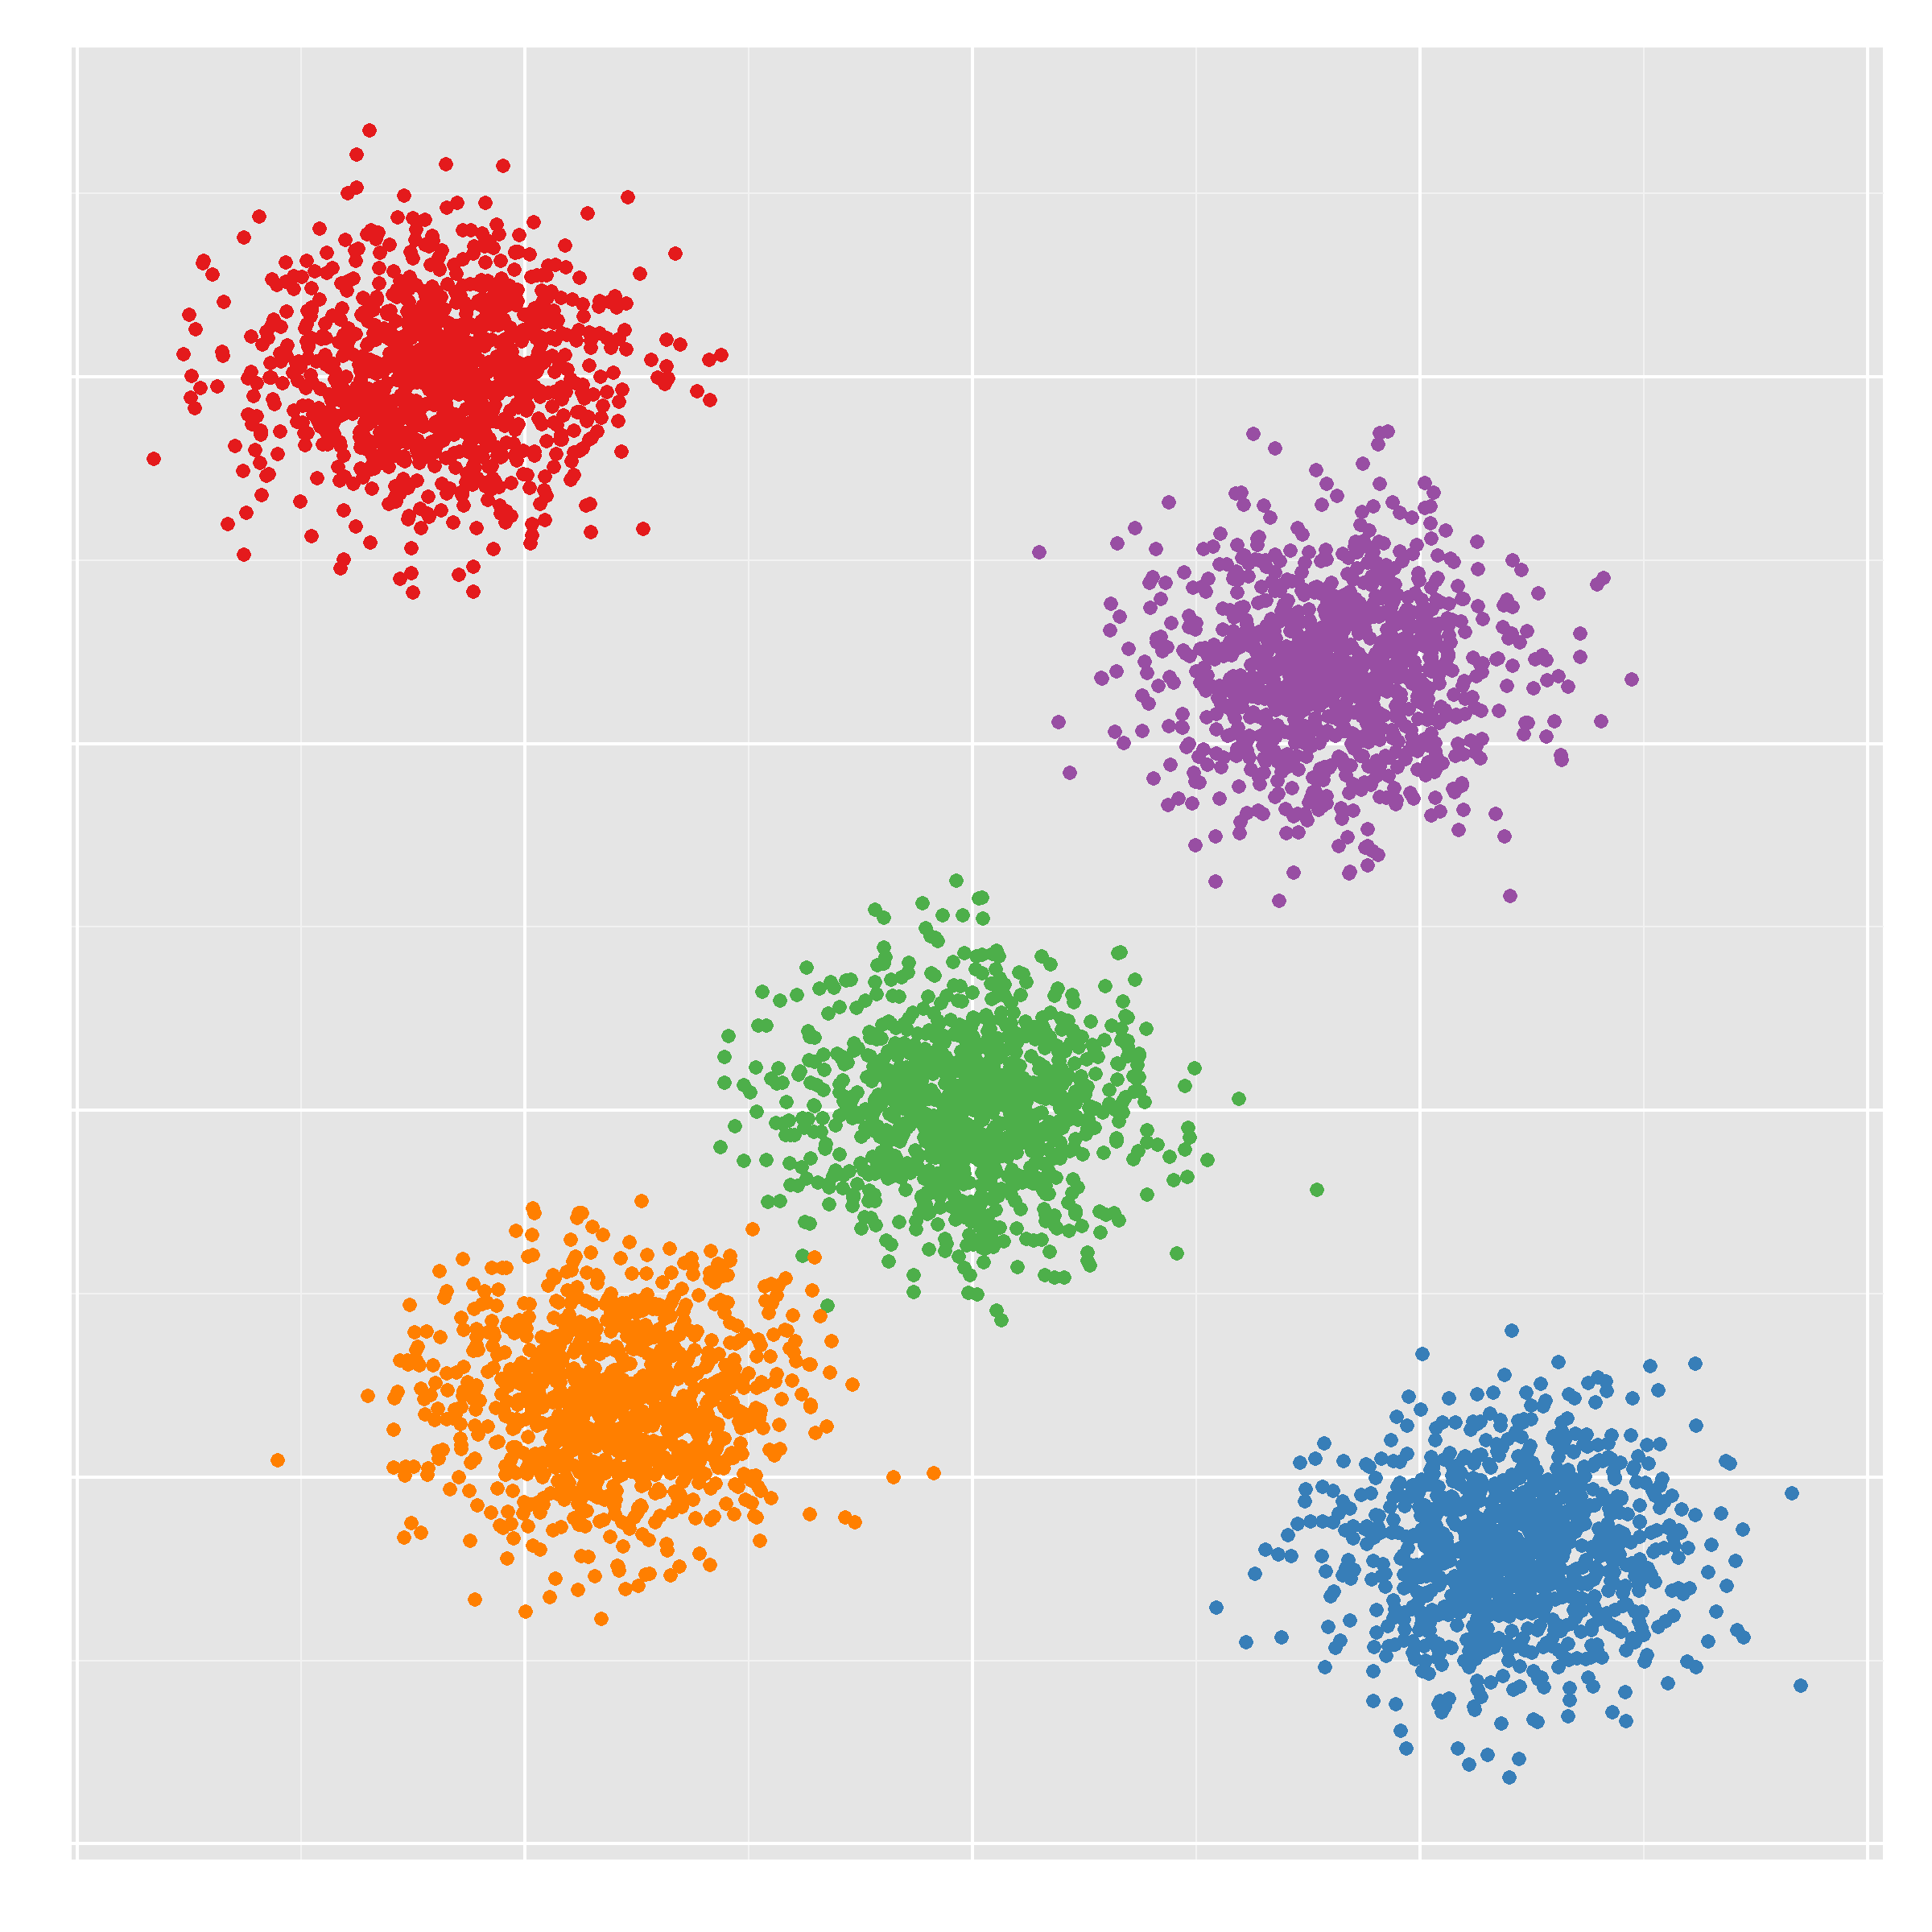
\includegraphics[width = 0.8\textwidth]{my_compact}
    \caption{Convex clusters.}
  \label{fig:compact}
  \end{subfigure}
  \begin{subfigure}{0.4\textwidth}
    \centering
    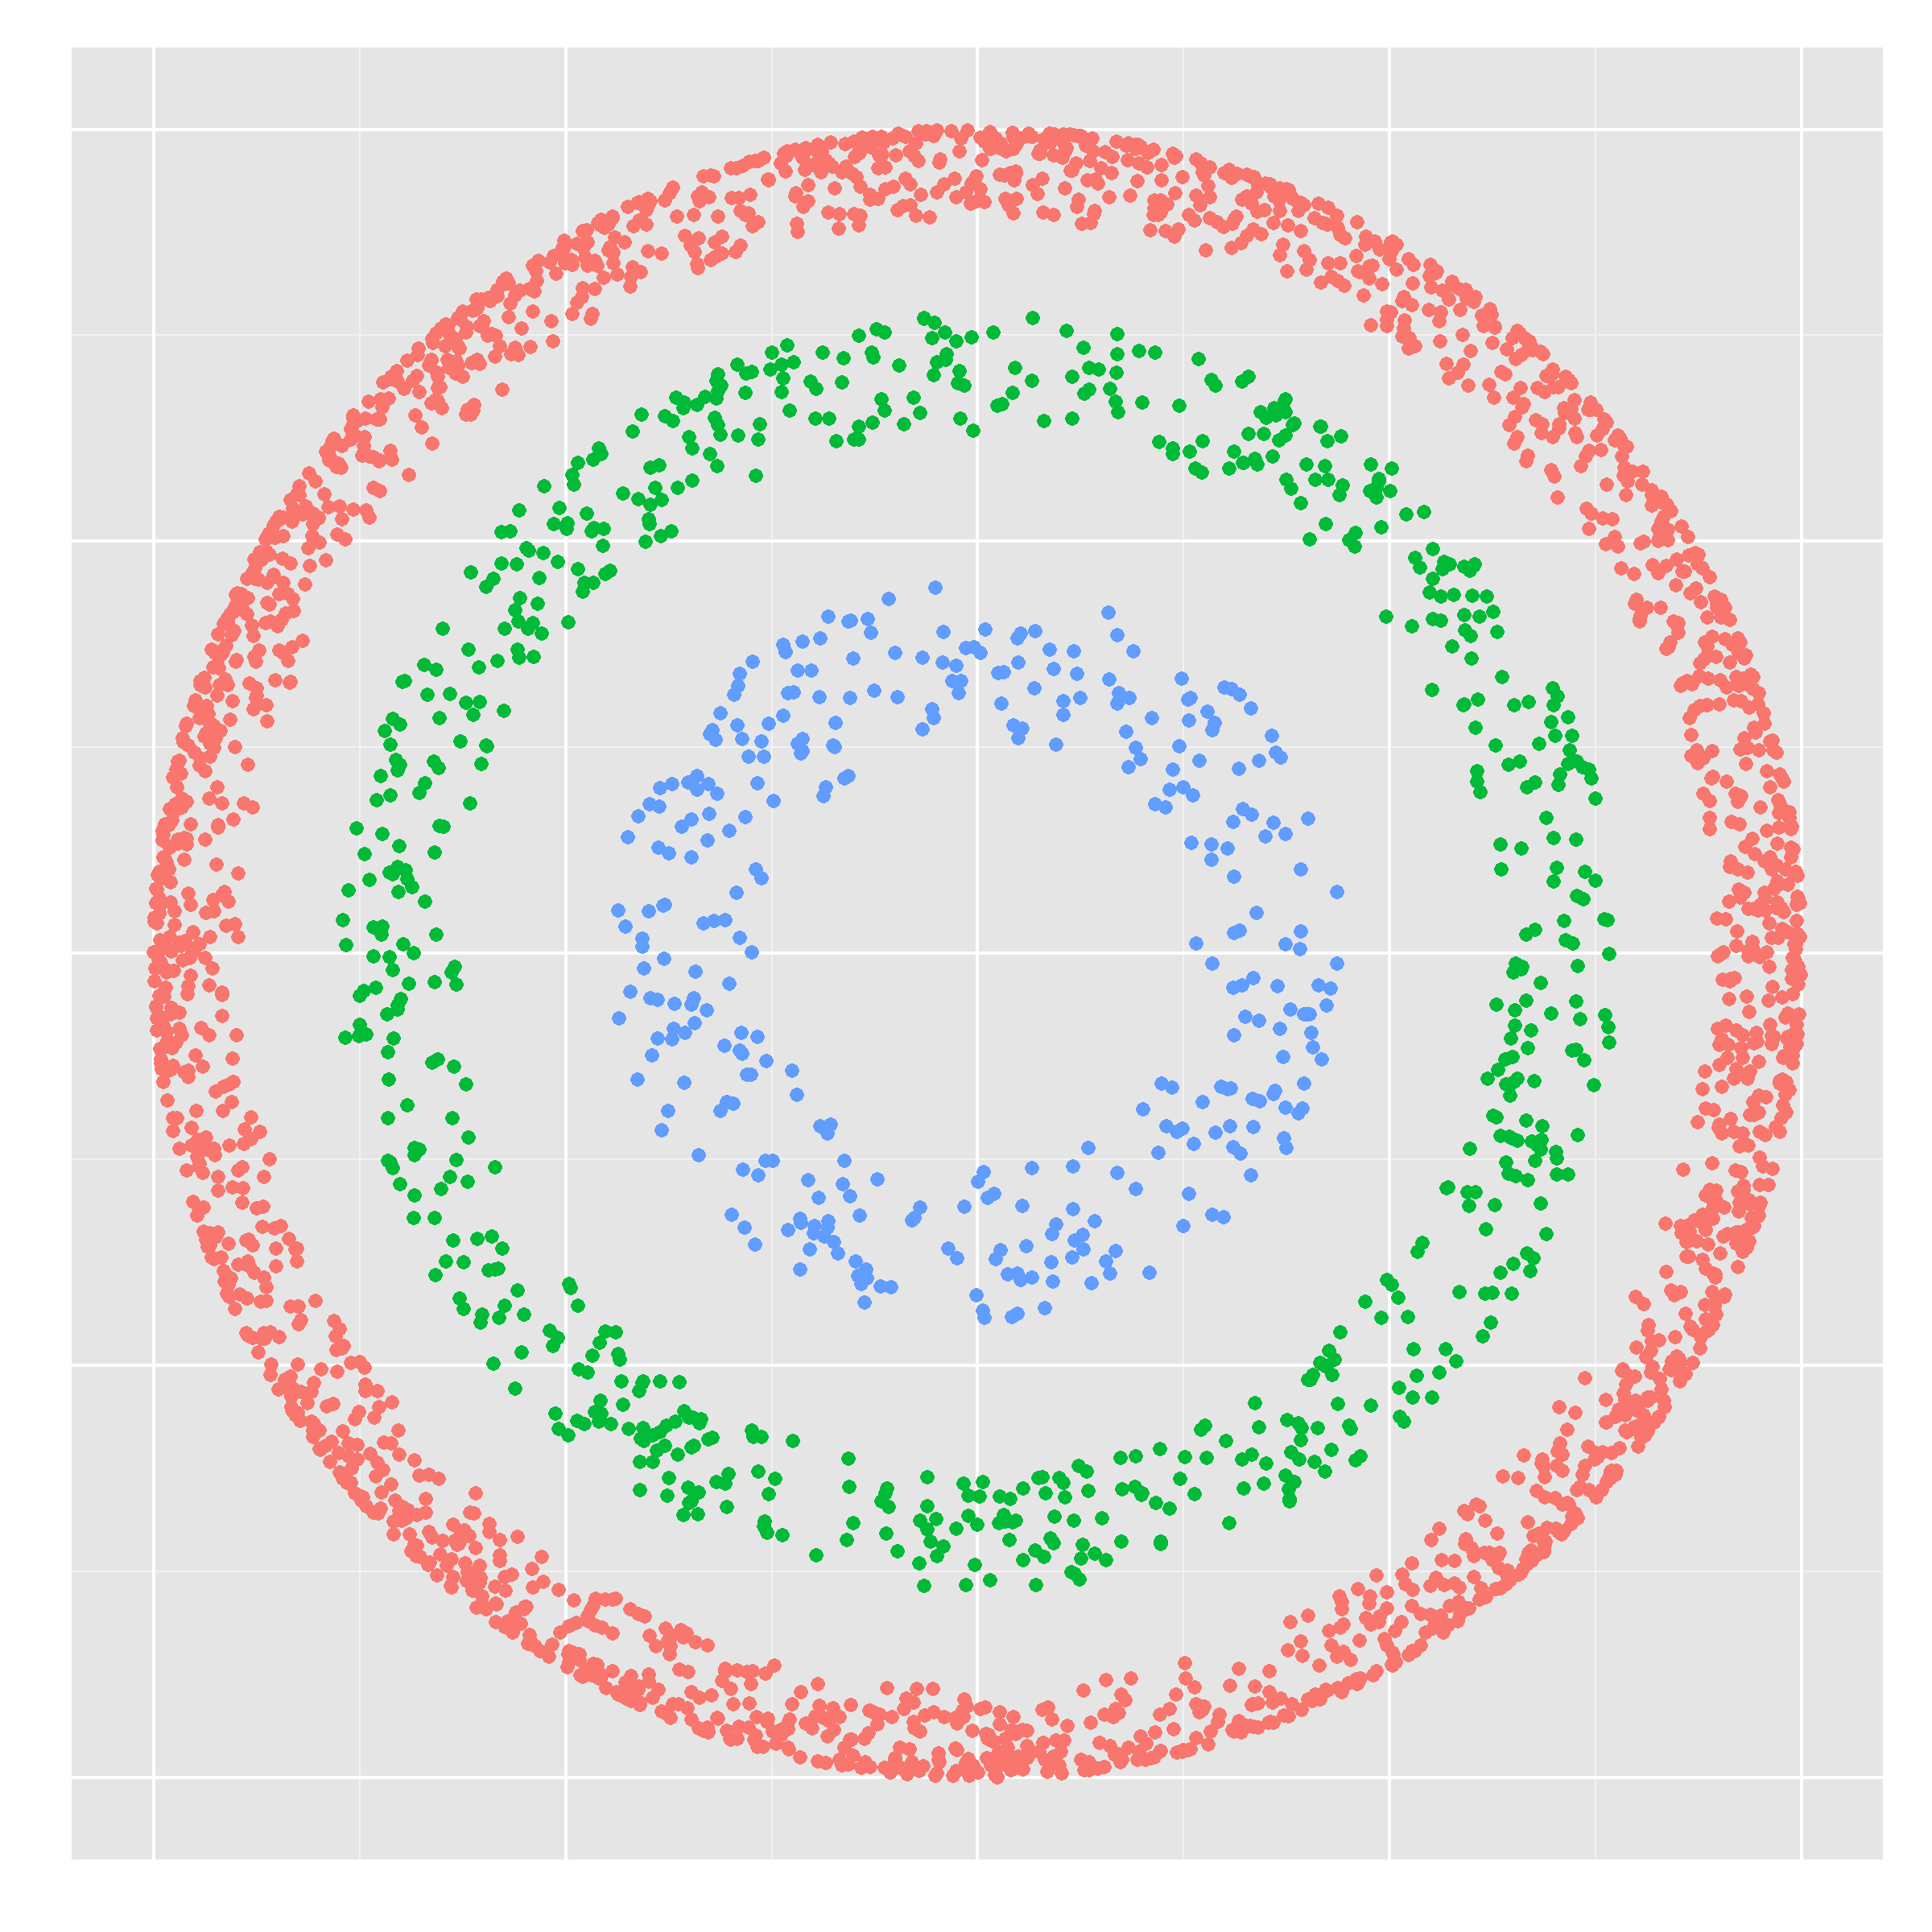
\includegraphics[width = 0.8\textwidth]{my_connected}
     \caption{Non-convex clusters.}
     \label{fig:connected}
     \end{subfigure}
  \caption{Examples of different types of clustering problems. The clusters in  Figure \ref{fig:compact} are generated by a multivariate Gaussian distribution.  The clusters in Figure \ref{fig:connected}  are non-convex which makes the clustering problem more difficult. }
  \label{fig:compact_connected}
\end{figure}

Simple clustering algorithms such as k-means are good at clustering data in which the underlying true clusters are convex \citep{Everitt2001}. An example of convex clusters is given in Figure \ref{fig:compact}. However k-means can fail when the true clusters are non-convex like those shown in Figure \ref{fig:connected}. This is because k-means is a centroid based clustering algorithm that clusters data based on how similar they are to cluster centroids. Spectral clustering instead clusters data based on how similar they are to all other data points, which can lead to good quality segmentation on even these difficult cases.  We do not formally address what is meant by similarity here, but will define this fully in Section \ref{sec:affinity}.

 %Data which is convex may be simple to cluster as the gaps between clusters are easy for simple clustering algorithms like k-means to identify. Connected but non-convex data sets can be much more challenging than convex data sets, and can cause some simple clustering algorithms to fail. The reason that centroid based clustering algorithms such as k-means struggle with data sets like that shown in Figure \ref{fig:connected} is that k-means clusters the data based on how similar they are to cluster centroids. spectral clustering instead clusters data based on how \textit{similar} they are to all other data points, which can lead to good quality segmentation on even these difficult cases.  We do not formally address what is meant by similarity here, but will define this fully in Section \ref{sec:affinity}.

The similarity between data points can be neatly represented in a graph structure.  We can then restate the clustering problem as a graph partitioning problem where we wish to find a partition of the graph such that the edges between different groups have low weights (which corresponds to data points being dissimilar) and the edges within a group have high weights (the data points are similar). In order to introduce spectral clustering we first introduce some graph notation and discuss graph cut problems. We will then describe the spectral clustering algorithm, and discuss in more detail the notion of similarity. 

\subsection{Graph cut problems} 

Data can be represented as a similarity graph, $G = (V,E)$ where each vertex $v_i \in V$ represents a data point $x_i$. The graph will be undirected, by which we mean the edges denote a two-way relationship.  The graph can then be described by an \textit{adjacency matrix}. Adjacency matrices are a way of depicting the graph structure with binary entries denoting which vertices are connected by edges and which are not. Figure \ref{fig:sim_graphs} depicts two similarity graphs and their corresponding adjacency matrices. A  value of $1$ in cell (2,3) implies that vertices $v_2$ and $v_3$ are connected by an edge. Note that both of the example adjacency matrices given below are symmetric, which can be expected as we are dealing with undirected graphs. 

\begin{figure}[H]
  \centering
   \begin{subfigure}{0.4\textwidth}
    \centering
    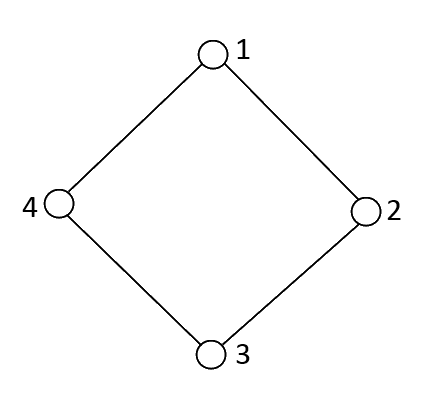
\includegraphics[width = 0.6\textwidth]{adj_square.png}
   \end{subfigure}
  \begin{subfigure}{0.4\textwidth}
    \centering
    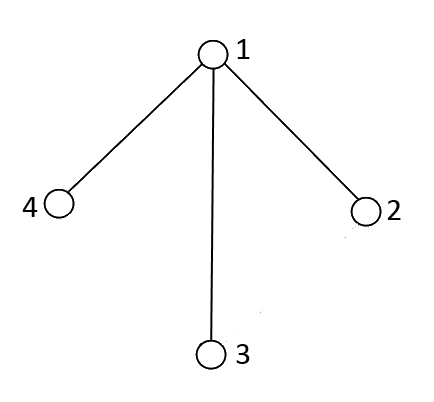
\includegraphics[width = 0.6\textwidth]{adj_tree.png}
  \end{subfigure}\\
\begin{equation*}
\renewcommand*{\arraystretch}{.5}
  \begin{pmatrix}
    0 & 1 & 0 & 1 \\
    1 & 0 & 1 & 0 \\
    0 & 1 & 0 & 1 \\
    1 & 0 & 1 & 0 
    \end{pmatrix}
\hspace{1.6in}
\renewcommand*{\arraystretch}{.5}
  \begin{pmatrix}
    0 & 1 & 1 & 1 \\
    1 & 0 & 0 & 0 \\
    1 & 0 & 0 & 0 \\
    1 & 0 & 0 & 0 
    \end{pmatrix}
\end{equation*}
\caption{Two example similarity graphs and their corresponding adjacency matrices.}
\label{fig:sim_graphs}
\end{figure}

The \textit{weighted adjacency matrix} (also called an \textit{affinity matrix}) of a similarity graph is the matrix $W = (w_{ij})_{i,j = 1,\ldots, n}$. The weight $w_{ij}$ is the similarity between vertices $v_i$ and $v_j$.  If $w_{ij}=0$, this means that the vertices $v_i$ and $v_j$ are not connected by an edge. Again the affinity matrix will be symmetric, that is $w_{ij} = w_{ji}$. 

In order to create a graph partition we need to cut the edges in the graph. Non-empty subsets of $V$, $A$ and $B$ will form a partition of the graph $G$ if $A \cap B = \emptyset  $ and $A \cup B = V$.  
The weight of the cut can be calculated by summing the weights of the edges which will be broken when a cut is made. In order to find a good partition of the graph, we wish to choose $A$ and $B$  such that some cut criterion is minimised.  The simplest cut criterion is

\begin{equation}
  \text{cut(A,B)} = \sum_{i \in A, j \in B} w_{ij},\\
  \label{eq:cut}
\end{equation}
where the notation $i \in A$ is short hand to mean the set of indices $\{ i | v_i \in A \}$.

The Minimum cut \citep{Wu1993} is the cut which minimises equation \eqref{eq:cut}. This can be solved in polynomial time \citep{Stoer1997} however the  minimum cut does not always produce a desirable graph partitioning; it tends to create unbalanced partitions, separating one vertex from the rest of the graph. To understand why this happens, note for a fully connected graph where all vertices are joined by an edge, the number of edges cut in mincut will be  $|A| \times |B|$ which is minimised by the solutions $|A| = 1$ or $|B| = 1$. In order to avoid this, we can specify that the sets $A$ and $B$ are reasonably large in some way. Two common objective functions used to avoid this issue are the RatioCut \citep{Hagen1992} and the normalised cut, Ncut \citep{Malik2000}. 

Both RatioCut and Ncut attempt to normalise the weight of the cut by introducing the size of sets $A$ and $B$. In RatioCut, the size of $A$ is measured by its number of vertices $|A|$, while in Ncut the size is measured by the weights of its edges $\text{vol}(A) = \sum_{i \in A}d_i$ where $d_i= \sum_{j = 1}^n w_{ij}$ is the \textit{degree} of a vertex $v_i \in V$. The definitions of RatioCut and Ncut are as follows, 

\begin{equation}
  \text{RatioCut(A,B)} = \frac{\text{cut} (A, B)}{|A|} + \frac{\text{cut}(A, B)}{|B|}, 
    \label{eq:ratiocut}
\end{equation}

\begin{equation}
  \text{Ncut(A,B)} = \frac{\text{cut}(A, B)}{\text{vol}(A)} + \frac{\text{cut}(A, B)}{\text{vol}(B)}.
    \label{eq:ncut}
\end{equation}

The main idea in Ncut is that large clusters will increase the denominator vol$(A)$ and thus decrease Ncut$(A,B)$. This will encourage splitting the data into fairly evenly sized clusters, and avoid the minimum cut issue of segmented isolated points. This can be seen in Figure \ref{fig:min_norm_cut}  which depicts both the minimum cut and Ncut solutions for a particular graph. The shaded/non-shaded regions represent the partitioning. The minimum cut isolates one vertex from the rest of the graph, whilst the Ncut provides a more balanced and sensible partition. 

\begin{figure}[H]
  \centering
  \begin{subfigure}{0.4\textwidth}
    \centering
    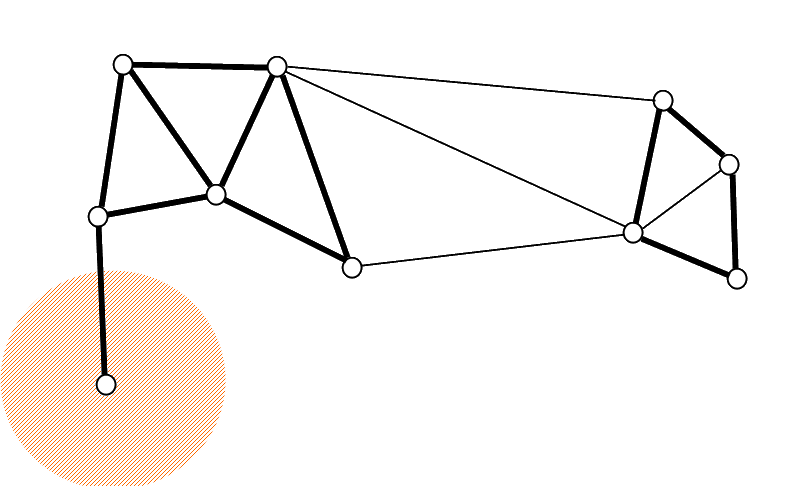
\includegraphics[width = \textwidth]{my_min_cut.png}
    \caption{Minimising the cut.}
  \label{fig:min_cut}
  \end{subfigure}
  \begin{subfigure}{0.4\textwidth}
    \centering
    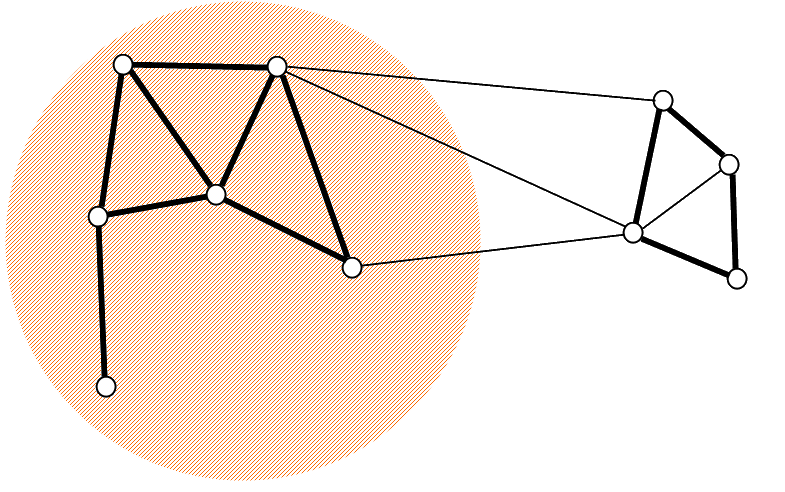
\includegraphics[width = \textwidth]{my_norm_cut.png}
  \caption{Minimising the normalised cut.}
  \label{fig:norm_cut}
  \end{subfigure}
  \caption{Two solutions to the bi-partition problem. The partitioning is indicated by shading/non-shading of nodes.}
  \label{fig:min_norm_cut}
\end{figure}

Although the partitioning has been improved, the previously easy to solve mincut problem (equation \ref{eq:cut}) has been replaced with minimising the normalised cut (equation \ref{eq:ncut}) which is an NP-hard problem \citep{Wagner1993}. Therefore,  a continuous relaxation of the Ncut is solved instead. The solution to the relaxed problem of equation \eqref{eq:ncut} is given by the second eigenvector of the symmetric graph Laplacian defined in equation \eqref{eq:laplacian_symm} \citep{Luxburg2008}. Similarly, the solution of the relaxed problem the ratio cut (equation \ref{eq:ratiocut}) is given by the second eigenvector of the unnormalized Laplacian defined in equation \eqref{eq:laplacian}. Here $W$ is the affinity matrix of the similarity graph and the degree matrix $D$ is defined as the diagonal matrix with the degrees $d_1, \ldots d_n$ on the diagonal. The relaxation of these graph cut problems into the eigen-decompostion of Laplacian matrices is the basis of spectral clustering. 
 %It has been shown that the two graph cut optimisations given in equations \eqref{eq:ratiocut} and \eqref{eq:ncut} can be formulated in terms of the spectral decomposition of the graph Laplacian matrices given in equations \eqref{eq:laplacian} and \eqref{eq:laplacian_symm} respectively.  

\begin{eqnarray}
\label{eq:laplacian}
 L =& D - W.\\
\label{eq:laplacian_symm}
 L_{\text{symm}} =& D^{-1/2}LD^{-1/2}. 
\end{eqnarray}


Unfortunately, there is no guarantee on the quality of the solutions of the relaxed problems compared to the exact solutions \citep{chung1997spectral}. Consequently, it has been shown that some pathological cases exist which are arbitrarily bad. However, several papers which investigate the quality of the clustering of spectral clustering \citep{Spielman1996, Kannan2004} find spectral clustering to provide good solutions. 

The spectral clustering algorithm that we use \citep{Ng2001} uses the symmetric Laplacian  $L_{\text{symm}}$ as defined in equation \ref{eq:laplacian_symm}. The full spectral clustering algorithm is given in Algorithm \ref{alg:njw}. Note that the number of clusters is assumed to be known and this will be the case throughout this chapter.


\begin{algorithm}
\caption{NJW spectral clustering algorithm}
\begin{algorithmic}[1]
\REQUIRE Data set $X = \{x_1,\ldots, x_n \}$, number of clusters $k$.
\ENSURE $k$-way partition of the input data.
\STATE Construct the affinity matrix $W = (w_{ij})_{i,j = 1,\ldots, n}.$ %by the following Gaussian kernel function:
%\begin{equation*}
 % w_{i,j} = \exp  \left( - \frac{\| x_i - x_j \|^2}{2 \sigma^2} \right), i,j = 1, \ldots,n.
%\end{equation*}

\STATE Compute the symmetric Laplacian matrix  $L_{\text{symm}} = D^{-1/2}( D - W )D^{-1/2}$, where $D$ is the diagonal matrix with $D_{ii}=\sum_{j=1}^{n} w_{ij}.$
\STATE Compute the $k$ eigenvectors of $L_{\text{symm}}$, $v_1, v_2,\ldots , v_k,$ associated with the $k$ smallest eigenvalues, and form the matrix $ V = [v_1,v_2, \ldots ,v_k]$.
\STATE Renormalise each row of $V$ to form a new matrix $Y$.
\STATE Partition the $n$ rows of $Y$ into $k$ clusters using  k-means.
\STATE Assign the original data point $x_i$ to the cluster $l$ if and only if the corresponding row $i$ of the matrix $Y$ is assigned to the cluster $l$.
\end{algorithmic}
\label{alg:njw}
\end{algorithm}

Once the Laplacian has been calculated, one computes the $k$ eigenvectors which correspond to the $k$ smallest eigenvalues of the Laplacian. A matrix $Y \in \mathbb{R}^{n \times k}$ is created, where each column is an eigenvector of the Laplacian, with length $n$. We can view this matrix $Y$ as an embedding of the original data $X$ into a lower dimensional subspace. When represented in this low subspace the clustering problem is often easier, and can be solved with a simple clustering algorithm such as k-means. For example, Figure \ref{fig:spirals_original} shows a data set of three spirals depicted in the original feature space. This is visually quite difficult to cluster. Figure \ref{fig:spirals_embedded} plots the same data set but embedded in the lower dimension, plotting the first eigenvector of the Laplacian against the second eigenvector. Clustering in the embedded space is easy even for k-means to solve. 


\begin{figure}[h!]
  \centering
  \begin{subfigure}{0.4\textwidth}
    \centering
    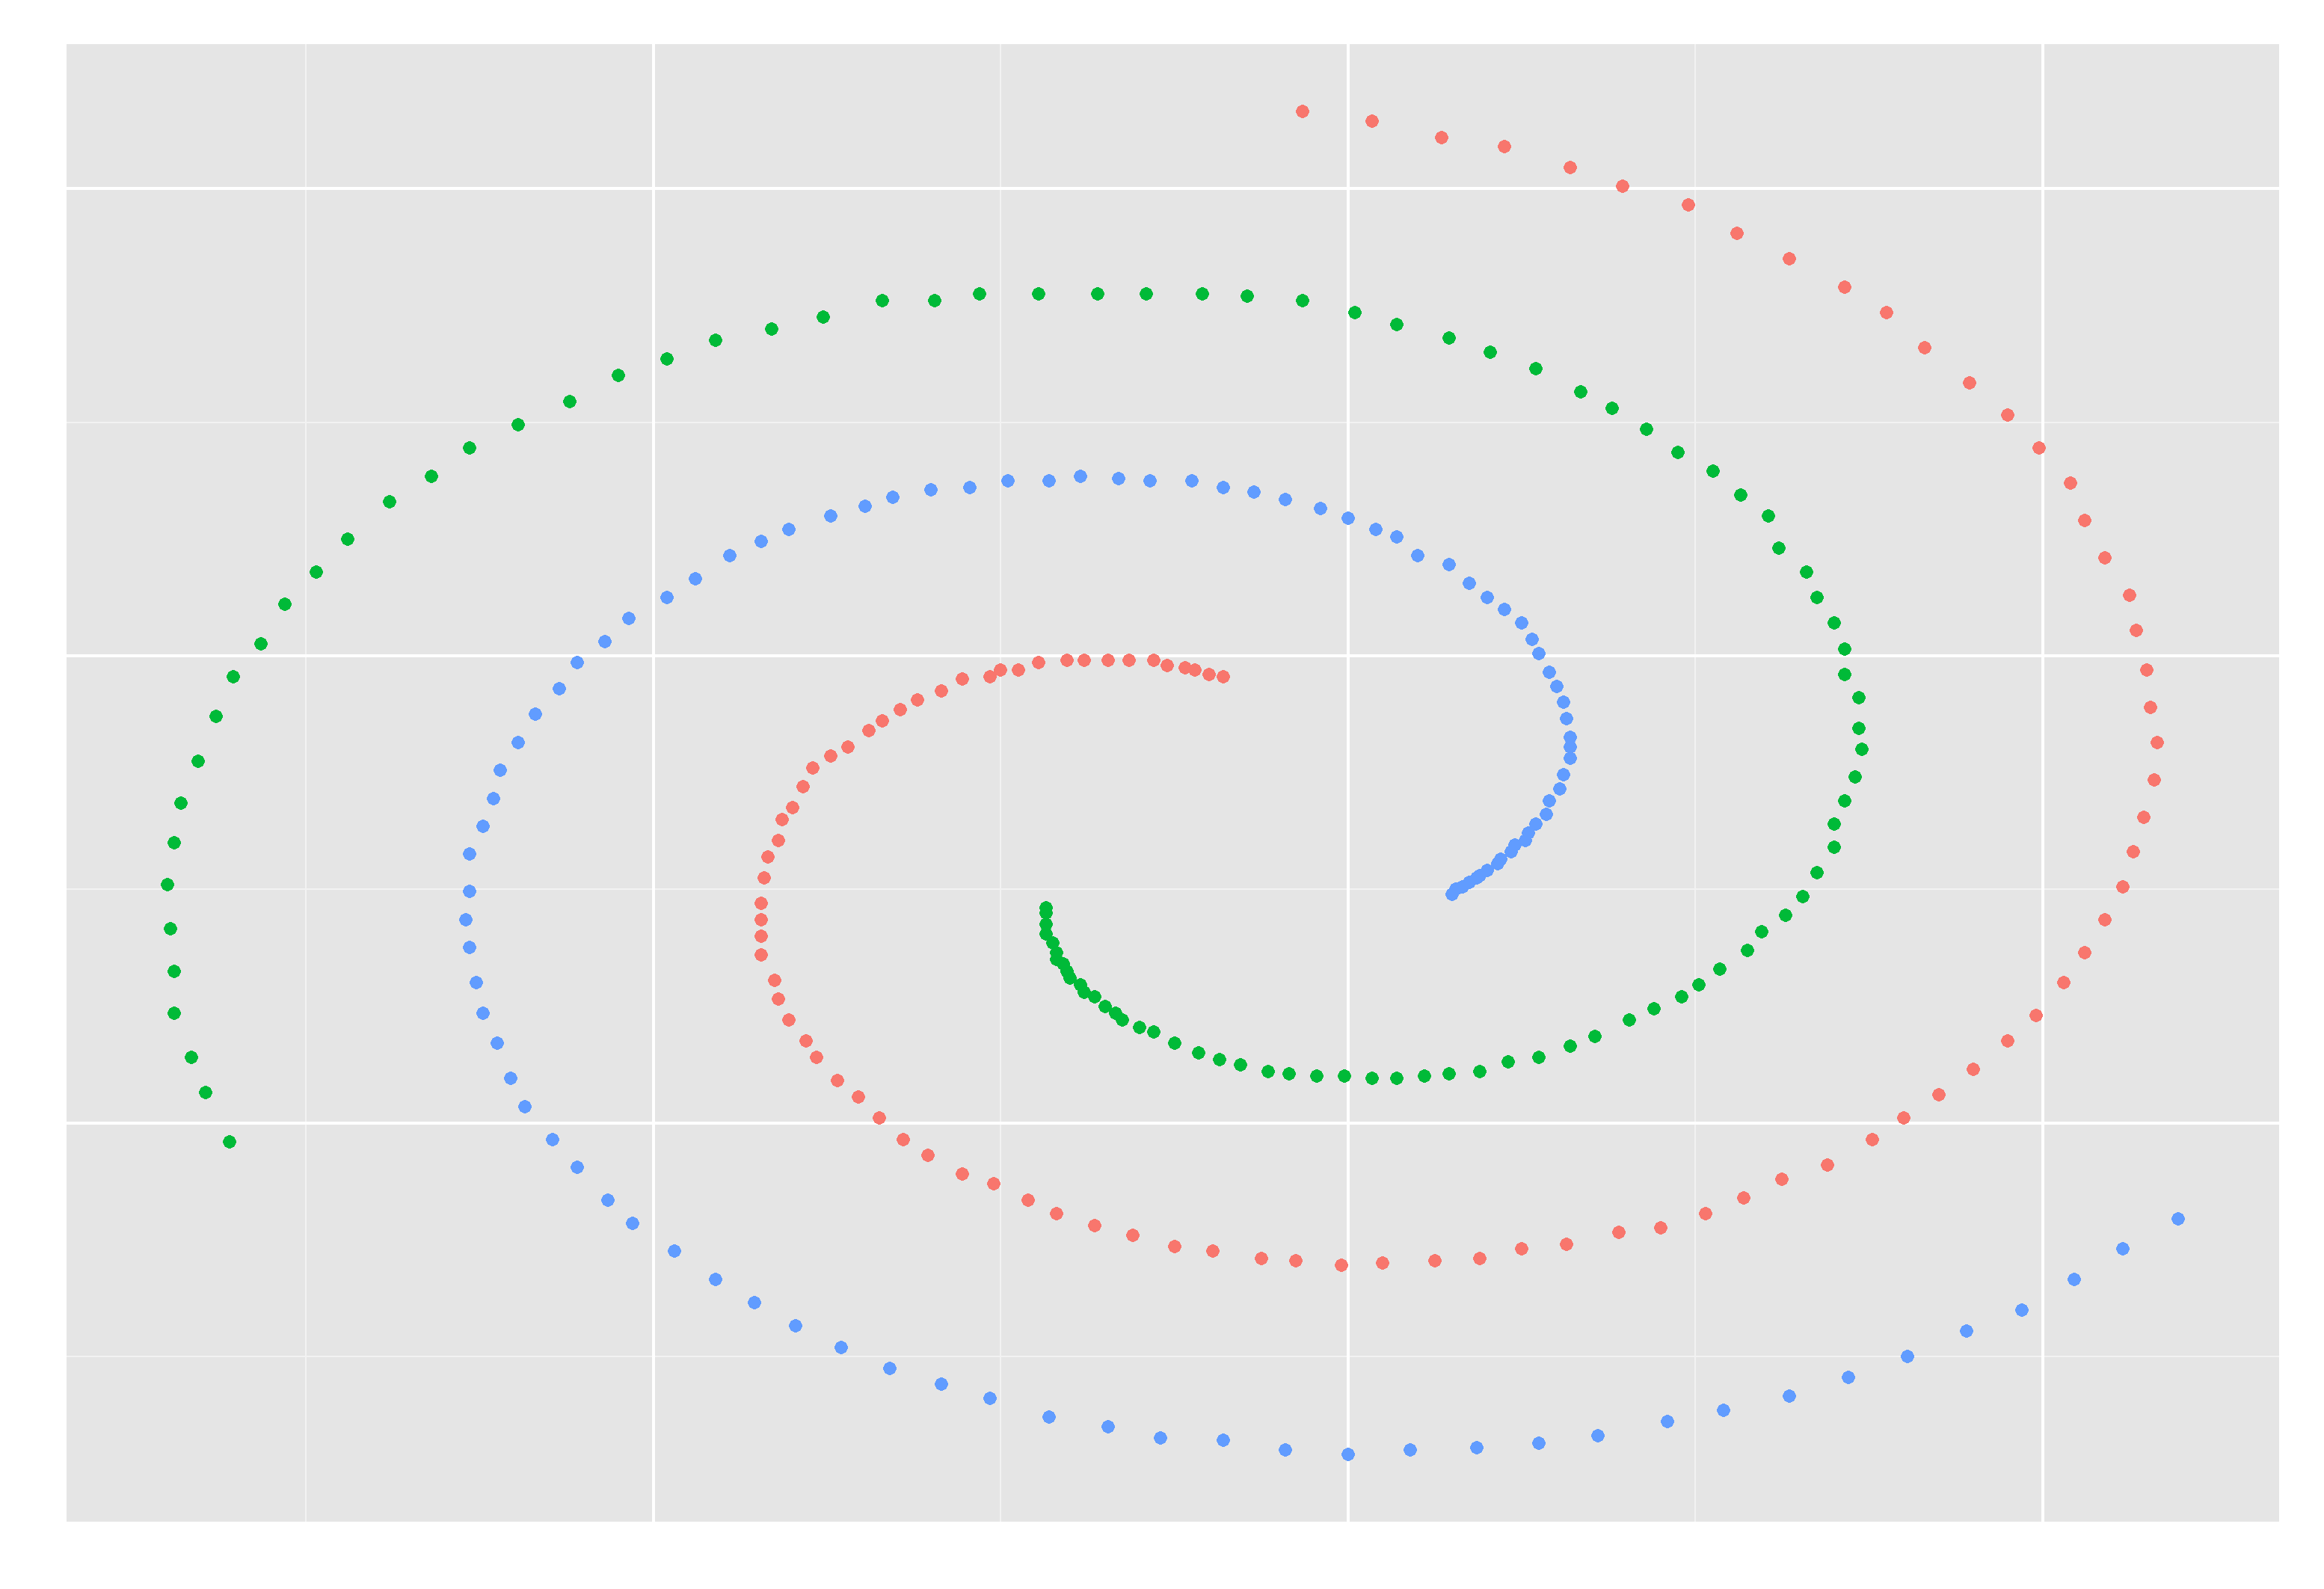
\includegraphics[width = \textwidth, height = \textwidth]{code_embedding/3_spiral_original.png}
    \caption{Data viewed in the original \\ feature space.}
  \label{fig:spirals_original}
  \end{subfigure}
  \begin{subfigure}{0.4\textwidth}
    \centering
    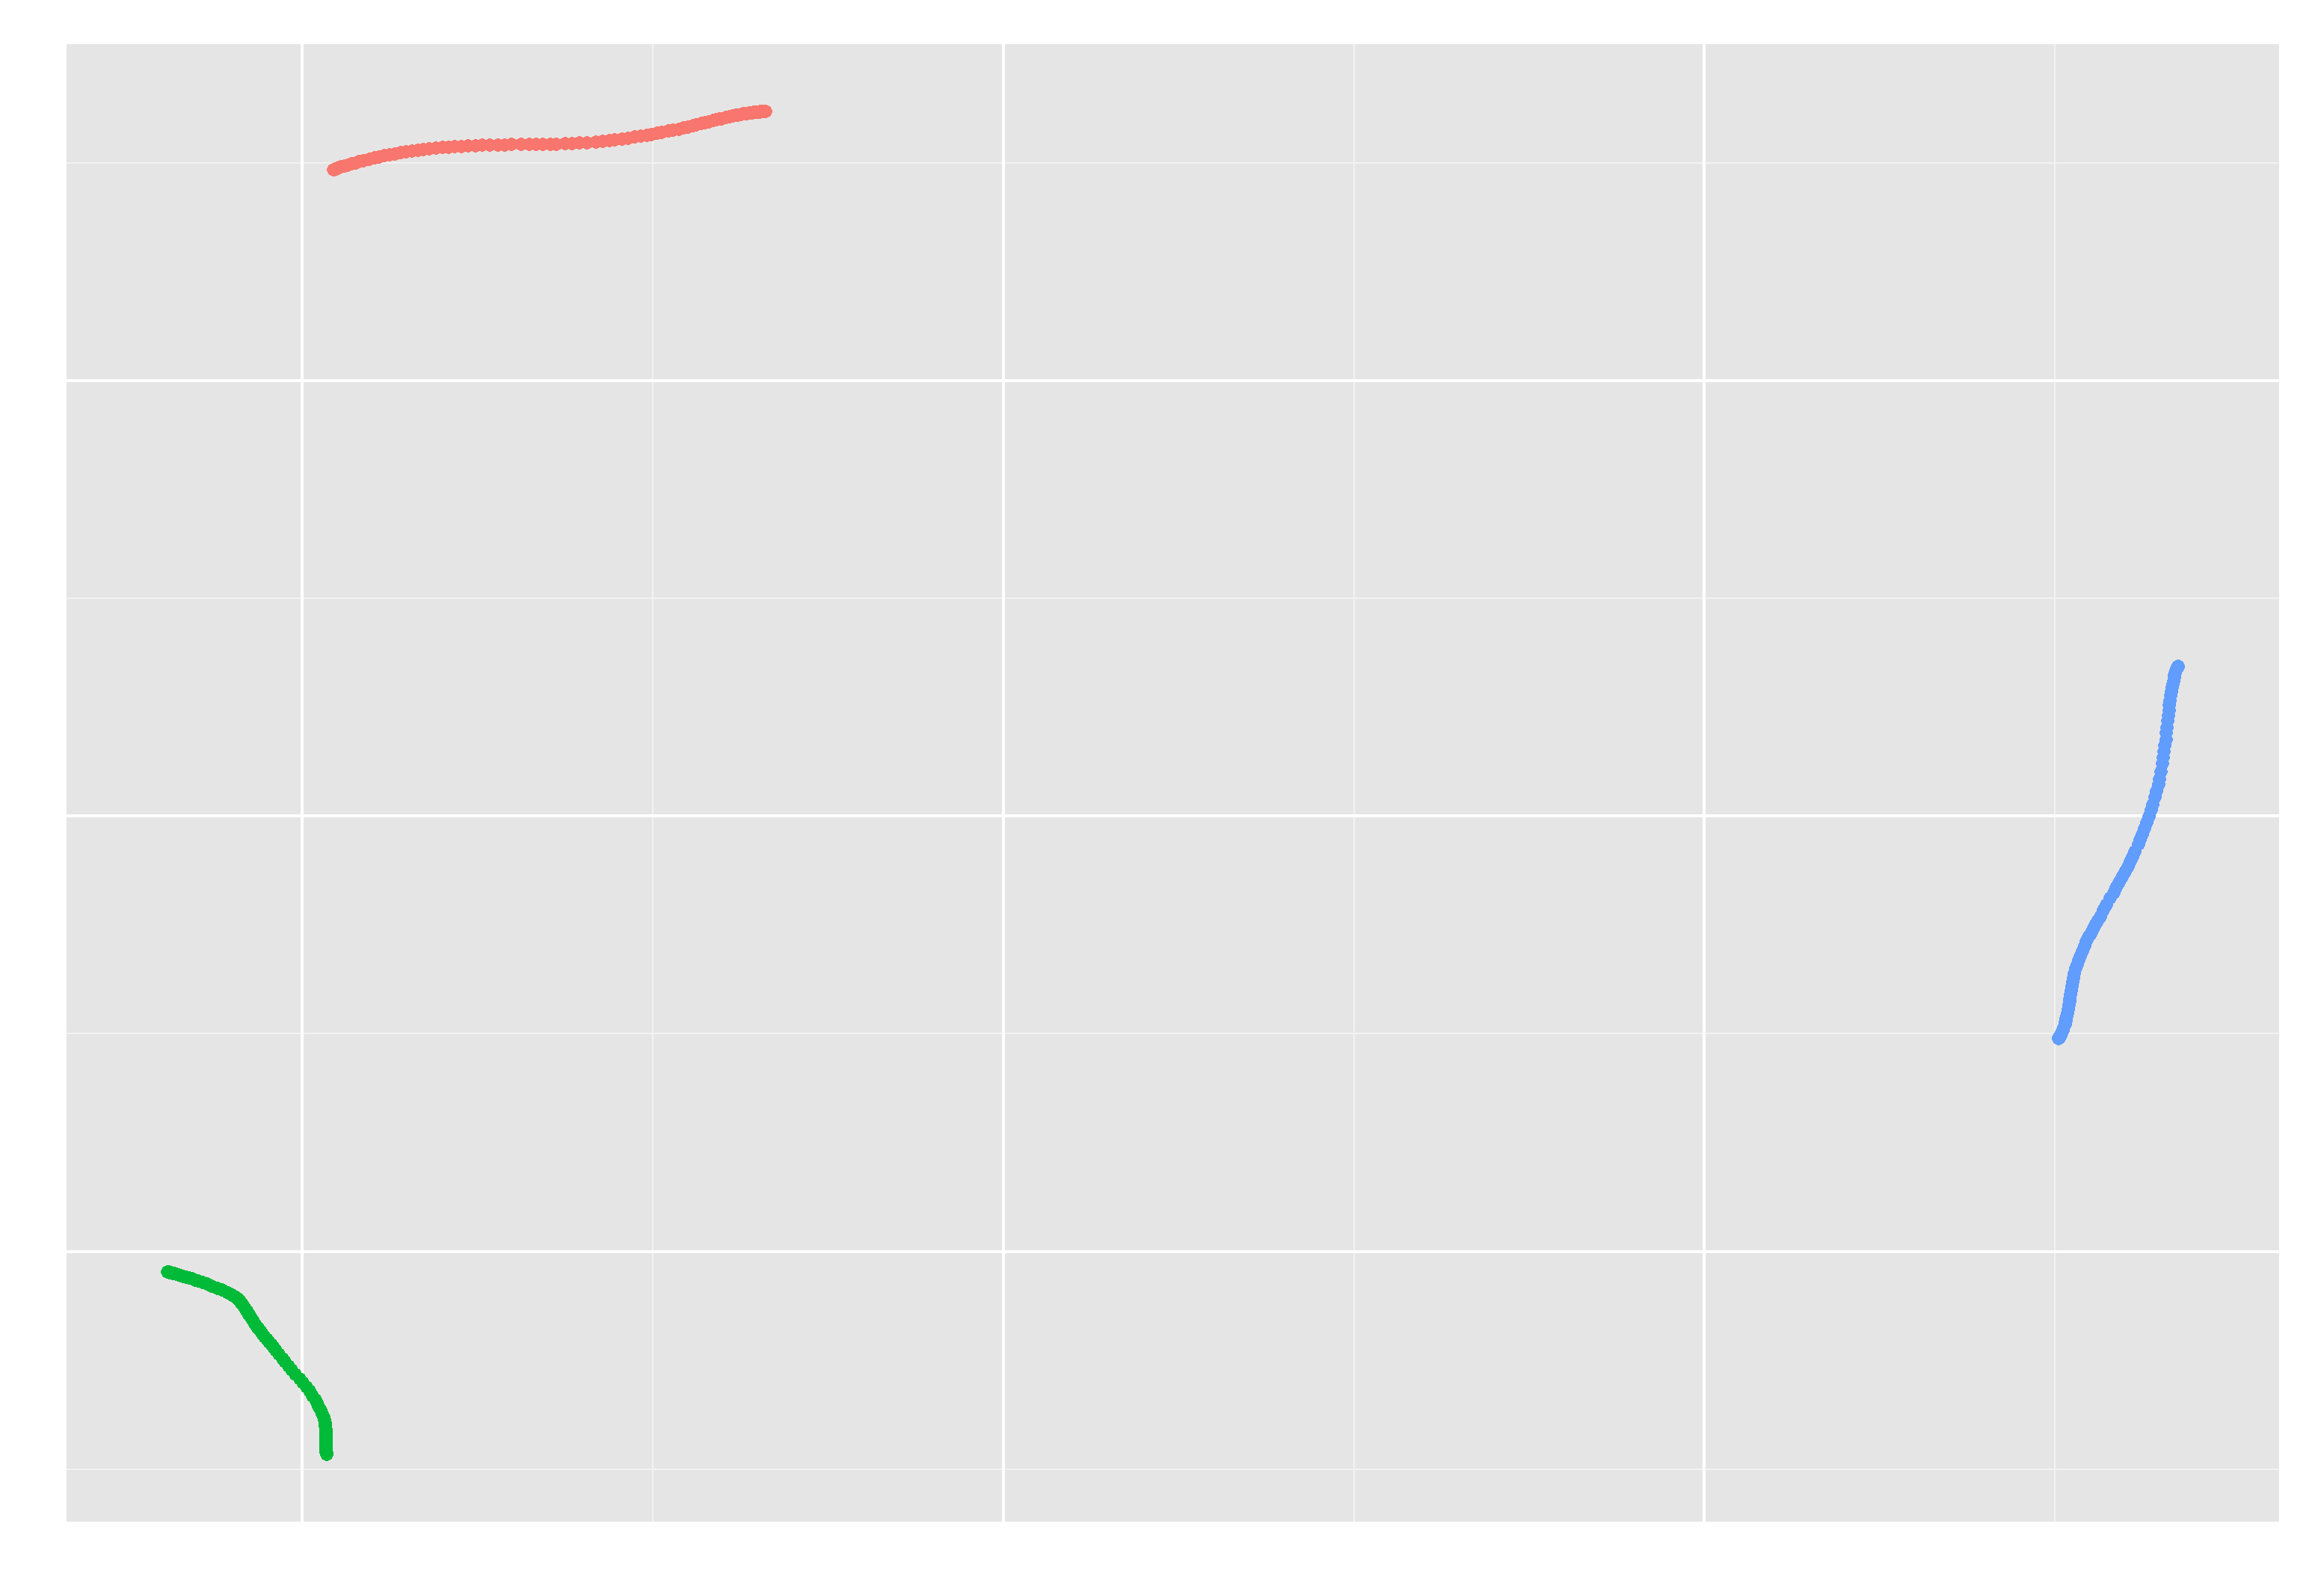
\includegraphics[width =\textwidth, height = \textwidth]{code_embedding/3_spiral_embedded.png}
     \caption{Data viewed in the 2-dimensional \\ embedding space. }
     \label{fig:spirals_embedded}
     \end{subfigure}
  \caption{Triple spiral data set viewed in feature space (a) and eigenvector space (b).}
  \label{fig:triple_spirals}
\end{figure}


After the embedding, k-means can be used to cluster the $n$ rows of $Y$ into $k$ clusters. Finally, assign the cluster label given to each row $Y_i$ to the corresponding original data point $x_i$. Now that we have introduced the general spectral clustering algorithm, we will discuss the notion of similarity in more detail.

\subsection{Choice of affinity matrix}
\label{sec:affinity}

One of the key factors of spectral clustering is the affinity matrix $W = (w_{ij})_{ i,j = 1, \ldots, n}$  which represents the pairwise similarities between all data points $x_i$ and $x_j$. A popular choice is to use the Gaussian kernel, 

\begin{equation}
  \label{eq:gaussian_affinity}
    w_{i,j} = \exp  \left( - \frac{\| x_i - x_j \|^2}{2 \sigma^2} \right), \; i, j = 1, \ldots, n,
\end{equation}
where the parameter $\sigma$ controls the width of the local neighbourhoods which we want to model. If $x_i$ and $x_j$ are very close, then $w_{ij} \rightarrow 1 $, and if they are far apart $w_{ij} \rightarrow 0$. A Gaussian kernel affinity matrix will have ones along the diagonal and is symmetric $(w_{ij} = w_{ji})$.

The scaling parameter $\sigma$ is usually chosen manually. \cite{Ng2001} automatically choose $\sigma$ by running their clustering algorithm repeatedly for a number of values of $\sigma$. They then select the $\sigma$ which provides least distorted k-means clusters in step 5 of Algorithm \ref{alg:njw}. \cite{Zelnik-Manor2004} argue that for data which has a cluttered background, or multi-scale data, one global parameter choice for $\sigma$ is not sufficient. They calculate a localised parameter $\sigma_i$ for each data point $x_i$ based on its neighbourhood. Using a localised $\sigma_i$ can deal well with multi-scale data, but requires the user to choose the size of the neighbourhood in order to calculate $\sigma_i$. 

If we mainly wish to model the local relationships then using all of the possible pairwise data similarities may not be necessary. It is possible to use a weighted k-nearest neighbour structure \citep{Luxburg2008} to build the affinity matrix once corrections have been made to ensure that this matrix is symmetric. Another option is to choose some threshold $\epsilon$ and only consider connections between data points whose pairwise similarities are greater  than this threshold $\epsilon$. This is an $\epsilon$-neighbourhood graph as shown in equation \eqref{eq:epsilon_graph}. 

%Although it is possible to weight this graph by $\epsilon$, if we choose $\epsilon$ to generate a small $\epsilon$-neighbourhood, then the differences between the weights will be so small that weighting may become eligible.

\begin{equation}
\label{eq:epsilon_graph}
  w^*_{ij}=\left\{
  \begin{array}{@{}ll@{}}
    1, & \text{if}\ w_{ij} > \epsilon \\
    0, & \text{otherwise.}
  \end{array}\right.
\end{equation} 

Using this construction will give a sparse affinity matrix instead of a fully connected graph, which will help lower the computational complexity. 

\section{Advanced Spectral Clustering}
\label{sec:ad_spec}

In the previous section we introduced spectral clustering via graph partitioning and discussed options for creating affinity matrices. Our overall aim is to perform spectral clustering on data streams. First, we consider some of the challenges that make clustering in data streams so difficult, and look at the approaches that exist to deal with these challenges in the spectral clustering setting.

 The first challenge that is addressed is dealing with big data. One of the main difficulties in data streaming is the pure volume of data available and the methods discussed in Section \ref{sec:big_data} offer methods to perform spectral clustering on big data.  Another difficulty that arises in data streaming is the ability to update the current clustering result  as new data arrives.  Incremental spectral clustering is a potential solution to this challenge and is discussed in Section \ref{sec:incremental}.

It is stressed that these problems (large data and incremental data) are just sub-problems of what makes data streaming difficult. In particular, none of the methods described below are capable of dealing with data streams which are unbounded in length.  The solutions offered in the next section to speed up computation for large data sets cannot update the clustering result if a new data point arrives. The incremental spectral clustering algorithms can update cluster membership as new data arrives but do not scale as for very large or possibly infinite $n$. %The even more challenging setting of data streams, will be addressed in Section \ref{sec:microSpec}.    

\subsection{Large-scale Spectral Clustering}
\label{sec:big_data}

%Although spectral clustering has been shown to perform well empirically on simple data sets, computational problems arise as the data set size increases.  
Spectral clustering can be challenging for very large data sets since constructing the affinity matrix $W$ and computing the eigenvectors of $L$ have computational complexity $\mathcal{O}(n^2)$ and $\mathcal{O}(n^3)$ respectively. The Nystr\"{o}m method \citep{Williams2001} is a general method for generating good quality low rank approximations of large matrices. The Nystr\"{o}m approximation method for spectral clustering \citep{Fowlkes2004} randomly samples the columns of the affinity matrix $W$ and approximates the eigen decomposition of the full matrix directly using correlations between the sampled columns and the remaining columns. Effectively this can be thought of as a dial which the user has control over, sampling more columns will provide better results but at a higher computational cost. The downsides with this method are that the  memory requirements can be high and the random sampling of columns may lead to small clusters being under represented or completely missed in the final clustering. 
%Doesn't use the affinity to choose which columns in the matrix to sample.
%Fixed complexity dependant on the number of verticies $n$ and the number of samples columns $q$
%DRINEAS/MAHONEY non-uniform sampling of the Gram matrix and bounds approximation error
%But may need to sample many columns (O(n)?)
%practicaltiy on massive datasets may be limited according to Yan. (how big is massive?)
%DRINEAS/MAHONEY non-uniform sampling of the Gram matrix and bounds approximation error
%But may need to sample many columns (O(n)?)

% spectral clustering is performed on the representative set only, which is significantly faster than performing spectral clustering on the full data set. The resulting cluster labels for the representative data are linked back to the original data set such that every original data point acquires the same label as its associated $k$-means cluster centre. 

An alternative to the Nystr\"{o}m method is to use a pre-processing technique to reduce the size of the data. A natural way to do this is to select certain representative points to summarise the whole data set.  \cite{Yan2009} proposed KASP and RASP, algorithms which use k-means and random forest methods respectively to select $q$ representative points to apply spectral clustering on.  Similarly \cite{Shinnou2008} also use $k$-means to identify representative points, but in addition to using these points, \cite{Shinnou2008} also include any data points which are deemed to be suitably far from any representative point in the spectral clustering.  In both \cite{Yan2009} and \cite{Shinnou2008} the cluster labels given to the original data points are the same as the label assigned to their nearest representative point. As an alternative, \cite{Chen2011} represents the data as a linear combination of representative points. Random sampling has been applied to reduce the size of the data points within the eigen-decomposition step. \cite{Chen2006a, Liu2007} introduce early stopping strategies to speed up eigen-decomposition based on the observation that well-separated data points will converge more quickly to the final embedding. However this is only suitable for binary clustering.  Other possibilities include random projection with sampling methods \citep{Sakai2009} and shortest path methods \citep{Liu2013b}.

%\cite{Chen2011} has a ``landmark `` based SC.  $q$ landmark points are chosen to represent the data (randomly or with k-means), and the rest of the data is represented as a linear combination in a codebook type formar. % $\mathcal{O}(nq)$ and $\mathcal{O}(q^3 + q^2n)$. 

We discuss the KASP algorithm in more detail as it is the most popular speed up method for spectral clustering and it inspired our work in online spectral clustering which is introduced in Section \ref{sec:microSpec}.

In KASP, k-means is applied with $q$ clusters to the data set $X$, where $q$ is chosen such that $k \ll q \ll n$. Therefore each point in $X$ belongs to a cluster $y_j, (j \in 1, \hdots, q)$. Let the centres of these $q$ clusters be  $\widehat{y_1}, \hdots, \widehat{y_q}$. These  are used as representative points for the whole data set. Spectral clustering is performed on the representative points, reducing the complexity of the eigen decomposition from $\mathcal{O}(n^3)$ to $\mathcal{O}(q^3)$. Finally, the original data points are assigned the cluster label  that their closest representative point $\widehat{y_j}$ was assigned in the spectral clustering. The KASP algorithm is given in Algorithm \ref{alg:kasp}.

\begin{algorithm}[h!]
\caption{KASP}
  \begin{algorithmic}[1]
   \REQUIRE Data set $X = {x_1,\ldots, x_n}$, number of clusters $k$, number of representative points $q$.
   \ENSURE  $k$-way partition of the input data.
   \STATE Perform k-means with $q$ clusters on $x_1, \hdots, x_n$ to create clusters $y_1, \hdots y_q$.
   \STATE Compute the cluster centroids $\widehat{y_1}, \hdots, \widehat{y_q}$ as the $q$ representative points.
   \STATE Build a correspondence table to associate each $x_i$ with the nearest cluster centroids $\widehat{y_j}$.
   \STATE Run a spectral clustering algorithm on $\widehat{y_1}, \hdots, \widehat{y_q}$ to obtain an $k$-way cluster membership
   for each of $\widehat{y_j}, (j \in 1 \hdots q)$.
   \STATE Recover the cluster membership for each $x_i$ by looking up the cluster membership of the corresponding centroid $\widehat{y_j}$ in the correspondence table.
  \end{algorithmic}
\label{alg:kasp}
\end{algorithm}

Both KASP and RASP have been shown to perform well empirically on large data sets \citep{Yan2009}, retaining good clustering performance even as the \textit{data reduction ratio} increases. We can express the data reduction ratio as $\gamma = \frac{n}{q}$. As in many of the sampling methods discussed above, in KASP the user has control over the data reduction rate. A larger value of $q$ will give a better performance but at a computational cost. The KASP authors present an upper bound on the misclustering rate given the perturbation to the original data. This bound tells us how different the clustering output is if we use the full data set to cluster compared with if we just use the representative points. However, there are a number of assumptions required \citep{Huang2008} relating to the ability for the data to be separated into clusters. Also, this bound does not inform us about the quality of the clustering generally, only as a comparison to clustering the full data set. Finally, the method of assigning data points to clusters based on the cluster label of their representative point can lead to poor segmentation as shown in \cite{Cao2014}. They propose a local interpolation in their algorithm Local Information-based Fast Approximate spectral clustering (Li-ASP) to prevent this poor segmentation issue. They achieve this by assigning data points based on a weighted version of their $p$ closest representative points labels, rather than labelling based just on the label of the single closest representative point. 
 
% One constant challenge in clustering is selecting the number of clusters to search for. \cite{Zelnik-Manor2004} present a method for automatically choosing the true number of clusters using the eigenvectors to inform their choice. More commonly the eigenvalues are used to estimate the number of clusters, but if the clusters are not clearly separated identifying the number of clusters from eigenvalues alone is not trivial. We shall assume that the true number of clusters is known. 

The methods discussed above only address dealing with large data sets which are static. Our aim is to investigate methods which can update the spectral clustering partitioning when new data points arrive. 

\subsection{Incremental methods for Spectral Clustering}
 \label{sec:incremental}

Incremental spectral clustering methods are spectral clustering algorithms which are able to update their cluster partitioning when a new data point or batch of data point arrives. The term incremental is used here rather than online because although these algorithms can update when new data points arrive, they are not designed to deal with the full data streaming scenario. As a reminder, data streams are defined by the constant arrival of data points at a high velocity relative to the available processing power. On the other hand, incremental spectral clustering algorithms are designed for the problem of an evolving data set. For example, lets say we are interested in understanding academic relationships within Lancaster University. We may first define a similarity score between two academics based on the number of papers that they have authored together. We could then use this similarity to create an affinity matrix and perform spectral clustering to discover the academic clustering within the University.  However this affinity matrix will not remain static. A new academic may join the University, or two existing academics may author a new paper changing their similarity score. Performing a full re-clustering of the whole University may be costly and potentially not computationally feasible. Instead, we may wish to update our clustering solution just by incorporating this new information. This is the type of problem that incremental spectral clustering algorithms seek to address.  So far there have been two different approaches to this problem (i) updating the cluster membership directly (ii) incrementally updating the eigenvectors.

%A data stream is a potentially endless sequence of observations obtained at high frequency relative to the available processing and storage capabilities. Data streams arise in many applications such as online purchases, modelling epidemics and understanding sensor networks. %A data stream is a potentially endless sequence of observations obtained at high frequency relative to the available processing and storage capabilities. Data streams arise in many applications such as online purchases, modelling epidemics and understanding sensor networks. 


The first method is described in \cite{Valgren2008}. When new points arrive, the spectral clustering is updated directly using a similarity threshold to assign points to clusters. If a new data point is sufficiently far from its closest representative points, it is considered the start of a new cluster. This means that the number of overall clusters  must always increase. Therefore it is not feasible for data streams. In addition there is no method for splitting existing clusters as new data points arrive. %i There are a number of problems with this method. The number of clusters (and therefore the size of the affinity matrix) must always increase. Can't deal with cluster splits. %Affinity is shrunk whenever new cluster is added.

An algorithm that incrementally updates the eigenvectors is proposed in \cite{Ning2007} and  \cite{Ning2010}. Their algorithm can deal with both additional data points joining the network and similarity weights changing between existing data points. The algorithm updates the eigenvectors and eigenvalues directly without performing a full eigen-decomposition. The addition of a new data point is treated as a series of $n$ weight changes, where is $n$ is the number of currently observed data points.  However the authors recommend a full re-clustering in batch to minimise cumulative errors. There are some issues with their update method, mainly that the updating of eigenvectors means that the orthogonality property may be lost - potentially leading to poor cluster detection. Also if the spatial neighbourhoods of often changing vertices are large it can still be computationally difficult as the eigenvector update step involves the inversion of a matrix. Finally the authors recommend a full spectral re-clustering occasionally to prevent the accumulation of errors in the eigenvectors, this is not feasible in the streaming setting. Generally this method is not suitable for data streaming, as the size of the Laplacian can grown unbounded for an infinite data stream. Another incremental update algorithm is detailed in \cite{Dhanjal2014} which approximates the eigen decomposition of the Laplacian incrementally but still requires regular full re-clustering. %\cite{Dhanjal2011} %We did intend to use this algorithm as a competing algorithm in our experiments section. However, the computational costs for Ning were so great for data streaming examples that it was not possible to run the study, even when not performing a full reclustering.

\cite{Kong2011} is a mixture of both Ning and Valgren's methods, using representative points like Valgren but the eigen-updating of Ning. Although it can be quicker that Ning it retains the other issues of Ning's method discussed above. In addition it has the same problem of Valgren's method that the number of clusters increases over time. This makes it unsuitable for data streams. %nh in It  It assumes sparse data set. Number of representative points will grow unbounded making it unsuitable for data streams. 

%Other variants include using fuzzy C k-means \citep{Bouchachia2012} and a model based kernel spectral clustering \citep{Langone2014}.

Although the methods discussed deal with some aspects of difficulties in data streams, none of them are suitable for the full problem of clustering a data stream. We introduce an online spectral clustering algorithm for data streams based on the CluStream model of \cite{Aggarwal2003} in Section \ref{sec:microSpec}.


\section{CluStream for Spectral Clustering}
\label{sec:microSpec}

In this section, we first review a number of general methods for data stream clustering, although none of these offer spectral clustering for data streams. We then discuss the CluStream algorithm in more depth and introduce our algorithm, spectral CluStream. Finally, we consider whether to weight micro-clusters within the spectral CluStream algorithm.

\subsection{Data Stream Clustering}

% INTRO
Data stream clustering algorithms take classic clustering algorithms such as k-means \citep{MacQueen1967} and DBSCAN \citep{Ester1996} and adapt them to work in the data streaming environment. In order to do this they need to address the many challenges involving data streams, such as one-pass access, non-stationarity and the potential for the stream to be unbounded.

% BIRCH
One of the first algorithms able to identify clusters in large and incremental data sets was BIRCH \citep{Zhang1996a}. BIRCH achieved this by using cluster feature vectors to summarise the data stream and perform hierarchical clustering. BIRCH exploits the observation that the feature space is not usually uniformly occupied, and therefore not every data point is equally important in terms of clustering. The fact that BIRCH generally only requires one pass of the data made it faster than existing clustering methods and allowed it to be used to cluster data streams. However, BIRCH does not perform well if clusters are not spherical as it uses the cluster radius to define clusters boundaries.

%CLUSTREAM
The cluster feature vector concept developed in BIRCH was developed and re-named as a micro-cluster in the CluStream framework \citep{Aggarwal2003}. CluStream, like BIRCH separates the clustering process into two stages, referred to in CluStream as a micro-clustering stage and a macro-clustering stage. The main difference between BIRCH and CluStream is that CluStream stores temporal as well as spatial statistical summaries in the micro-clusters. By incorporating temporal information, it is able to handle non-stationarity in data streams. CluStream has been very influential in the data streaming community; since the paper was first published in 2003 it has been cited over 1800 times. The CluStream algorithm will be discussed in more detail in the next section as we use it as the basis for our spectral CluStream algorithm. 

%CLUSTREE
Other methods which has been inspired by BIRCH's cluster feature vectors include ClusTree \citep{kranen2011clustree}, a hierarchical method which can adapt its performance depending on the stream velocity and and scalable k-means \citep{bradley1998refining}.

% DENSTREAM
DenStream \citep{cao2006density} is a density-based data stream clustering algorithm that also uses micro-clusters in the online stage. The offline component of DenStream is a variation of DBSCAN, enabling the detection non-linearly separable clusters of arbitrary shape. However, DBScan cannot cluster data sets well with large differences in densities, due to global parameterisation. DStream \citep{chen2007density} is similar to DenStream, except that the data summarisation stage involves partitioning the feature space into dense grid cells instead of micro-clusters. However, the number of grid cells depends exponentially on the dimension of the data meaning that this algorithm is not suitable for high-dimensional data. 

% Stream\citep{Guha2000} summarises the stream by dividing it into chunks. Each chunk is summarized using a variant of the k-medoids algorithm [Kaufman and Rousseeuw 1990]. The process of compressing the description of the data objects is repeated until an array of m prototypes is obtained. Next, these m prototypes are further compressed (clustered) into prototypes and the process continues along the stream.
% K-Medians is leveraged to cluster objects base on SSQ criterion for error measuring. In the first scan objects grouped and medians of each group is gathered and associated them a weight base on the number of objects in the cluster. In next step these medians is clustered until top tree. There are two main disadvantages for this method: time granularity and data evolving.

An extensive review of existing data stream clustering algorithms is provided in \cite{Silva2013}. However, none of the algorithms discussed above or included in Silva's review enable spectral clustering to be performed in a data streaming context. Our spectral CluStream algorithm uses the micro-clustering approach of CluStream with a spectral clustering algorithm for the macro-clustering stage.  We chose to use the CluStream micro-clustering method due to it's universal popularity, good performance, and ability to handle evolving data.  In the next section we detail how the micro-clustering step in the CluStream algorithm works as described in \cite{Aggarwal2003}.

\subsubsection{CluStream: Micro-clustering}
\label{sec:clu_micro}

CluStream is a framework for clustering data streams which separates the clustering process into two stages, a micro-clustering stage and a macro-clustering stage. The  micro-clustering stage continuously updates statistical summaries of the data stream, and the macro-clustering is more computationally intensive and run in batch or on a user request. The micro-clustering stage is a way of maintaining an active, evolving representative summary of the data, without storing the absolute values of the data points.
To initialise the algorithm a k-means is performed on a training set with $q$ clusters. The value of $q$ should be chosen to be much larger than the expected number of true macro-clusters $k$. The aim is to create a fine scale summary of the data. The value of $q$ should be chosen to be as large as computationally comfortable. The larger $q$ is, the finer scale that the summaries will be. It is vital to ensure that the micro-clusters well represent the underlying data set or else the macro-clustering will under perform. These $q$ clusters are our first micro-clusters. Over time, we will update these micro-clusters, adding new data points to them, merging them and removing old micro-clusters, although the number of micro-clusters should stay fixed throughout. 

The micro-clusters can then be used on a user request to perform a macro-clustering using the summarised data rather than the full data set. If the micro-clusters represent the true underlying data stream well, then the difference between the clustering on the summarised data and the true full data should be small. However unfortunately this is not guaranteed by the method.

Assume that we have a data stream $S$ which consists of $d$-dimensional data $\boldsymbol{x_i}$ arriving in sequence, $S = \{\boldsymbol{x_i} \}_{i \in \mathbb{N}}, \boldsymbol{x_i} \in \mathbb{R}^d$. Each micro-cluster $M_j, (j \in 1 \ldots, q)$ is stored as a ($2 \cdot d + 3$) tuple $(\boldsymbol{CF1^x_j}, \boldsymbol{CF2^x_j}, n_j, CF1^t_j, CF2^t_j)$. The definitions are given in equation \eqref{eq:microcluster_def}. $\boldsymbol{CF1^x_j}$ is the sum of all observed data in micro-cluster $j$, $\boldsymbol{CF2^x_j}$ is the sum of the squares of the data and $n_j$ is the number of elements assigned to that micro-cluster. $CF1^t_j$ and $CF2^t_j$ refer to the sum of the time stamps, and the sum of squared time stamps respectively. Note that both $\boldsymbol{CF1^x_j}$ and $\boldsymbol{CF2^x_j}$ are $d$-dimensional vectors.

Each micro-cluster $M_j$ will have 
\begin{align}
\boldsymbol{CF1^x_j} &= \quad \sum_{x_i \in M_j}{\boldsymbol{x_i}} \; , \nonumber  \\ 
\boldsymbol{CF2^x_j} &= \quad \sum_{x_i \in M_j}{(\boldsymbol{x_i})^2} \; , \nonumber\\
CF1^t_j &= \quad \sum_{i | x_i \in M_j}{t_i} \; , \nonumber   \\
CF2^t_j &= \quad\sum_{i | x_i \in M_j}{(t_i)^2} \; , \nonumber\\
n_j &= \quad \sum_{x_i \in M_j}{1} \; .
\label{eq:microcluster_def}
\end{align}

Here the notation $(\boldsymbol{x_i})^2$ means the vector where each element is the square of the corresponding element in $\boldsymbol{x_i}$. If a new data point $x_{\text{new}}$ arrives at time $t_{\text{new}}$ and is assigned to micro-cluster $M_j$, the  update  given in equation \eqref{eq:microcluster_update} is applied. 
\begin{align}
\boldsymbol{CF1^x_j} \quad &\leftarrow \quad \boldsymbol{CF1^x_j} + \boldsymbol{x}_{\text{new}} \; , \nonumber  \\ 
\boldsymbol{CF2^x_j} \quad &\leftarrow \quad \boldsymbol{CF2^x_j} + (\boldsymbol{x}_{\text{new}})^2 \; , \nonumber\\
CF1^t_j \quad &\leftarrow \quad  CF1^t_j + t_{\text{new}} \; , \nonumber   \\
CF2^t_j \quad &\leftarrow \quad CF2^t_j + (t_{\text{new}})^2 \; , \nonumber\\
n_j  \quad &\leftarrow \quad n_j + 1 \; .
\label{eq:microcluster_update}
\end{align}

Note that updating the micro-clusters requires only addition therefore updating is computationally efficient. Critically it is possible to use these summaries to calculate the centre of each micro-cluster as in equation \eqref{eq:micro_centre}.

\begin{equation}
  \label{eq:micro_centre}
  \text{Centre of micro-cluster j}  = \boldsymbol{\bar{M_j}} = \frac{\boldsymbol{CF1^x_j}}{n_j}.
\end{equation}

It is these centres which are used as representative points for input into the macro-clustering.  As new points in the data stream arrive, they are either allocated to a micro-cluster and the update procedure discussed above is carried out, or a new micro-cluster is created. The decision for a new micro-cluster to be created is based on whether the new data point is close enough to it's nearest cluster centre. 

When a new data point arrives it's nearest micro-cluster $M_{*}$ is identified using the Euclidean distance metric given in equation \eqref{eq:m*}.

\begin{equation}
  \label{eq:m*}
 M_{*} = \min_{M_j , j \in 1:q} \lVert {\boldsymbol{x_i} -\boldsymbol{\bar{M_j}} } \rVert ^2.
\end{equation}

To determine whether the new data point is suitably close enough to  $M_{*}$ we need to consider the maximum boundary factor (MBF) of $M_{*}$. In CluStream, the maximum boundary factor is defined as a factor of $\tau$ of the root-mean-square deviation of the data points in $M_{*}$ from the centroid of $M_{*}$.  The value of $\tau$  should be chosen small enough so that it can successfully detect most of the points representing new clusters or outliers. At the same time, it should not generate too many unpromising new micro-clusters. \cite{Aggarwal2003} compared values of $\tau \in (1,8)$ and recommend setting $\tau = 2$. 

If the new data point falls within the MBF of it's nearest micro-cluster $M_{*}$ then it is absorbed as part of that cluster. If not, a new micro-cluster is created. However, as the number of micro-clusters must remain fixed at all times, if a new micro-cluster is formed, either an existing micro-cluster must be deleted, or two close micro-clusters should be merged.

 %The root-mean-square deviation can only be defined for a cluster with more than one point. For a cluster with only one previous point, a heuristic is used to define the MBF. Details of the MBF can be found in \cite{Aggarwal2003}%  Paper uses r times that of the next closest cluster. Should I write MBF mathematically? Maybe show it visually with the cuboids.

The first step is to see if an existing micro-cluster can be deleted to make room for the new micro-cluster. The criteria for deleting micro-clusters is their \textit{relevancy}. CluStream approximates the average time stamp of the last $m$ data points of the cluster $M_j$ (where $m$ is a user chosen parameter) and judges if the cluster is old enough to discard.  Let the mean and standard deviation of the arrival times for a micro-cluster $M_j$ be given by $\mu M_j$ and $\sigma M_j$. These can easily be calculated as we store $CF1^t$ and $CF2^t$. The \textit{relevancy stamp} $r(M_j)$ is defined to be the arrival of the $(m/2n_j)^{th}$ percentile of the points in $M_j$ assuming the time stamps are Normally distributed. We check if the micro-cluster with the smallest relevancy stamp has $r(M_j) < \delta$, where $\delta$ is some user-chosen deletion threshold as given in equation \eqref{eq:clustream_deletion}.

\begin{equation}
  \label{eq:clustream_deletion}
 \min_{M_j , j \in 1:q}(r(M_j)) < \delta.  
\end{equation}

 If the inequality in equation \eqref{eq:clustream_deletion} holds then the  micro-cluster with the minimum relevancy stamp is deleted. If not, then no micro-clusters are deleted and instead the two closest micro-clusters are merged. If two micro-clusters $M_r$ and $M_s$ are to be merged, the updates given in equation \eqref{eq:microcluster_merge} are used to merge them into $M_r$, and $M_s$ will be deleted. Again as all of these updates only involve addition steps, they are fast to implement. 
\begin{align}
\boldsymbol{CF1^x_r} \quad &\leftarrow \quad \boldsymbol{CF1^x_r} + \boldsymbol{CF1^x_s} \; , \nonumber  \\ 
\boldsymbol{CF2^x_r} \quad &\leftarrow \quad \boldsymbol{CF2^x_r} + \boldsymbol{CF2^x_s} \; , \nonumber\\
CF1^t_r \quad &\leftarrow \quad  CF1^t_r + CF1^t_s\; , \nonumber   \\
CF2^t_r \quad &\leftarrow \quad CF2^t_r +  CF2^t_s\; , \nonumber\\
n_r  \quad &\leftarrow \quad n_r + n_s \; .
\label{eq:microcluster_merge}
\end{align}

With this online micro-cluster maintenance, the data stream should remain well represented over time. The micro-clustering update algorithm for CluStream is given in Algorithm \ref{alg:clustream}.

 %When a new data point arrives, if it is the start of a new evolving cluster it will be allowed to grow however if it is an outlier no more points will be added to it and over time it may be deleted from the system all together.

\begin{algorithm}
\caption{CluStream Micro-clustering}  
\begin{algorithmic}[1]
\REQUIRE Data Stream $S = \{\boldsymbol{ x_i} \}_{i \in \mathbb{N}}, \boldsymbol{x_i} \in \mathbb{R}^d$, number of micro-clusters $q$, parameters $\delta$, $\tau$, $m$.
\ENSURE Micro-clusters $M_1, \ldots, M_q$.
\STATE Initialise the micro-clusters k-means($x_1, \hdots x_{init},q$) and equations \eqref{eq:microcluster_def}.
\FOR {each new data point $x_i$}
 \STATE Find the closest micro-cluster to $x_i$, $M_*$ using equation \eqref{eq:m*}.
 \IF{$x_i$ falls within the maximum boundary for $M_*$ }
   \STATE absorb $x_i$ into micro-cluster $M_*$ using equations \eqref{eq:microcluster_update}.
 \ELSE
 \STATE Use $x_i$ to initialise it's own new micro-cluster using equations \eqref{eq:microcluster_def}.
  \IF{any micro-cluster is suitably old according to equation \eqref{eq:clustream_deletion}}
   \STATE Remove the oldest micro-cluster.
  \ELSE 
   \STATE Merge the two closest micro-clusters using equation \eqref{eq:microcluster_merge}.
  \ENDIF
\ENDIF
\ENDFOR
\end{algorithmic}
\label{alg:clustream}
\end{algorithm}
%Thus, the CluStream algorithm finds the arrival time (known as the relevance time) of the m/(2Ni)th percentile of the Ni objects in a micro-cluster i, whose timestamps are assumed to be normally distributed.
\subsubsection {The efficiency of updating the micro-clusters}
\label{sec:efficiency-microclusters}
We now consider the computational cost of the micro-clustering update described in the loop in Algorithm \ref{alg:clustream}. The most computationally expensive step is step 3. This step involves computing the Euclidean distance which has complexity $\mathcal{O}(n)$. Therefore, we would expect the run time to increase linearly as the number of micro-clusters is increased.

We ran an experiment on simulated data to see how the run time scales with the number of micro-clusters. The time to run one update of the micro-clustering algorithm was recorded 100 times using the microbenchmark package in R. The experiment was run on a ThinkPad laptop with Intel® Core™ i5-7200U CPU @ 2.50GHz running Ubuntu 16.04. The results are shown in Figure \ref{fig:fuckYeahLinear}.

\begin{figure}[h]
  \centering
  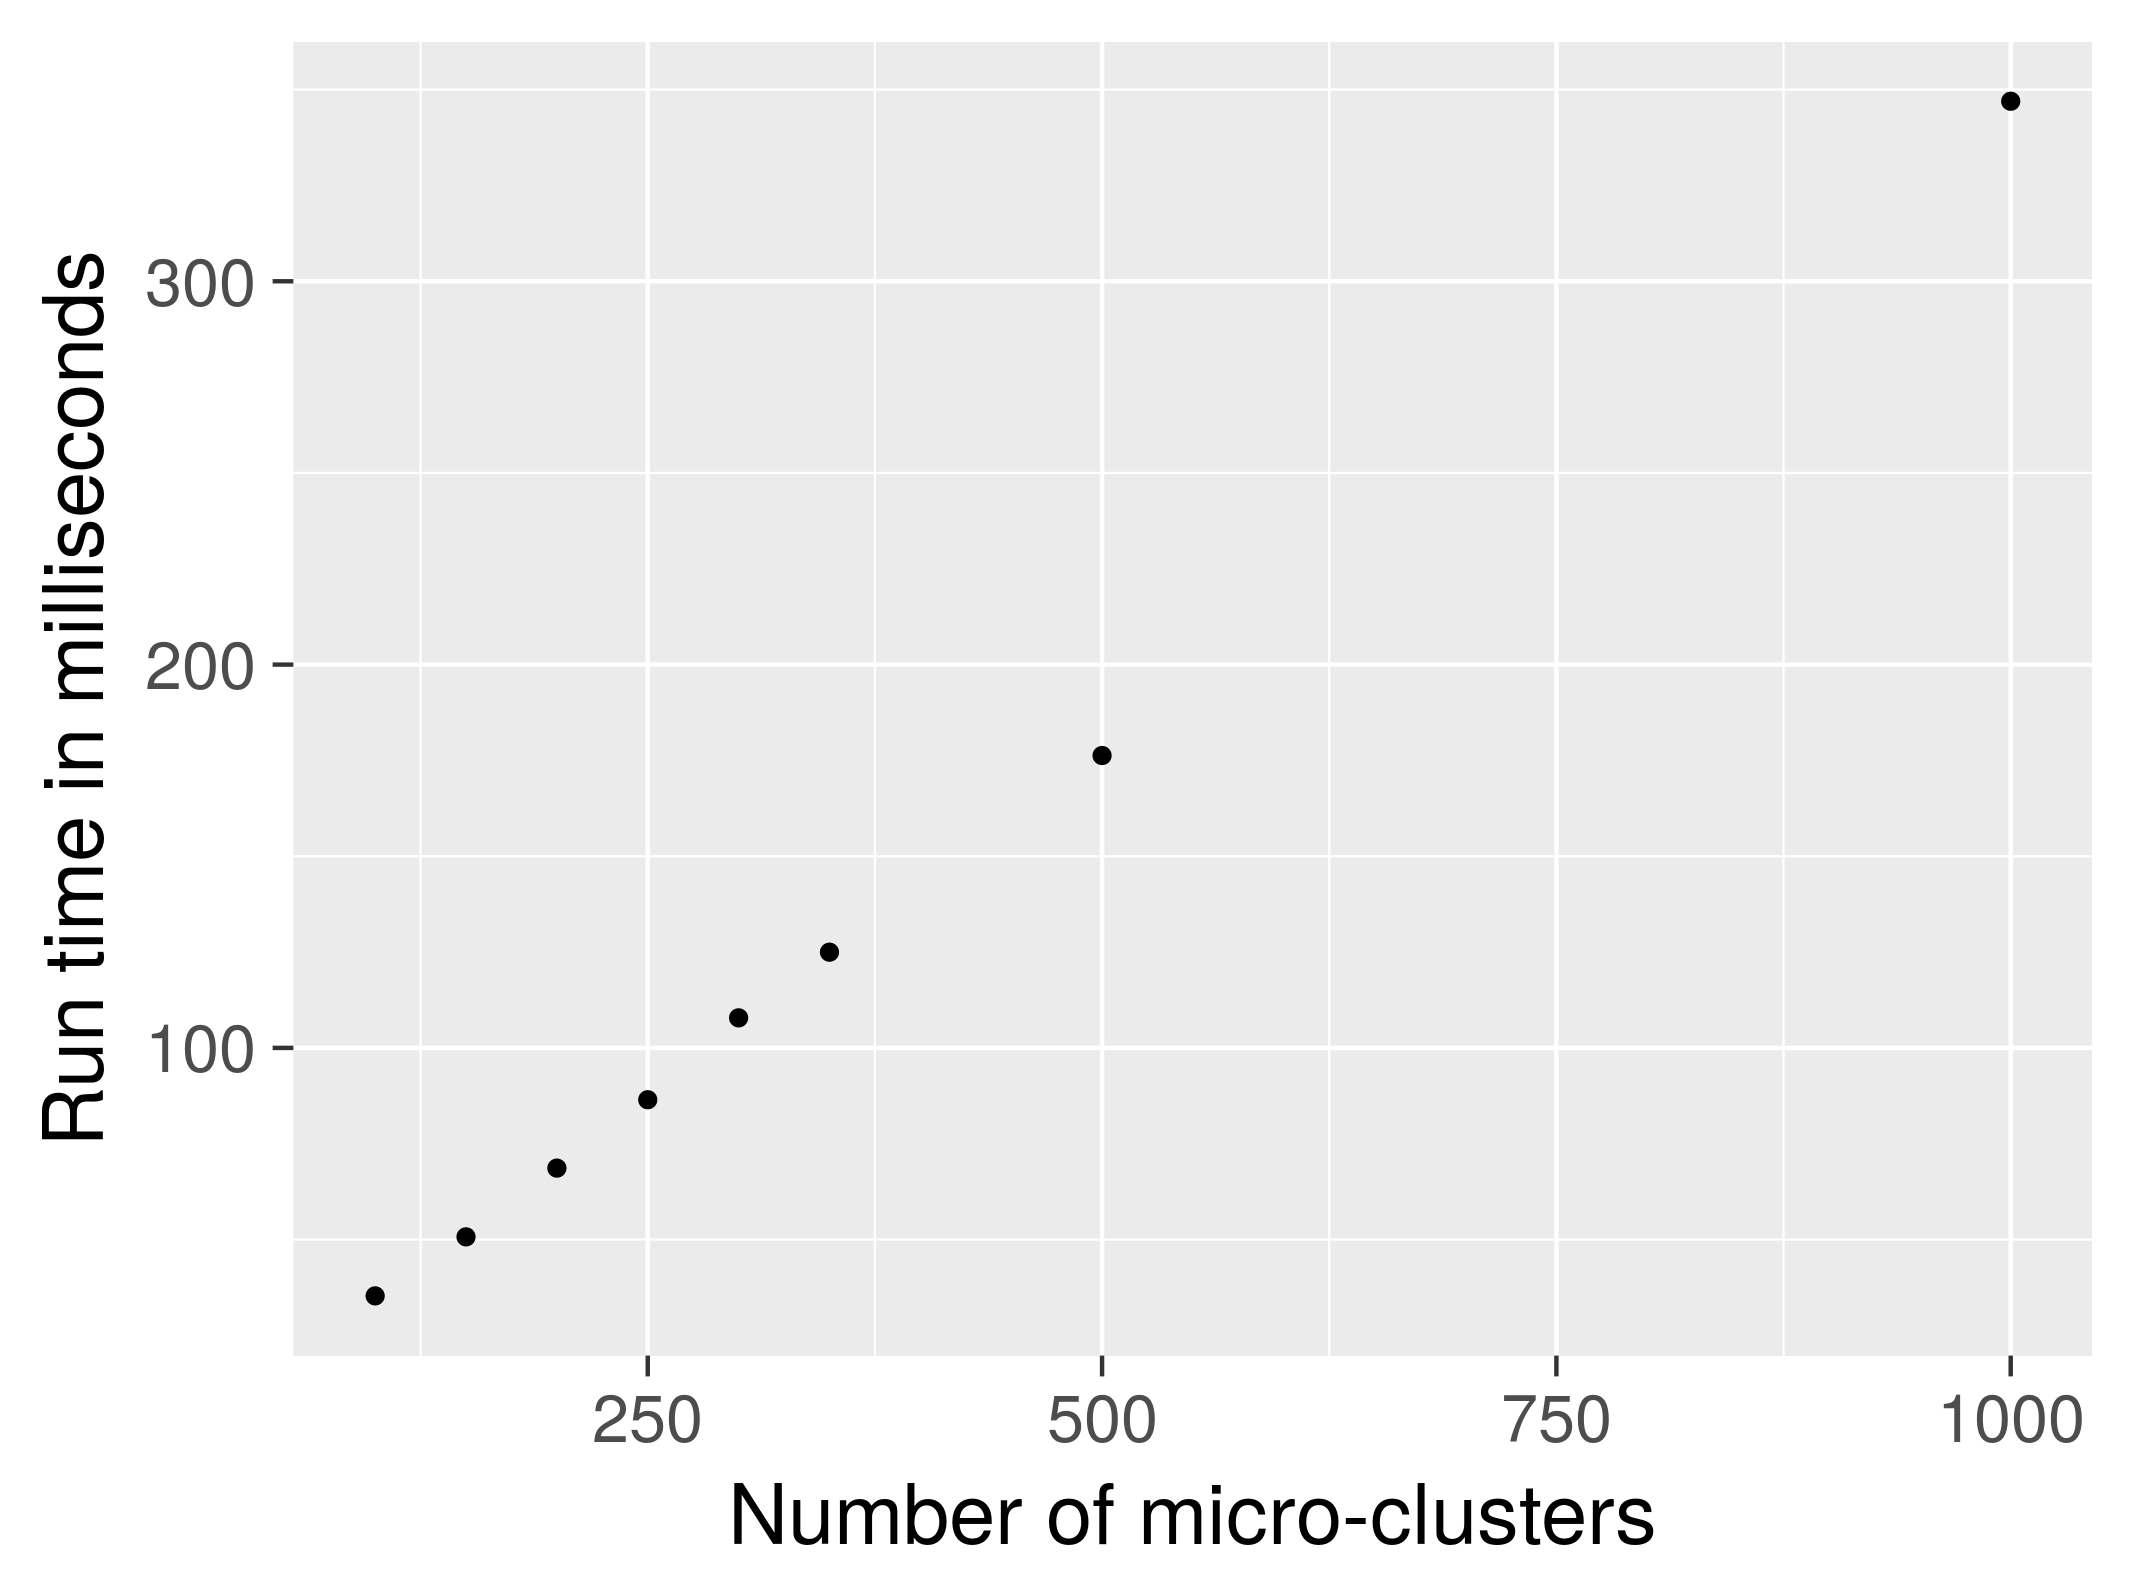
\includegraphics[width = 9cm]{efficiency_clustream.png}
  \caption{The effect of the number of micro-clusters on run time for one update.}
\label{fig:fuckYeahLinear}
\end{figure}

Each data point represents the median run time in milliseconds over 100 runs.  As we can see, the run time does increase linearly with the number of micro-clusters.

We also investigated the size of dimension of the data set on the run time of one update. The dimension of the data set had no effect on run time.  

\subsubsection{Macro-clustering stage}
 
The second stage of clustream is a macro-clustering stage, where we take the current micro-cluster feature vectors, and use these as input into global clustering algorithm. The macro-clustering step is where the general data summary is transformed into a snapshot of the true underlying clusters at that point in the stream. The $q$ micro-cluster centres $\bar{M_j},(1 \leq j \leq q$) are treated as representative points for the data stream $S$, and a standard clustering algorithm can be used to determine clusters. By using the micro-clusters to summarise the data, we can therefore perform spectral clustering on data streams.  The full algorithm is given in Algorithm \ref{alg:onlineSpec}. % The nature of this algorithm allows the user to get close to online streaming and perform spectral clustering on a summary of the whole of the data set. 

%In order to achieve this we adopt a micro-clustering type approach to quickly update a summary of the data. When an overall clustering is required, spectral clustering is performed using the centres of the micro-clusters as the input data. The micro-clusters act as a way of summarising the constantly arriving data steam whilst allowing updates to occur in a non intrusive, non-computationally difficult manner, with limited storage requirements. 

\begin{algorithm}
\caption{Spectral CluStream}
\begin{algorithmic}[1]
\REQUIRE  Data Stream $S = \{\boldsymbol{x_i} \}_{i \in \mathbb{N}}, \boldsymbol{x_i} \in \mathbb{R}^d$, number of clusters $k$, number of micro-clusters $q$, parameters $\delta$, $\tau$, $m$.
\ENSURE A $k$ way clustering of the micro-clusters $M_1, \ldots, M_q$.
\STATE Initialise the micro-clusters using k-means($x_1, \hdots x_{init},q$) and equations \eqref{eq:microcluster_def}.
\FOR {each new data point $x_i$}
 \STATE Apply CluStream update as in Algorithm \ref{alg:clustream}.
 \IF{A Macro-clustering is required}
   \STATE Perform spectral clustering on $M_1, \ldots, M_q$ with $k$ clusters.
\ENDIF
\ENDFOR

\end{algorithmic}
\label{alg:onlineSpec}
\end{algorithm}

The frequency with which the macro-clustering stage is run depends on how often the user requires a summary of the clusters. This will be determined by the nature of the application. As the macro-clustering stage is considered an offline step in CluStream \citep{Aggarwal2003}, the efficiency of the algorithm is not compromised by running the macro-clustering more frequently. 

There are a couple of possible ways to feed the micro-clusters into a spectral clustering algorithm (step 5 of Algorithm \ref{alg:onlineSpec}). Two of the options suggested in \cite{Zhang1996a} listed here. 

\begin{enumerate}
\item Calculate the centre of each micro-cluster $\bar{M_j}$ and use it as an object to be clustered by the macro-clustering algorithm.
\item Do the same as before, but weighting each micro-cluster centre $\bar{M_j}$ proportionally to $n_j$, the number of points assigned to that micro-cluster, so that micro-clusters with more objects will have more influence on the final clustering.
\end{enumerate}

No guidance is given in \cite{Zhang1996a} to how these two different approaches might affect the final clustering result. Next, in Section \ref{sec:weighting} we describe how to weight the micro-cluster centers. Later in Section \ref{sec:clustream_exp} we will analyse the performance of both unweighted and weighted online spectral clustering.

\subsection{Weighting the Micro-Clusters}
\label{sec:weighting}

In this section, we discuss how to create a weighted affinity matrix, look at the effect this has on the Laplacians and note a spectral link between weighting in this manner and using larger affinity consisting of repeated points.
Weighting the micro-clusters is suggested in \cite{Zhang1996a} but why might it be beneficial to weight the micro-clusters?  The first thing to note is that the number of data points assigned to micro-clusters is not uniform across the micro-clusters, and this distribution will change as the stream progresses.  For example, Figure \ref{fig:hist1} shows a histogram of the number of points assigned to micro-clusters at the start of a data stream, Figure \ref{fig:hist2} shows the middle of the stream, and Figure \ref{fig:hist3} shows the end of the stream. We can see that the distribution is not uniform. Therefore some information is contained in the number of points assigned to a micro-cluster. 

\begin{figure}[h!]
  \centering
  \begin{subfigure}{0.32\textwidth}
    \centering
    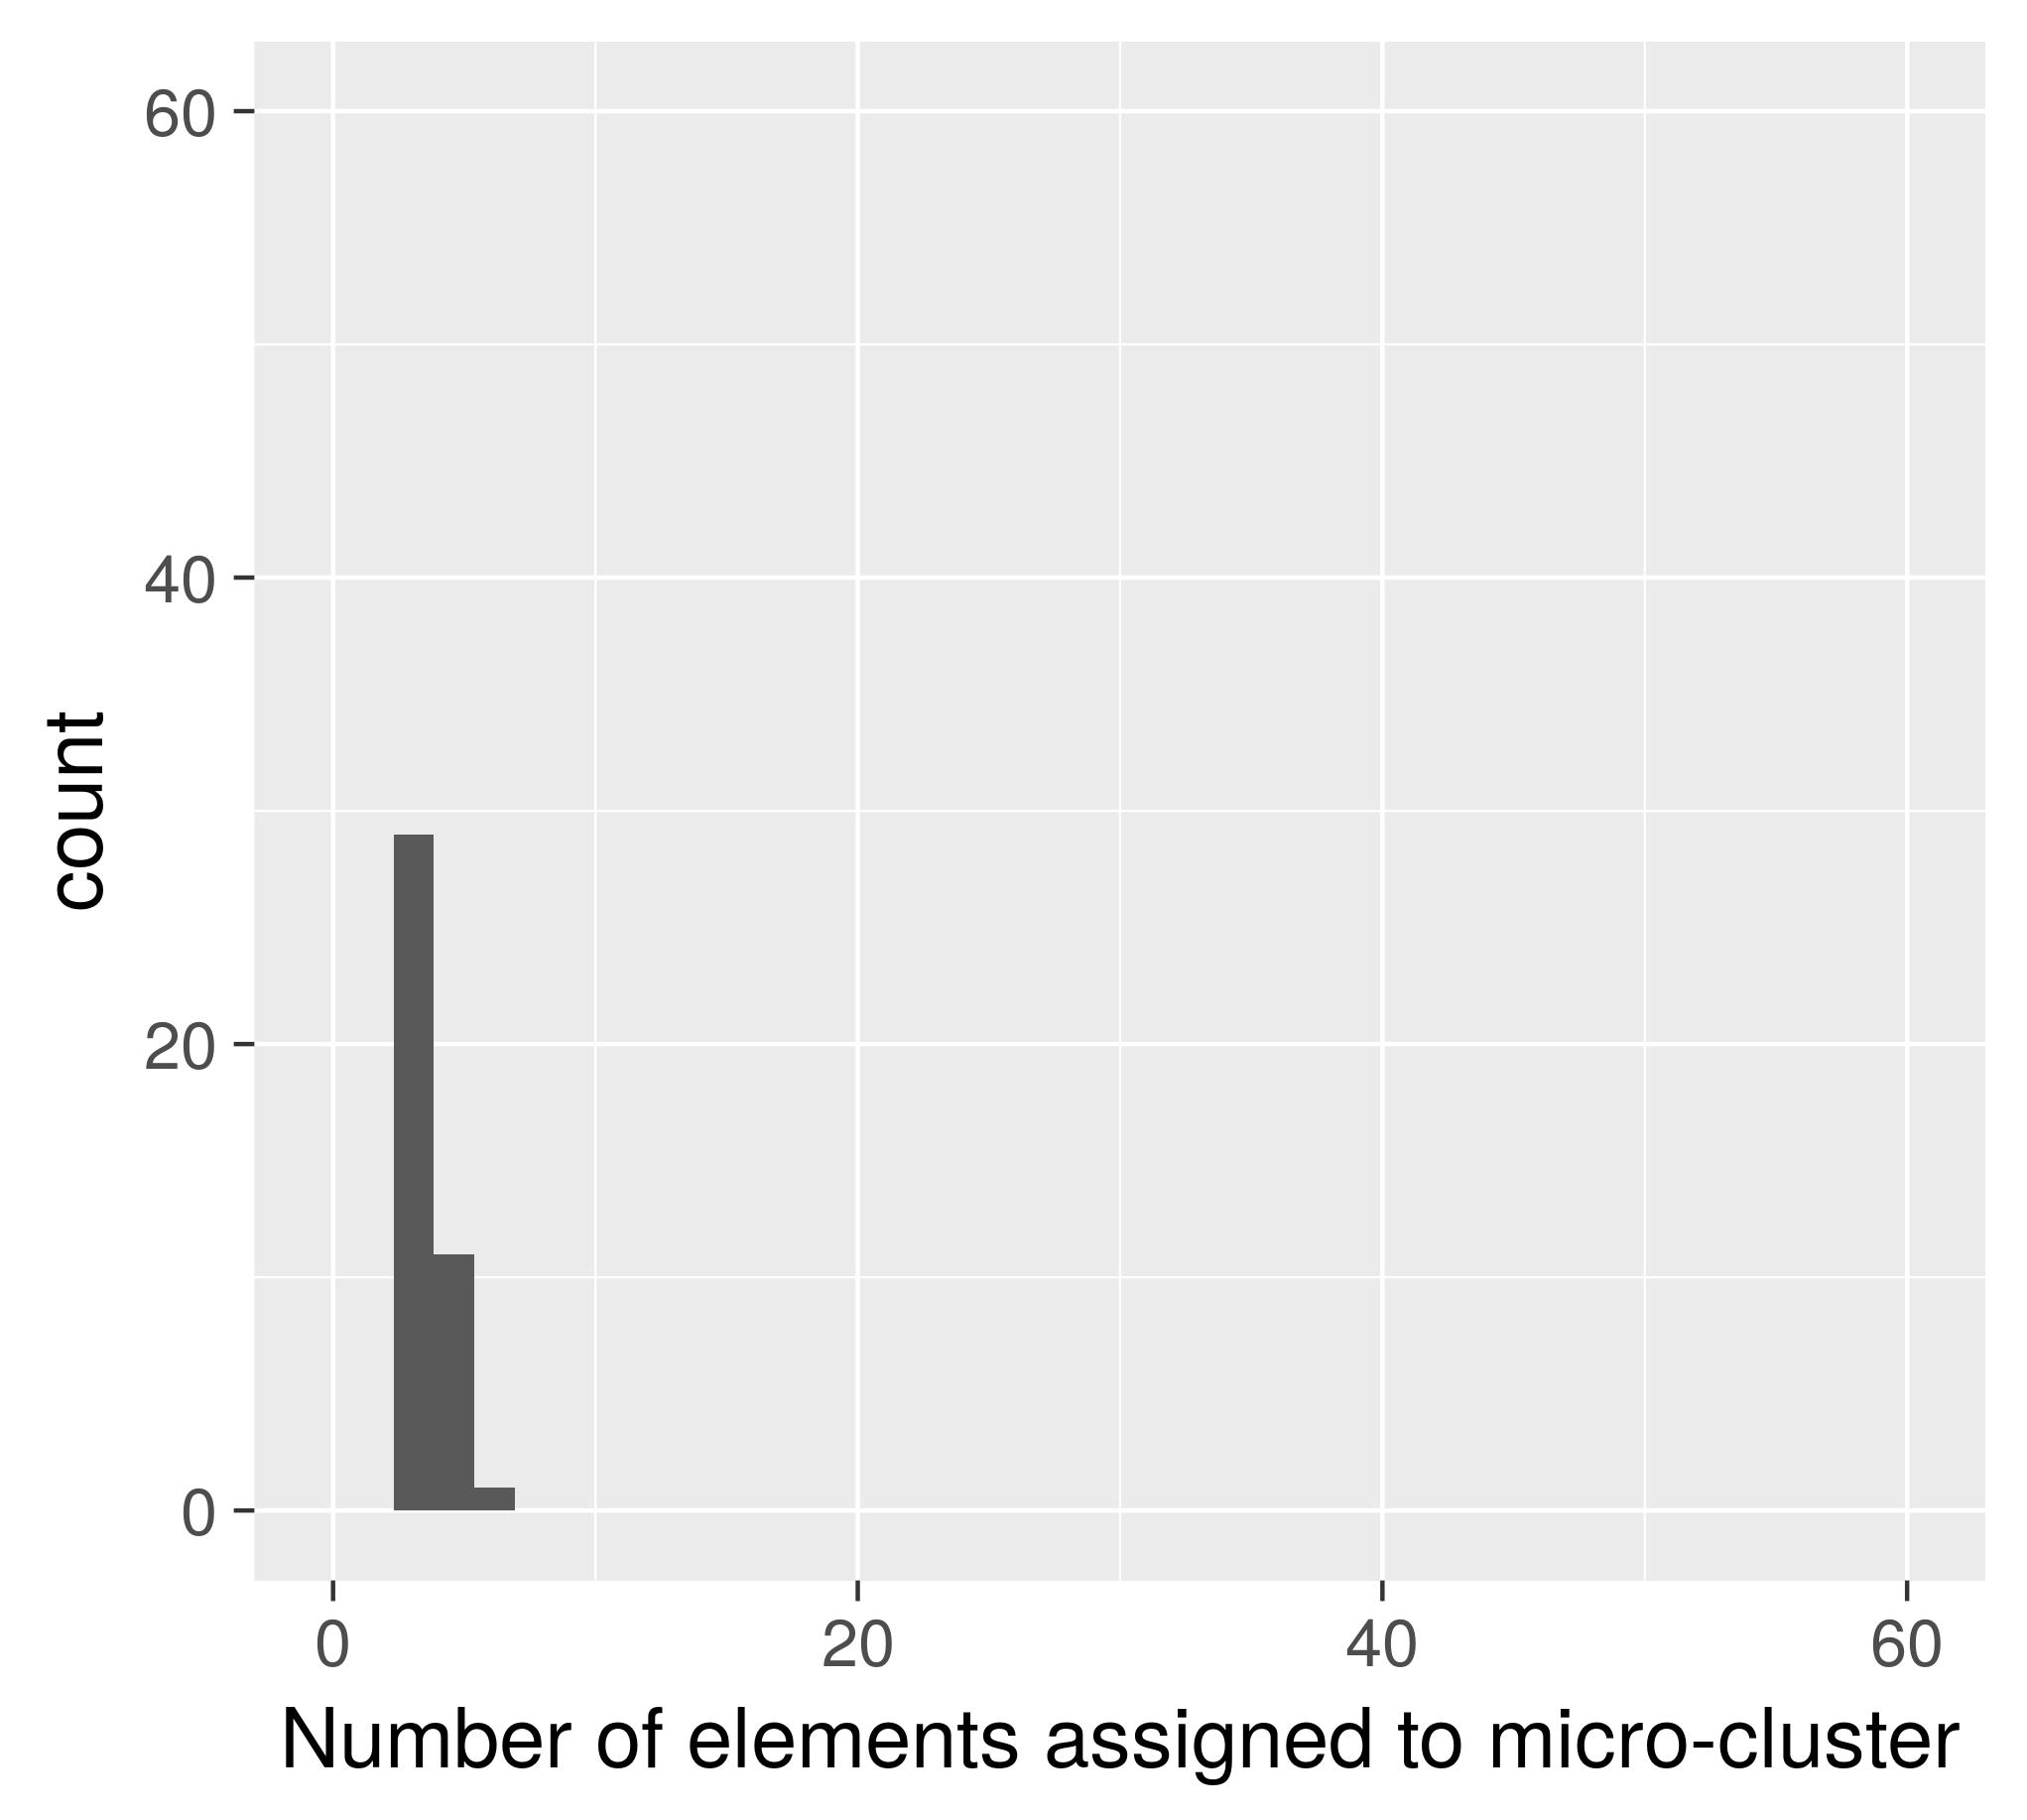
\includegraphics[width = \textwidth]{microcluster_histograms/s_set_1_hist_t_501.png}
    \caption{Start of the stream.}
  \label{fig:hist1}
  \end{subfigure}
  \begin{subfigure}{0.32\textwidth}
    \centering
    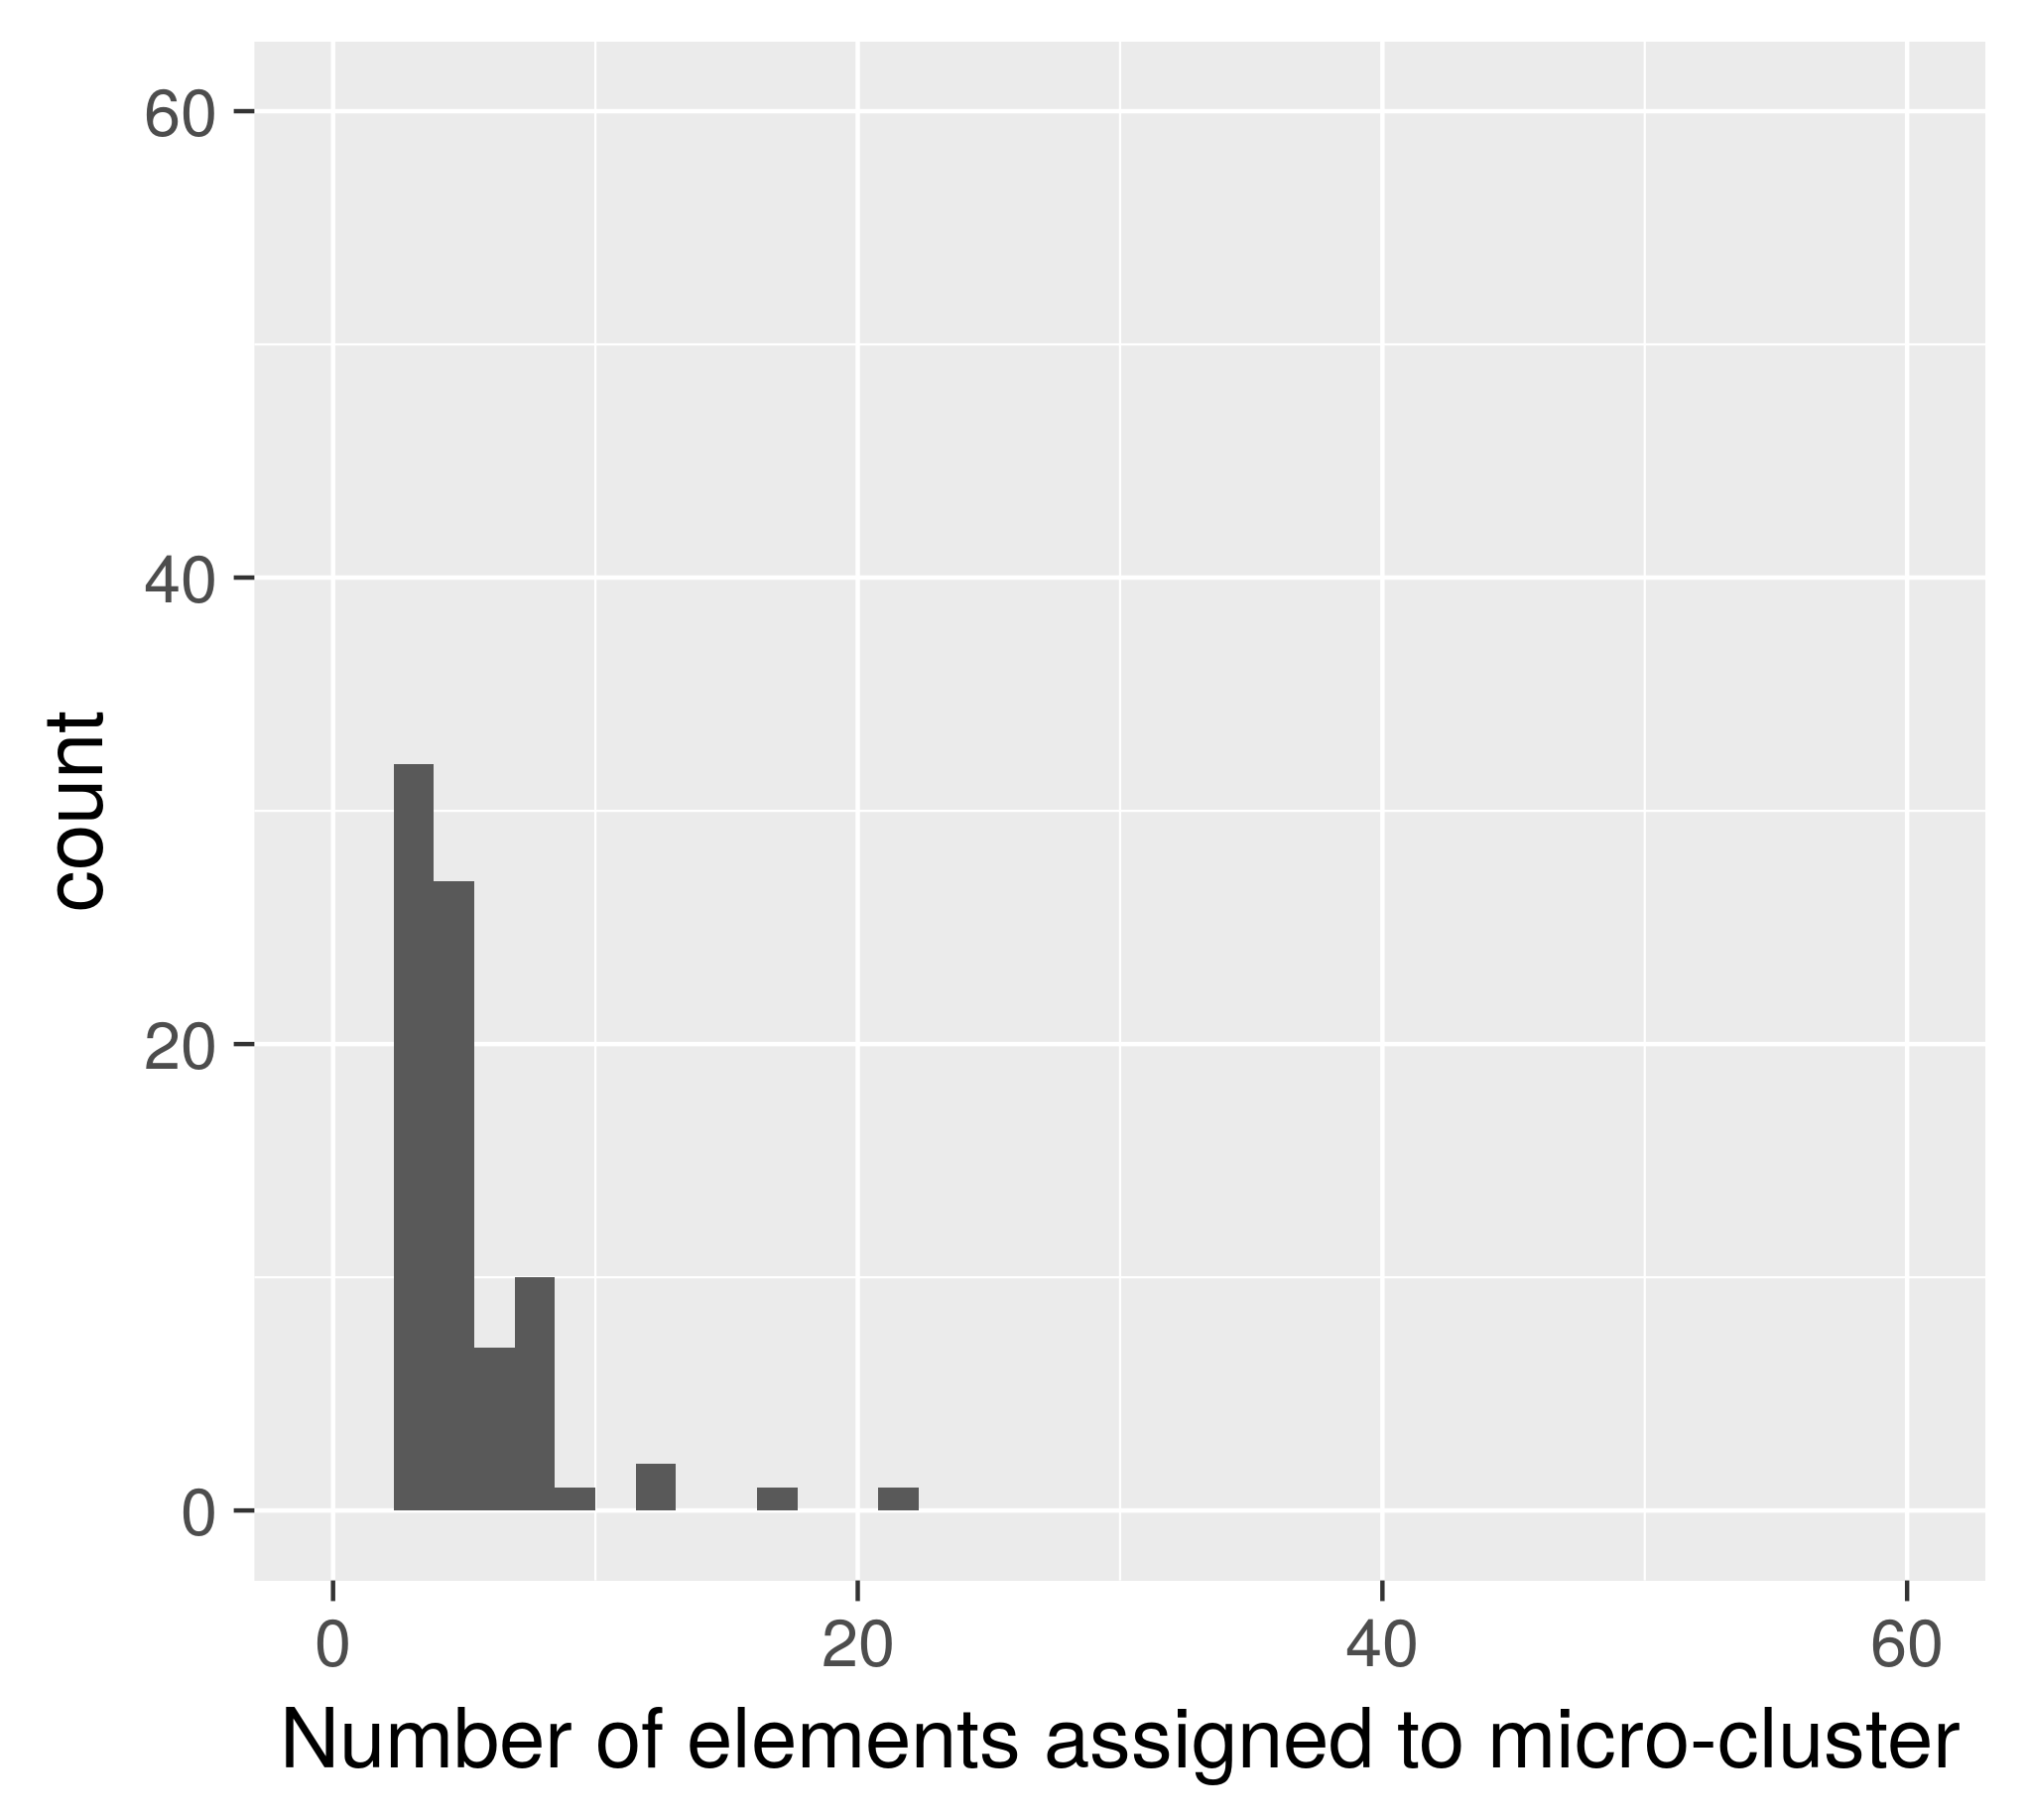
\includegraphics[width = \textwidth]{microcluster_histograms/s_set_1_hist_t_1250.png}
  \caption{Middle of the stream.}
  \label{fig:hist2}
  \end{subfigure}
\begin{subfigure}{0.32\textwidth}
    \centering
    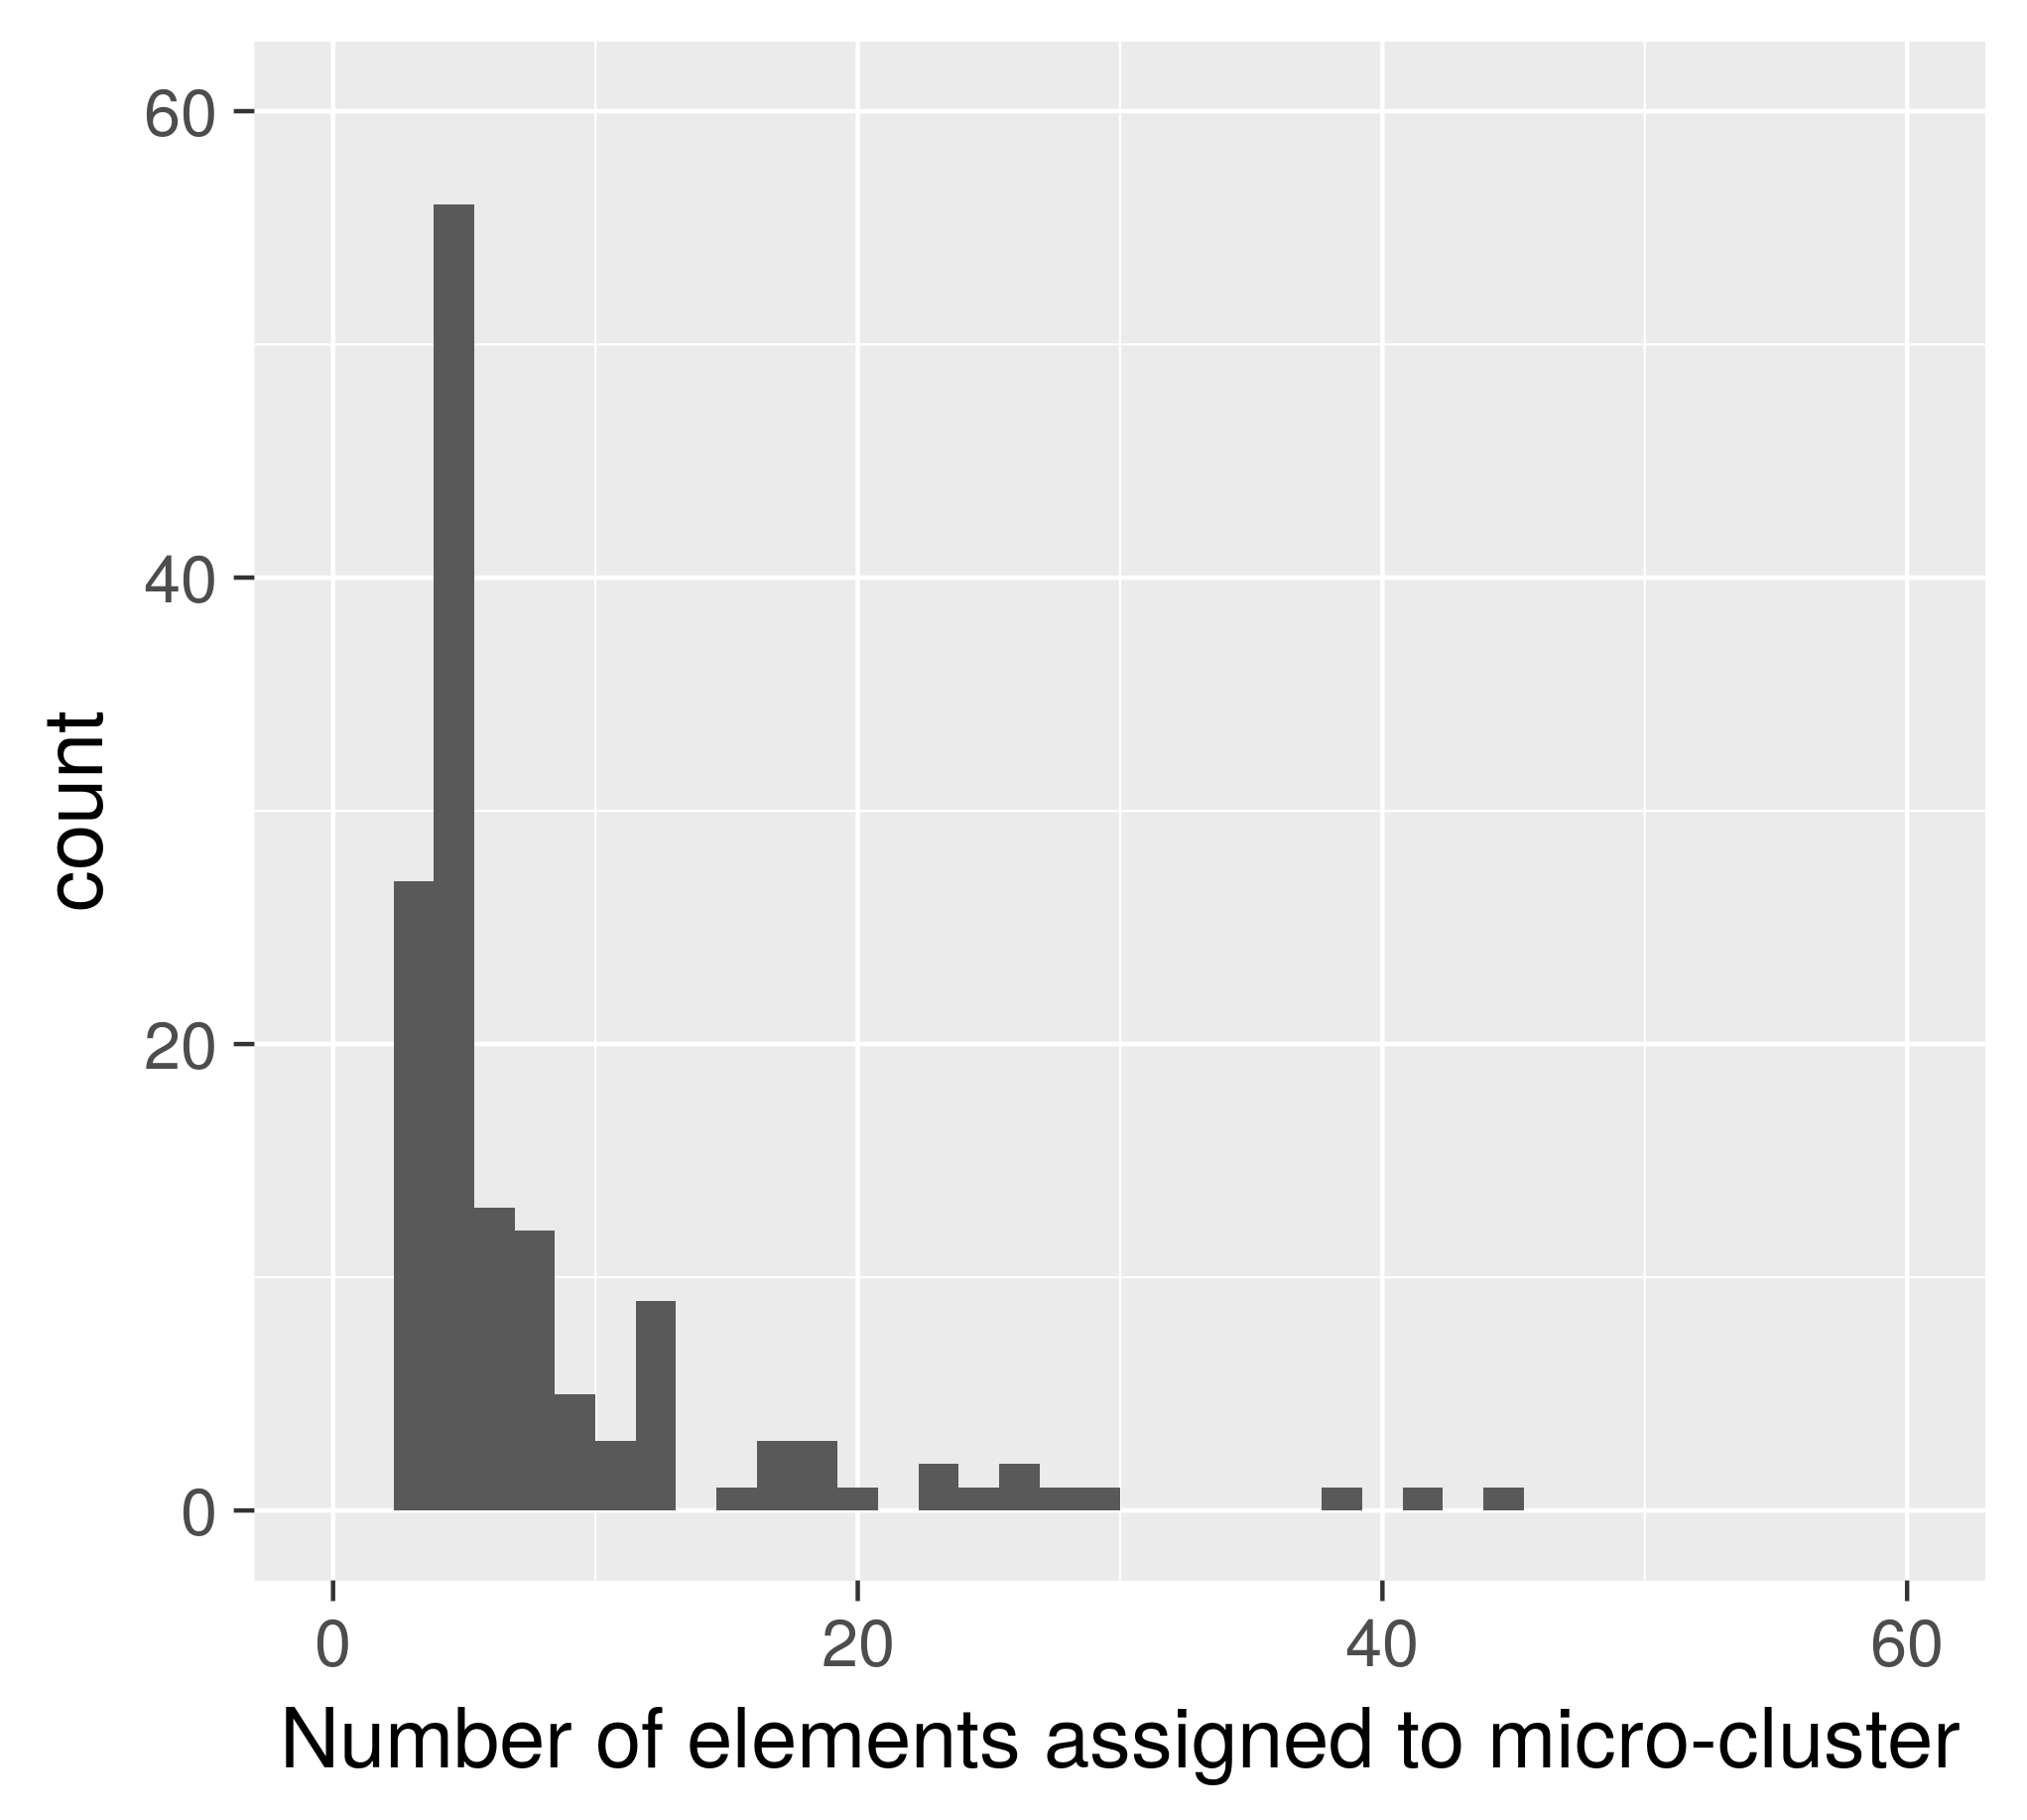
\includegraphics[width = \textwidth]{microcluster_histograms/s_set_1_hist_t_2000.png}
  \caption{End of the stream.}
  \label{fig:hist3}
  \end{subfigure}
    \caption{Histograms showing the number of points assigned to micro-clusters.}
  \label{fig:microHist}
\end{figure}

Secondly, imagine the scenario pictured in Figure \ref{fig:motivate_weighting} where we have two clusters, one much more dense that then other.  In the example, many micro-clusters are used to represent the  cluster on the right, although each micro-cluster only has a few data points assigned to it. The more dense cluster in the bottom left of the plot has only 3 micro-clusters representing it, but each micro-cluster has hundreds of data points assigned to it.   Weighting by the number of points assigned to a micro-cluster may help balance out this scenario for the spectral clustering stage. 

\begin{figure}[h]
  \centering
  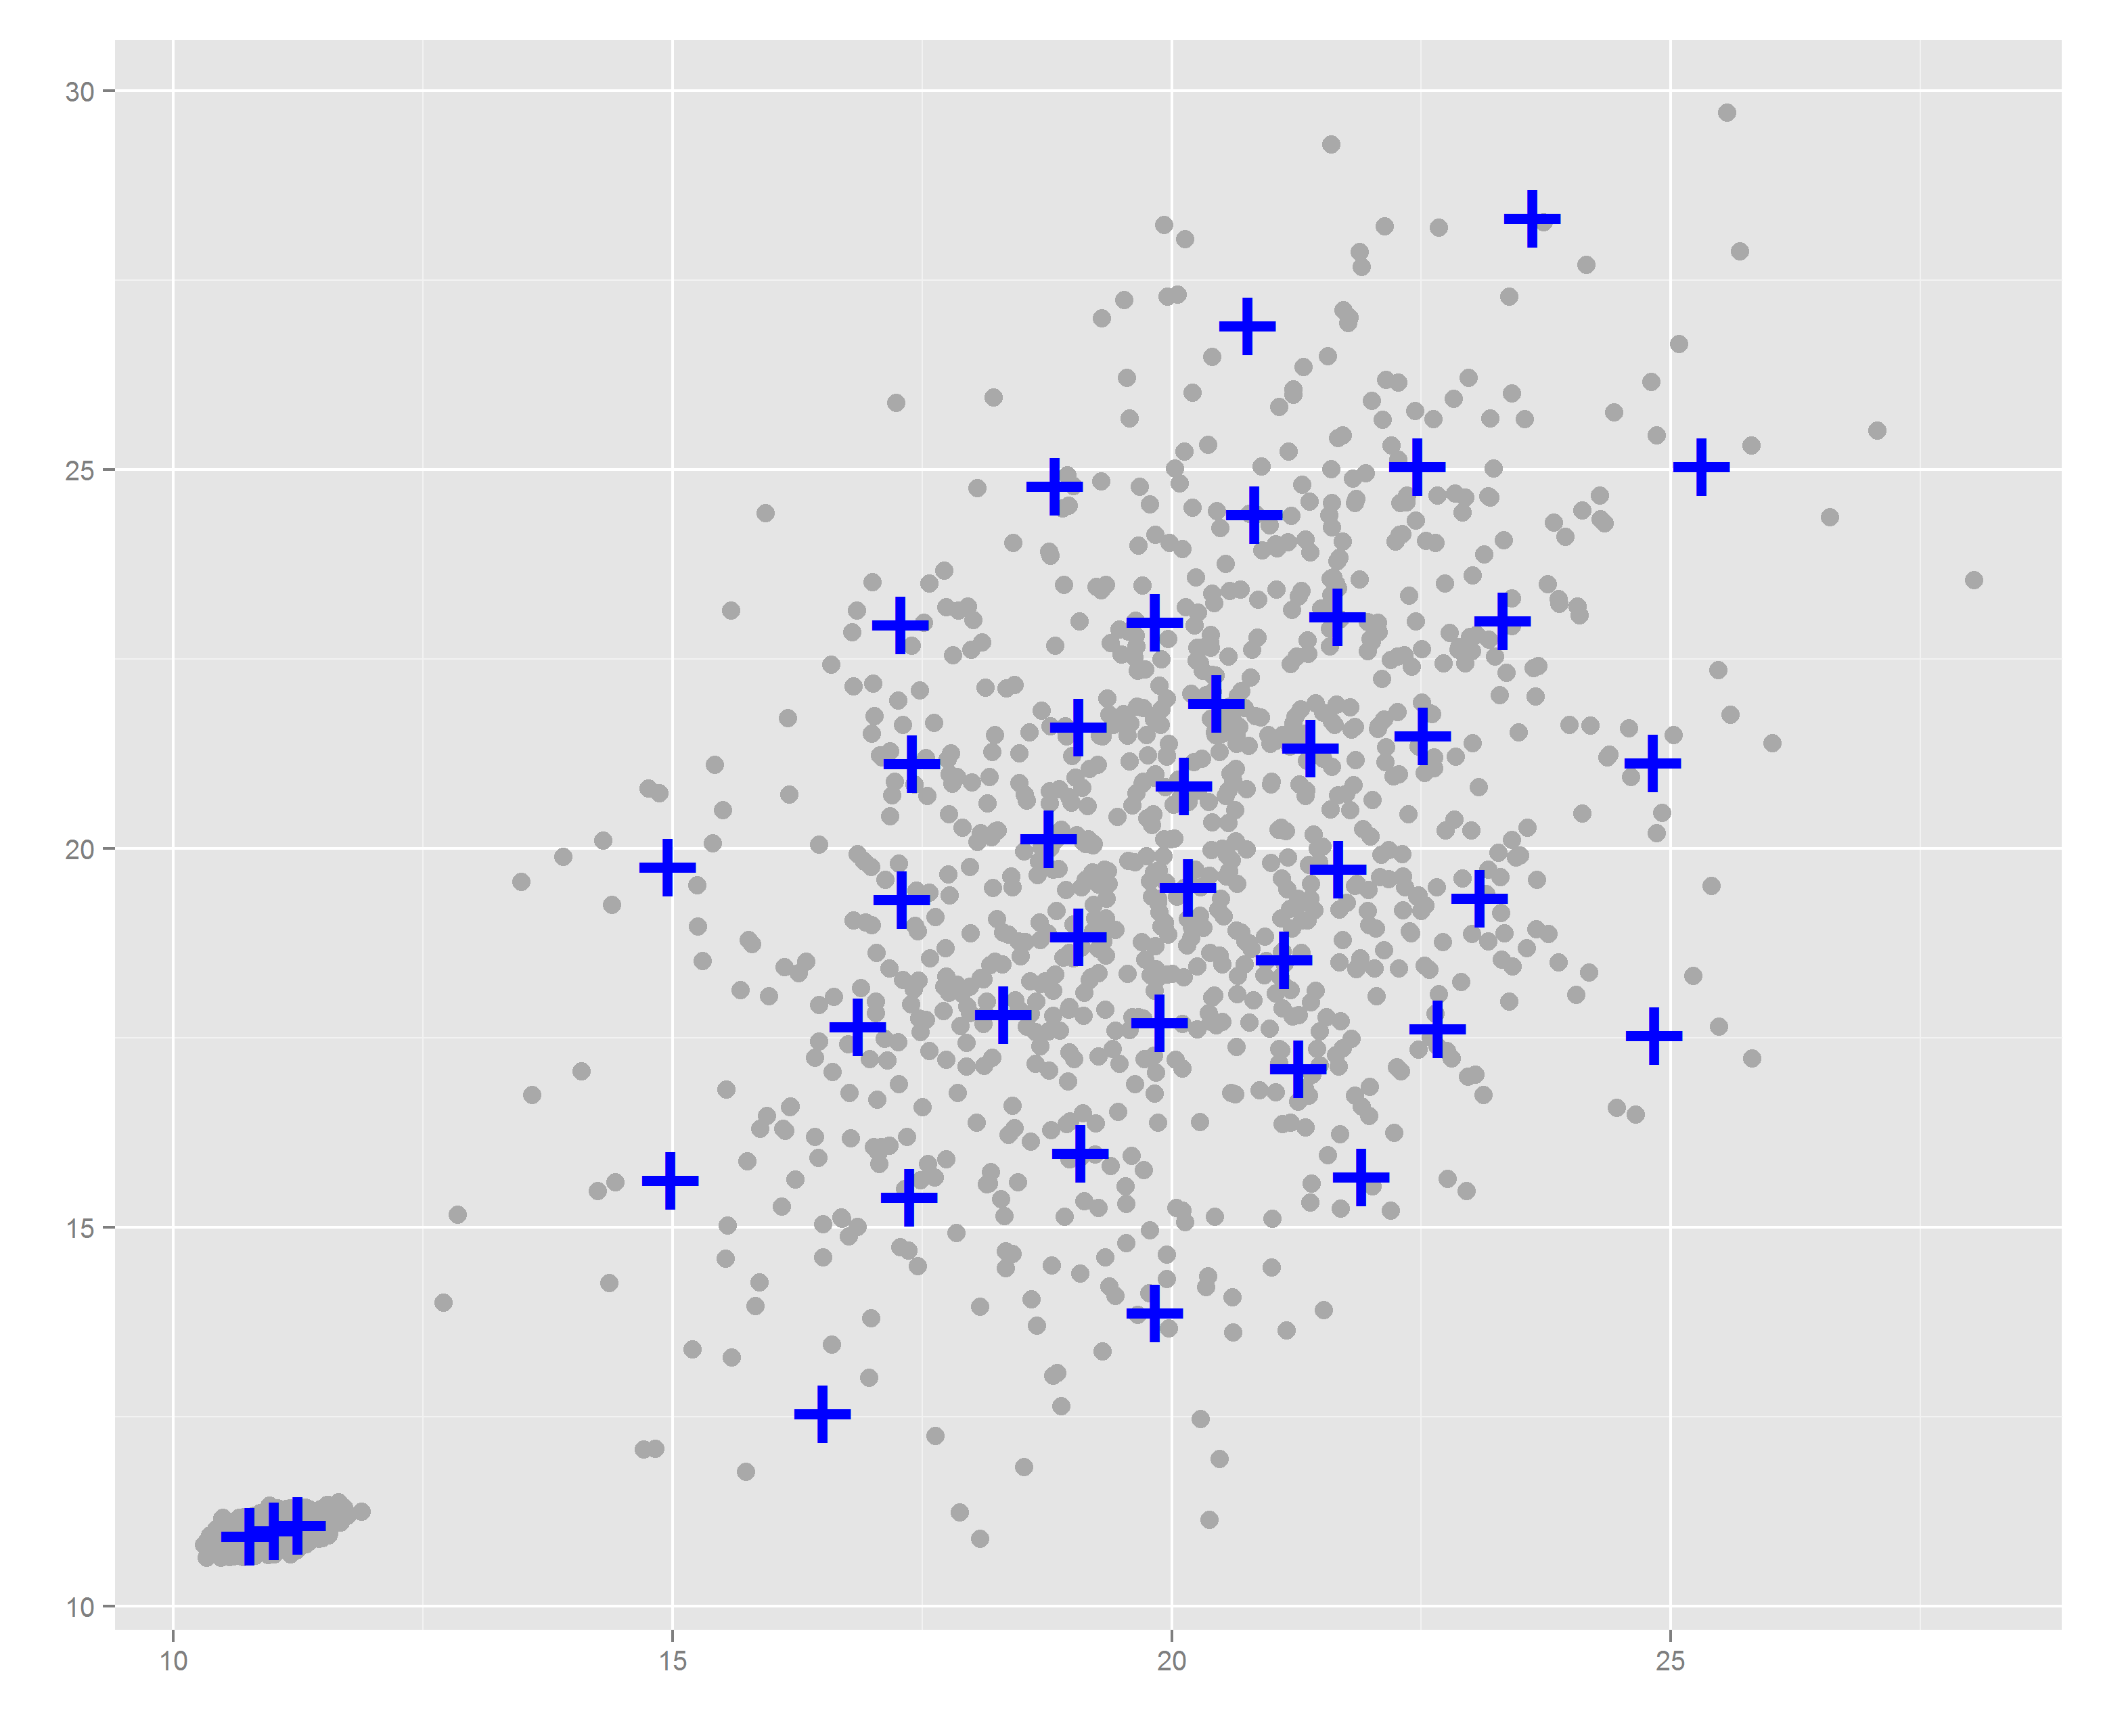
\includegraphics[width = 8cm]{motivate_weighting.png}
  \caption{Possible micro-cluster  locations in a toy example.}
\label{fig:motivate_weighting}
\end{figure}

In order to weight the micro-clusters, we simply construct an affinity matrix as described. Let $W \in \mathbb{R}^{q \times q}$ be the affinity matrix of the micro-cluster centres with $i,j$-th element equal to the similarity between micro-cluster $M_i$ and $M_j$, 

\[ W_{i,j} = \exp \left(- \frac{\| \bar{M_i} - \bar{M_j}\|^2}{2 \sigma^2} \right), \quad i, j = 1, \ldots, q. \]
\\
Define the \textit{weighted affinity matrix} to be $\tilde{W} \in \mathbb{R}^{q \times q}$ where $ \tilde{W_{ij}} = n_in_jW_{ij}$. We can see that $\tilde{W}$ is a valid affinity matrix since it is symmetric with non-negative entries. If we wish to have $\tilde{W}_{ij} \leq 1$ then simply divide $\tilde{W}$ by $\max_i n_i^2$, but this makes no difference to the spectral decomposition \citep{Luxburg2008}. 

There exists a link between the spectral decomposition of  the Laplacian generated by $\tilde{W}$ and the Laplacian arising from a data set of repeated points, which we define as follows.  Let $W^* \in \mathbb{R}^{n \times n}$ be the repeated affinity matrix with the micro-cluster centres repeated based on the number of points assigned to them. Assume that the columns (and therefore rows) of $W^*$ are ordered such that the first $n_1$ are associated with the data assigned to micro-cluster 1, which has size $n_1$ and the next $n_2$ with those assigned to micro-cluster 2, and so on. Let $D, \tilde{D}, D^{*},$ be the corresponding degree matrices and $L, \tilde{L}, L^{*}$ be the corresponding normalised symmetric Laplacians.

Let us consider the affinity and Laplacian matrices more closely for a very simple case. Assume that we have two micro-clusters, $M_1$ and $M_2$,  which have $n_1$ and $n_2$ points assigned to them respectively. Let the similarity between the two micro-cluster centres be $s$, and assume that we are using the standard Gaussian kernel to generate affinity matrices, so therefore the diagonal elements will be equal to 1. The affinity, degree and Laplacian matrices ($W$, $D$ and $L$) for the two micro-cluster centres are given in equation \eqref{eq:example_centers}.

\begin{equation}
  \label{eq:example_centers}
 W = \left(
  \begin{array}{cc}
    1 & s \\
    s & 1
  \end{array} \right), \quad
%
 D = \left(
  \begin{array}{cc}
    1+s & 0 \\
    0 & 1+s
  \end{array} \right), \quad
%
 L = \left(
  \begin{array}{cc}
    \frac{1}{1+s} & \frac{s}{1+s} \\
    \frac{s}{1+s} & \frac{1}{1+s} 
  \end{array} \right). 
\end{equation}
\\
In order to create a weighted version of the affinity matrix, we simply multiply through by $n_1$ and $n_2$. The weighted affinity matrix $\tilde{W}$ and related degree and Laplacians ($\tilde{D}$ and $\tilde{L}$) are given in equation \eqref{eq:example_weighted}.% We can see how this is incorporated into the Laplacian. Note that we are working with the Symmetric Normalised Laplacian. In order to weight in this manner for the unnormalised Laplacian a scaling of the diagonal matrix is would be required  \citep{Luxburg2008}.
\\
\begin{equation}
\begin{gathered}
 \tilde{W} = \left(
  \begin{array}{cc}
    n_1^2 & sn_1n_2 \\
    sn_1n_2 & n_2^2
  \end{array} \right) , \quad 
%
 \tilde{D} = \left(
  \begin{array}{cc}
    n_1^2 + sn_1n_2 & 0 \\
    0 & n_2^2 + sn_1n_2
  \end{array} \right), \\ \\ 
 \tilde{L} = \left(
  \begin{array}{cc}
   \frac{n_1^2}{n_1^2+sn_1n_2} & \frac{sn_1n_2}{\sqrt{(n_1^2+sn_1n_2)(n_2^2+sn_1n_2)}} \\
   \frac{sn_1n_2}{\sqrt{(n_1^2+sn_1n_2)(n_2^2+sn_1n_2)}} &  \frac{n_2^2}{n_2^2+sn_1n_2}
  \end{array} \right). \\
\end{gathered} \label{eq:example_weighted} 
\end{equation}
\\
Finally we observe the construction of the repeated affinity matrix given in equation \eqref{eq:example_repeated}. Here the block nature in $W^*$, $D^*$ and $L^*$ is clear. The first $n_1$ rows of $W^*$ relate to the centre of micro-cluster 1, and the bottom $n_2$ rows relate to the centre of micro-cluster 2.

\begin{equation}
\begin{gathered}
  W^* = \left(
  \begin{array}{cccccc}
    1 & \hdots & 1 & s & \hdots & s \\
    \vdots & \ddots & \vdots & \vdots & \ddots & \vdots \\
    1 & \hdots & 1 & s & \hdots & s \\
   s & \hdots & s & 1 & \hdots & 1 \\
    \vdots & \ddots & \vdots & \vdots & \ddots & \vdots \\
    s & \hdots & s & 1 & \hdots & 1 
  \end{array} \right) , \quad 
%
 D^* = \left(
  \begin{array}{cccccc}
    \star & 0 & 0 & 0 & \hdots & 0 \\
    0 & \ddots & 0 & \vdots & \ddots & \vdots \\
    0 & 0 & \star & 0 & \hdots & 0 \\
   0 & \hdots & 0 & \bigtriangleup & 0 & 0 \\
    \vdots & \ddots & \vdots & 0 & \ddots & 0 \\
    0 & \hdots & 0 & 0 & 0 & \bigtriangleup 
  \end{array} \right), \\
%
 L^* = \left(
  \begin{array}{cccccc}
    \frac{1}{\star} & \hdots & \frac{1}{\star} & \frac{s}{\sqrt{\star \bigtriangleup}} & \hdots & \frac{s}{\sqrt{\star \bigtriangleup}} \\
    \vdots & \ddots & \vdots & \vdots & \ddots & \vdots \\
    \frac{1}{\star} & \hdots & \frac{1}{\star} & \frac{s}{\sqrt{\star \bigtriangleup}} & \hdots & \frac{s}{\sqrt{\star \bigtriangleup}} \\
   \frac{s}{\sqrt{\star \bigtriangleup}} & \hdots & \frac{s}{\sqrt{\star \bigtriangleup}} & \frac{1}{\bigtriangleup}  & \hdots &  \frac{1}{\bigtriangleup} \\
    \vdots & \ddots & \vdots & \vdots & \ddots & \vdots \\
    \frac{s}{\sqrt{\star \bigtriangleup}} & \hdots & \frac{s}{\sqrt{\star \bigtriangleup}} & \frac{1}{\bigtriangleup}  & \hdots &  \frac{1}{\bigtriangleup} 
  \end{array} \right), 
\\
\text{where } \star = n_1 + n_2s \text{ and } \bigtriangleup = n_1s + n_2. 
\end{gathered} \label{eq:example_repeated}
\end{equation}

If we evaluate these expressions for a particular numerical case, we can see how the spectral decomposition of the matrices $\tilde{L}$ and $L^*$ are linked.
Let $s = 0.5$, $n_1 = 3$, $n_2 = 2$. The 2nd smallest eigenvector of $L^*$ is 

\begin{equation}
  \label{eq:e2*}
   e_2^* = \left[ 
\begin{array}{ccccc}
  -0.350& -0.350& -0.350& 0.562& 0.562  
\end{array} \right].
\end{equation}

The 2nd smallest eigenvector of $\tilde{L}$ is 

\begin{equation}
  \label{eq:e2}
   \tilde{e}_2 = \left[ 
\begin{array}{cc}
  0.607 & -0.795 \\
\end{array} \right] .
\end{equation}

If we expand the eigenvector $\tilde{e}_2$ by expanding it's elements and block dividing by $\sqrt{n_1}$ and $\sqrt{n_2}$ respectively, we get the following, 
\begin{equation}
  \label{eq:e_repeat}
   \left[ \; \overbrace{\frac{0.607}{\sqrt{3}} \; \frac{0.607}{\sqrt{3}} \; \frac{0.607}{\sqrt{3}}}^{n_1} \; \overbrace{\frac{-0.795}{\sqrt{2}} \; \frac{-0.795}{\sqrt{2}}}^{n_2} \; \right] 
=  \left[ 
\begin{array}{ccccc}
0.350& 0.350& 0.350 & -0.562& -0.562  
\end{array} \right] .
\end{equation}

We can see that the right hand vector in equation \eqref{eq:e_repeat} is the negative of the 2nd smallest eigenvector of $L^*$, $e_2^* $ given in equation \eqref{eq:e2*}. %This result 


In fact, we have seen empirically that the expanded repeated eigenvector of the weighted Laplacian is always either equal to $e_k^*$ or $-e_k^*$ for all $k$. This means that the partition generated by performing spectral clustering on the weighted micro-cluster centers will be the same as the partition generated by performing spectral clustering on a set of repeated micro-cluster centers.

Proposition \ref{prop:dave} proves that the second smallest eigenvectors of spectral decomposition of $L^*$ and $\tilde{L}$ are linked in this way.

%Generally, the spectral decomposition of $L^*$ and $\tilde{L}$ are linked in this way, and therefore the partition generated by performing spectral clustering on the weighted micro-cluster centers will be the same as the partition generated by performing spectral clustering on a set of repeated micro-cluster centers. We do not show the full proof for this here but prove that the second smallest eigenvectors are linked in this way. 

\begin{proposition}
\label{prop:dave}
Let $L$ be a symmetric Laplacian matrix. Define $\tilde{L}$ and $L^*$ to be the corresponding weighted and expanded Laplacians respectively. Let $\tilde{u}$ be the second smallest eigenvector of  $\tilde{L}$.  Then $u^*$ is the second smallest eigenvector of $L^*$, where $u^*$ is defined as $u^* =  \left( \overbrace{\frac{\tilde{u}_1}{\sqrt{n_1}}, \; \frac{\tilde{u}_1}{\sqrt{n_1}}, \; \frac{\tilde{u}_1}{\sqrt{n_1}}}^{n_1}, \; \hdots, \overbrace{\frac{\tilde{u}_k}{\sqrt{n_k}}, \; \frac{\tilde{u}_k}{\sqrt{n_k}}}^{n_k} \right)$. 
\end{proposition}

\begin{proof}
We wish to show that $u^*$ is the second smallest eigenvector of $L^*$.  First we will show that $u^*$ is an eigenvector of $L^*$ which is orthogonal to the smallest eigenvector of $L^*$. Then we will show by proof by contradiction that $u^*$ must be the second smallest eigenvector of $L^*$. 
%We can see that $\|u^*\|^2 = \sum_{i = 1}^{n}(u_i^*)^2 = \sum_{i=1}^{k}n_i \cdot \frac{\tilde{u}_i^2}{n_i} = \sum_{i = 1}^{k} \tilde{u}^2_i = 1$. 
\newpage
i) $ \|u^*\| = 1. $

\begin{align*}
 \|u^*\|^2 &= \sum_{i=1}^{n}u^{* 2}_i, \\
&= \sum_{i = 1}^{k}n_i \frac{\tilde{u}_i^2}{n_i}, \\
&= \sum_{i=1}^{k}\tilde{u}_i^2 = 1, 
\end{align*}
since $\tilde{u}$ is an eigenvector. Therefore $\|u^*\| = 1$. 

ii)  $u^* \perp D^{* 1/2} \mathds{1}$.

\begin{align*}
 \sum_{i=1}^nu^*_i D_{ii}^{* 1/2} &= \sum_{i=1}^k n_i \frac{\tilde{u}_i}{\sqrt{n_i}} \frac{\tilde{D}^{1/2}_{ii}}{\sqrt{n_i}}, \\
&= \sum_{i=1}^k \tilde{u}_i \tilde{D}^{1/2}_{ii} = 0,
\end{align*}
\noindent since $\tilde{u} \perp \tilde{D}^{1/2} \mathds{1}$, therefore $u^* \perp D^{* 1/2} \mathds{1}.$ 

iii) $u^{*\top} L^* u^* = \tilde{u}^{\top} \tilde{L} \tilde{u}.$

\noindent First we state the general property given in \cite{Luxburg2008} for the normalised Laplacian. For every $f \in  \mathbb{R}^n$ we have,
\begin{equation}
  \label{eq:luxburg_vectors}
  f^{\prime}  L f = \frac{1}{2} \sum_{i,j=1}^n w_{ij} \left( \frac{f_i}{\sqrt{d_i}} - \frac{f_j}{\sqrt{d_j}}  \right)^2.
\end{equation}

\noindent Using this property, 
\begin{align*}
  \tilde{u}^{\top} \tilde{L} \tilde{u} &= \frac{1}{2} \sum_{i = 1}^k \sum_{j = 1}^k \left( \frac{\tilde{u}_i}{\sqrt{\tilde{D}_{ii \phantom{j}}}} - \frac{\tilde{u}_j}{\sqrt{\tilde{D}_{jj}}}  \right)^2 \tilde{W}_{ij}, \\
 &= \frac{1}{2} \sum_{i = 1}^k \sum_{j = 1}^k \left( \frac{\tilde{u}_i / \sqrt{n_i}}{\sqrt{D_{ii}}} - \frac{\tilde{u}_j / \sqrt{n_j}}{\sqrt{D_{jj}}} \right)^2 n_i n_j  W_{ij},
  %&= \frac{1}{2} \sum_{i = 1}^k \sum_{j = 1}^k \left( \frac{\tilde{u}_i}{\sqrt{\sum_{l=1}^kn_ln_iA^{\prime}_{ij}}} - \frac{\tilde{u}_j}{\sqrt{\sum_{l=1}^kn_ln_jA^{\prime}_{ij}}} \right)^2 \tilde{A}^{\prime}_{ij}
\end{align*}
which we can see is equal to $ u^{* \top}L^*u^*$ by observing that $W^*$ has repeated elements from $W$.


% \begin{itemize}
% \setlength\itemsep{0.5em}
% \item[(i)] $ \|u^*\| = 1, $
% \item[(ii)] $u^* \perp D^{* 1/2} \mathds{1}$,
% \item[(iii)] $u^{*\top} L^* u^* = \tilde{u}^{\top} \tilde{L} \tilde{u}.$
% \end{itemize}

% %Part (i) checks that $u^*$ has size 1 which is required for eigenvectors. Part (ii) checks that $u$ is orthogonal to the smallest eigenvector. Part (iii) shows that. 
% Part(i)\\
% \begin{align*}
%  \|u^*\|^2 &= \sum_{i=1}^{n}u^{* 2}_i \\
% &= \sum_{i = 1}^{k}n_i \frac{\tilde{u}_i^2}{n_i} \\
% &= \sum_{i=1}^{k}\tilde{u}_i^2 = 1 
% \end{align*}
% since $\tilde{u}$ is an eigenvector. Therefore $\|u^*\| = 1$. 



% Part (ii) \\
% \begin{align*}
%  \sum_{i=1}^nu^*_i D_{ii}^{* 1/2} &= \sum_{i=1}^k n_i \frac{\tilde{u}_i}{\sqrt{n_i}} \frac{\tilde{D}^{1/2}_{ii}}{\sqrt{n_i}} \\
% &= \sum_{i=1}^k \tilde{u}_i \tilde{D}^{1/2}_{ii} = 0
% \end{align*}
% since $\tilde{u} \perp \tilde{D}^{1/2} \mathds{1}$, therefore $u^* \perp D^{* 1/2} \mathds{1}.$ 

% Part (iii) \\
% First we state the general property given in \cite{Luxburg2008} for the normalised Laplacian. For every $f \in  \mathbb{R}^n$ we have
% \begin{equation}
%   \label{eq:luxburg_vectors}
%   f^{\prime}  L f = \frac{1}{2} \sum_{i,j=1}^n w_{ij} \left( \frac{f_i}{\sqrt{d_i}} - \frac{f_j}{\sqrt{d_j}}  \right)^2.
% \end{equation}

% Using this property, 
% \begin{align*}
%   \tilde{u}^{\top} \tilde{L} \tilde{u} &= \frac{1}{2} \sum_{i = 1}^k \sum_{j = 1}^k \left( \frac{\tilde{u}_i}{\sqrt{\tilde{D}_{ii \phantom{j}}}} - \frac{\tilde{u}_j}{\sqrt{\tilde{D}_{jj}}}  \right)^2 \tilde{W}_{ij} \\
%  &= \frac{1}{2} \sum_{i = 1}^k \sum_{j = 1}^k \left( \frac{\tilde{u}_i / \sqrt{n_i}}{\sqrt{D_{ii}}} - \frac{\tilde{u}_j / \sqrt{n_j}}{\sqrt{D_{jj}}} \right)^2 n_i n_j  W_{ij}
%   %&= \frac{1}{2} \sum_{i = 1}^k \sum_{j = 1}^k \left( \frac{\tilde{u}_i}{\sqrt{\sum_{l=1}^kn_ln_iA^{\prime}_{ij}}} - \frac{\tilde{u}_j}{\sqrt{\sum_{l=1}^kn_ln_jA^{\prime}_{ij}}} \right)^2 \tilde{A}^{\prime}_{ij}
% \end{align*}
% which we can see is equal to $ u^{* \top}L^*u^*$ by observing that $W^*$ has repeated elements from $W$.

Now that all of the above criteria have been satisfied, we know that $u^*$ is an eigenvector of $L^*$ and is orthogonal to the smallest eigenvector. Assume there exists some $v^*$ such that $v^* \perp D^{* 1/2}\mathds{1}$ with $\|v^*\|=1$ and $v^{* \top}L^*v^* < u^{* \top}L^*u^*$. Then $\exists \; \tilde{v}$ with $\tilde{v}^{\top} \perp \tilde{D}^{1/2}\mathds{1}$ and $\tilde{v}^T \tilde{L} \tilde{v} < \tilde{u}^{\top} \tilde{L} \tilde{u}$. This contradicts the fact that $\tilde{u}$ is the second smallest eigenvector of $\tilde{L}$. Therefore $u^*$ is the second smallest eigenvector of $L^*$.
%Now we check that there does not exist some other $v^*$ which is also a eigenvector of $L^*$ which is linked to a smaller eigenvalue of $L^*$ than $u^*$. 

\end{proof}
 
\section{Experimentation}
\label{sec:clustream_exp}

In this section, we investigate the performance of both unweighted and weighted spectral CluStream and a simple windowed approach to spectral clustering. We intended to compare against  the incremental spectral clustering method of \cite{Ning2010} discussed in Section \ref{sec:incremental} however due to the computational cost of the method this was not possible. This underlines the point made previously that incremental methods struggle in streaming settings. First the algorithms and methodology are introduced and the performance metrics defined. Then the algorithms are compared on simulated data, two image based data sets and an evolving data set. 

\subsubsection{The Algorithms}
\label{sec:algorithms}
Spectral CluStream is given in Algorithm \ref{alg:onlineSpec}. As described in Section \ref{sec:microSpec}, there are two  ways that we can incorporate the micro-cluster centres into the macro-clustering; not weighting, or weighting. Unweighted clustream takes the micro-cluster centres as direct input into the spectral clustering algorithm. Weighted clustream weights the micro-cluster centres by the number of data points assigned to that micro-cluster. In both spectral CluStream algorithms we use $q = 150$ micro-clusters to summarise the data stream. This value of $q$ was chosen as initial experiments showed that 150 micro-clusters was sufficient to represent the underlying data stream without being computationally expensive to update. This is demonstrated in Section \ref{sec:parameter-choice}. In Section \ref{sec:non_stationary} we compare results for varying values of $q$.

Windowed approaches are often used in data streaming as a computationally simple way to monitor a data stream. A window of the $w$ most recently observed data points is retained. When a new data point is observed, the oldest data point in the window is discarded to make room for the new data point. Windowed spectral clustering uses the data points in the current window as input into the spectral clustering algorithm given in  Algorithm \ref{alg:njw}. Choosing a suitable window size $w$ can be difficult. A large window size will contain lots of historical information but will be slow to adapt to changes in the data stream, whilst a small window can update quickly but may not be informative enough. There do exist methods for adaptive window sizes but we decided to fix the window size. This was decided for two reasons, it is computationally more efficient and it makes a fairer comparison with CluStream which uses a fixed number of micro-clusters. The window size selected was $w = 150$ as it is provides a good trade off between retaining information and adapting to changes in the data stream. In Section \ref{sec:non_stationary} we compare results for different values of $w$.

%Windowed spectral clustering is a simple algorithm which retains a window of only the $w$ most recently observed data points. When a new data point is observed, the oldest data point in the window is discarded to make room for the new data point. Only the data points in the current window are available for input into a standard spectral clustering algorithm. We use a fixed window size of $150$ data points for the duration of the stream. What are the benifts of windowed spectral clustering. Why chose a window size of 150 The choice of window size is a difficult one, a large window size will contain lots of inromation but will be slow to adapt to changes in teh data set, whilsts a small window can update quickly but only has a small sample. There do exist methods for varying the window size with the data stream but since the computational costs of CluStream are fixed bythe number of micro-clusters, we chose a to use a fixed window size.  

\subsubsection{The data sets}
The data sets used in this section are the S sets \citep{Franti2006}, a texture data set \citep{kylberg2011c} and the UCI Pendigits \citep{Lichman2013}. The full details of these will be introduced when we come to them. However, these data sets exist in a static form. In order to use these data sets as data streams we use the following online generating mechanism. For each data set, ten data streams are generated by randomly sampling from the data set without replacement. 

\subsection{Methodology}
\label{sec:methodology}
A data stream $S = \{ \boldsymbol{x_i} \}_{i \in \mathbb{N}}$ is observed sequentially, with one data point $\boldsymbol{x_t}$ observed at each time point.  The order in which the data stream is observed is randomised to generate 10 different runs.  Results are averaged out over these runs. 

Each run consists of four stages; initialisation, updating,  generating cluster labels and evaluation. Spectral CluStream is initialised by applying k-means with 150 clusters to the first 500 data points and applying equations \eqref{eq:microcluster_def}. When a new data point  $\boldsymbol{x_t}$ is observed the streaming algorithms are updated. In spectral CluStream this is achieved by applying Algorithm \ref{alg:clustream}. Windowed spectral clustering shifts the window along by one, discarding the oldest data point $\boldsymbol{x_{(t-150)}}$ and including $\boldsymbol{x_t}$. Every ten times steps we generate cluster labels for the data stream by applying spectral clustering on the \textit{representative points} of the data stream. In spectral CluStream the representative points are the micro-clusters (weight adjusted or not). In windowed spectral clustering the representative points are the $w$ data points currently in the window. We then evaluate the spectral clustering performance on a \textit{test set} defined  to be the next 200 data points in the data stream ($\boldsymbol{x_{t+1}}$ , \ldots  $\boldsymbol{x_{t+200}}$). The test data points are first assigned to their nearest representative point using the Euclidean distance metric and then take on the cluster label of that representative point. Performance is measured in terms of purity and V-measure of the test data using the known true clusters. Purity and V-measure are defined in Section \ref{sec:performance}.

The parameter settings throughout are as follows. In spectral CluStream algorithms we set $\delta = 0.1,$ $m = 1$ and $ \tau = 2$ as suggested in \cite{Aggarwal2003}. For the first three experiments we use $q = 150$ micro-clusters. In Section \ref{sec:non_stationary} we compare results for a number of different values of $q$. Similarly, in the first three experiments we use a window size of $w = 150$ for windowed spectral clustering, but investigate varying $w$ in the final experiment. In all experiments, we set the number of clusters $k$ to be equal to the known true number of classes for the data set. 

\subsection{Performance Measures}
\label{sec:performance}
The two measures that are used to quantify cluster performance are purity and V-measure, both of which are well used in the clustering literature. Both measures require knowledge of the ``true class'' of the data points, which may not always be available for real data sets. Both purity and V-measure are bound between 0 and 1, where 1 indicates perfect performance. 

Let $n$ be the number of data points, $U = \left\{ u_i | 1, \ldots, k  \right\} $ be the set of true classes and $V = \left\{ v_j | 1, \ldots, k \right\}$ be the set of clusters assigned by the clustering algorithm.  Define $A$  to be  the contingency table produced by the clustering algorithm representing the clustering solution such that $a_{ij}$ is the number of points that are members of class $u_i$ and assigned to cluster $v_j$.

%Purity is the more intuitive of the two measures to understand as it quantifies how pure clusters are.
 A cluster which only contains data points associated with one true class will be given a high purity value. A cluster which consists of data points from many different true classes will receive a low purity value.  Purity is calculated as follows. For each cluster find the true class which is most prevalent in that cluster and count how many data points of that class there are in that cluster. Repeat this for all clusters, sum these counts and divide by the total number of data points. This is shown mathematically in equation \eqref{eq:purity}.

\begin{equation}
  \label{eq:purity}
  %\text{Purity} = \frac{1}{N} \sum_{k}\max_j | \omega_k \cap c_j |,
  %\text{Purity} = \frac{1}{N} \sum_{j}\max_i | k_j \cap c_i |.
  \text{Purity} = \frac{1}{n} \sum_{j = 1}^{k} \max_{i} (a_{ij}).
\end{equation}
Generally this is a useful measure, however if we had a data set where each data point was assigned to a different cluster then the purity would be perfect even though this isn't a particularly good clustering of the data. Purity can be unreliable if the number of clusters is much larger than the number of true classes. 

To account for this we also use the V-measure \citep{Rosenberg2007} which  takes the harmonic mean of two other performance measures, homogeneity and completeness. Homogeneity assesses if each cluster contains members of only a single class (in a similar way to purity), whilst completeness checks that all members of the same class are assigned to the same cluster. This is shown in equation \eqref{eq:vmeasure}:

\begin{equation}
  \label{eq:vmeasure}
  \text{V-measure} = 2 \frac{h \times c}{h + c} \;,
\end{equation}

\noindent where $h$ and $c$ are homogeneity and completeness measures as defined below in equation  \eqref{eq:homogeneity} and equation \eqref{eq:completeness} respectively. 

\newpage

For homogeneity to be perfect, the clustering algorithm must assign only those data points that are members of a single class to a single cluster.
\begin{equation}
\label{eq:homogeneity}
  h=\left\{
  \begin{array}{@{}ll@{}}
    1  & \text{if} \;  H(U|V) = 0 \\
    1 - \frac{H(U|V)}{H(U)}, & \text{otherwise.}
  \end{array}\right.
\end{equation}

\begin{align}
  \label{eq:H(U|V)}
H(U|V) &=  - \sum_{j=1}^{k} \sum_{i=1}^{k}\frac{a_{ij}}{N} \log \frac{a_{ij}}{\sum_{i=1}^{k}a_{ij}}.\\
H(U) &=  - \sum_{i=1}^{k} \frac{\sum_{j=1}^{k}a_{ij}}{N} \log \frac{\sum_{j=1}^{k}a_{ij}}{N}.
\end{align}

For perfect completeness the clustering must assign all data points which are members of a single class to a single cluster.

\begin{equation}
\label{eq:completeness}
 c=\left\{
  \begin{array}{@{}ll@{}}
    1  & \text{if} \;  H(V|U) = 0 \\
    1 - \frac{H(V|U)}{H(V)}, & \text{otherwise.}
  \end{array}\right.
\end{equation} 

\begin{align}
  \label{eq:H(V|U)}
H(V|U) &=  - \sum_{i=1}^{k} \sum_{j=1}^{k}\frac{a_{ij}}{N} \log \frac{a_{ij}}{\sum_{j=1}^{k}a_{ij}}.\\
H(V) &=  - \sum_{j=1}^{k} \frac{\sum_{i=1}^{k}a_{ij}}{N} \log \frac{\sum_{i=1}^{k}a_{ij}}{N}.
\end{align}

\newpage

\subsection{Parameter Choices}
\label{sec:parameter-choice}

For the experiments in which the number of micro-clusters ($q$) and window size ($w$) is fixed, the value of the parameters must be selected. A brief computational study was carried out on a selection of simulated data sets for the purpose of parameter selection. Table \ref{tab:parameters-unweighted} shows the Unweighted CluStream algorithm performance in terms of purity and V-measure for a number of parameter choices. The results are averaged over 10 runs. We can see that the performance improves as the number of micro-clusters increases, however, the performance seems to plateau above $q = 150$. Given that the computationally time increases linearly (see Section \ref{sec:efficiency-microclusters}) $q = 150$ is a sensible parameter choice for the purposes of our study.  

% Table 1 - Clustream
\begin{table}[!h]
\centering
\caption{Select of nMicro parameter for CluStream.}
\label{tab:parameters-unweighted}
\begin{tabular}{llll}
\hline
nMicro & Data set & Purity & Vmeasure \\ \hline
50   & S1      & 0.935  & 0.955    \\
100  & S1      & 0.955  & 0.969    \\
150  & S1      & 0.957  & 0.972    \\
200  & S1      & 0.944  & 0.969    \\ \hline
50   & S2      & 0.870  & 0.891    \\
100  & S2      & 0.888  & 0.903    \\
150  & S2      & 0.894  & 0.907    \\
200  & S2      & 0.910  & 0.924    \\ \hline
50   & S3      & 0.705  & 0.760    \\
100  & S3      & 0.723  & 0.762    \\
150  & S3      & 0.747  & 0.776    \\
200  & S3      & 0.746  & 0.775    \\ \hline
50   & S4      & 0.649  & 0.704    \\
100  & S4      & 0.671  & 0.711    \\
150  & S4      & 0.677  & 0.712    \\
200  & S4      & 0.698  & 0.723    \\ \hline
\end{tabular}
\end{table}

% Table 2 Windowed
\begin{table}[!h]
\centering
\caption{Selection of window size parameter for windowed algorithm.}
\label{tab:parameters-windowed}
\begin{tabular}{llll}
\hline
Window Size & Data set & Purity & Vmeasure \\ \hline
50   & S1      & 0.928  & 0.957    \\
100  & S1      & 0.912  & 0.952    \\
150  & S1      & 0.922  & 0.959    \\
200  & S1      & 0.916  & 0.955    \\ \hline
50   & S2      & 0.872  & 0.903    \\
100  & S2      & 0.889  & 0.912    \\
150  & S2      & 0.898  & 0.918    \\
200  & S2      & 0.897  & 0.918    \\ \hline
50   & S3      & 0.741  & 0.779    \\
100  & S3      & 0.777  & 0.793    \\
150  & S3      & 0.794  & 0.804    \\
200  & S3      & 0.787  & 0.796    \\ \hline
50   & S4      & 0.69   & 0.723    \\
100  & S4      & 0.713  & 0.735    \\
150  & S4      & 0.726  & 0.738    \\
200  & S4      & 0.725  & 0.739   \\ \hline
\end{tabular}
\end{table}
Now, we consider the choice of window size ($w$). Table \ref{tab:parameters-unweighted} shows the windowed algorithm performance in terms of purity and V-measure for a number of parameter choices. Again,the results are averaged over 10 runs. We see that the performance improves marginally as the window size increases, however, the performance appears to be flat around $w = 150$ to $w = 200$. As there is no advantage to using a window size greater than 150 we choose to set $w = 150$. Using the same value for both $q$ and $w$ has the added advantage that the memory requirements for both algorithms will be comparable. 
 \newpage
\subsection{Simulated Results}
\label{sec:simulated-results}

The first data sets tested are the popular S-sets, first introduced in \cite{Franti2006}. The four data sets are shown in Figure \ref{fig:s_set_truth}.

\begin{figure}[H]
\centering
\begin{subfigure}{.4\textwidth}
  \centering
  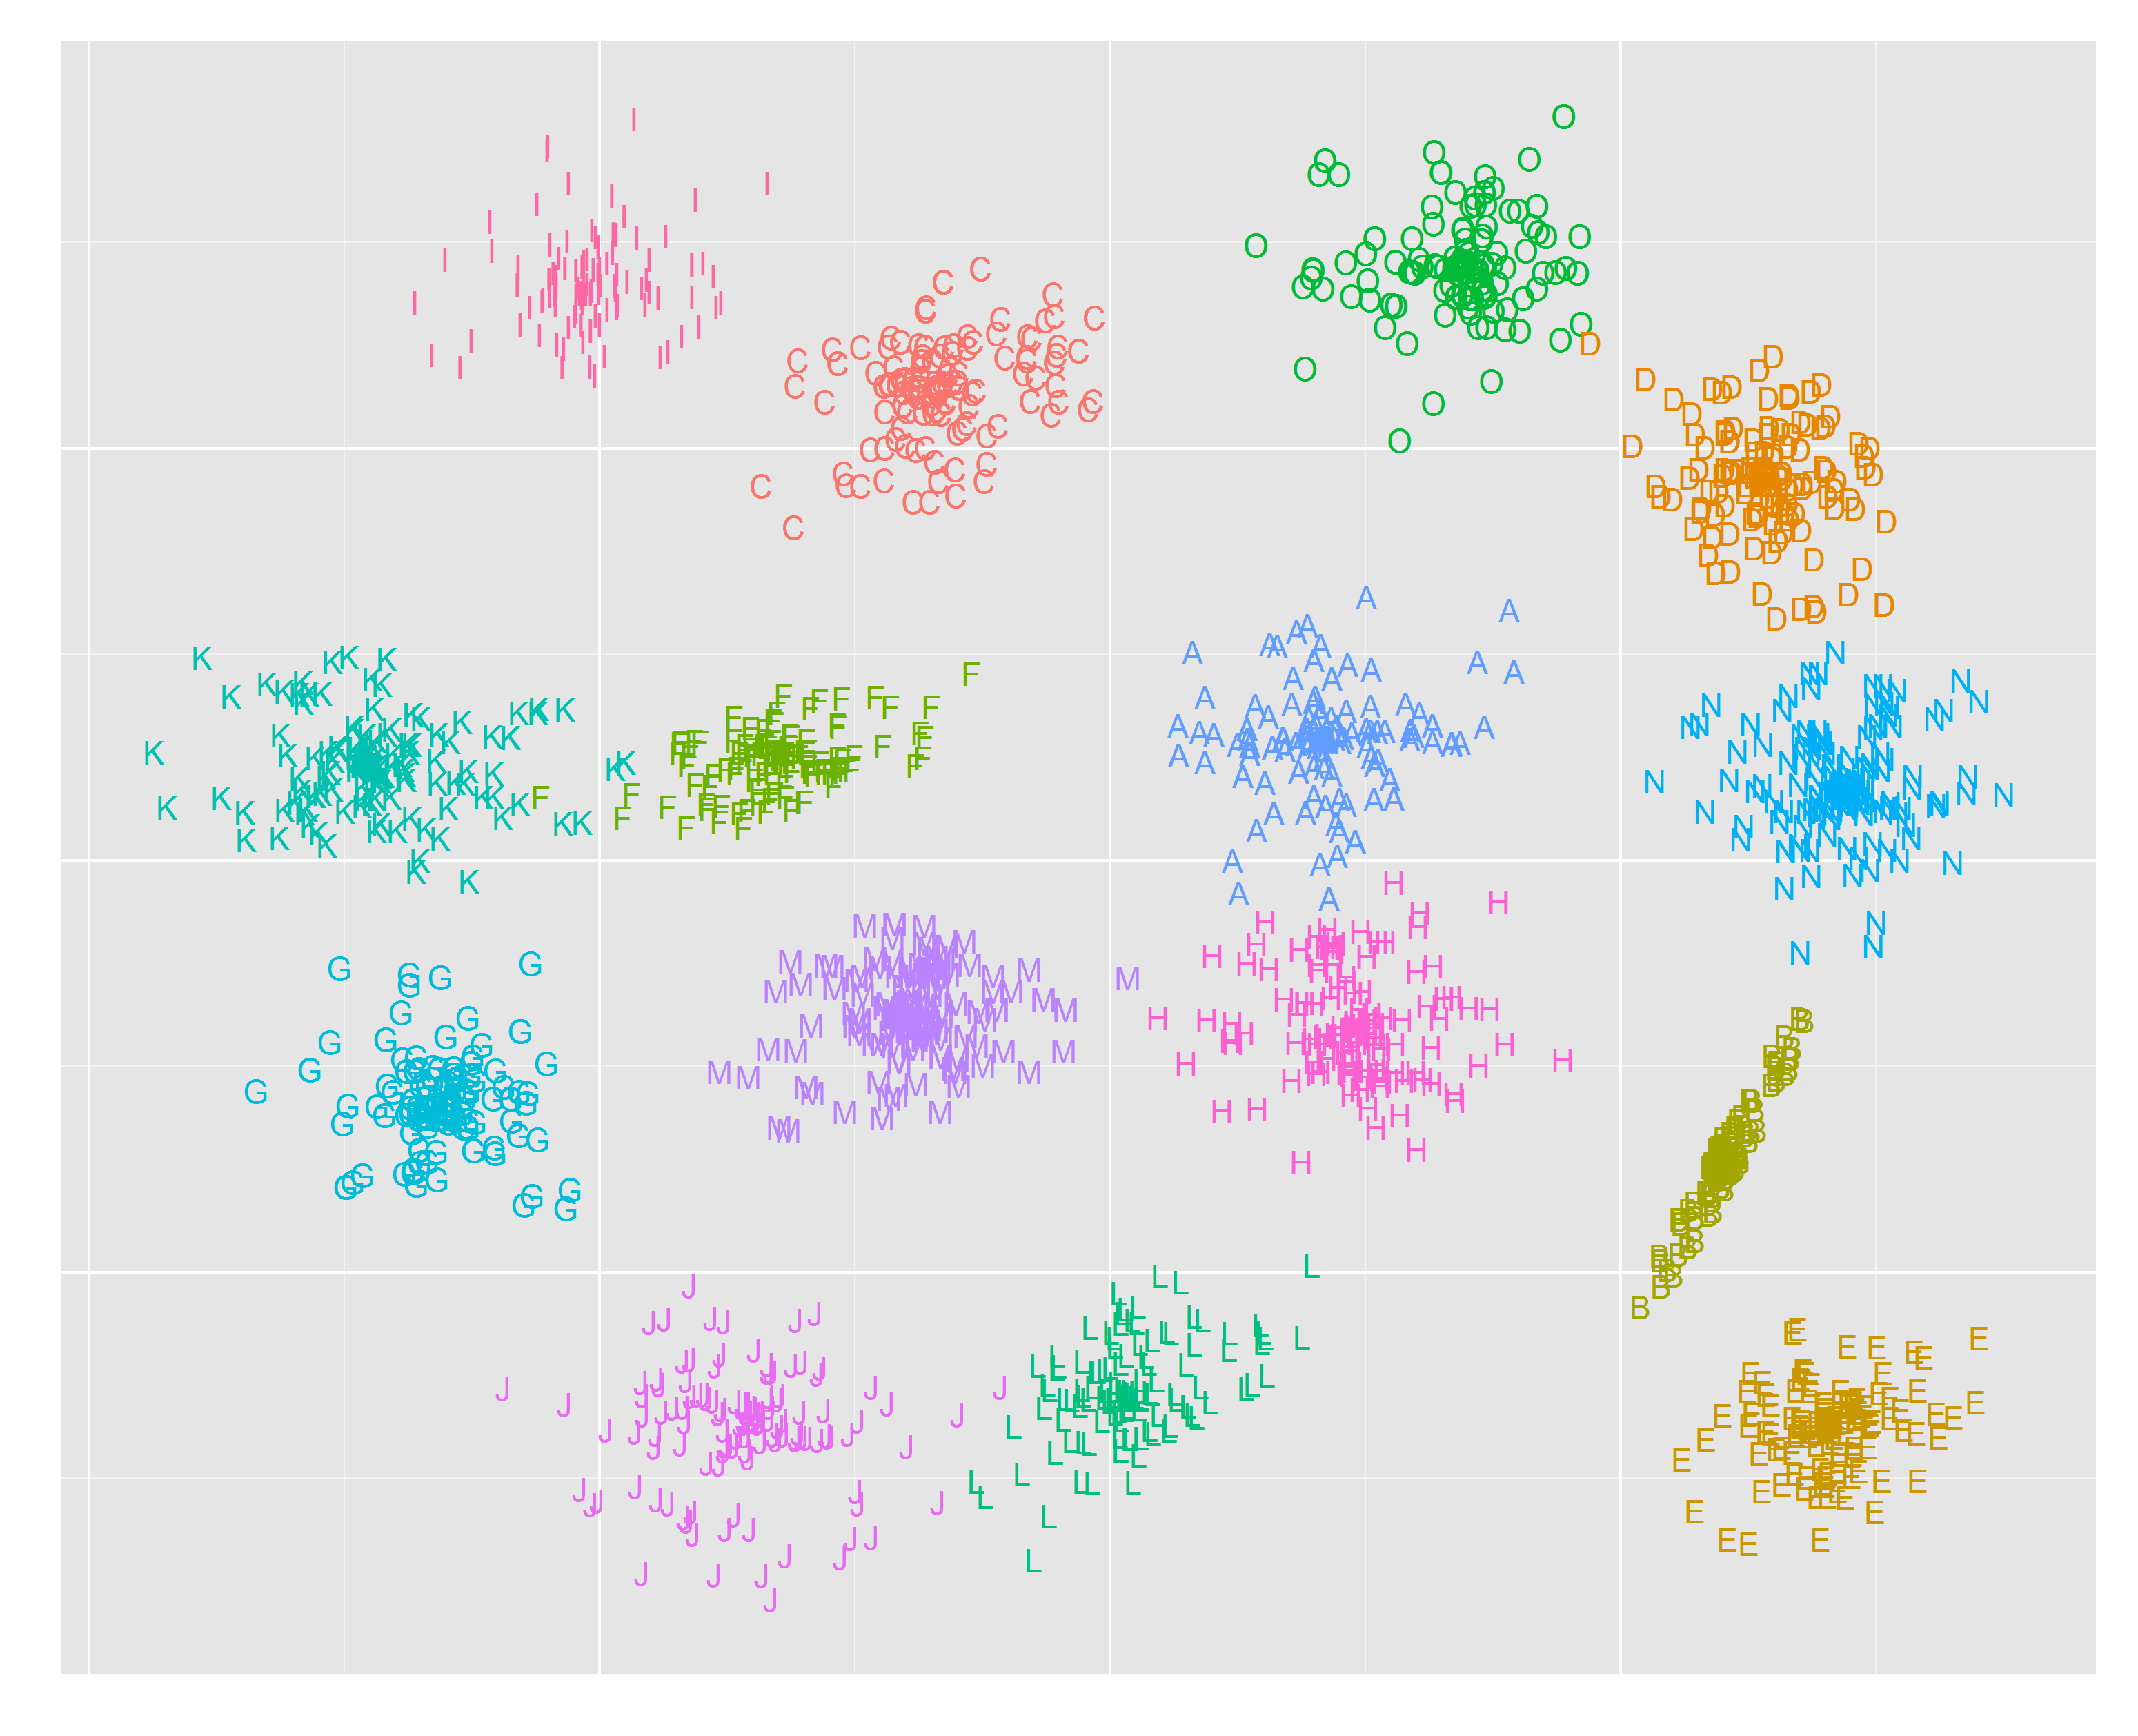
\includegraphics[width=.9\linewidth]{s_set/s_set_1_truth.png}
  \caption{S1.}
 % \label{fig:sfig1}
\end{subfigure}%
\begin{subfigure}{.4\textwidth}
  \centering
  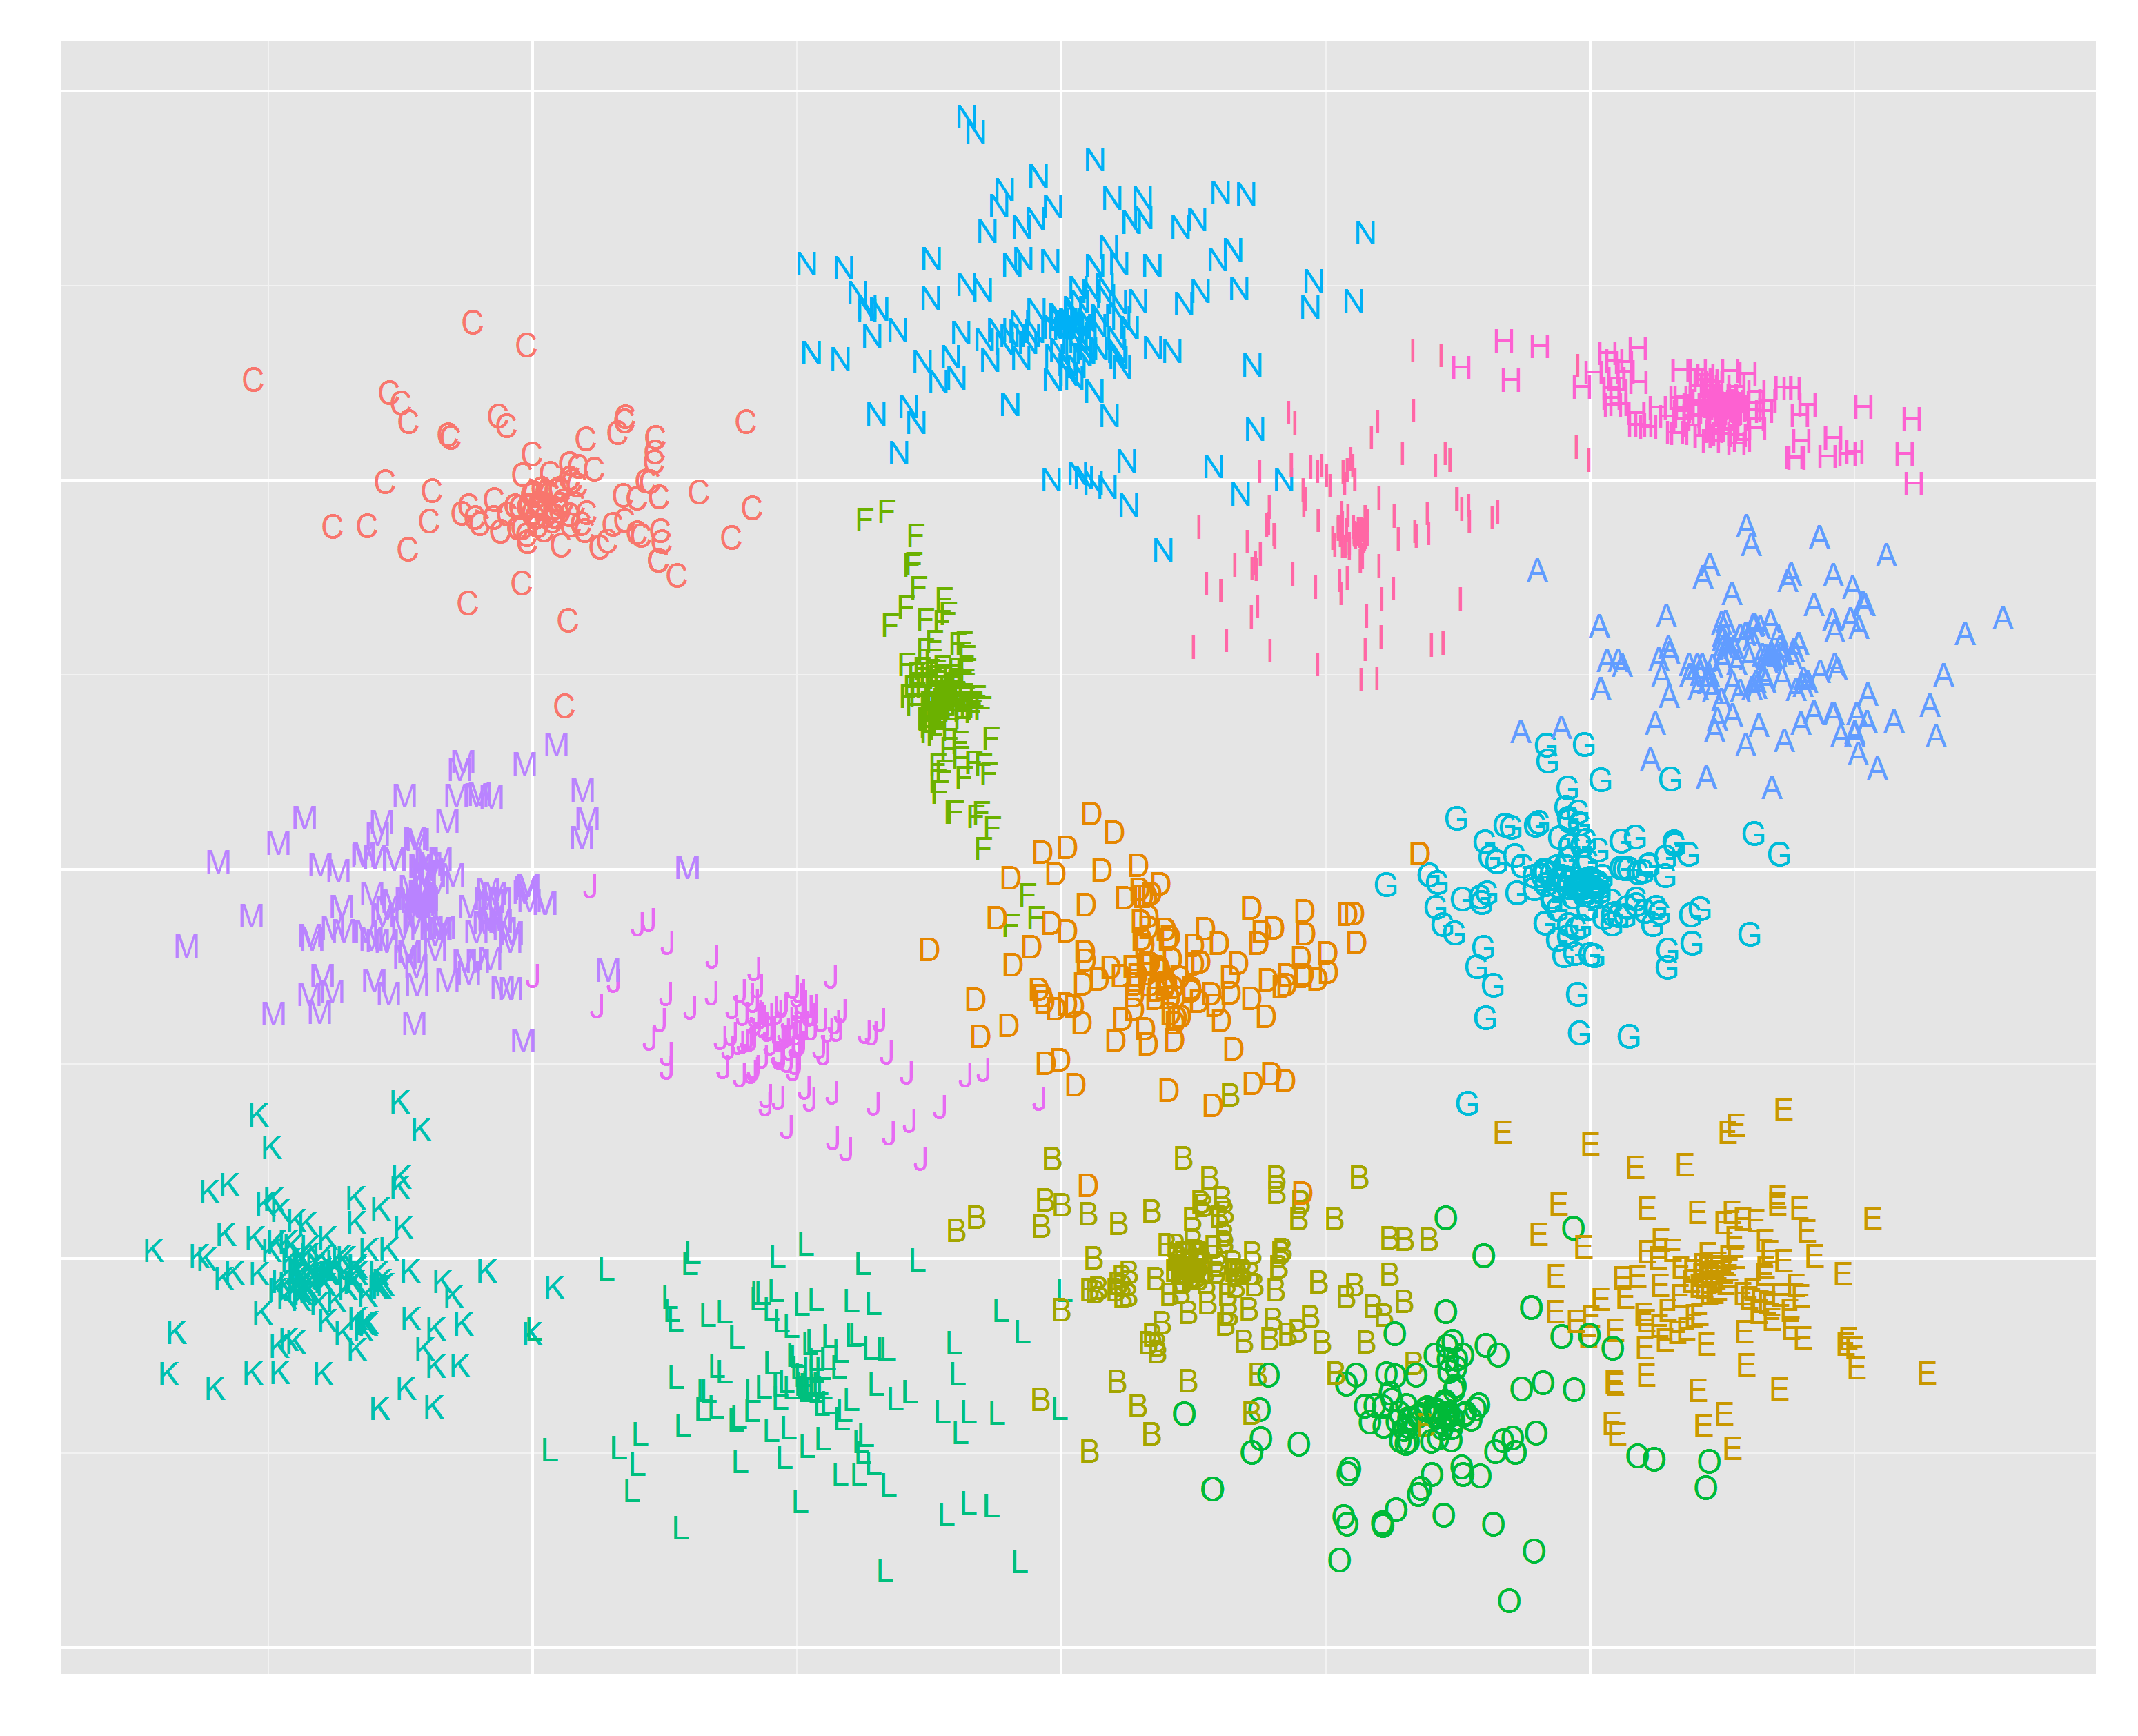
\includegraphics[width=.9\linewidth]{s_set/s_set_2_truth.png}
  \caption{S2.}
%  \label{fig:sfig2}
\end{subfigure}

\begin{subfigure}{.4\textwidth}
  \centering
  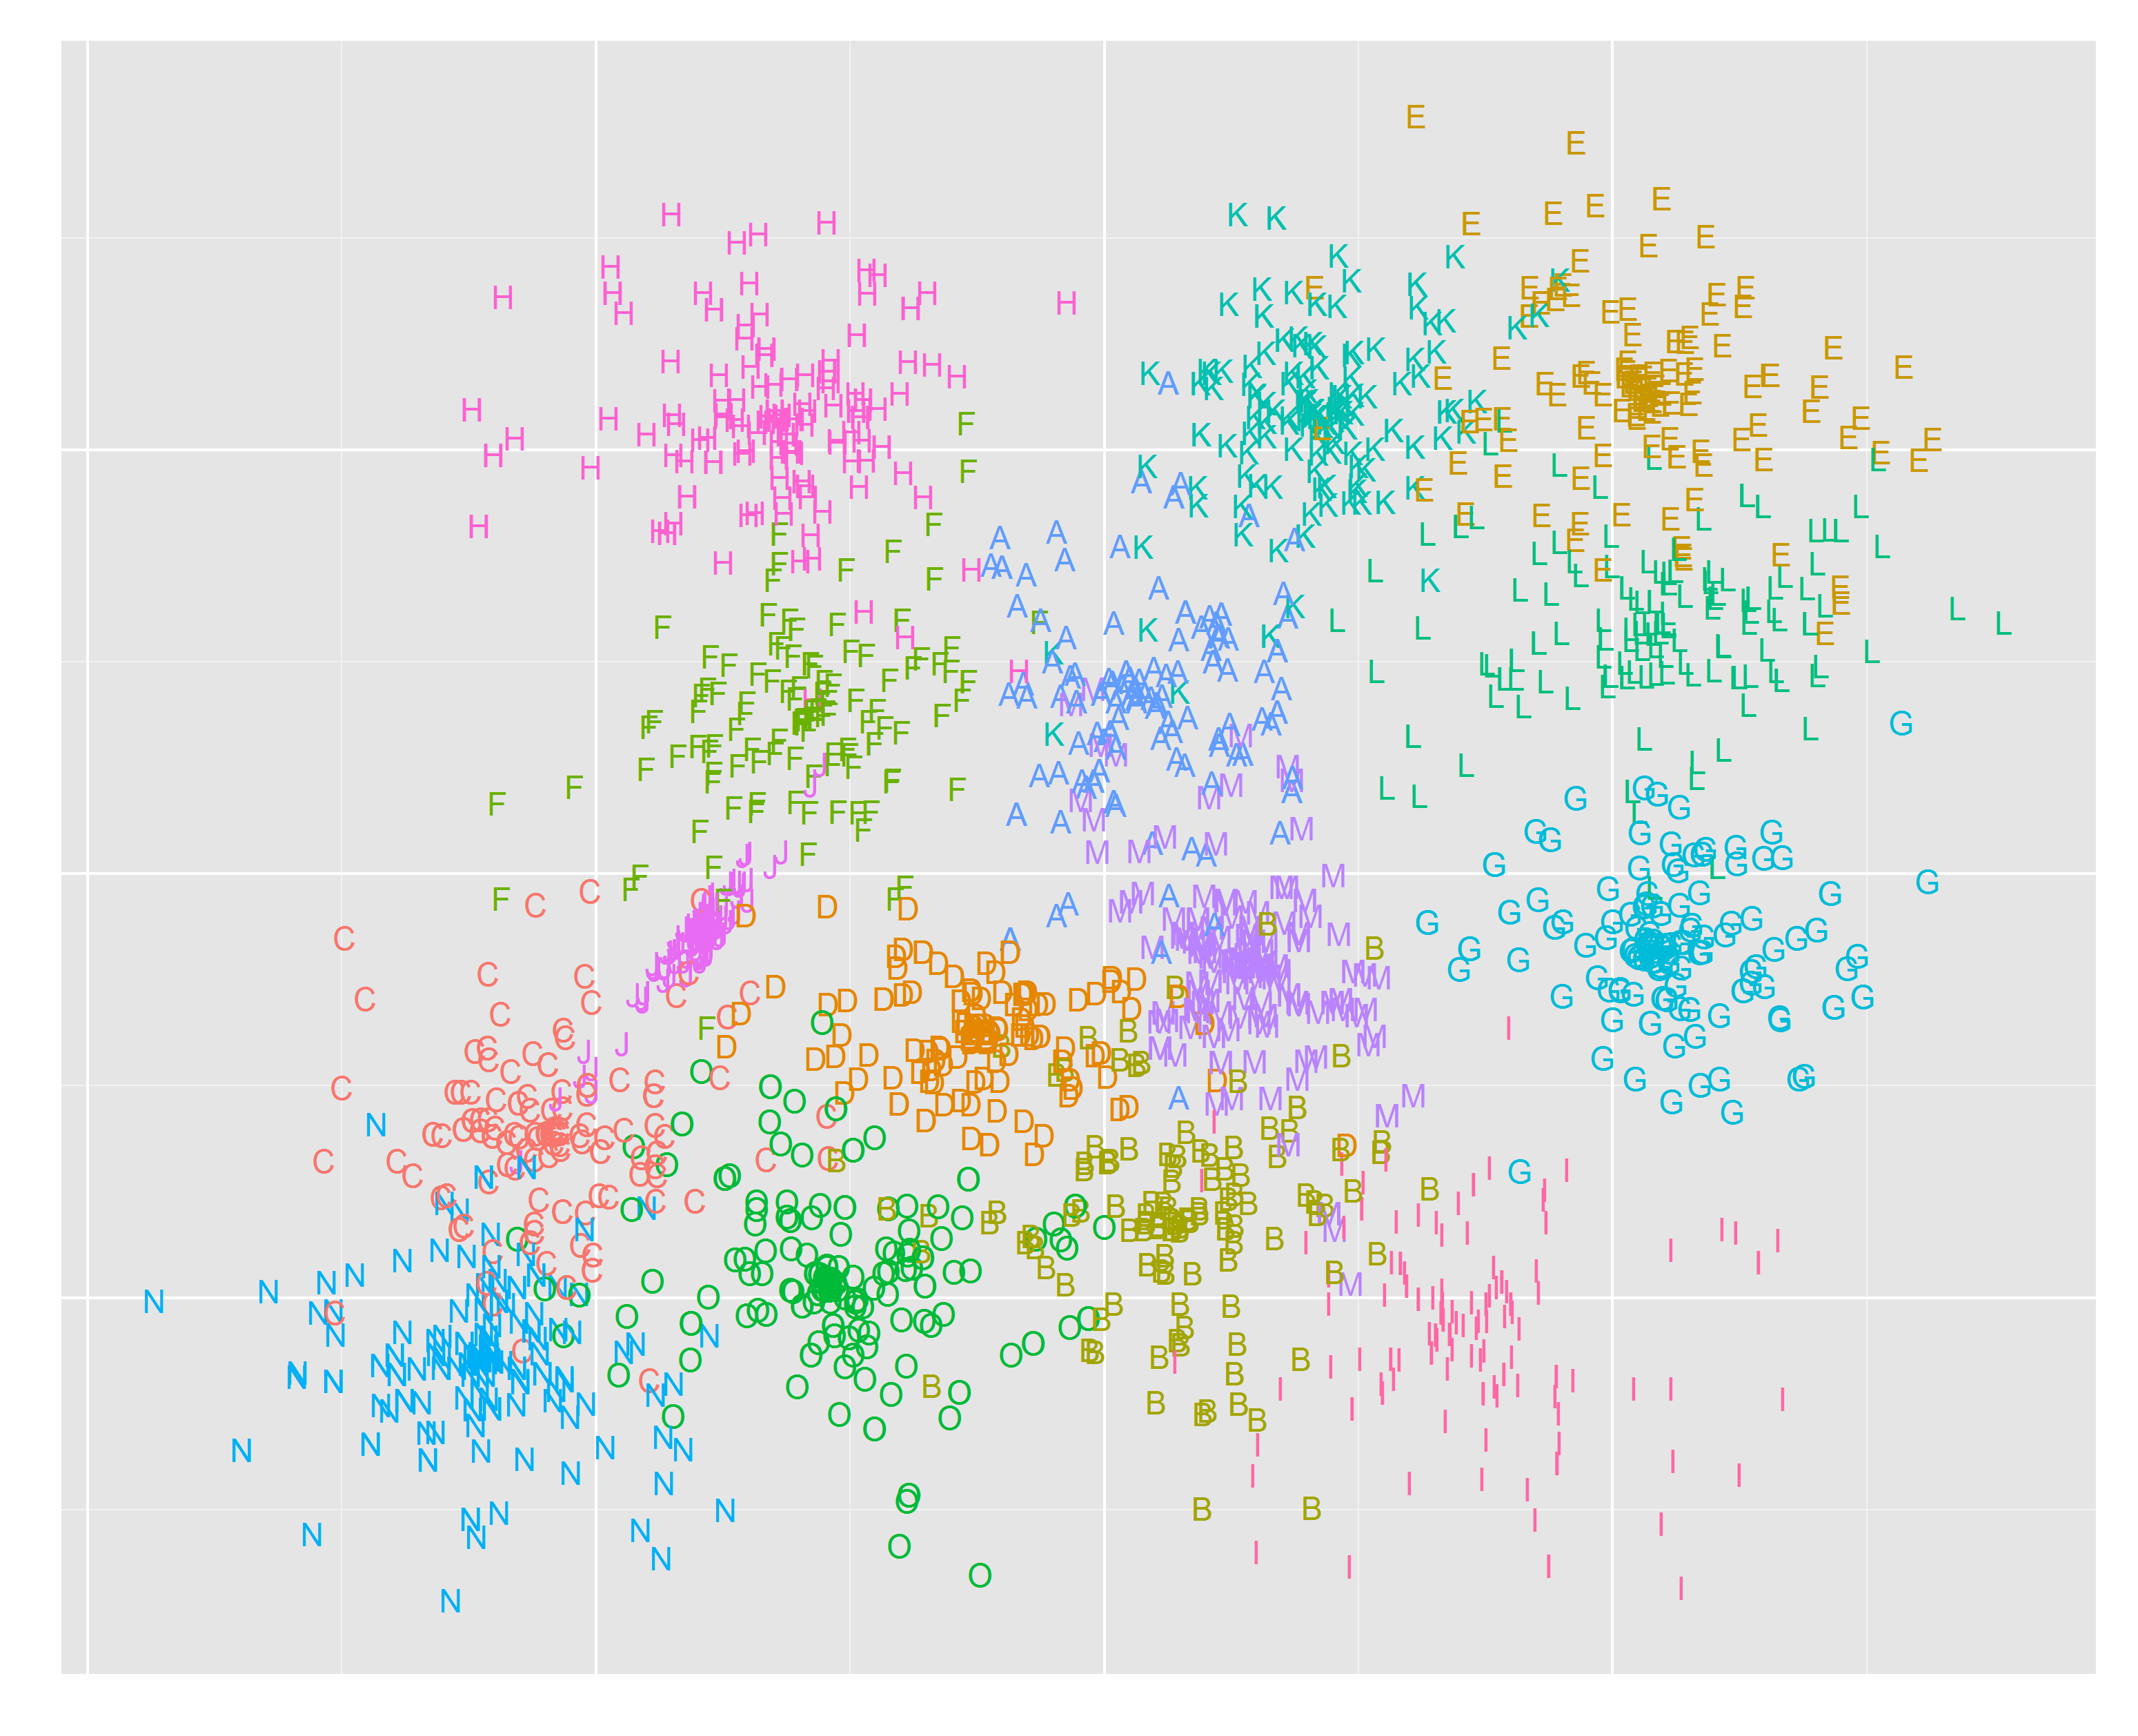
\includegraphics[width=.9\linewidth]{s_set/s_set_3_truth.png}
  \caption{S3.}
 % \label{fig:sfig1}
\end{subfigure}%
\begin{subfigure}{.4\textwidth}
  \centering
  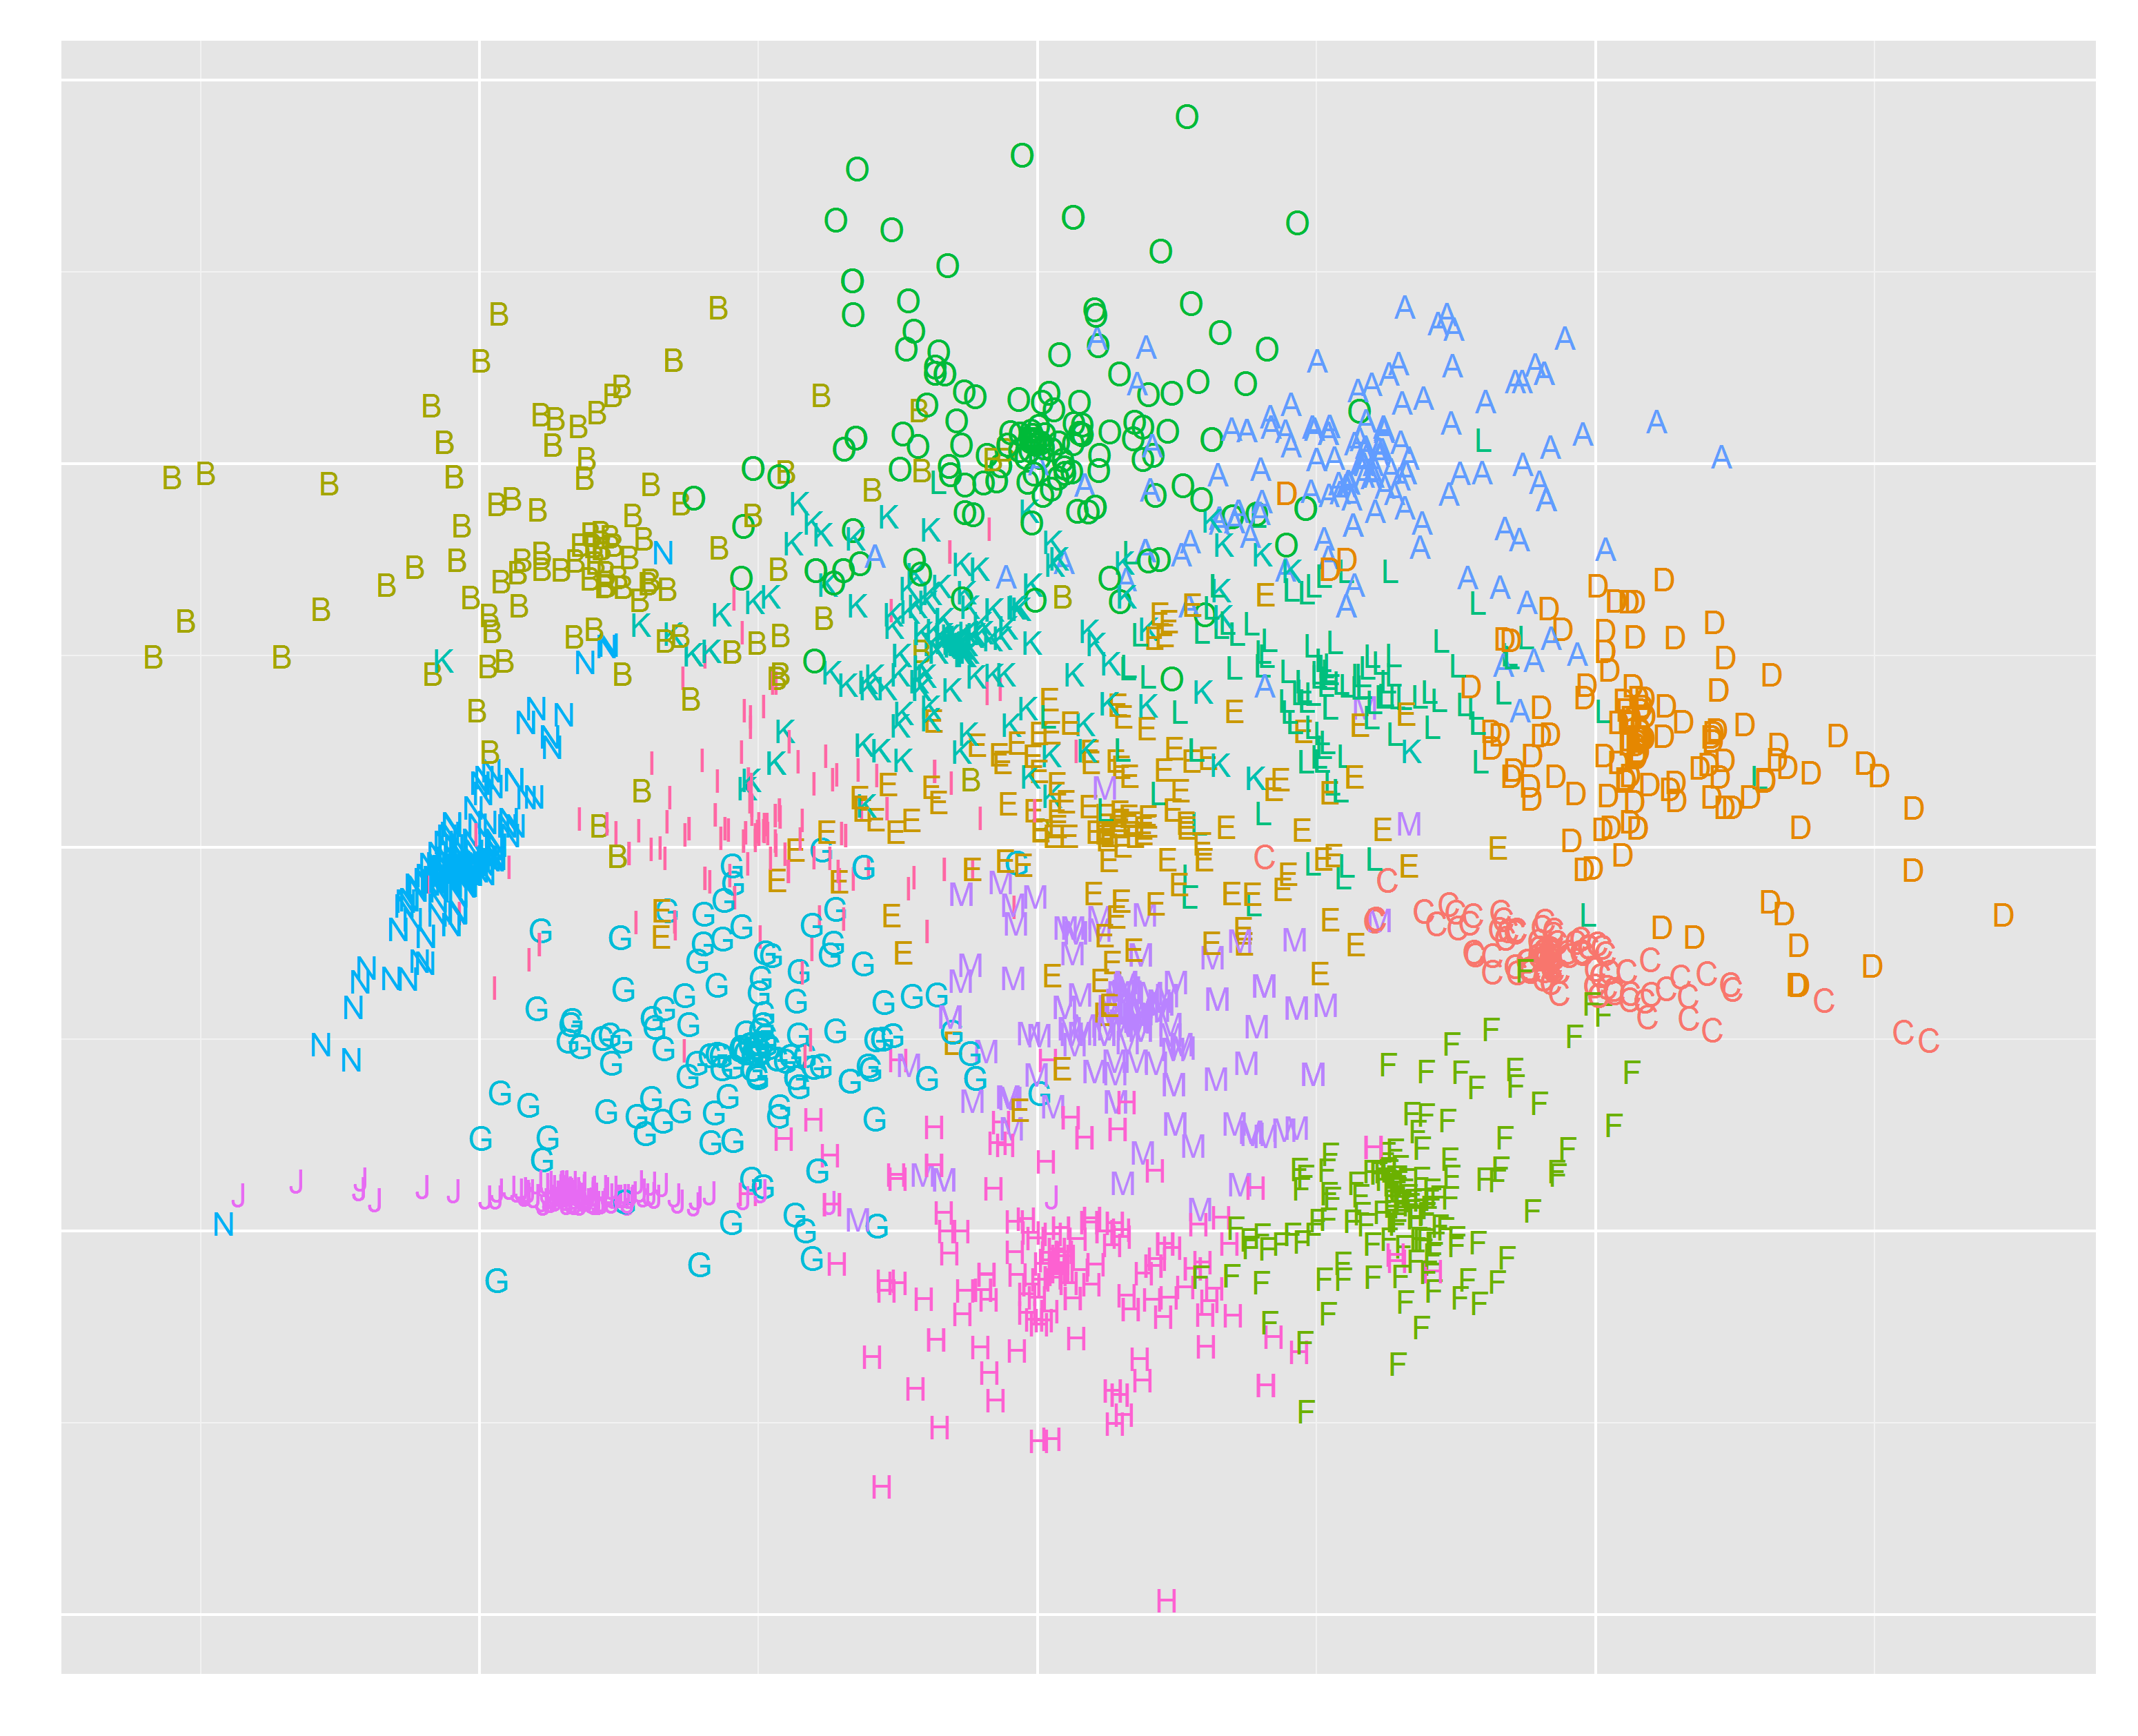
\includegraphics[width=.9\linewidth]{s_set/s_set_4_truth.png}
  \caption{S4.}
%  \label{fig:sfig2}
\end{subfigure}
\caption{The S sets \citep{Franti2006}, two-dimensional data sets with varying degrees of overlap. The true clusters labels are shown. }
\label{fig:s_set_truth}
\end{figure}



 Each set consists of synthetic two-dimensional data with $n$=5000 data points and $k$=15 Gaussian clusters with different degrees of cluster overlapping. Data set S1 should be the easiest to cluster as all 15 clusters are well fairly separated. The sets become increasingly more challenging and S4 can be difficult even for humans to separate correctly.  We treated each of these data sets as a data stream and used spectral CluStream and windowed spectral clustering to assign data points to clusters. Performance is evaluated in batch every $10^{th}$ time point. The results are shown in Figures \ref{fig:s_set_purity} and \ref{fig:s_set_vmeasure}. 

%%% Purity plots
\begin{figure}[H]
\begin{subfigure}{.45\textwidth}
  \centering
  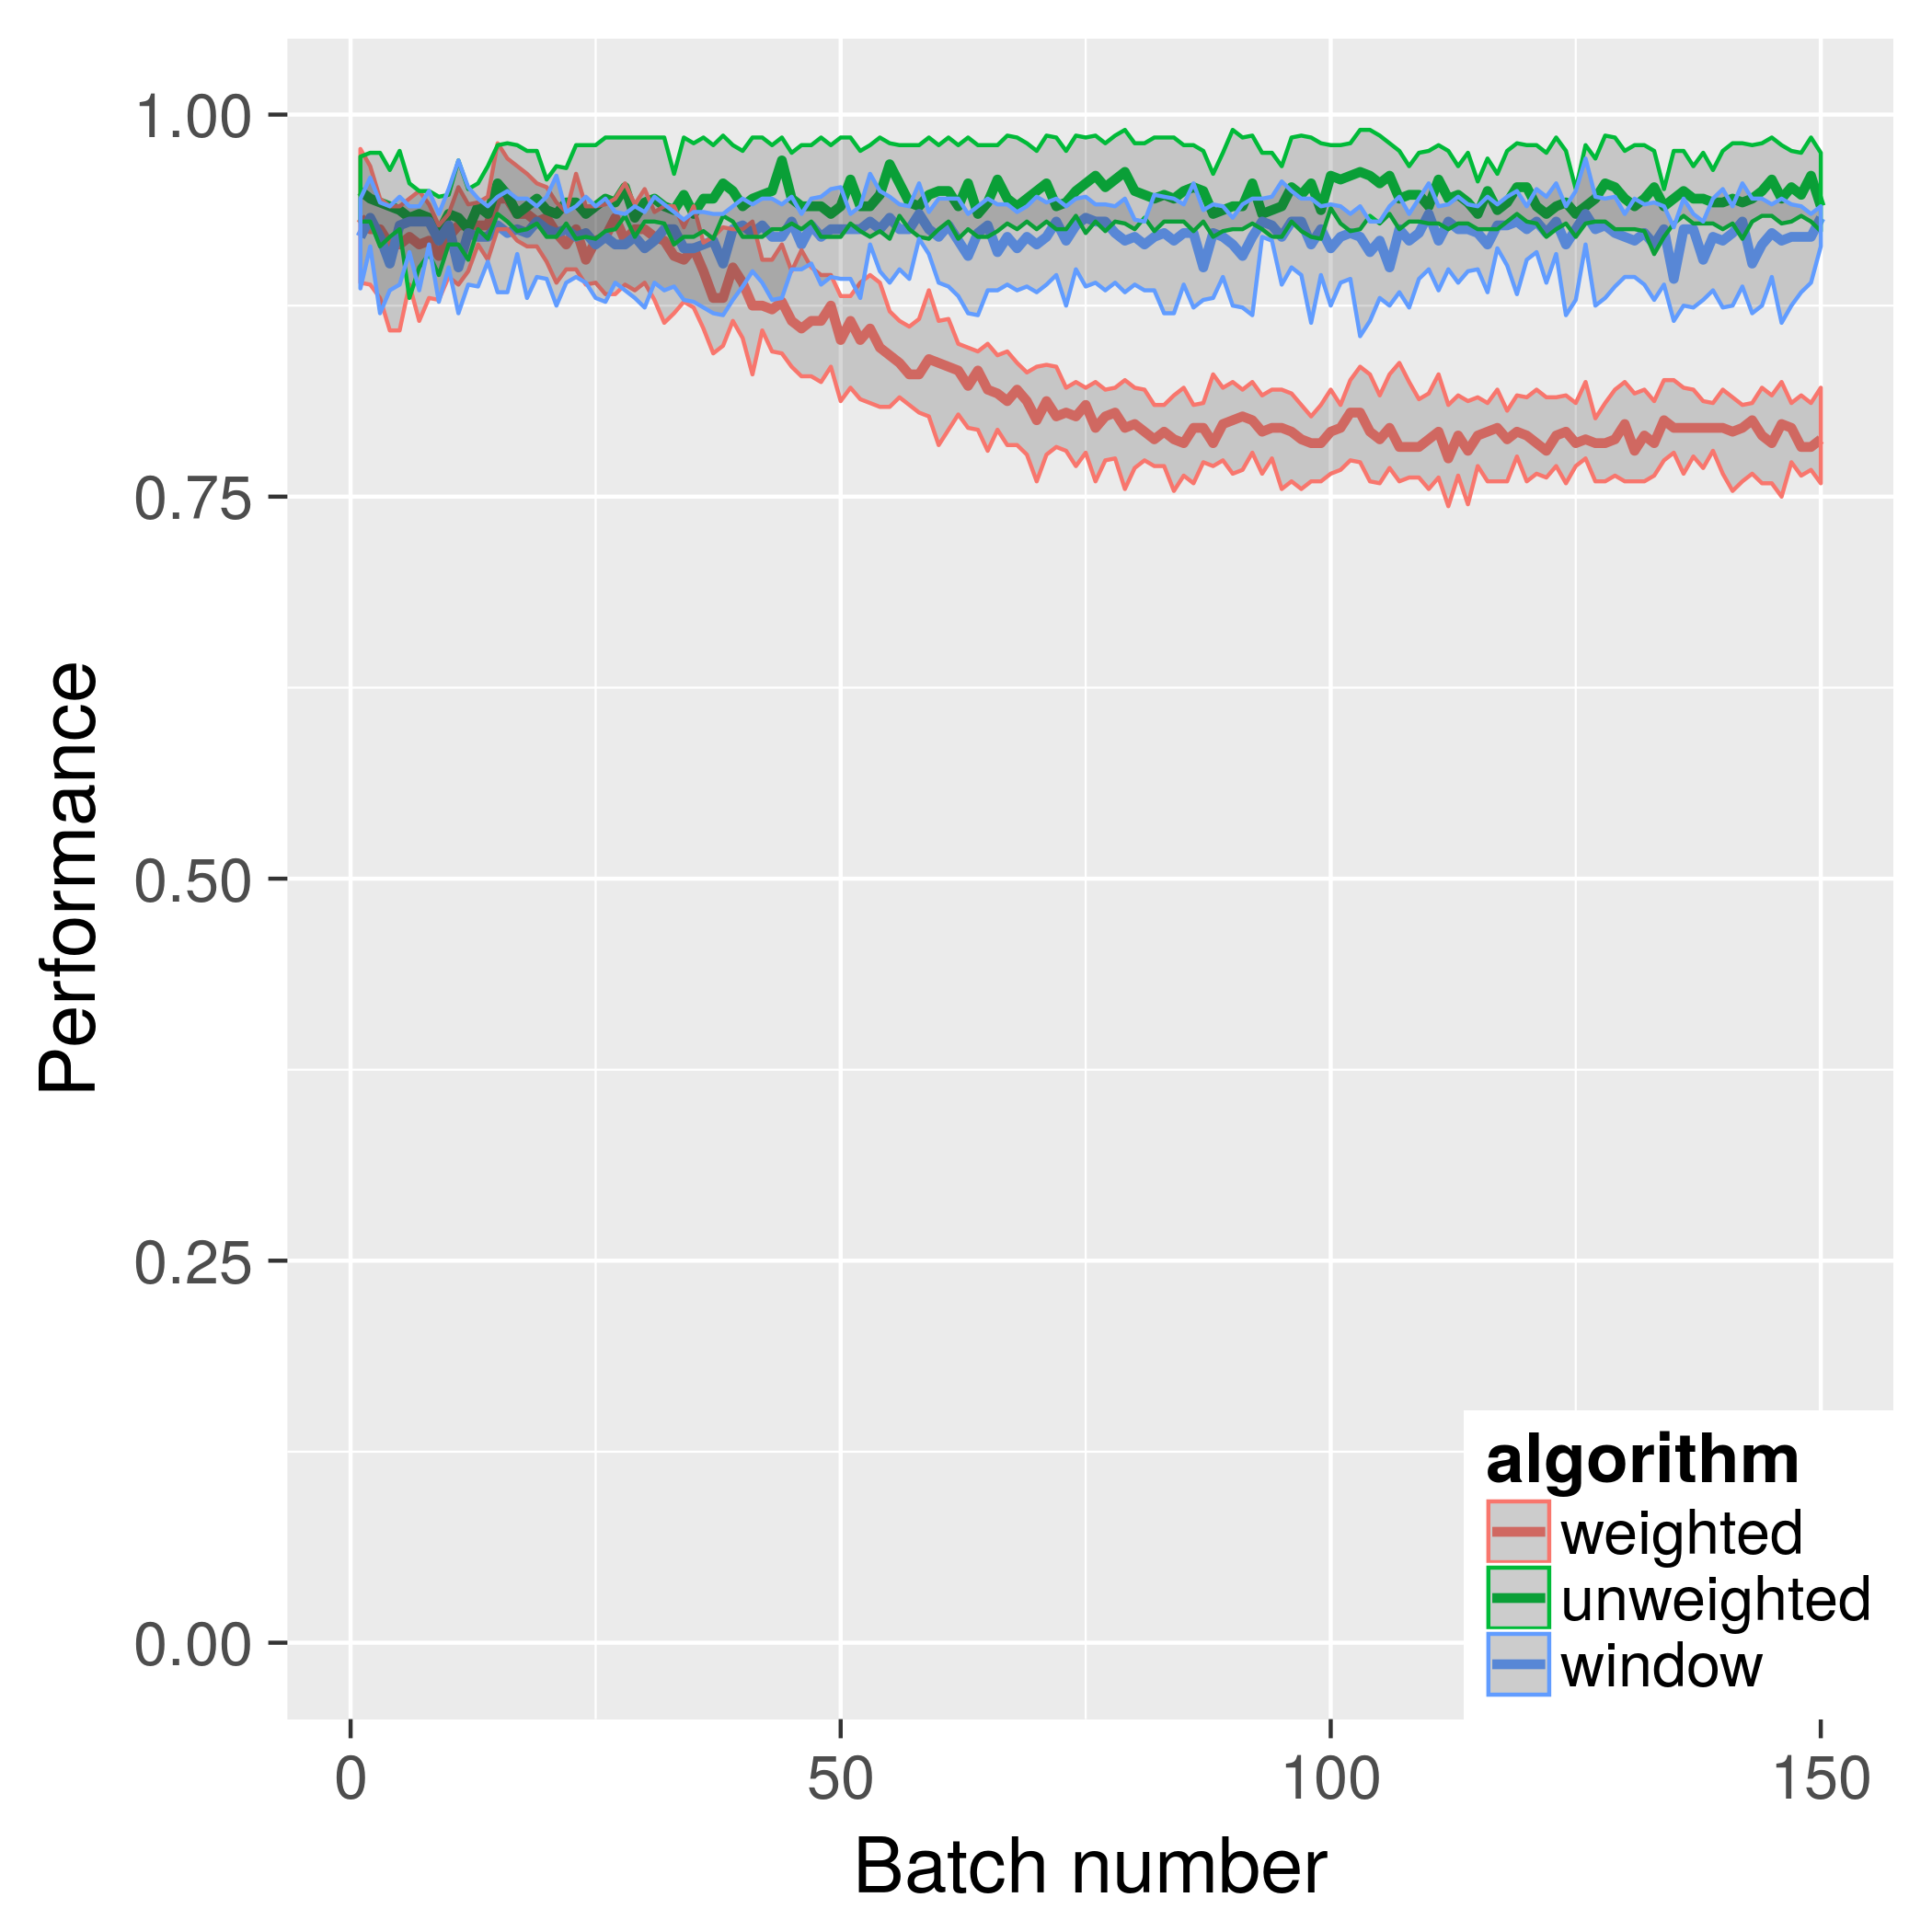
\includegraphics[width=.9\linewidth]{s_set/s_set_1_with_weighted_ci_one_size_purity.png}
  \caption{S1.}
\end{subfigure}%
\begin{subfigure}{.45\textwidth}
  \centering
  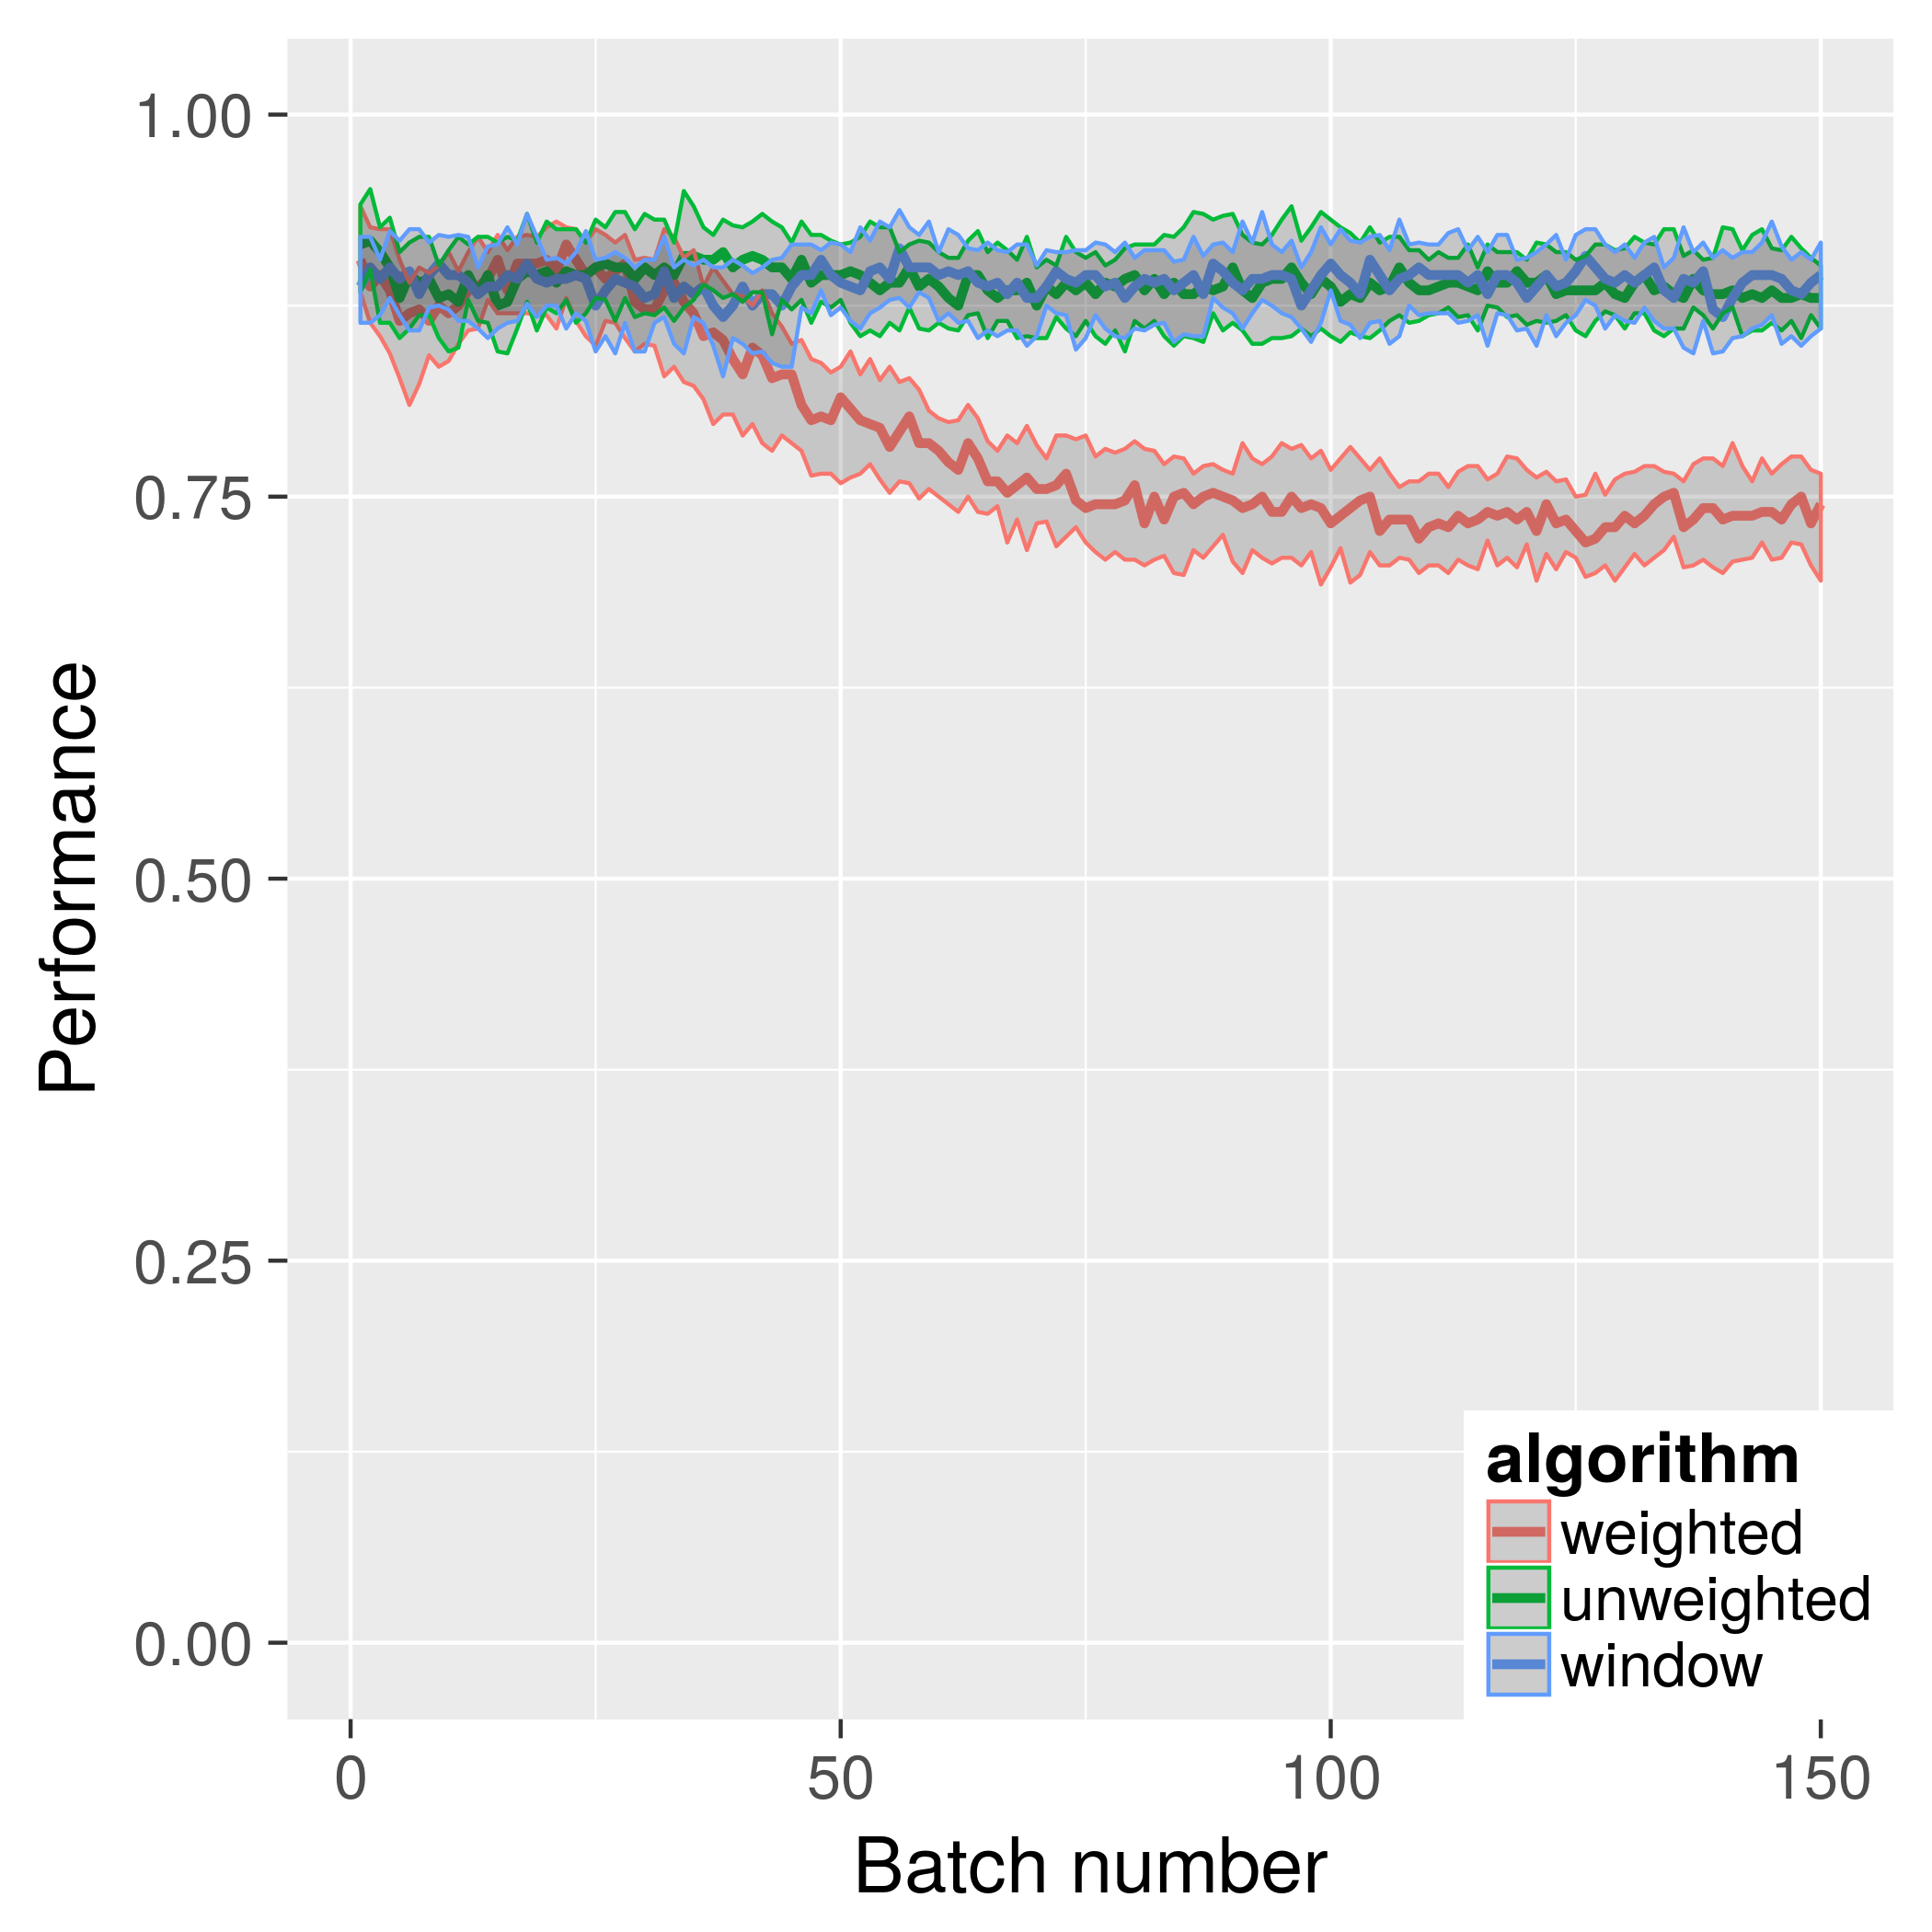
\includegraphics[width=.9\linewidth]{s_set/s_set_2_with_weighted_ci_one_size_purity.png}
  \caption{S2.}
\end{subfigure}
\begin{subfigure}{.45\textwidth}
  \centering
  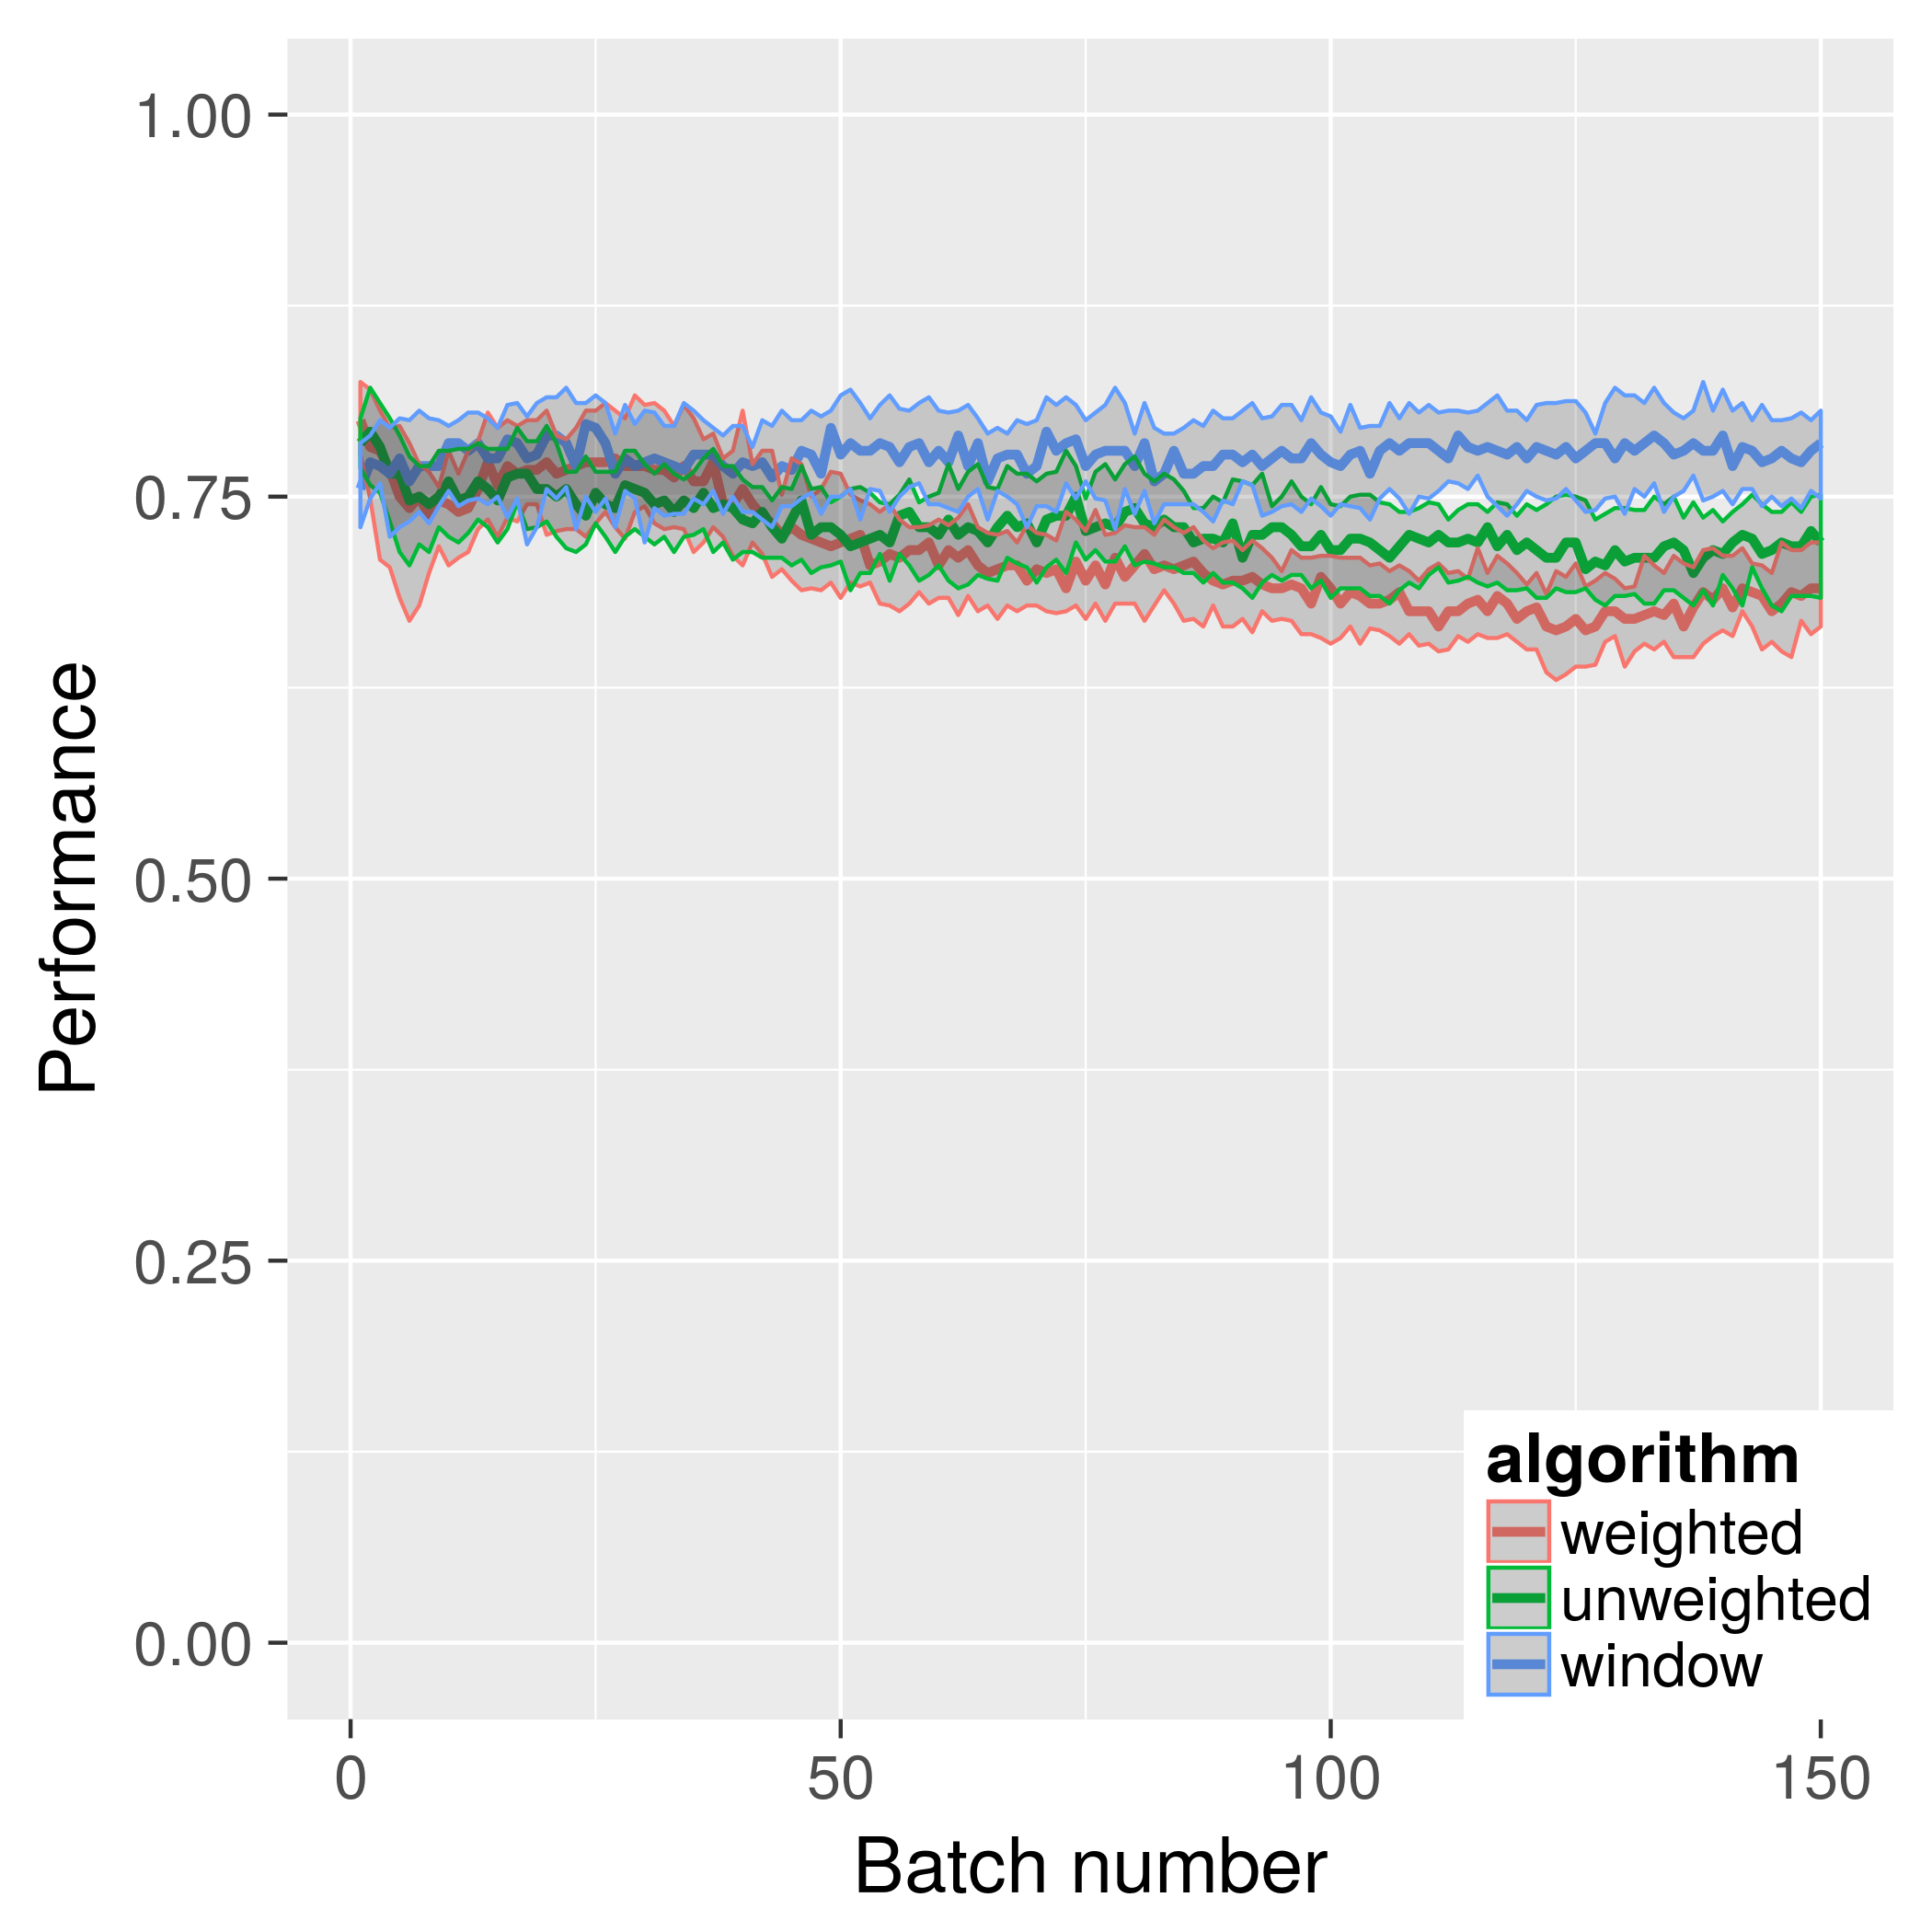
\includegraphics[width=.9\linewidth]{s_set/s_set_3_with_weighted_ci_one_size_purity.png}
  \caption{S3.}
\end{subfigure}%
\begin{subfigure}{.45\textwidth}
  \centering
  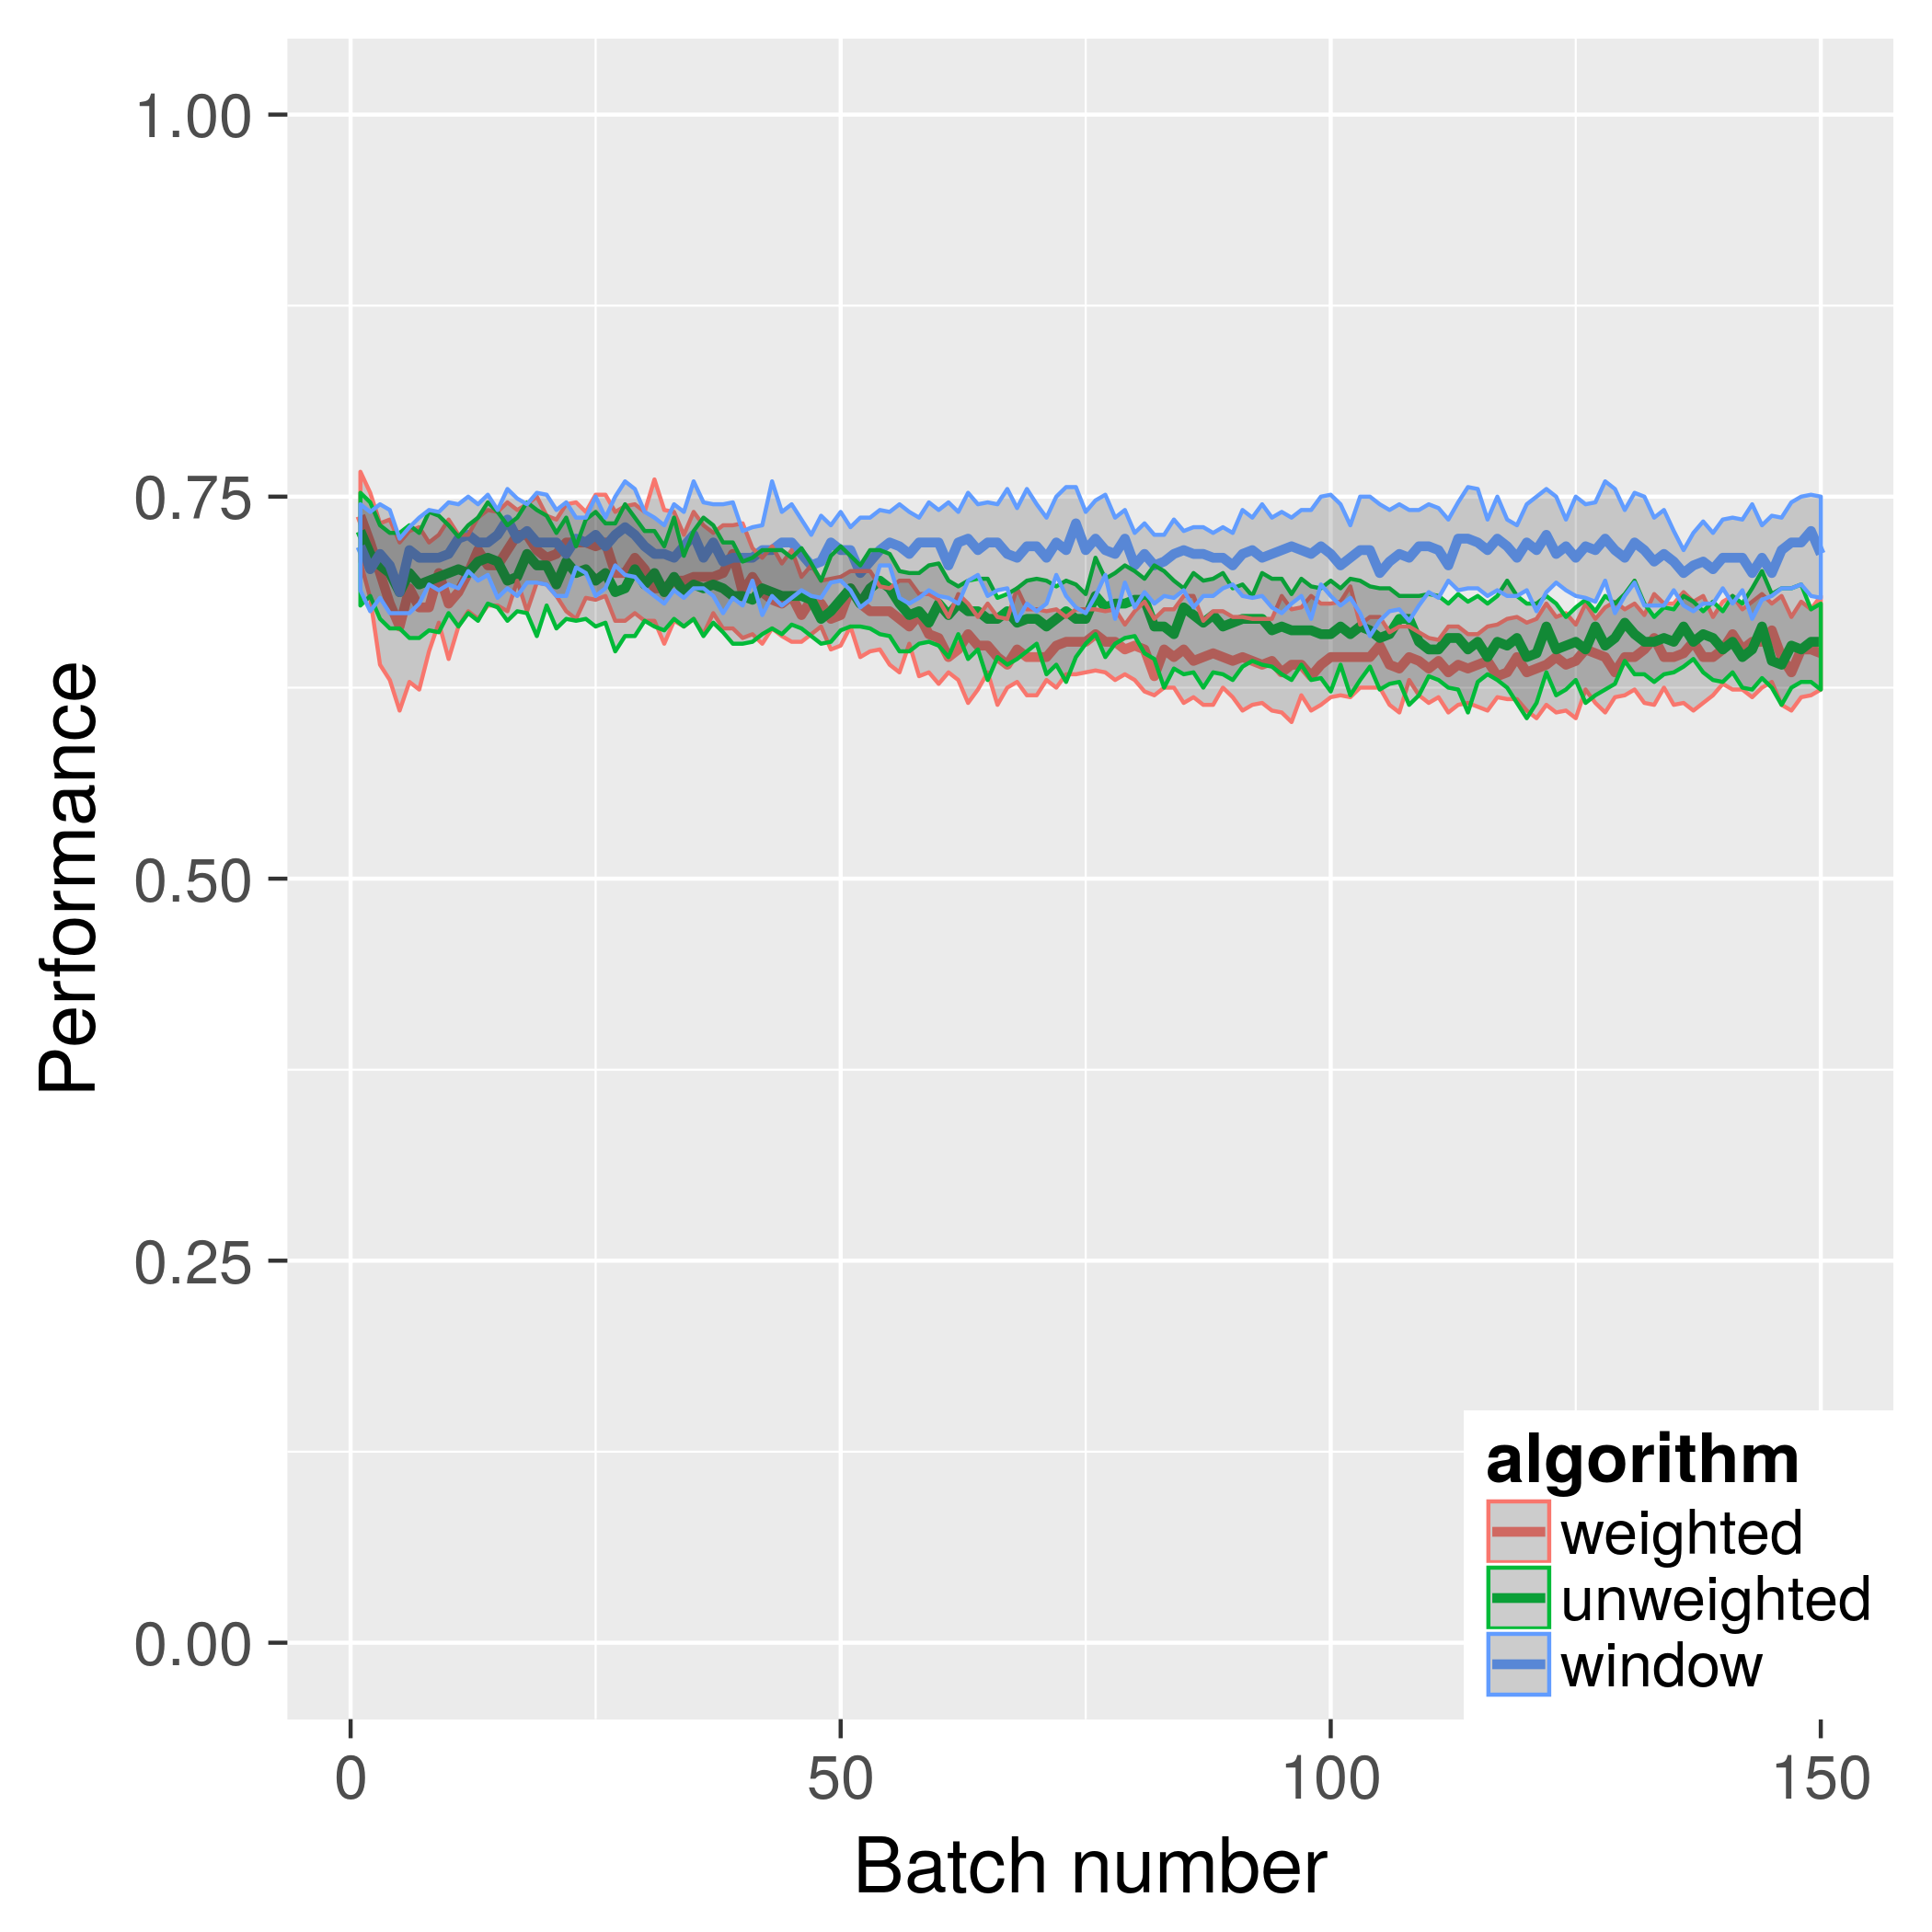
\includegraphics[width=.9\linewidth]{s_set/s_set_4_with_weighted_ci_one_size_purity.png}
  \caption{S4.}
\end{subfigure}
\caption{Purity for the S data sets.}
\label{fig:s_set_purity}
\end{figure}

Figure \ref{fig:s_set_purity} plots the performance in terms of purity on the y-axis and the batch number is given on the x-axis. The average performance for each algorithm over the multiple runs is given by the thick solid lines and the shaded area depicts the inter-quartile range.  Figure \ref{fig:s_set_vmeasure} shows the performance in terms of V-measure.  Both figures show the algorithm performance at each batch step, meaning that we can see how performance changes as the data stream progresses. However, these data sets are stationary in distribution and therefore we would not expect to see algorithm performance vary dramatically with time. 

%%%% V-measure plots
\begin{figure}[h]
\begin{subfigure}{.45\textwidth}
  \centering
  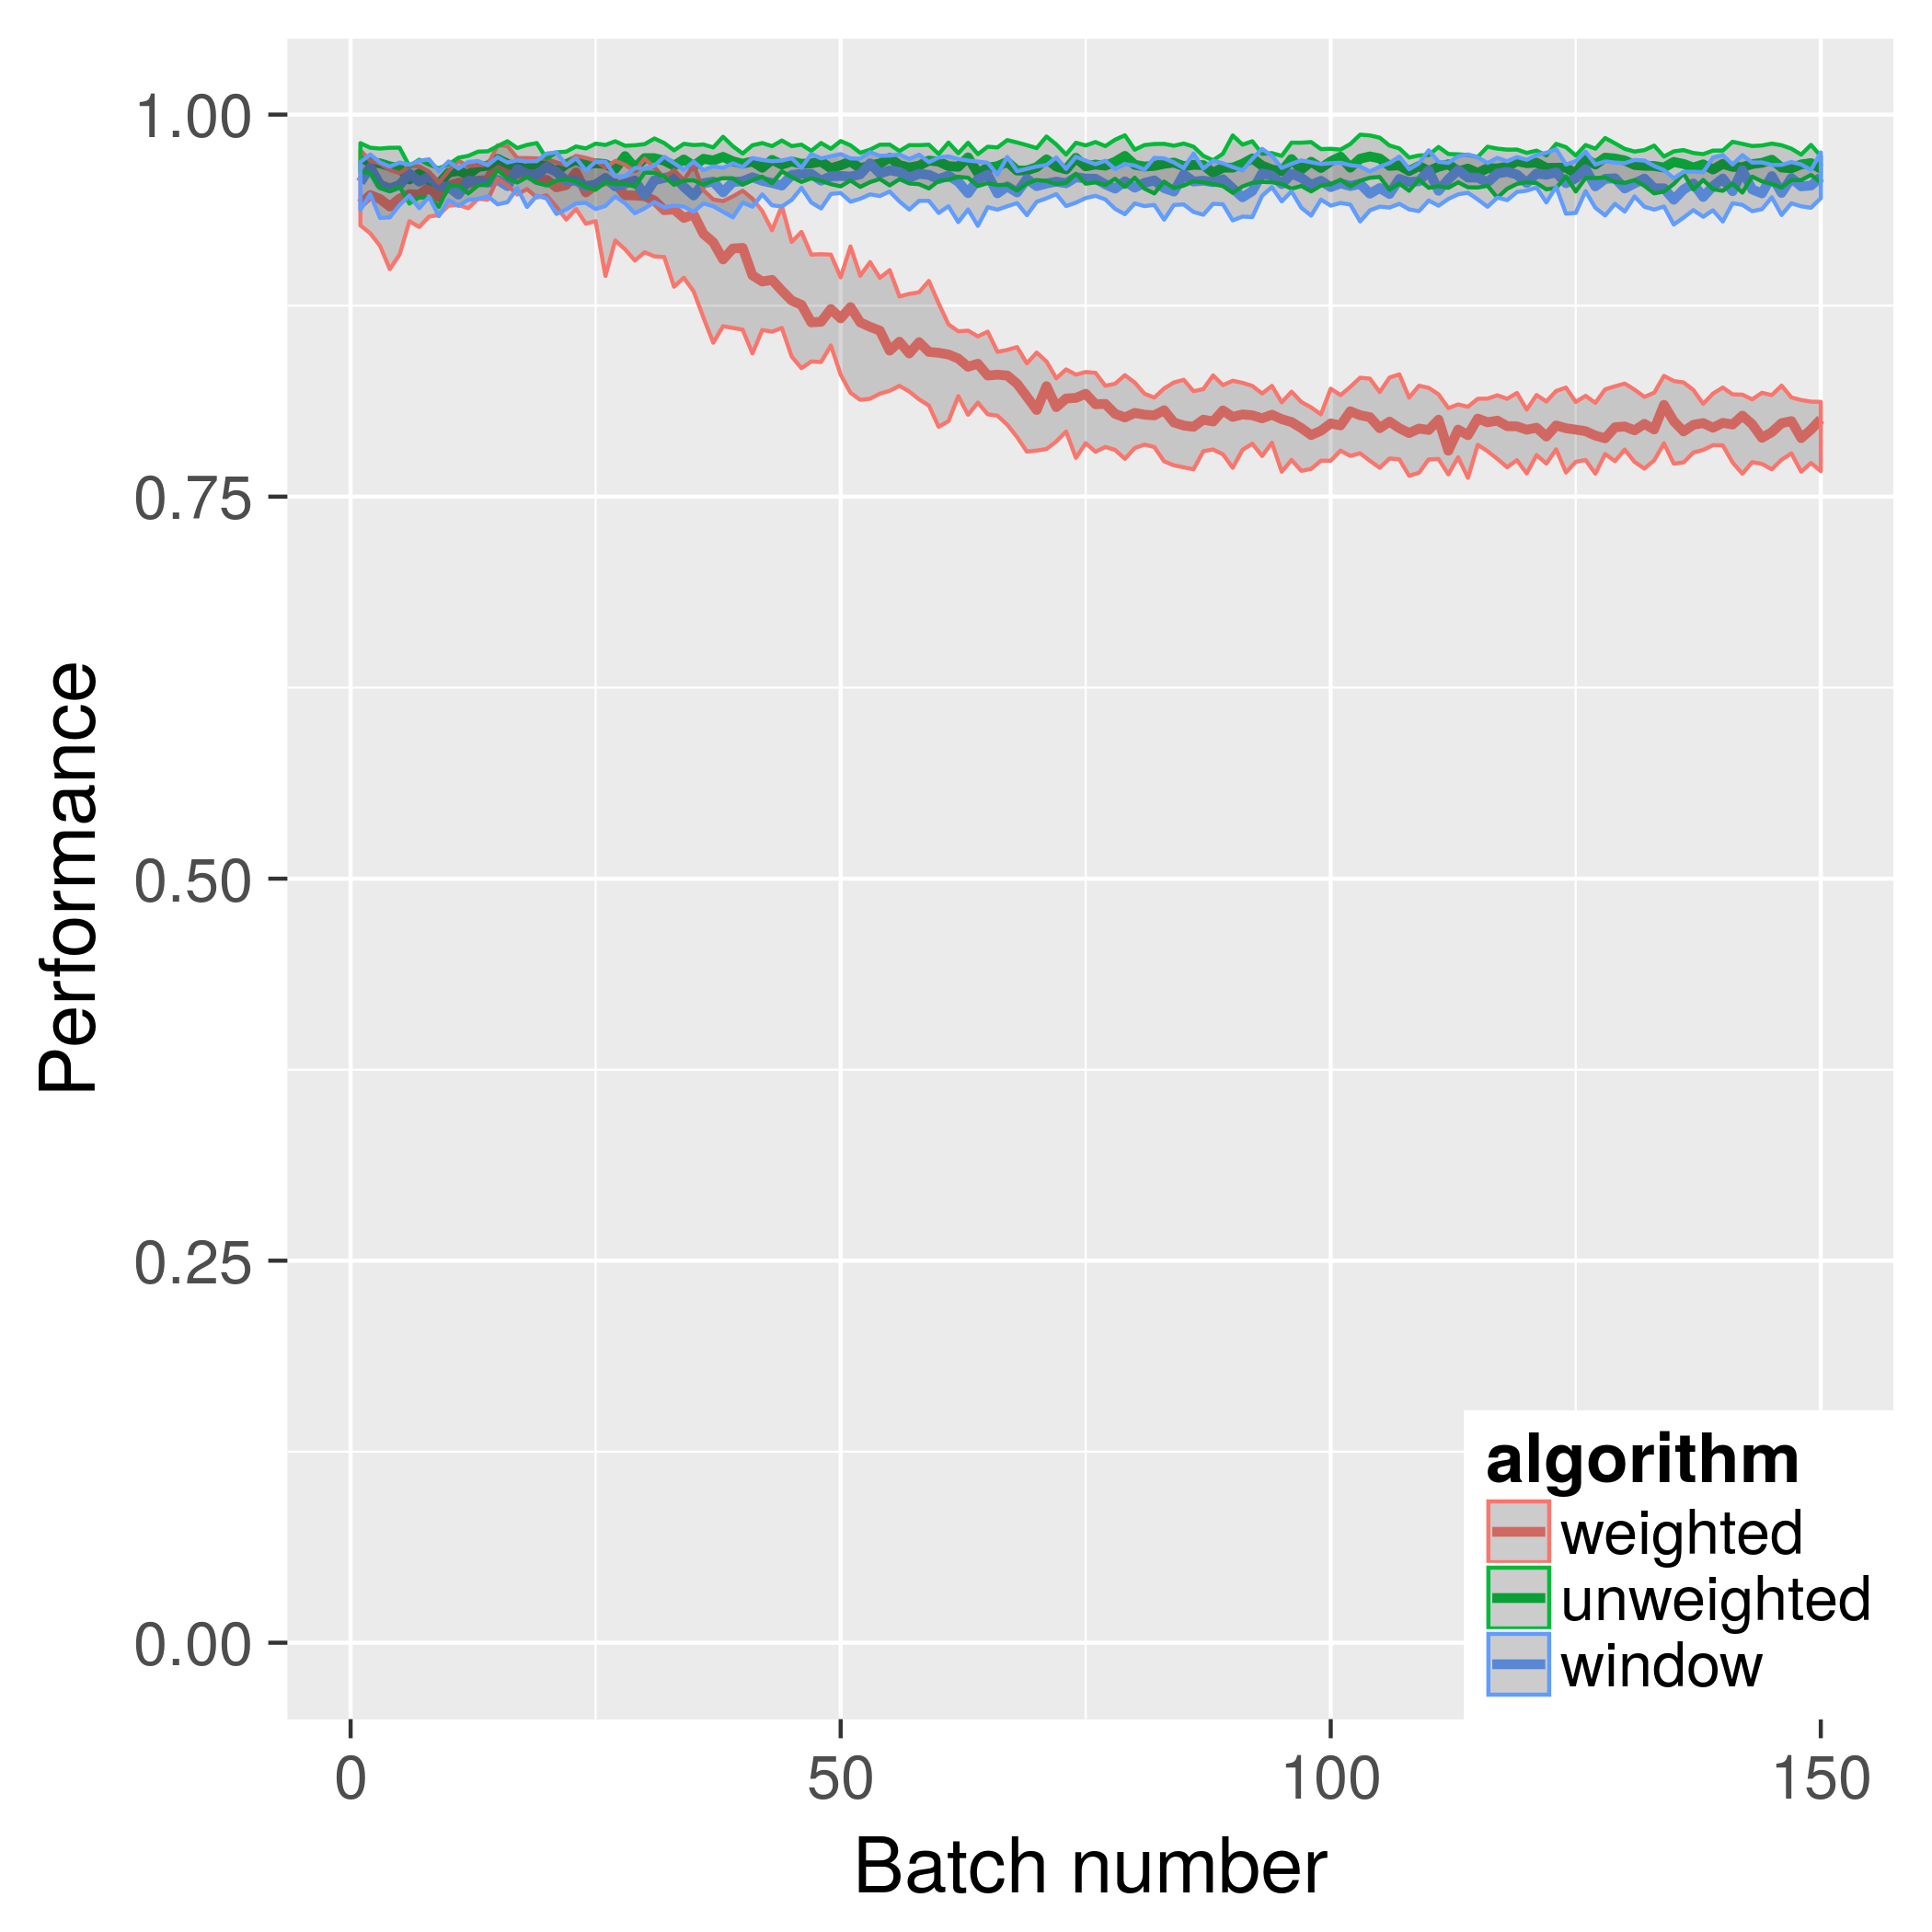
\includegraphics[width=.9\linewidth]{s_set/s_set_1_with_weighted_ci_one_size_vmeasure.png}
  \caption{S1.}
\end{subfigure}%
\begin{subfigure}{.45\textwidth}
  \centering
  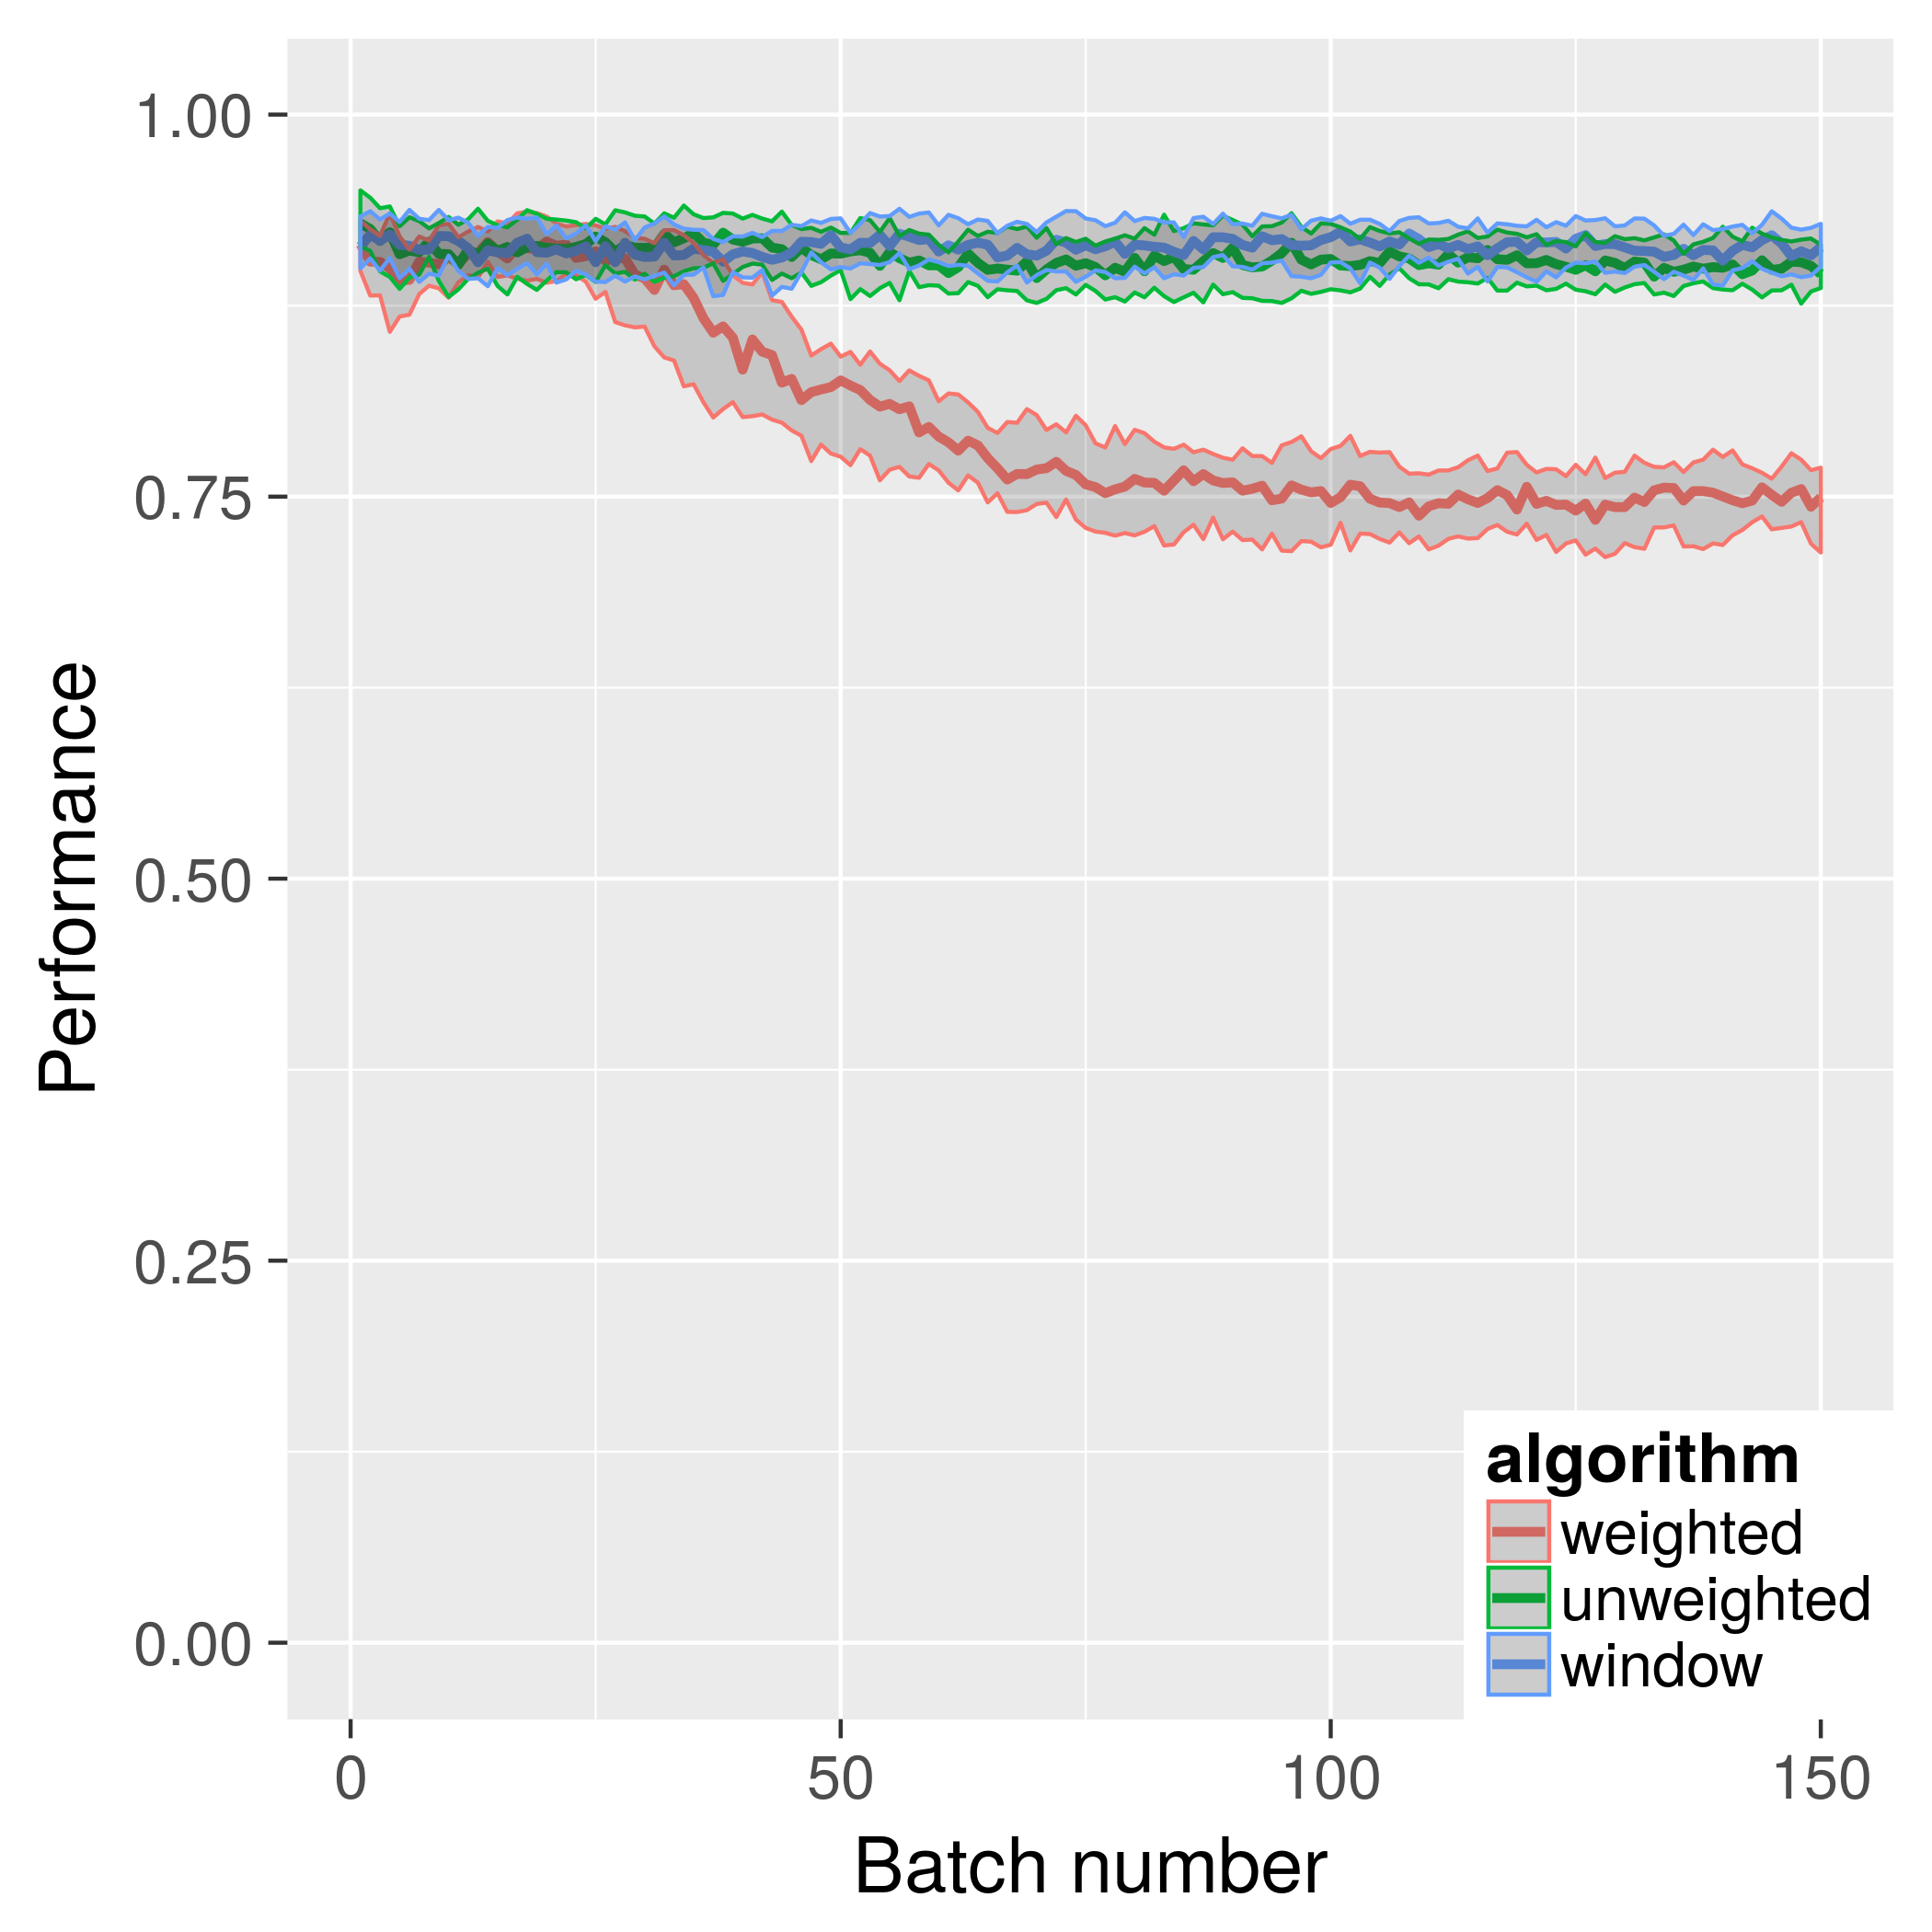
\includegraphics[width=.9\linewidth]{s_set/s_set_2_with_weighted_ci_one_size_vmeasure.png}
  \caption{S2.}
\end{subfigure}
\begin{subfigure}{.45\textwidth}
  \centering
  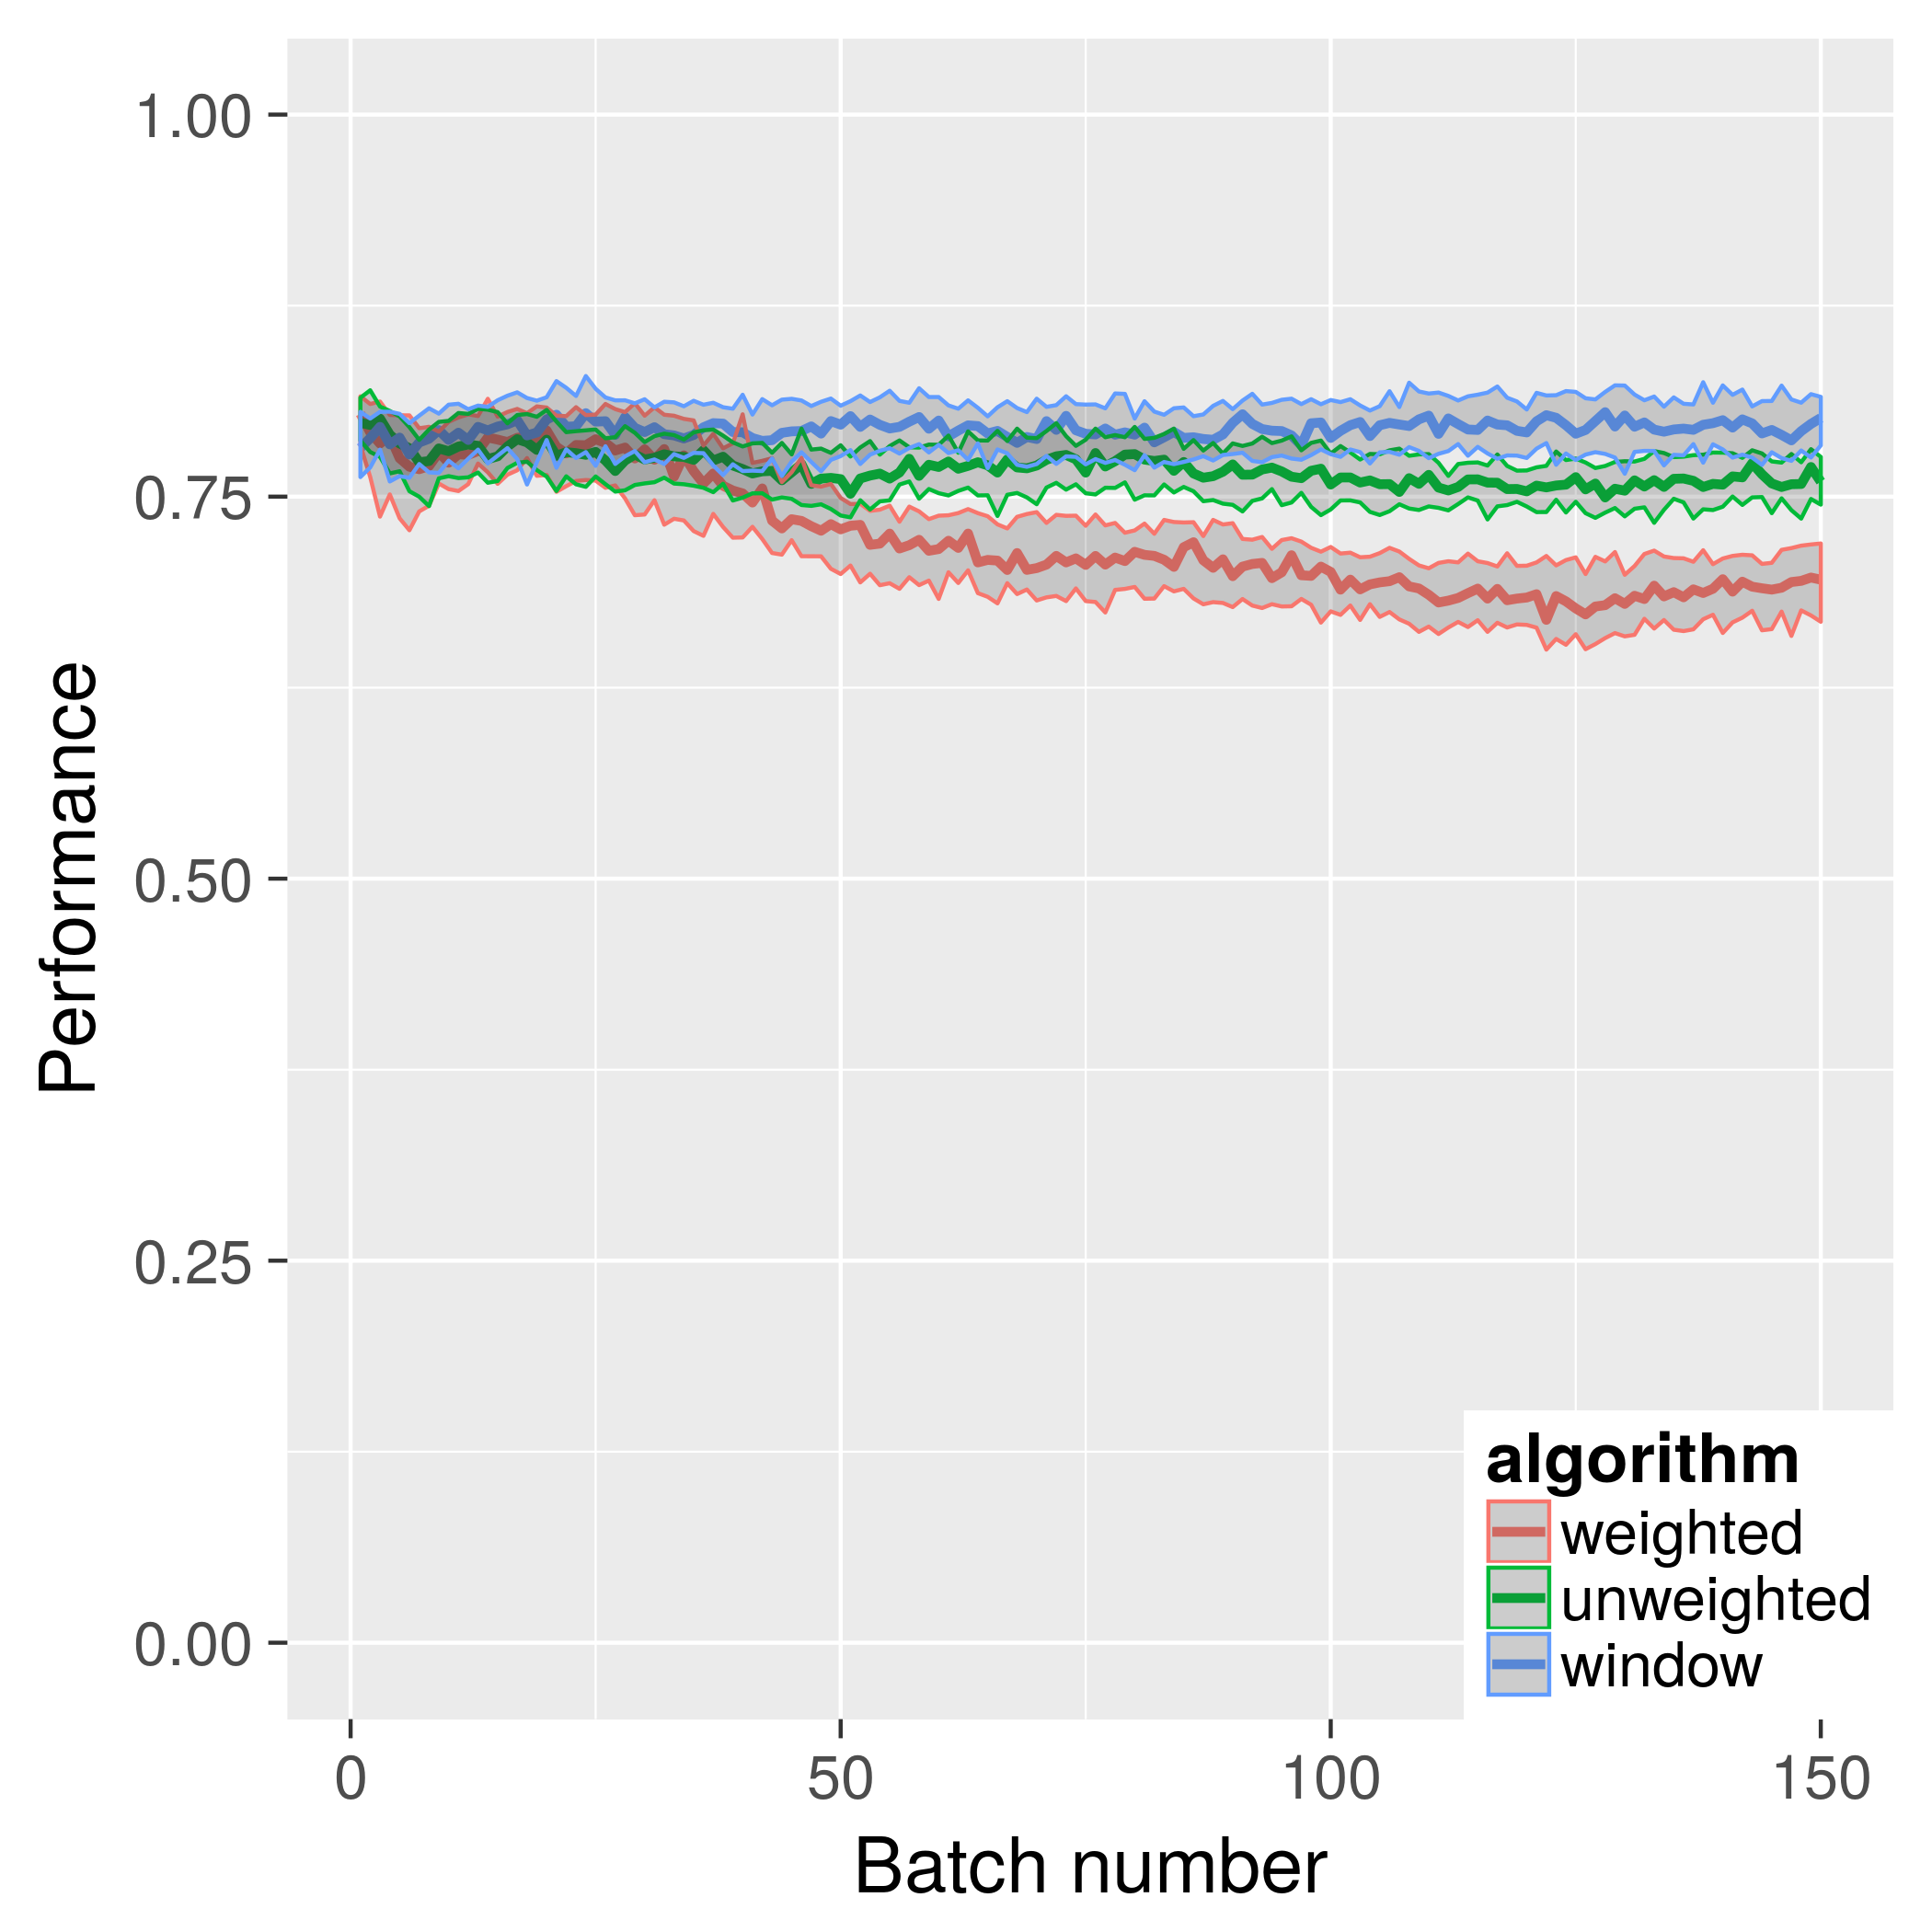
\includegraphics[width=.9\linewidth]{s_set/s_set_3_with_weighted_ci_one_size_vmeasure.png}
  \caption{S3.}
\end{subfigure}%
\begin{subfigure}{.45\textwidth}
  \centering
  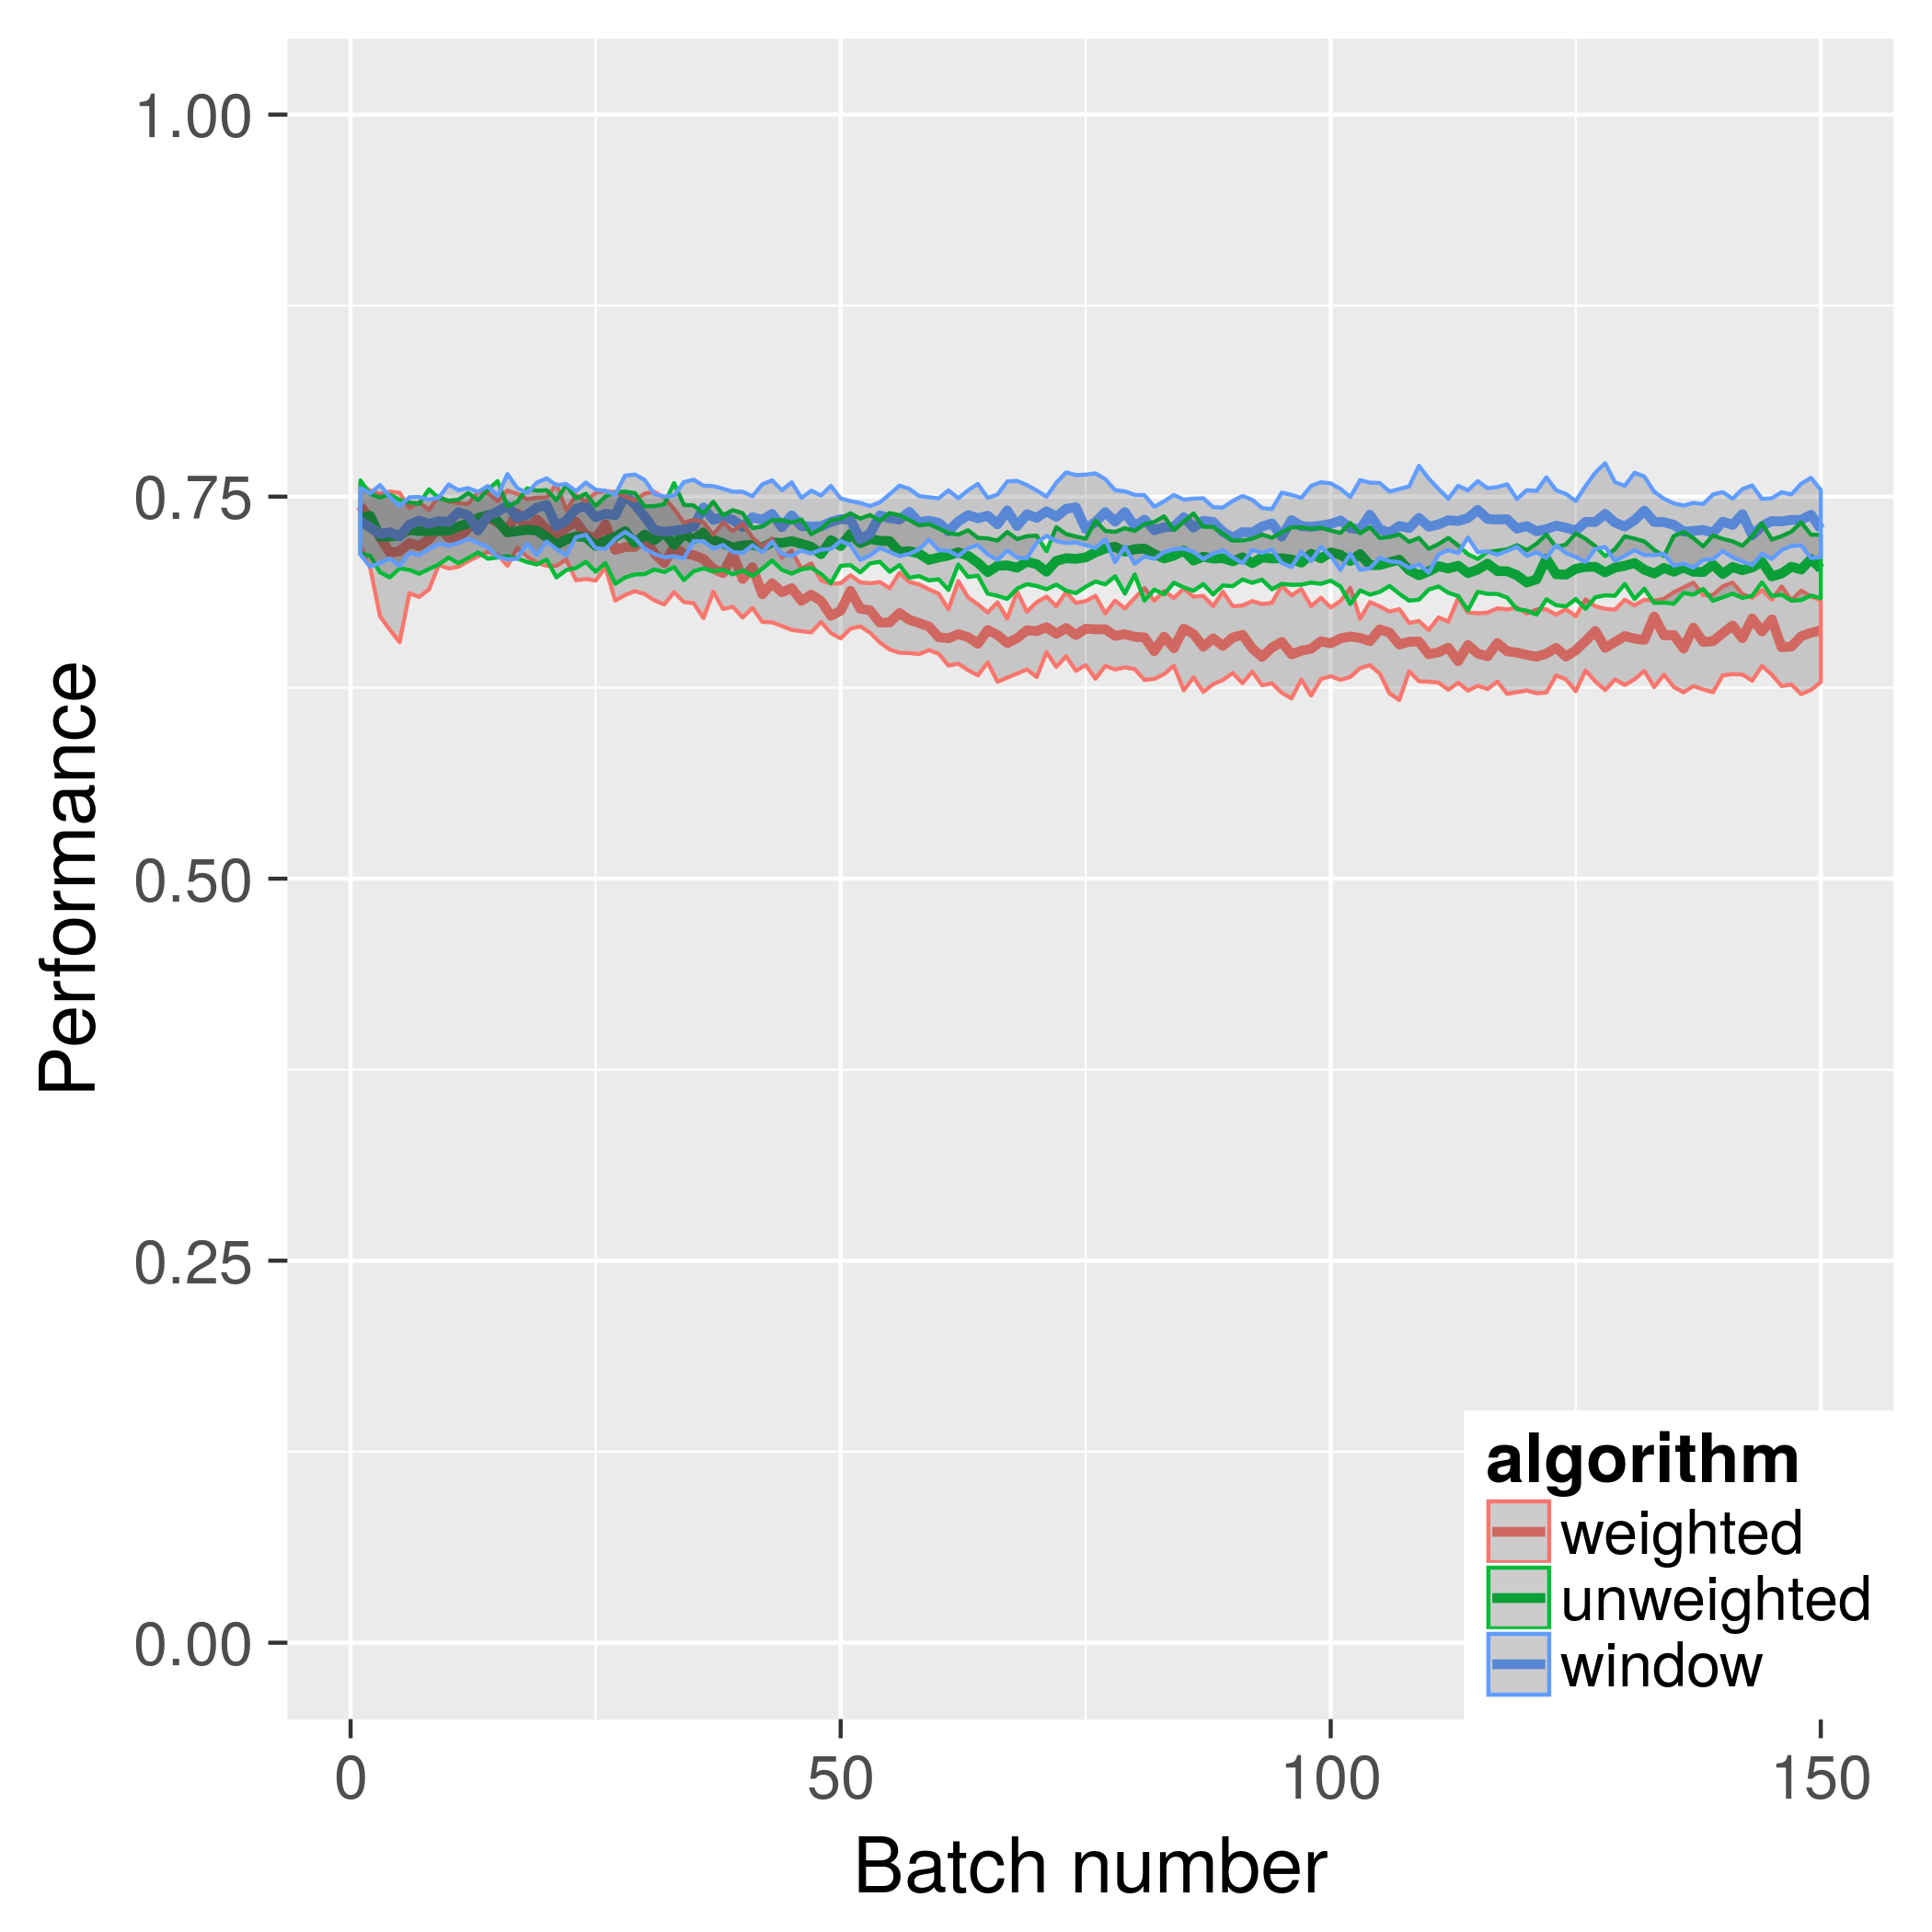
\includegraphics[width=.9\linewidth]{s_set/s_set_4_with_weighted_ci_one_size_vmeasure.png}
  \caption{S4.}
\end{subfigure}
\caption{V-measure for the S data sets.}
\label{fig:s_set_vmeasure}
\end{figure}

Both unweighted spectral CluStream (green) and windowed spectral clustering (blue) perform similarly for all sets.  They both perform well on set S1 and set S2 but they struggle with the more challenging sets S3 and S4.   The weighted spectral CluStream (red) initially starts with performance on par with the competing algorithms, but quickly drops to poor performance and does not recover as the stream progresses. Given that the underlying distributions for the S sets are stationary, this behaviour is unusual.


In order to discover why weighted spectral CluStream is performing poorly, lets look at the micro-clusters more closely. Figure \ref{fig:weighted_issues} shows a snapshot of the weighted spectral CluStream algorithm on the S1 data set in the middle of the stream.

\begin{figure}[h!]
  \centering
  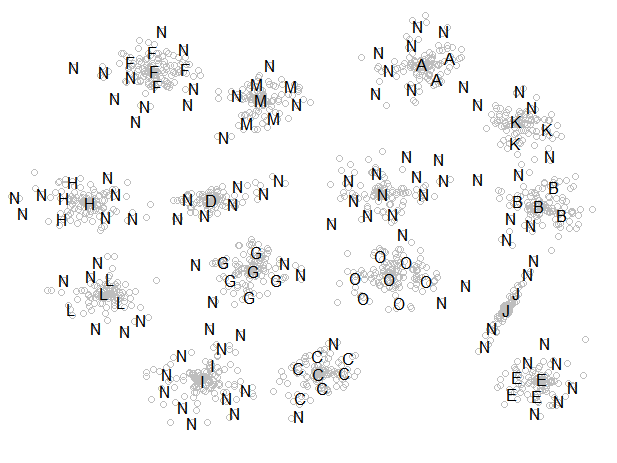
\includegraphics[width = 11cm]{weighted_issues_N_crop}
  \caption{Snapshot from weighted spectral CluStream on S1.}
\label{fig:weighted_issues}
\end{figure}

The grey points are the data points observed so far, the location of the letters represent micro-cluster centres which are labelled with the results of the weighted spectral clustering. This is not a good clustering of the data.  We can see that one cluster (letter N) is dominating and many of the outliers of the other clusters have been represented by the N cluster label. This implies that the affinities between the micro-cluster centres on the outskirts of the cluster C are more similar to the outliers of other clusters (such as cluster I) than to the micro-cluster centres at C. This behaviour is very odd and implies that there might be an issue with the  affinity matrix.



We can observe the affinity matrix by plotting it as an image, where bright values imply an affinity value close to one and red means the value is close to zero. Figure \ref{fig:set_1_affinities} shows an image of both the unweighted and weighted affinity for the example shown in Figure \ref{fig:weighted_issues}. The affinity matrix has dimension $150 \times 150$, with each row representing the similarities between one micro-cluster centre and the other 149. The rows and columns have been grouped so that micro-cluster centres from the same true underlying clusters are next to each other. 

\begin{figure}[h]
  \centering
  \begin{subfigure}{0.45\textwidth}
    \centering
    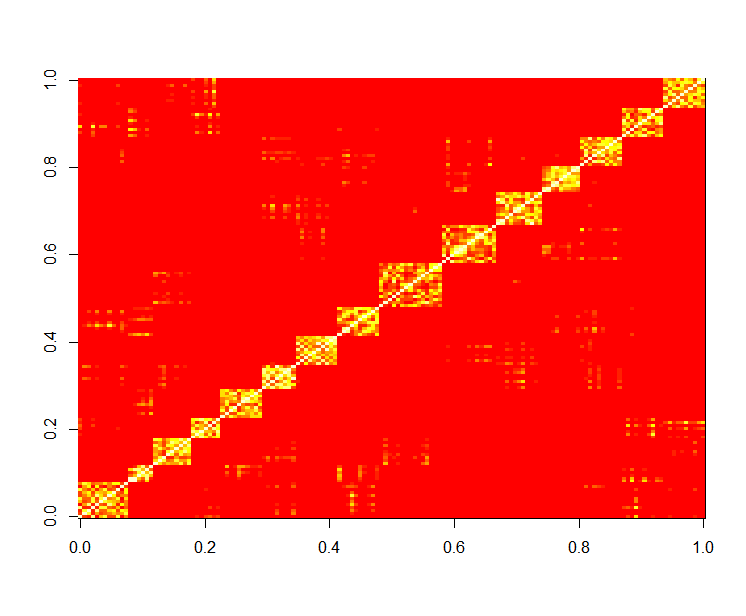
\includegraphics[width = \textwidth, height = \textwidth]{s_set/s_set_1_unweighted_affinity.png}
    \caption{Unweighted affinity matrix.}
  \label{fig:unweighted_affinity}
  \end{subfigure}
  \begin{subfigure}{0.45\textwidth}
    \centering
    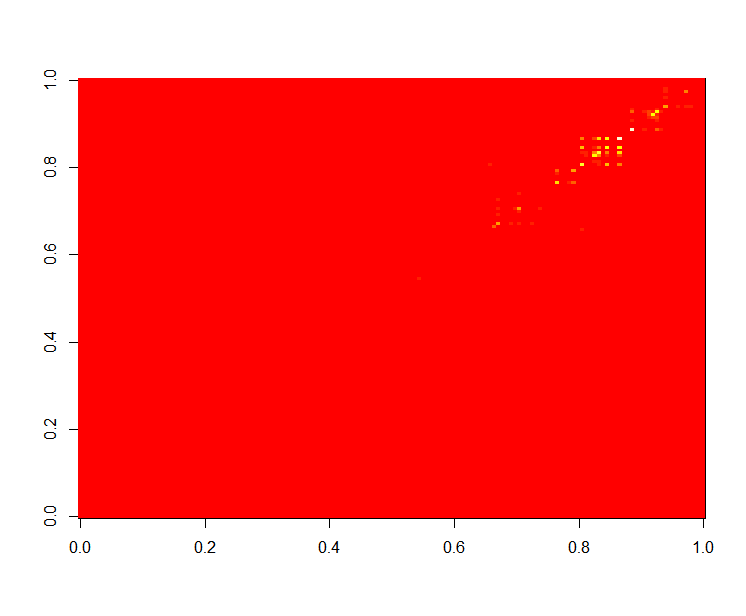
\includegraphics[width = \textwidth, height = \textwidth]{s_set/s_set_1_weighted_affinity.png}
  \caption{Weighted affinity matrix.}
  \label{fig:weighted_affinity}
  \end{subfigure}
    \caption{Affinity matrices for S set 1.}
  \label{fig:set_1_affinities}
\end{figure}

%We can observe the affinity matrix by plotting it as an image, where bright values imply an affinity value close to one and red means the value is close to zero. Figure \ref{fig:set_1_affinities} shows an image of both the unweighted and weighted affinity for the example shown in Figure \ref{fig:weighted_issues}. The affinity matrix has dimension $150 \times 150$, with each row representing the similarities between one micro-cluster centre and the other 149. The rows and columns have been grouped so that micro-cluster centres from the same true underlying clusters are next to each other. 

We can see that in Figure \ref{fig:unweighted_affinity} the block nature of the unweighted affinity is clear. There are strong affinities between close micro-clusters, and weak affinities between distant micro-clusters making this an informative affinity matrix to use with spectral clustering. However in the weighted affinity matrix (Figure \ref{fig:weighted_affinity}) the block nature is not visible. Most of the values are close to zero, with only a few strong affinities. The weighting seems to have dampened the affinity matrix, incorrectly reducing the affinity of  close micro-clusters. It is possible that the use of the localised scaling parameter (see Section \ref{sec:affinity}) in the spectral clustering step may be interfering with the weighting of micro-clusters.  We did attempt to use a global scaling parameter instead of the localised one, however this then brought up the issue of tuning the $\sigma$ parameter, which is known to be very sensitive and is a difficulty for spectral clustering algorithms in general \citep{Luxburg2008}. Although performance did seem to improve with the global scaling parameter when chosen carefully, the performance was still very poor compared to windowed spectral clustering and spectral CluStream.


\subsection{Texture data}

We now investigate the performance of the clustering algorithms features extracted from textured images. The Kylberg  texture data set \citep{kylberg2011c} consists of 28 texture classes with 160 unique texture patches per class. The patches consist of $576 \times 576$ pixel images. Features for clustering were extracted using the LS2W method \citep{Eckley2011} which creates 27 wavelet features from the textured images. 

\begin{figure}[H]
\begin{subfigure}{.15\textwidth}
  \centering
  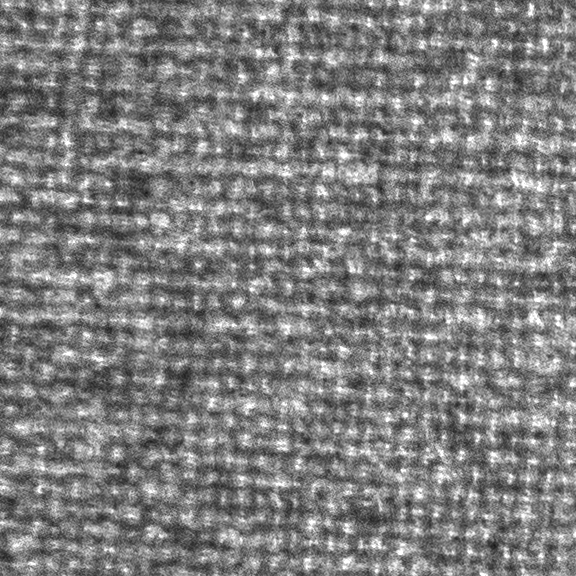
\includegraphics[width=.8\linewidth]{kylberg_examples/blanket1_001.png}
  %\caption{PCA of digits 2 and 9}
 % \label{fig:sfig1}
\end{subfigure}%
\begin{subfigure}{.15\textwidth}
  \centering
  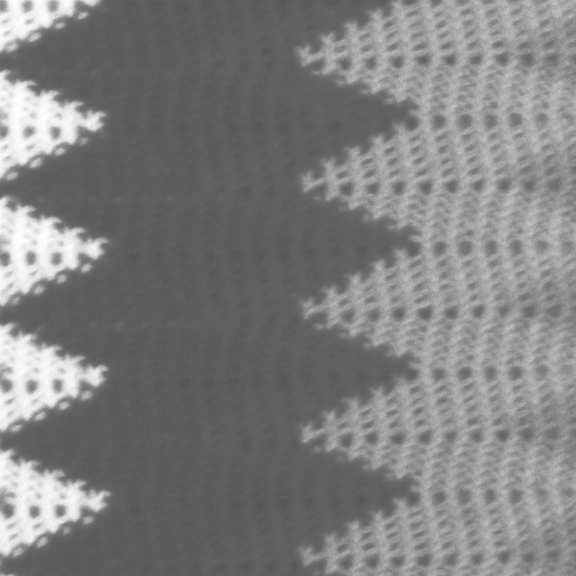
\includegraphics[width=.8\linewidth]{kylberg_examples/blanket2_001.png}
  %\caption{Purity digits 2 and 9}
%  \label{fig:sfig2}
\end{subfigure}
\begin{subfigure}{.15\textwidth}
  \centering
  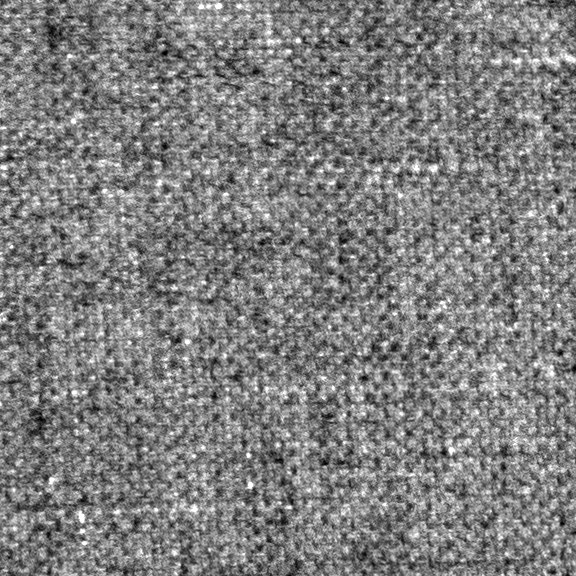
\includegraphics[width=.8\linewidth]{kylberg_examples/canvas1_001.png}
  %\caption{V-measure digits 2 and 9}
%  \label{fig:sfig2}
\end{subfigure}
\begin{subfigure}{.15\textwidth}
  \centering
  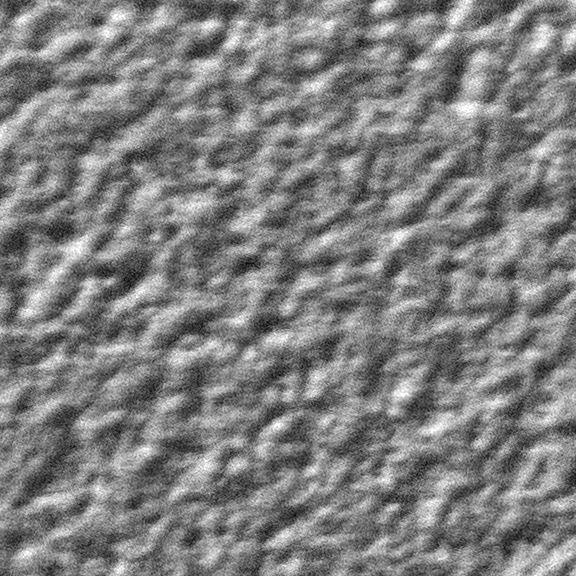
\includegraphics[width=.8\linewidth]{kylberg_examples/ceiling1_001.png}
  %\caption{PCA of digits 2 and 9}
 % \label{fig:sfig1}
\end{subfigure}%
\begin{subfigure}{.15\textwidth}
  \centering
  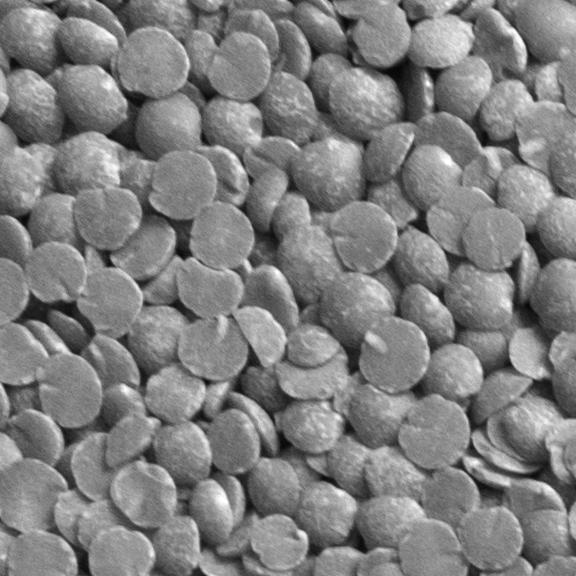
\includegraphics[width=.8\linewidth]{kylberg_examples/lentils1_001.png}
  %\caption{Purity digits 2 and 9}
%  \label{fig:sfig2}
\end{subfigure}
\begin{subfigure}{.15\textwidth}
  \centering
  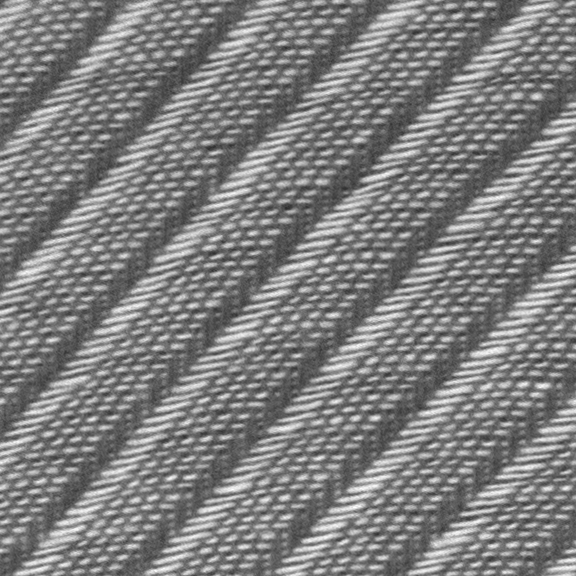
\includegraphics[width=.8\linewidth]{kylberg_examples/screen1_001.png}
  %\caption{V-measure digits 2 and 9}
%  \label{fig:sfig2}
\end{subfigure}

\begin{subfigure}{.15\textwidth}
  \centering
  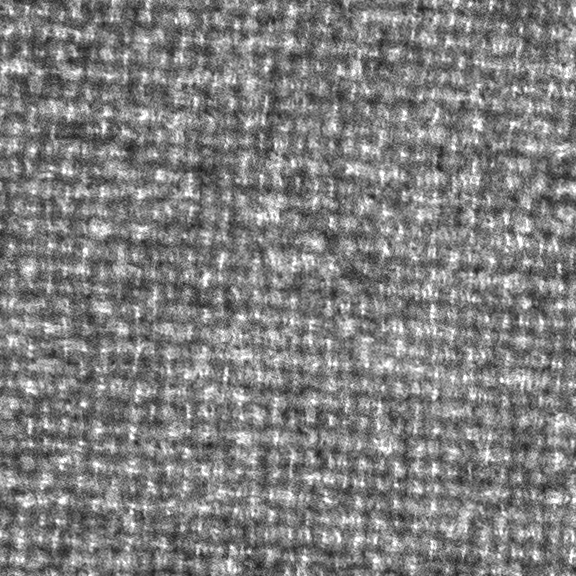
\includegraphics[width=.8\linewidth]{kylberg_examples/blanket1_002.png}
  %\caption{PCA of digits 2 and 9}
 % \label{fig:sfig1}
\end{subfigure}%
\begin{subfigure}{.15\textwidth}
  \centering
  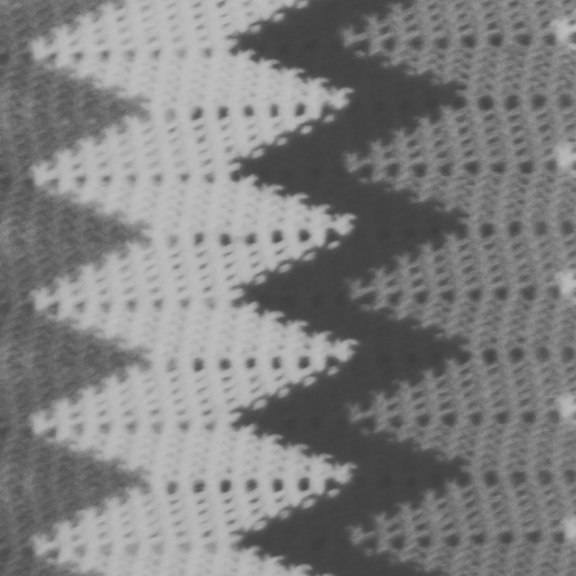
\includegraphics[width=.8\linewidth]{kylberg_examples/blanket2_002.png}
  %\caption{Purity digits 2 and 9}
%  \label{fig:sfig2}
\end{subfigure}
\begin{subfigure}{.15\textwidth}
  \centering
  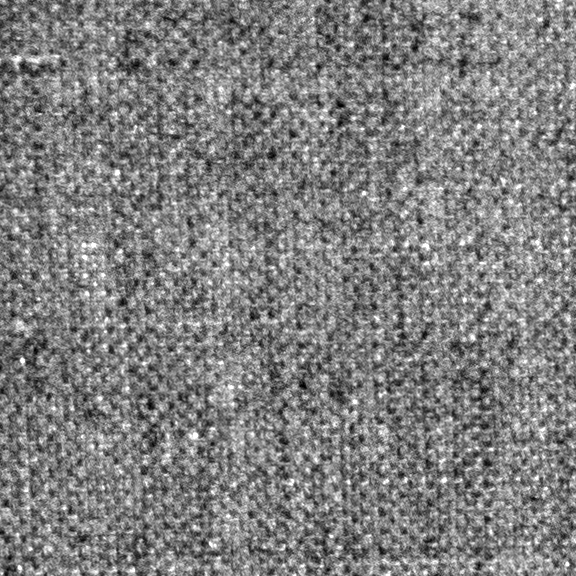
\includegraphics[width=.8\linewidth]{kylberg_examples/canvas1_002.png}
  %\caption{V-measure digits 2 and 9}
%  \label{fig:sfig2}
\end{subfigure}
\begin{subfigure}{.15\textwidth}
  \centering
  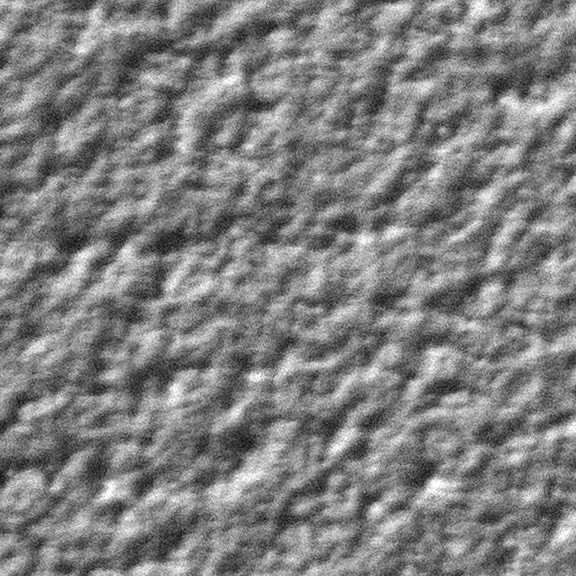
\includegraphics[width=.8\linewidth]{kylberg_examples/ceiling1_002.png}
  %\caption{PCA of digits 2 and 9}
 % \label{fig:sfig1}
\end{subfigure}%
\begin{subfigure}{.15\textwidth}
  \centering
  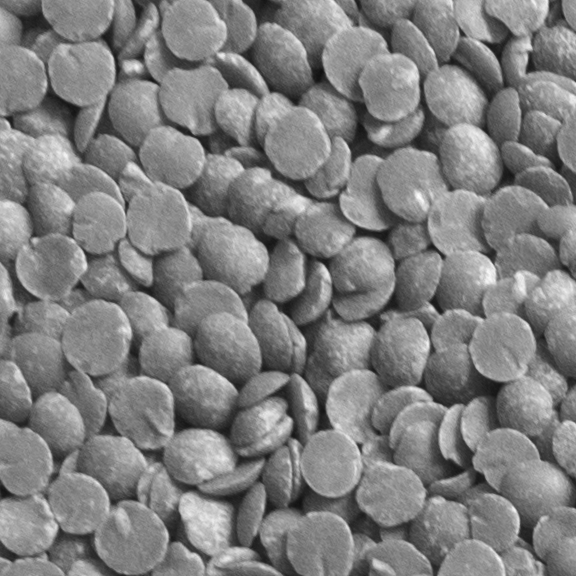
\includegraphics[width=.8\linewidth]{kylberg_examples/lentils1_002.png}
  %\caption{Purity digits 2 and 9}
%  \label{fig:sfig2}
\end{subfigure}
\begin{subfigure}{.15\textwidth}
  \centering
  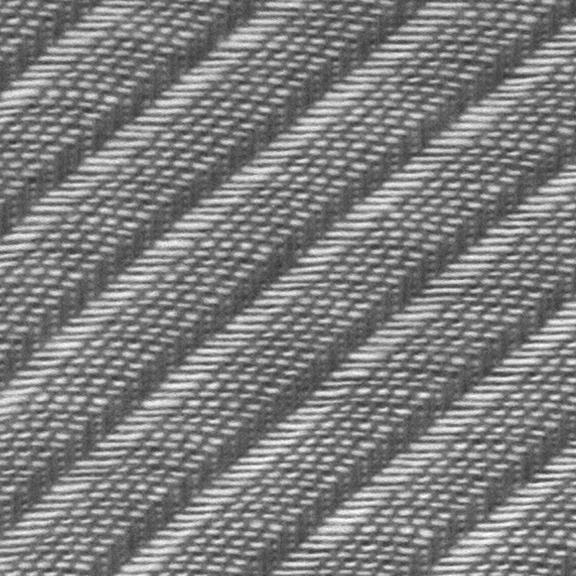
\includegraphics[width=.8\linewidth]{kylberg_examples/screen1_002.png}
  %\caption{V-measure digits 2 and 9}
%  \label{fig:sfig2}
\end{subfigure}

\begin{subfigure}{.15\textwidth}
  \centering
  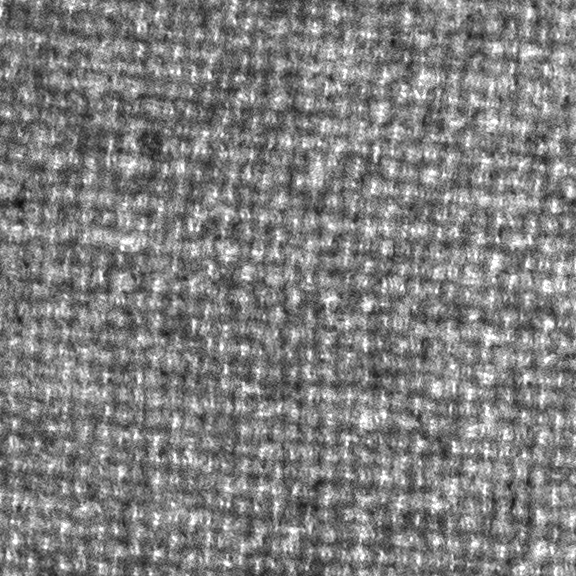
\includegraphics[width=.8\linewidth]{kylberg_examples/blanket1_003.png}
  %\caption{PCA of digits 2 and 9}
 % \label{fig:sfig1}
\end{subfigure}%
\begin{subfigure}{.15\textwidth}
  \centering
  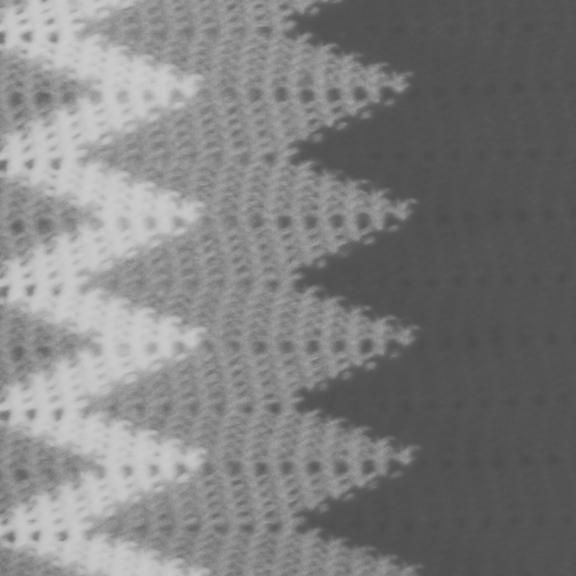
\includegraphics[width=.8\linewidth]{kylberg_examples/blanket2_003.png}
  %\caption{Purity digits 2 and 9}
%  \label{fig:sfig2}
\end{subfigure}
\begin{subfigure}{.15\textwidth}
  \centering
  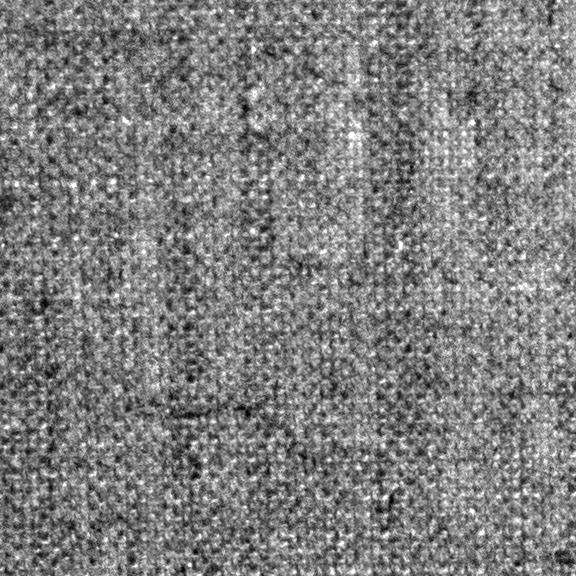
\includegraphics[width=.8\linewidth]{kylberg_examples/canvas1_003.png}
  %\caption{V-measure digits 2 and 9}
%  \label{fig:sfig2}
\end{subfigure}
\begin{subfigure}{.15\textwidth}
  \centering
  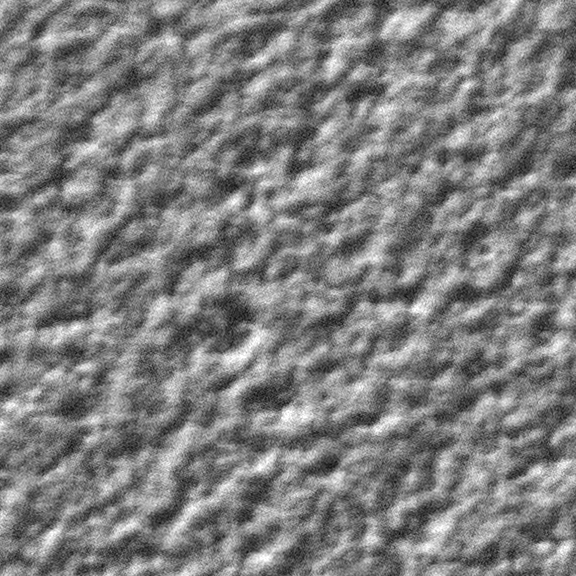
\includegraphics[width=.8\linewidth]{kylberg_examples/ceiling1_003.png}
  %\caption{PCA of digits 2 and 9}
 % \label{fig:sfig1}
\end{subfigure}%
\begin{subfigure}{.15\textwidth}
  \centering
  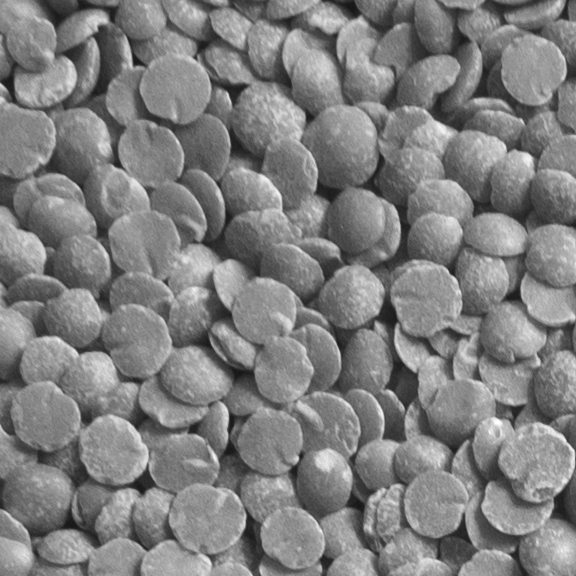
\includegraphics[width=.8\linewidth]{kylberg_examples/lentils1_003.png}
  %\caption{Purity digits 2 and 9}
%  \label{fig:sfig2}
\end{subfigure}
\begin{subfigure}{.15\textwidth}
  \centering
  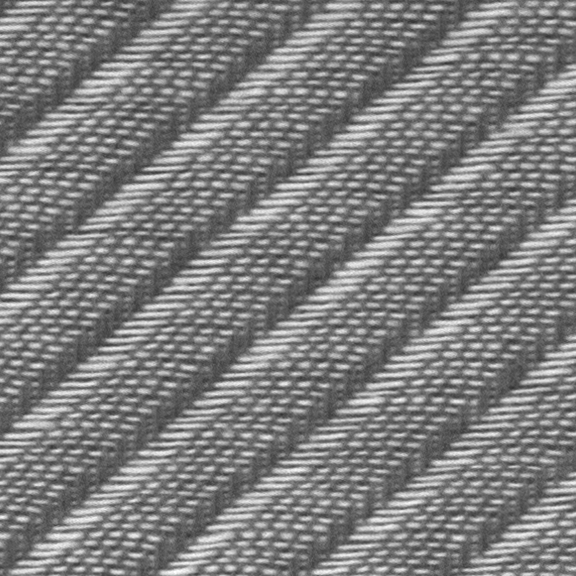
\includegraphics[width=.8\linewidth]{kylberg_examples/screen1_003.png}
  %\caption{V-measure digits 2 and 9}
%  \label{fig:sfig2}
\end{subfigure}
\caption{Three examples from each of the 6 different texture tiles. The texture classes are (L-R) Blanket 1, Blanket 2, Canvas, Ceiling, Lentils and Screen.}
\label{fig:texture_examples}
\end{figure}
A subset of 6 classes was selected,  examples of which are shown in Figure \ref{fig:texture_examples}.  The classes selected are images of two types of blanket, some canvas, a ceiling, some lentils and a screen. The performance plots for the texture data are shown in Figure \ref{fig:texture_results}. Here we  do see a difference between windowed spectral clustering and unweighted spectral CluStream, the windowed approach is generally performing better. Once again weighted spectral CluStream does not perform well, and performance declines as the stream progresses.

\begin{figure}[h!]
\begin{subfigure}{.5\textwidth}
  \centering
  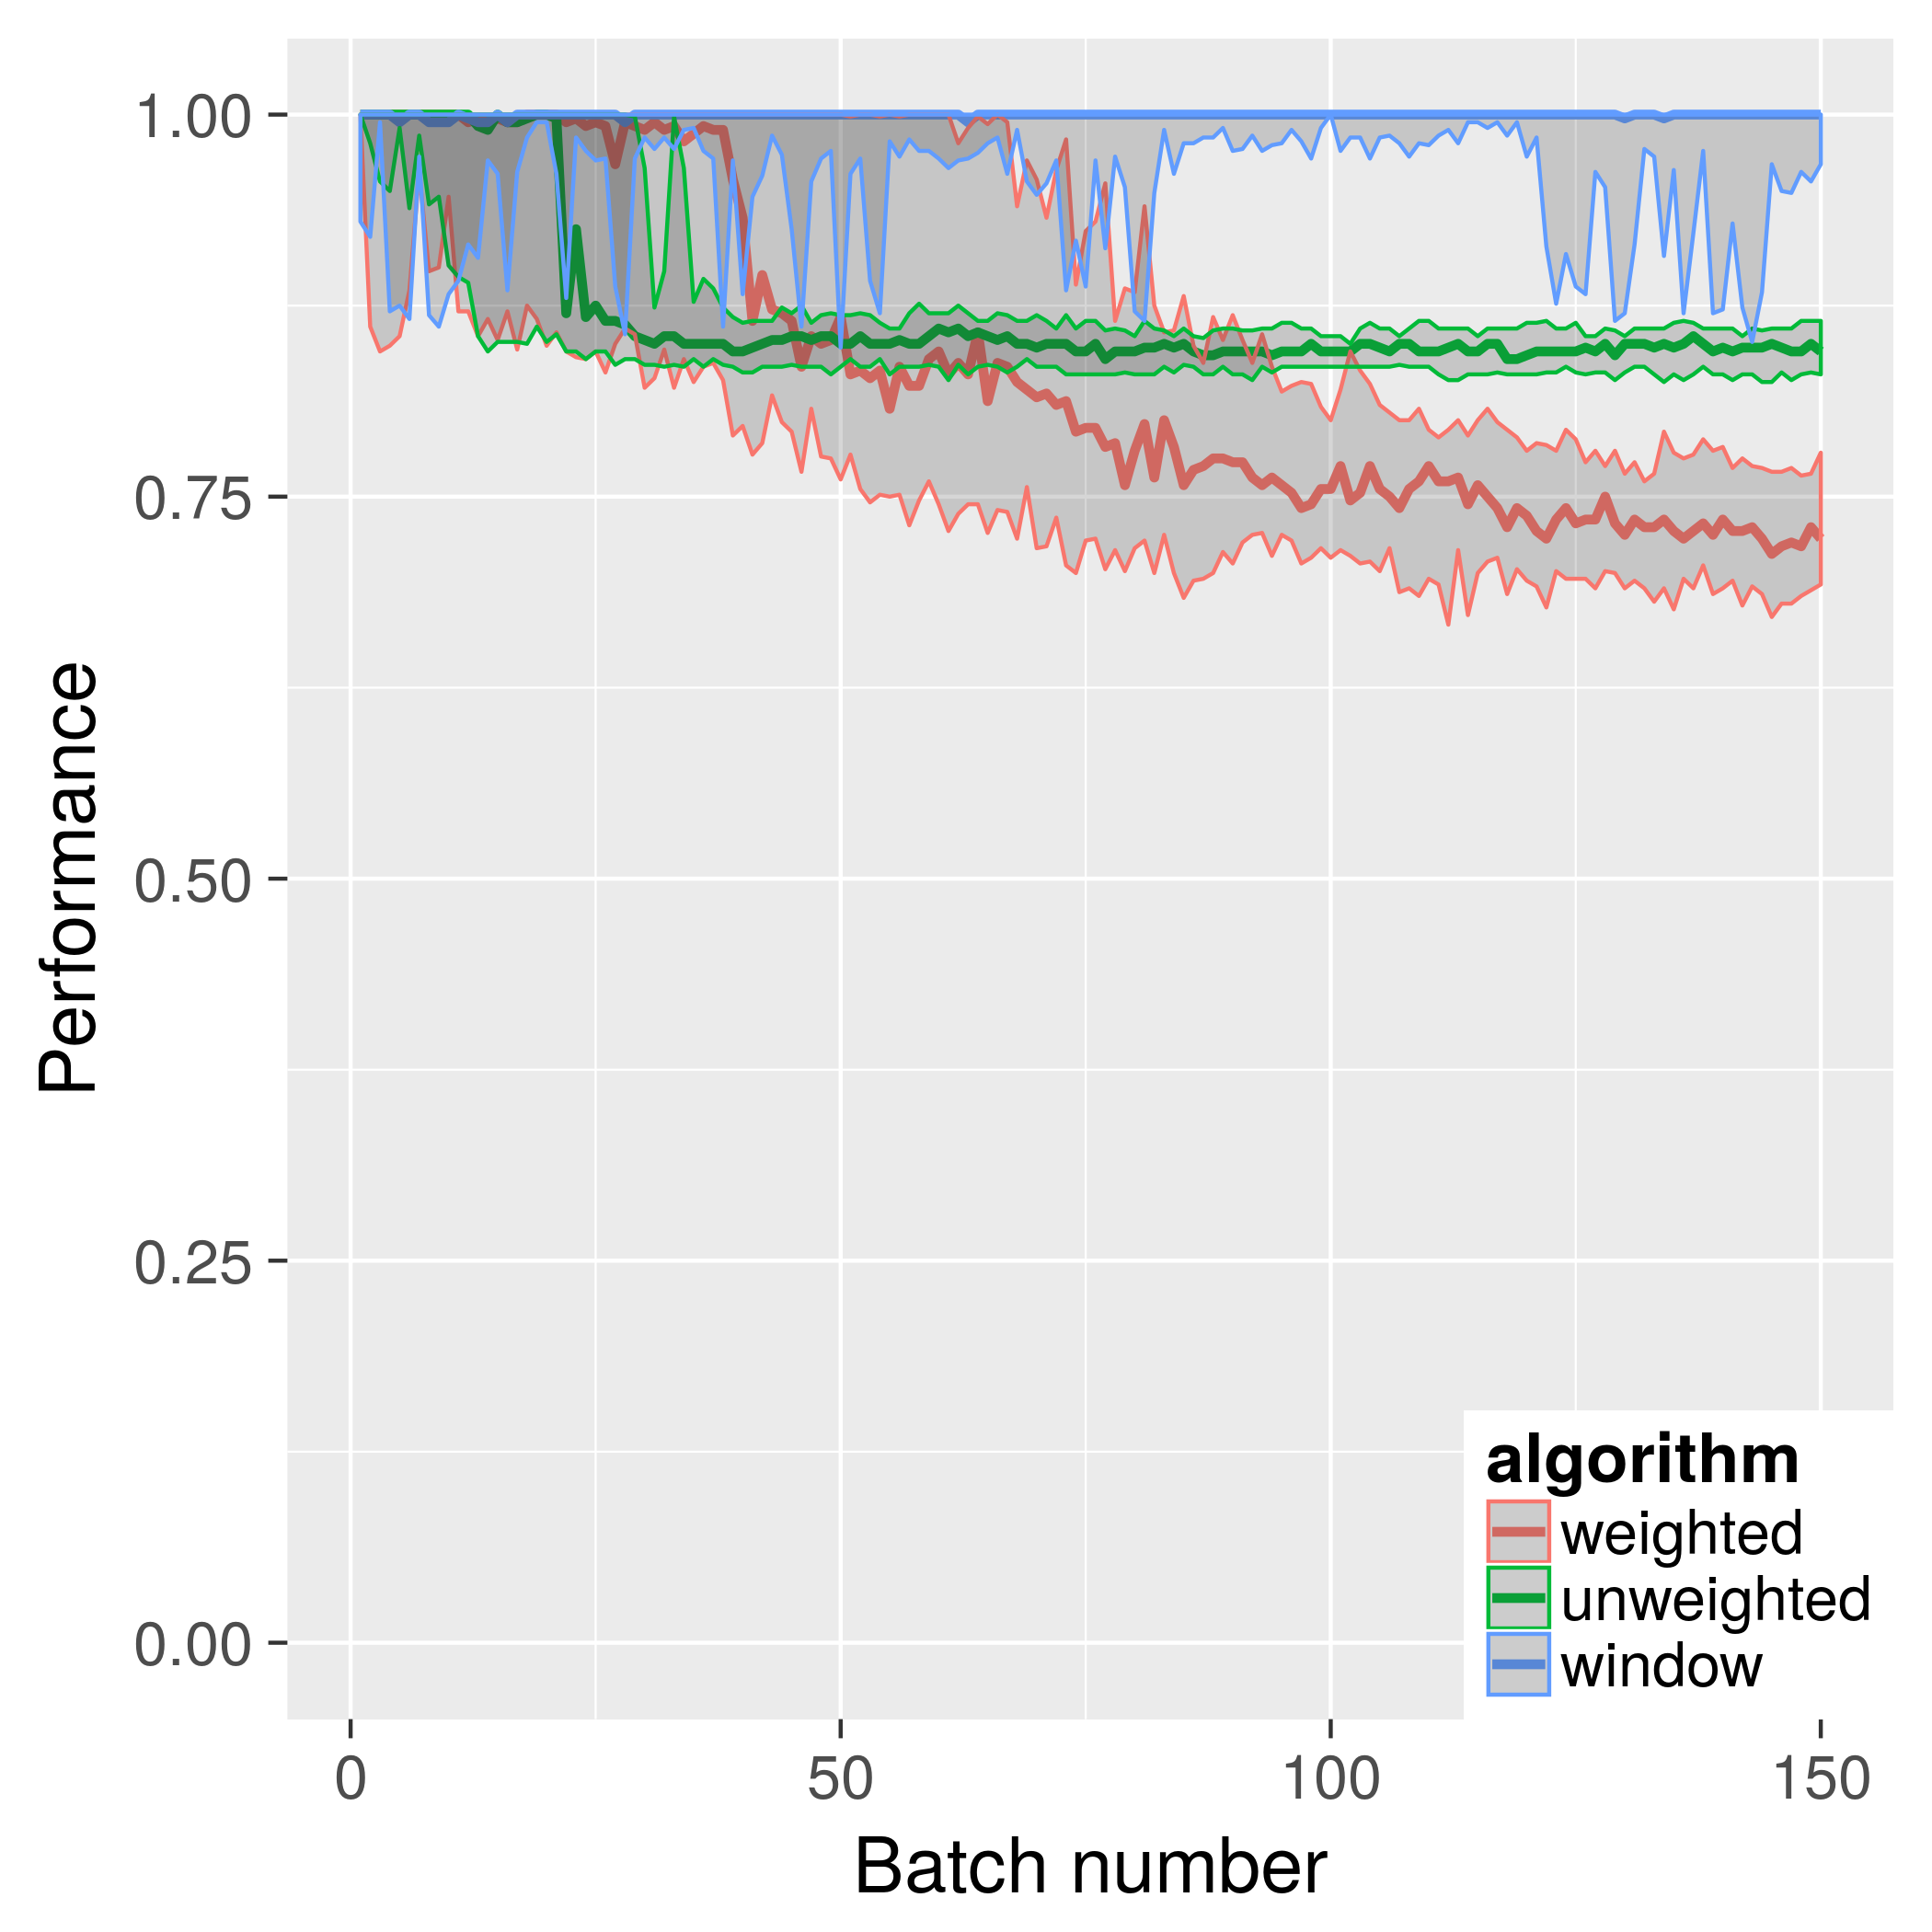
\includegraphics[width=1\linewidth]{texture/texture_with_weighted_ci_one_size_purity}
  \caption{Texture Purity.}
 % \label{fig:sfig1}
\end{subfigure}%
\begin{subfigure}{.5\textwidth}
  \centering
  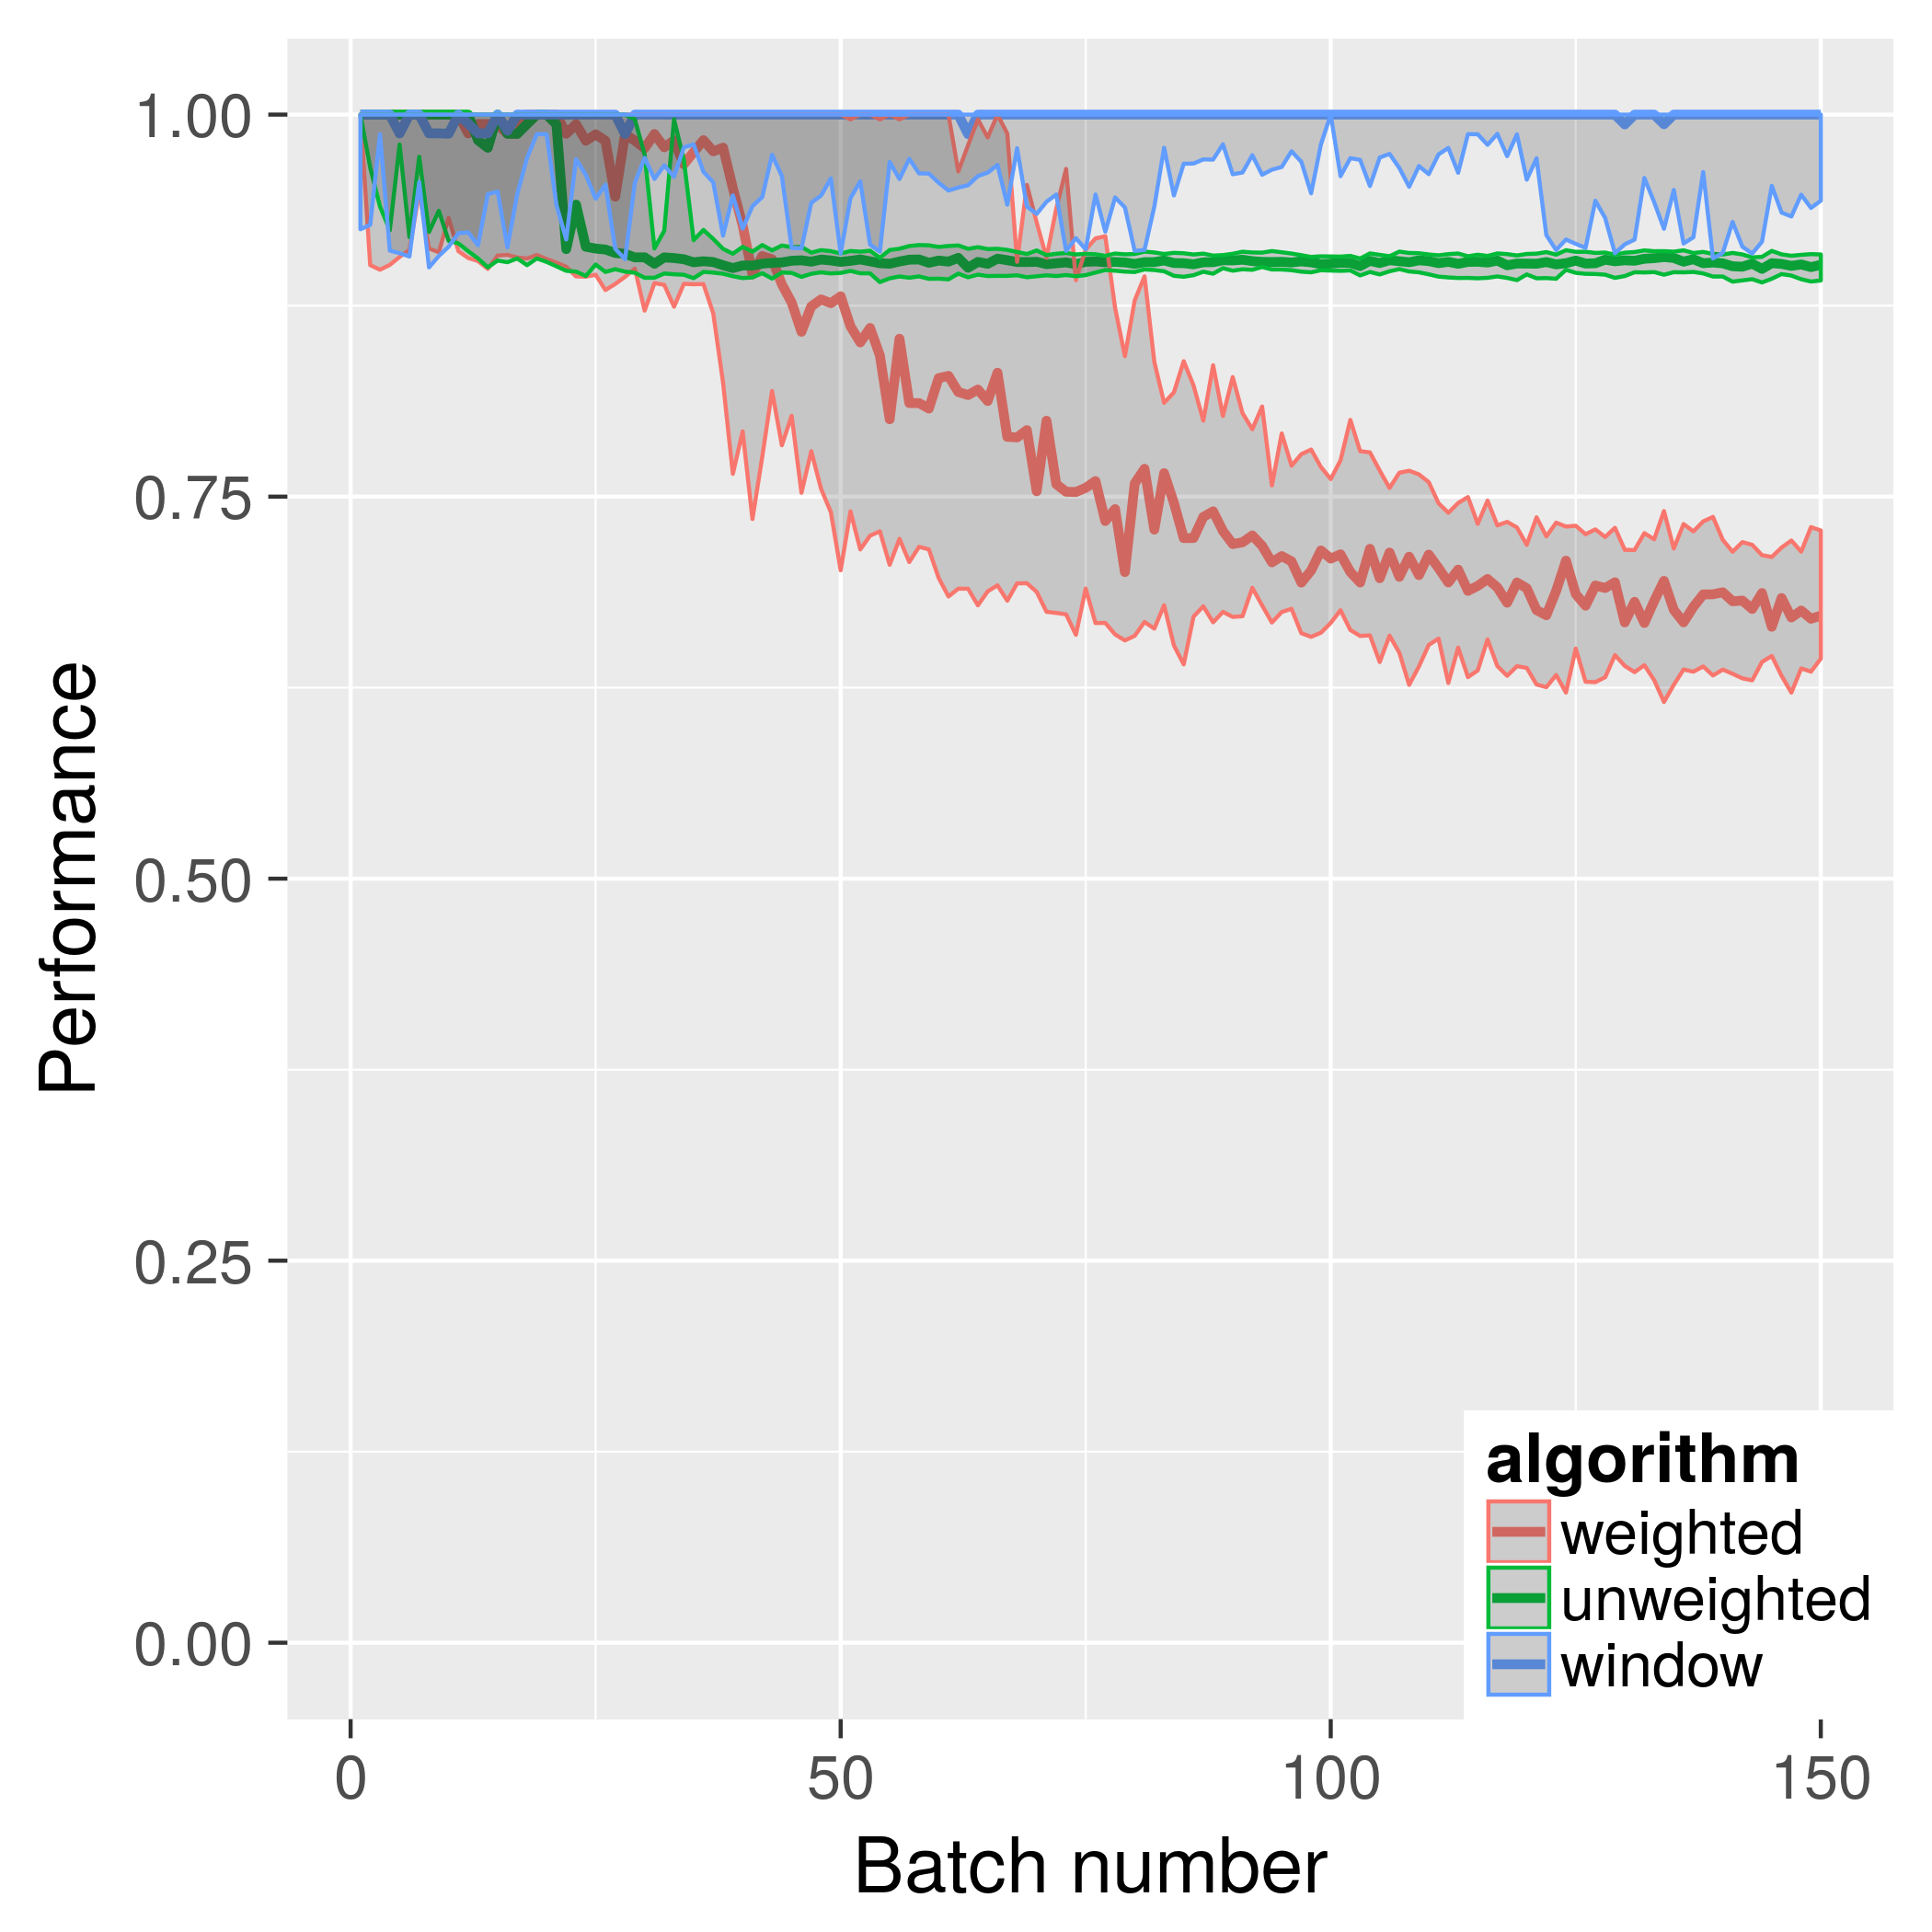
\includegraphics[width=1\linewidth]{texture/texture_with_weighted_ci_one_size_vmeasure}
  \caption{Texture V-measure.}
%  \label{fig:sfig2}
\end{subfigure}
\caption{Texture Results.}
\label{fig:texture_results}
\end{figure}


The poor performance of weighted spectral CluStream was observed on all other data sets investigated and therefore the results from this algorithm  will be dropped from any further performance plots in order to focus more on the behaviour of the other two algorithms.  From now on, we will refer to unweighted spectral CluStream simply as spectral CluStream.
\newpage
\subsection{Pendigit data}
This section and the next will use the UCI Pendigit data set which was introduced in \cite{Alimoglu1996} and is available is for download \citep{Lichman2013}. The data set consists of 250 samples of hand drawn digits of the numbers 0-9 taken from 44 writers. The data was collected using a pressure sensitive tablet. There are 16 features each relating to the co-ordinate information taken from the input tablet. We restrict our analysis to pairwise comparison of digits. For example we attempt to cluster the digits 0 and 1, and treat the data as if it is arriving in a constant data stream.

\begin{figure}[H]

\begin{subfigure}{.3\textwidth}
  \centering
  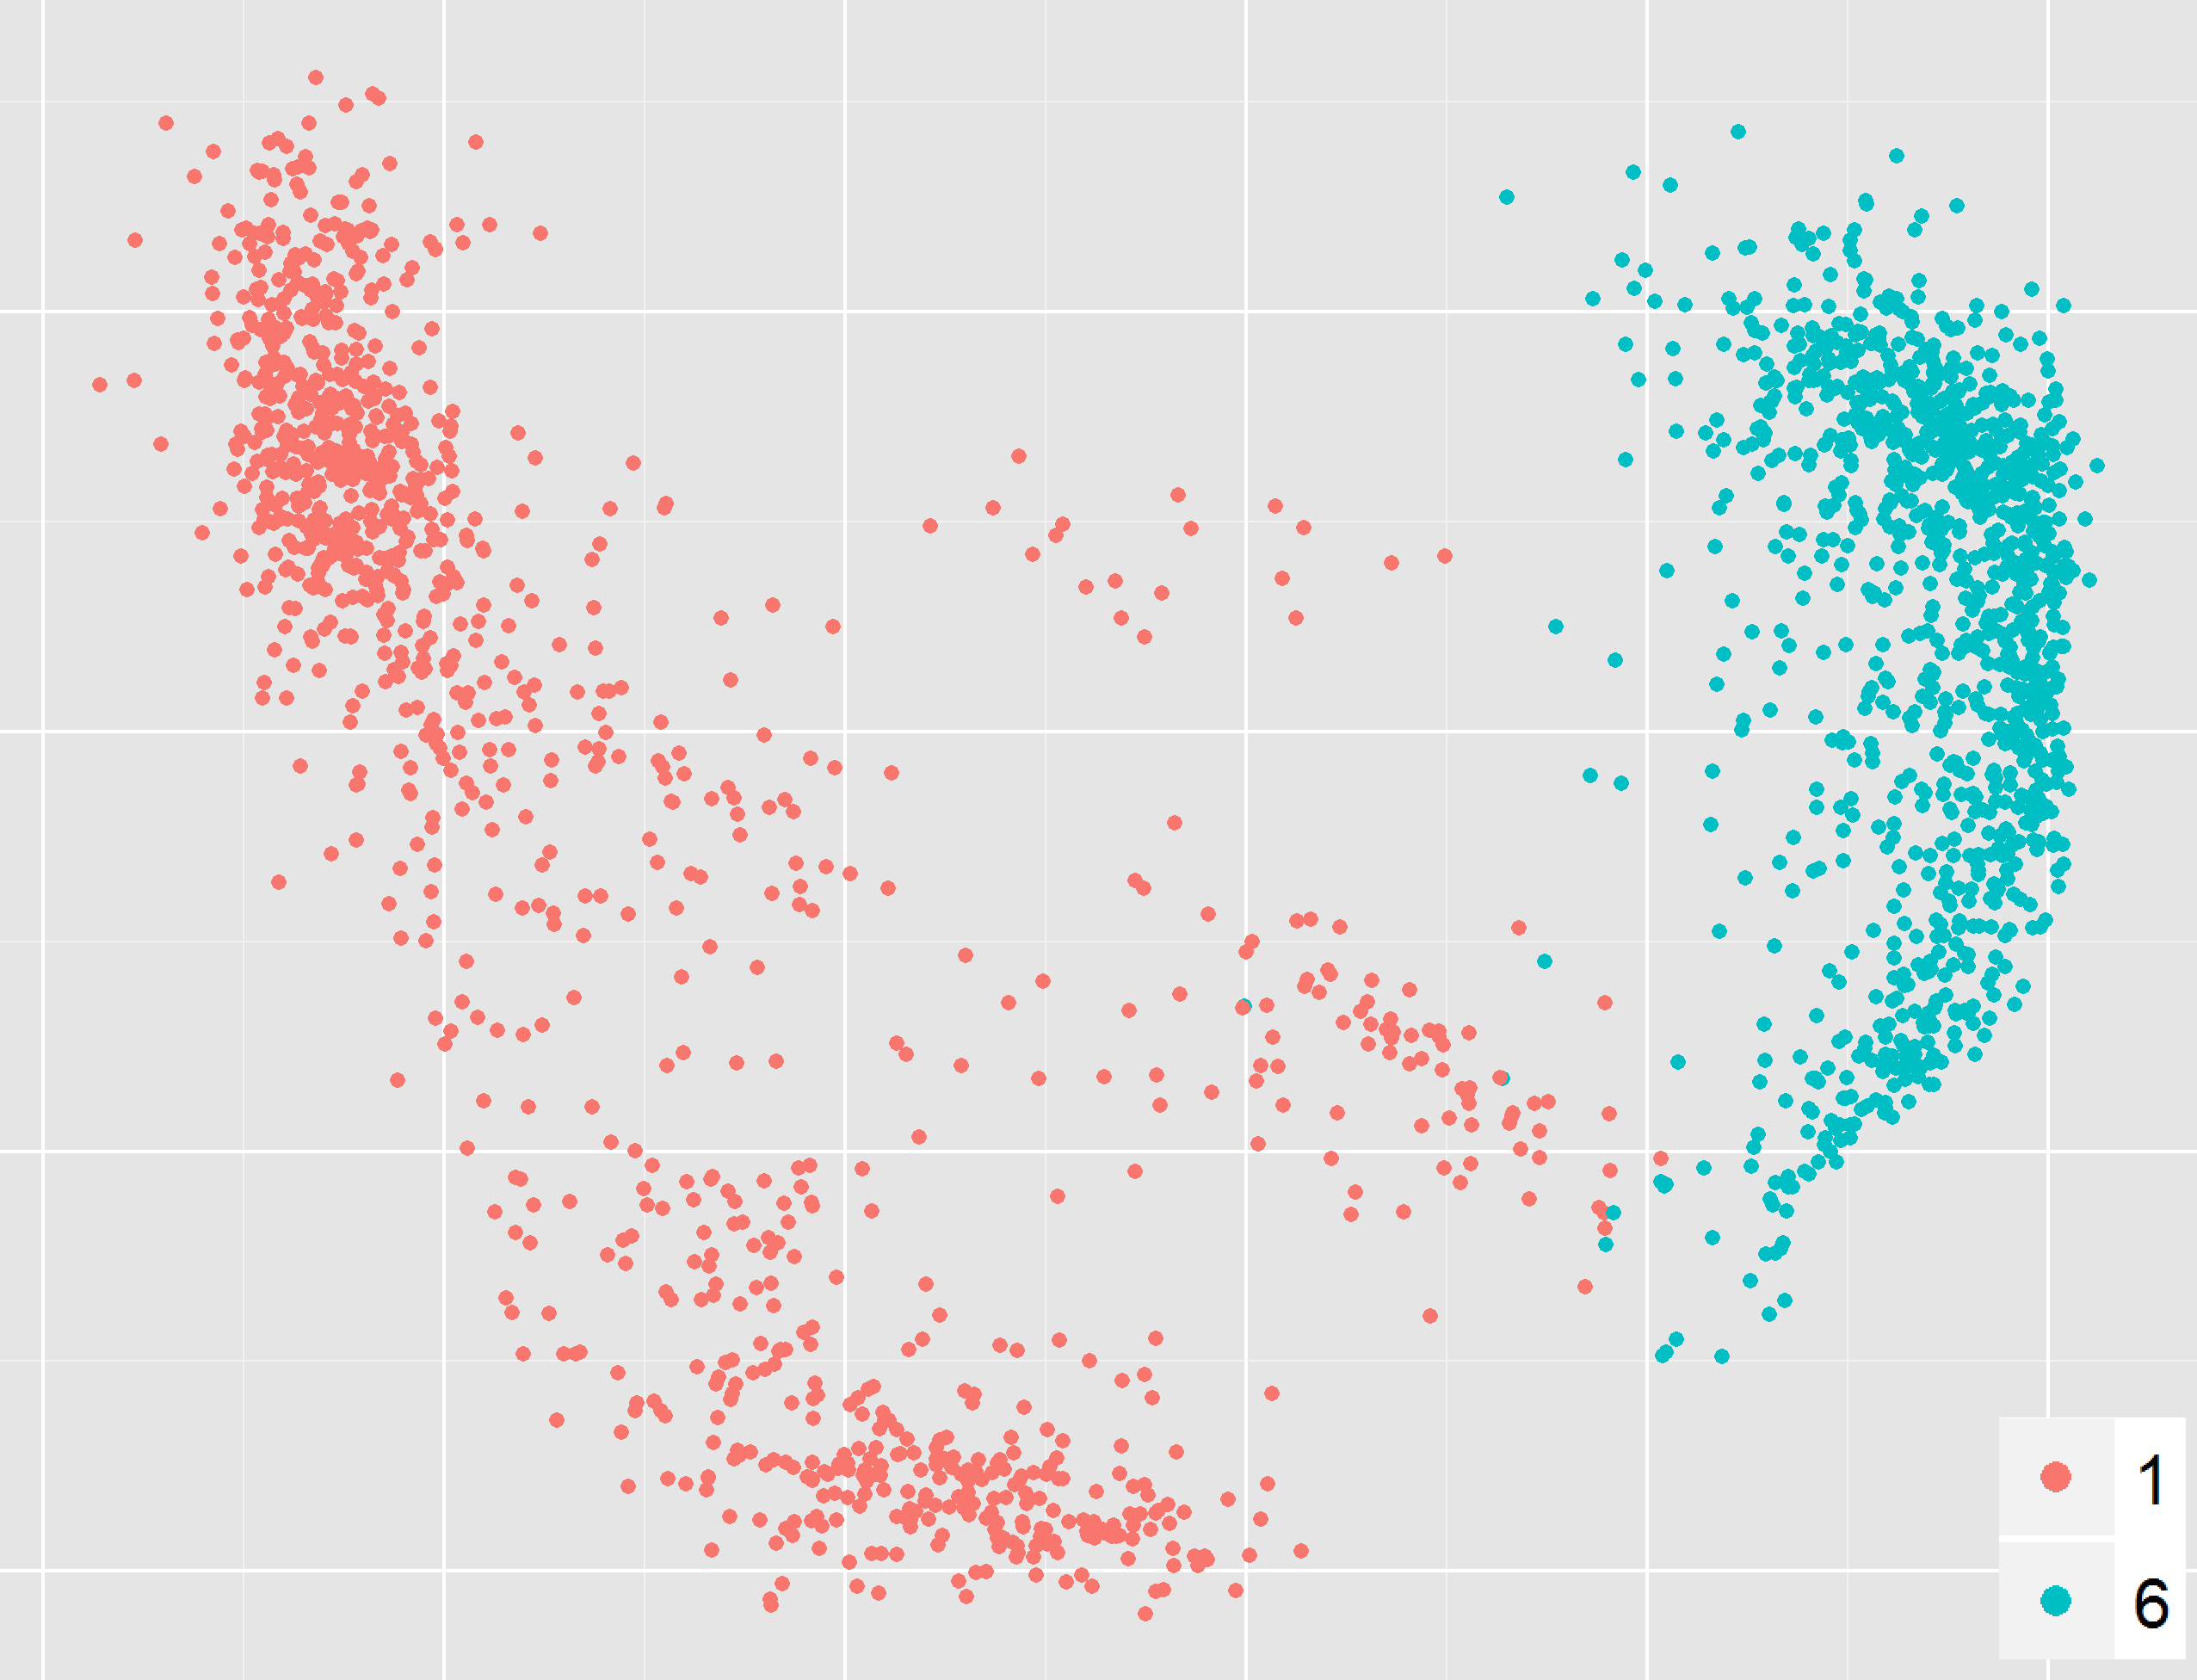
\includegraphics[width=\linewidth]{PCA_pendigits_pairwise/pairwise_1_6_cropped.png}
  \caption{PCA of digits 1 and 6.}
 % \label{fig:sfig1}
\end{subfigure}%
\begin{subfigure}{.3\textwidth}
  \centering
  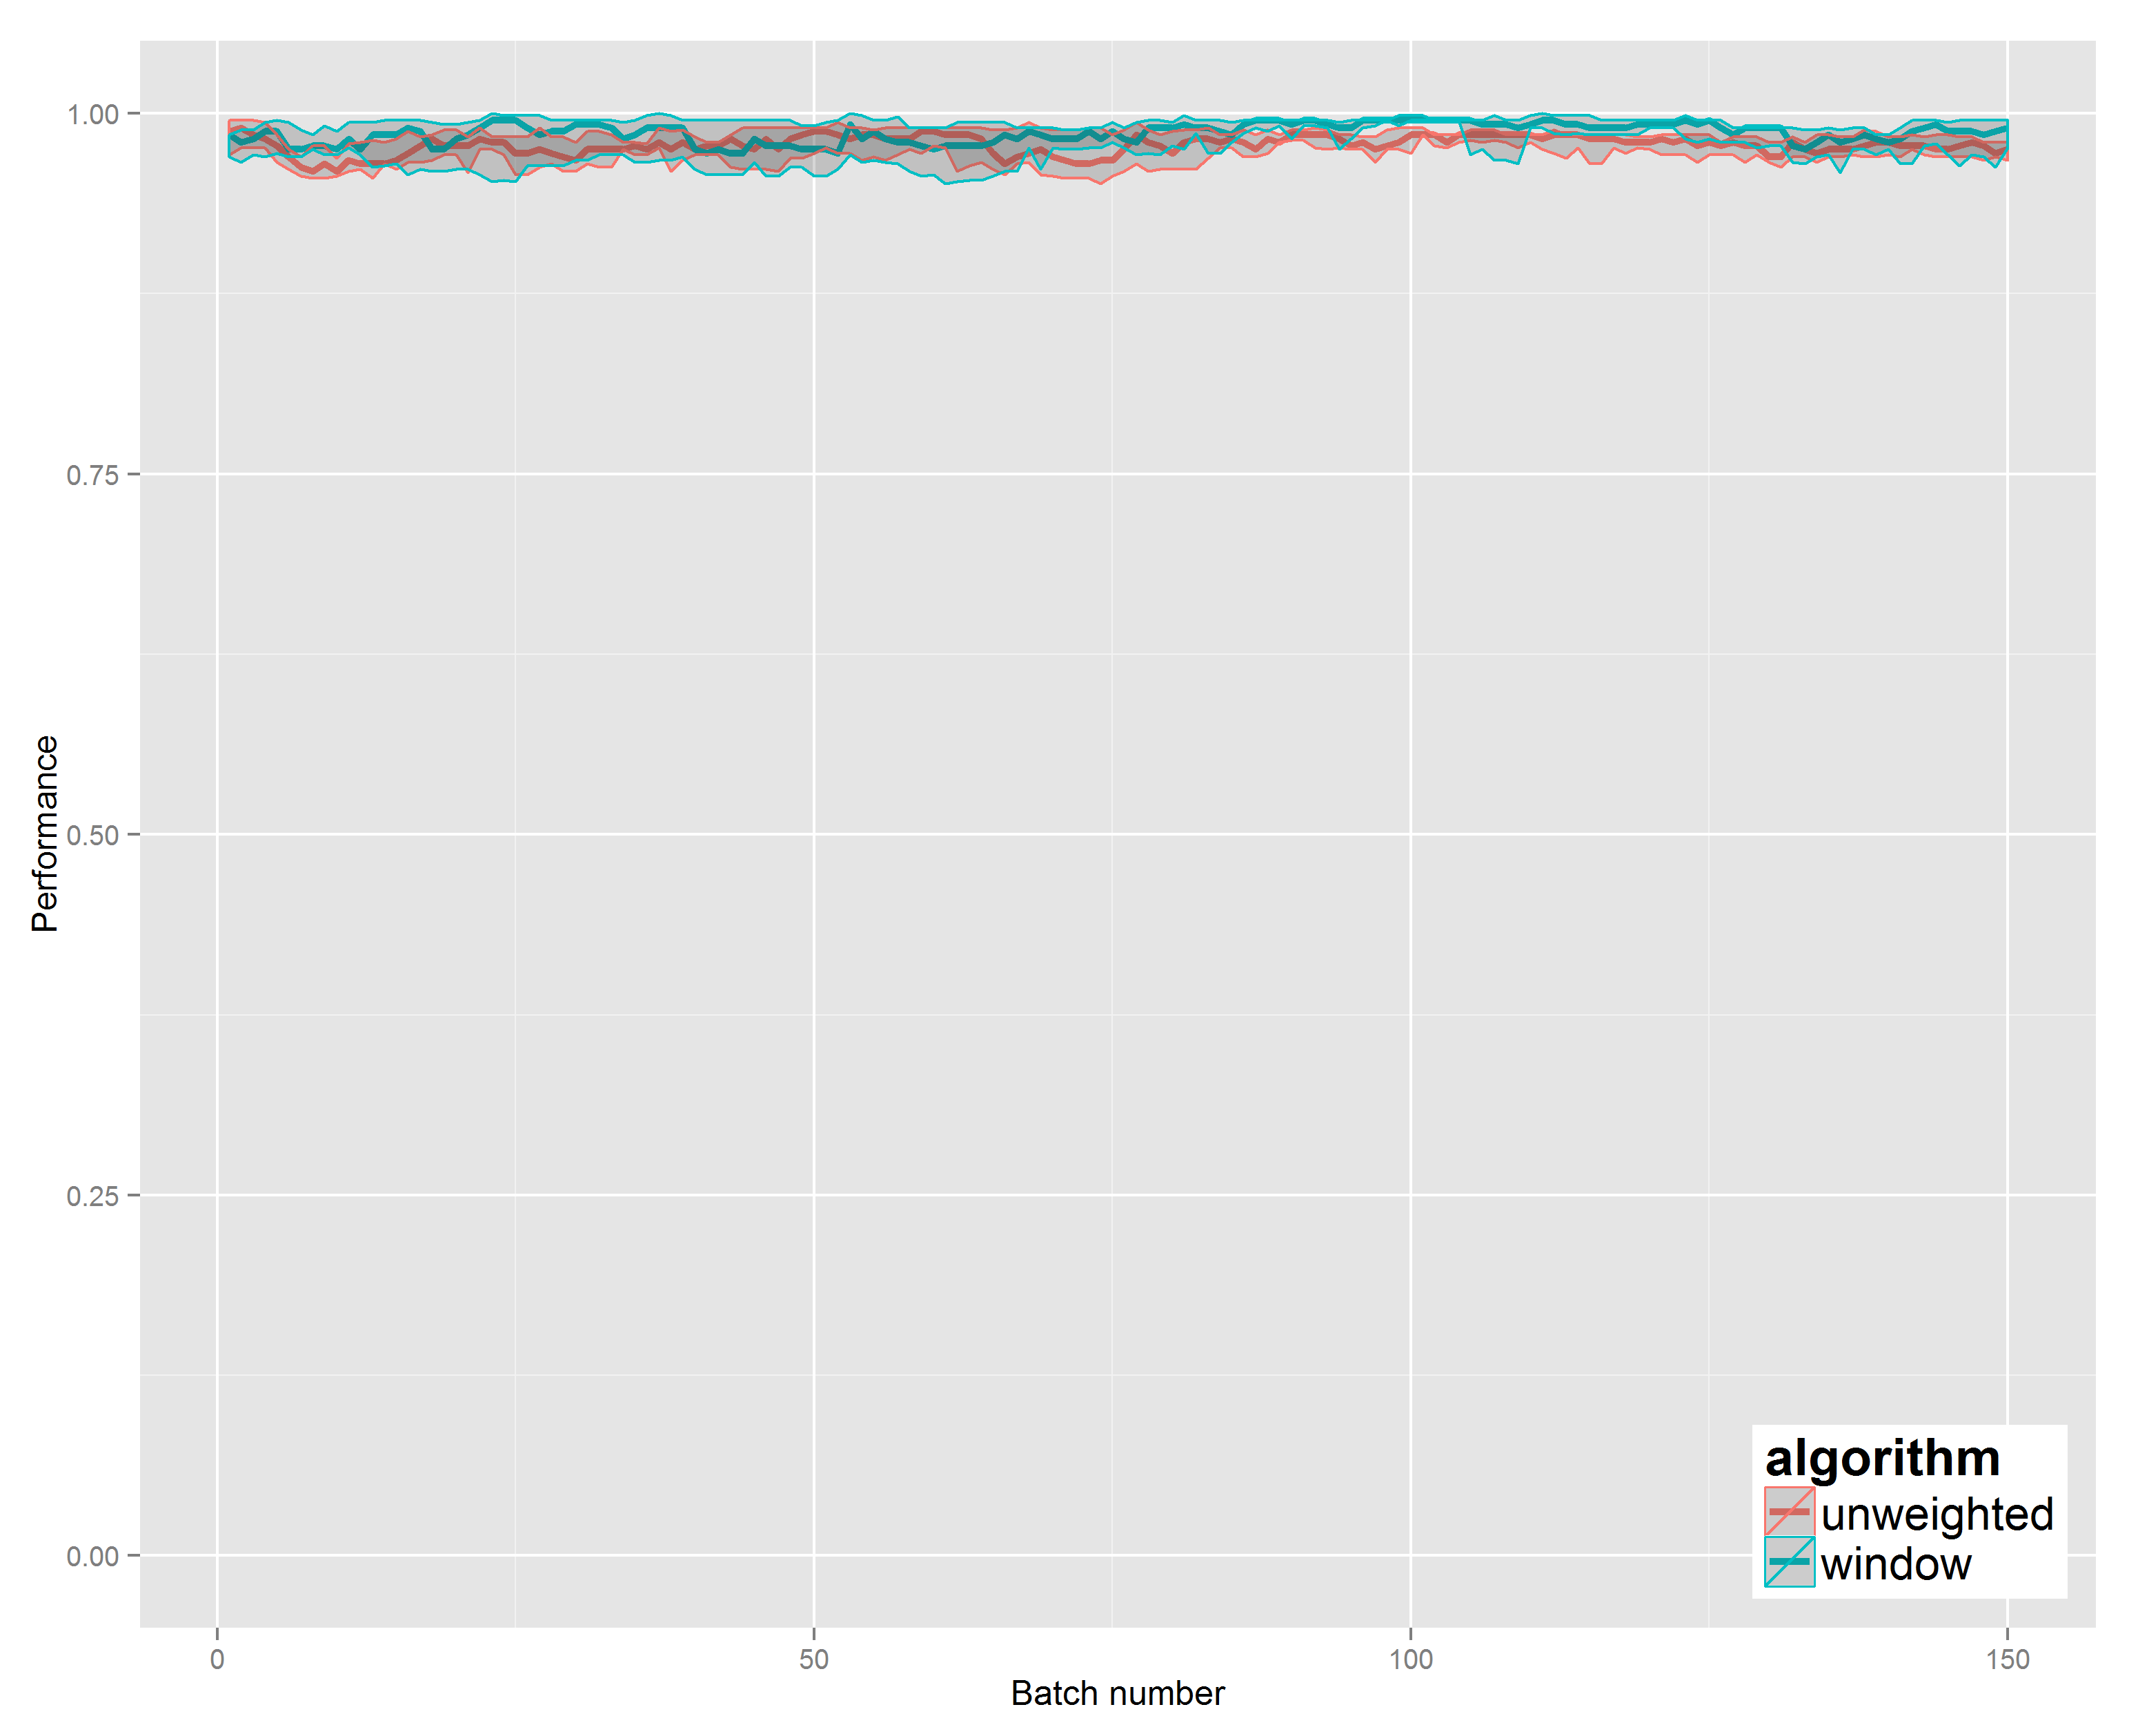
\includegraphics[width=\linewidth]{pendigits_2_alg/uci_pendigits_16_ci_one_size_purity.png}
  \caption{Purity digits 1 and 6.}
%  \label{fig:sfig2}
\end{subfigure}
\begin{subfigure}{.3\textwidth}
  \centering
  \includegraphics[width=\linewidth]{pendigits_2_alg/uci_pendigits_16_ci_one_size_vmeasure.png}
  \caption{V-measure digits 1 and 6.}
%  \label{fig:sfig2}
\end{subfigure}

\begin{subfigure}{.3\textwidth}
  \centering
  \includegraphics[width=\linewidth]{PCA_pendigits_pairwise/pairwise_4_7_cropped.png}
  \caption{PCA of digits 4 and 7.}
 % \label{fig:sfig1}
\end{subfigure}%
\begin{subfigure}{.3\textwidth}
  \centering
  \includegraphics[width=\linewidth]{pendigits_2_alg/uci_pendigits_47_ci_one_size_purity.png}
  \caption{Purity digits 4 and 7.}
%  \label{fig:sfig2}
\end{subfigure}
\begin{subfigure}{.3\textwidth}
  \centering
  \includegraphics[width=\linewidth]{pendigits_2_alg/uci_pendigits_47_ci_one_size_vmeasure.png}
  \caption{V-measure digits 4 and 7.}
%  \label{fig:sfig2}
\end{subfigure}
\caption{Pendigits Pairwise - spectral CluStream and windowed spectral clustering.}
\label{fig:uci_pendigits}
\end{figure}

The results for a selection of the pairwise digits are shown in Figure \ref{fig:uci_pendigits}. The first column displays the digit data in PCA space, the second column shows the purity, and the third column shows the V-measure. Both algorithms show similar performance in the plots shown (and in all the other pairwise combinations which were run).  It can be noted that V-measure is lower than purity, which might imply that the resulting clusters are homogeneous but not complete (see Section \ref{sec:performance}). 



\subsection{Non-stationary data}
\label{sec:non_stationary}

So far we have considered only stationary data streams. The main challenge for clustering algorithms for data streams is adapting to changes in the data stream. In order to create data streams with a non stationary distribution we introduce a change into the data stream. To construct a data stream we choose three digits in the Pendigits data set (for example 4, 8 and 9). The start of the data stream consists only of 2 digits (4 and 8). Half way through the stream, we replace  the second digit with the third digits (so now we observe values 4 and 9 rather than 4 and 8). By swapping the digits in this manner we can avoid the difficult issue of having to select a number of clusters, as we always observe only two clusters.

\begin{figure}[h]
  \centering
 \includegraphics[width=.5\linewidth]{evolving_pen/evolving_pen_48_49_truth.png}  
\caption{PCA plot for the Pendigits 4, 8 and 9.}
\label{fig:48_49_pca}
\end{figure}

The example set is ``Pendigits 48 49'' - first we observe features from digits 4 and 8, and we switch to observing features from digits 4 and 9 half way through the stream. Figure \ref{fig:48_49_pca} shows the PCA space for all  three digits. There is quite a bit of overlap between digits 4 and 9, which makes the data stream quite tricky to cluster. We ran spectral CluStream and windowed spectral clustering on this  data stream. We have included a number of different values for the number of micro-clusters  $q \in (50, 100, 150, 200)$ and also ran windowed spectral with window sizes $w \in( 50,100,150, 200)$. The results in terms of purity and V-measure are shown in Figure \ref{fig:results_48-49}. 
In Figure \ref{fig:results_48-49} the dashed lines show the windowed spectral clustering and the full lines are unweighted spectral CluStream. The colours indicate different values for the number of micro-clusters/window size. 

%Due to the nature of algorithms with windowing, we would expect windowed spectral clustering to adapt quickly to this change given the window size is fairly small ($w = 150$). The initial results showed spectral CluStream performing poorly after the change, and struggling to recover. These results will be shown at the end of the section, and fix is suggested to correct the poor behaviour. First, in order to understand why spectral CluStream was performing badly lets consider a specific example. 

%%%%%%%
\begin{figure}[!h]
        \centering
        \begin{subfigure}[b]{0.47\textwidth}
          \includegraphics[width=\textwidth]{standard_alt/evolving_pen_48_49_standard_purity.png}   
                 \caption{Purity.}
                 \label{fig:p_4849}
        \end{subfigure}
        \begin{subfigure}[b]{0.47\textwidth}
          \includegraphics[width=\textwidth]{standard_alt/evolving_pen_48_49_standard_vmeasure.png}
                 \caption{V-measure.}
                 \label{fig:v_4849}
        \end{subfigure}
\caption{Purity and V-measure for  Pendigits 48-49.}
\label{fig:results_48-49}
\end{figure}

The initial results show that spectral CluStream does not perform well after the change is observed. Both purity and V-measure drop dramatically low and do not recover. A fix is required in order for spectral CluStream to deal with the change in the data stream. In order to understand why performance drops at the change and discover how to fix this we need to look closely at the behaviour of the  micro-clusters. Figure \ref{fig:stream_1} shows the micro-clusters for spectral CluStream at the start of the stream (directly after initialisation). The grey points show all data seen up until this time and the blue points indicate the next 200 points to be observed (the test set used for our performance measures.) The crosses indicate locations of micro-cluster centres, and their colour indicates which overall cluster they have been assigned to using the spectral clustering algorithm. 

\begin{figure}[H]
\begin{subfigure}{.5\textwidth}
  \centering
  \includegraphics[width=\textwidth]{evolving_pen/evolving_pen_48_49_1_crop.png}  
  \caption{Stream at time t = 1.}
  \label{fig:stream_1}
\end{subfigure}
\begin{subfigure}{.5\textwidth}
  \centering
  \includegraphics[width=\textwidth]{evolving_pen/evolving_pen_48_49_100_crop.png}  
  \caption{Stream at time t = 1000. }
  \label{fig:stream_1000}
\end{subfigure}
\caption{Micro-cluster centres for the Pendigits 48, 49.}
\label{stream_1_100}
\end{figure}

In Figure \ref{fig:stream_1}, at time step 1, the micro-cluster centres are well distributed over the grey data points and also the blue test points. The spectral clustering mostly segments the micro-cluster centres correctly into the left and right clusters. 

At time step 1000 (Figure \ref{fig:stream_1000}), we have begun observing the new cluster (digit 9 in the top left corner) and are no longer receiving data points from digit 8. This is shown as all of the test data points (light blue) are in either the bottom left corner (digit 4) and top left corner (digit 9). We see that the micro-cluster centres (crosses) are spread out over all the data including the defunct cluster of digit 8 (the grey data points on the right hand side of the plot).  The reason that there are still micro-cluster centres located in the cluster 8 region is because of the deletion policy that CluStream uses.

CluStream requires the number of micro-clusters to remain fixed for the duration of the stream. As discussed in Section \ref{sec:microSpec}, if an arriving data point does not have a suitable micro-cluster to merge into, a new micro-cluster is formed. However, since the total number of micro-clusters is fixed, this means that we need to either delete an old micro-cluster if it is suitably old, or combine two close ones. This is the only way that micro-clusters can be deleted in CluStream.  A micro-cluster $i$ is defined to be suitably old if it's relevancy $r(M_i)$ is less than the relevancy threshold $\delta$, as defined and discussed in equation \eqref{eq:clustream_deletion}.

In practice it is difficult to select the best value of $\delta$. If $\delta$ is set too high, CluStream will delete too often and therefore emerging new micro-clusters may not be allowed to develop fully. If $\delta$ is set too small then old clusters will stay in the system much longer than required. This is an example of when $\delta$ is possibly too small, as the algorithm seems unwilling to discard old micro-clusters. %One way to improve the algorithm would be to change the CluStream deletion policy to something more intuitive, perhaps by removing the assumption that the time stamps are normally distributed. However, due to CluStream's success I wish to keep the algorithm as close to the original as possible. 

Often, storing old micro-cluster centres  isn't a problem. Keeping old micro-cluster centres is a useful way to retain some historical data about the data stream. Also, in the case where a cluster disappears for some time and then re-emerges later in the stream, retaining old micro-cluster centres may speed up the learning when the old cluster re-emerges. These type of scenarios can occur regularly in any sort of cyclic data, such as any shopping data which has seasonality. 

The problem arises when the old micro-cluster centres are used in the spectral clustering step. By including these old centres in the spectral clustering, the algorithm technically has centres from three clusters (digits 4, 8 and 9), but we have asked the spectral clustering algorithm to find two clusters. In the example above in Figure \ref{fig:stream_1000}, we see that the two clusters on the left that we are trying to separate are grouped together as one, because of the inclusion of the old micro-cluster centres on the right of the plot.

The proposed solution to deal with these micro-cluster centres is as follows. Before the macro-clustering step is complete, identify the micro-clusters of interest. In this setting, we find the micro-clusters which the test data are closest to. Then use only these relevant micro-cluster centres to perform the spectral clustering. Figure \ref{fig:stream_standard_alt} compares the  previous method with the proposed alteration. Figure \ref{fig:stream_1_repeat} shows the standard algorithm at t = 1000 (this is a duplicate of Figure \ref{fig:stream_1000} repeated for comparison purposes). Figure \ref{fig:stream_100_alt} shows the clustering of the micro-cluster centres when the  alternative spectral CluStream is used. 

\begin{figure}[h]
\begin{subfigure}{.5\textwidth}
  \centering
  \includegraphics[width=\textwidth]{evolving_pen/evolving_pen_48_49_100_crop.png}  
  \caption{Standard spectral CluStream Algorithm.}
  \label{fig:stream_1_repeat}
\end{subfigure}
\begin{subfigure}{.5\textwidth}
  \centering
 \includegraphics[width=\textwidth]{evolving_pen/alternative_evolving_pen_48_49_100_crop.png}  
  \caption{Alternative spectral CluStream Algorithm.}
  \label{fig:stream_100_alt}
\end{subfigure}
\caption{Micro-cluster centres for the Evolving Pendigits 48, 49 at t = 1000.}
\label{fig:stream_standard_alt}
\end{figure}


We can see that the older micro-cluster centres are no longer used in the spectral clustering, and therefore the algorithm is better able to distinguish between the digit 4 and the digit 9. Note that although the old micro-cluster centres are not shown in the figure, they are technically still stored, but since they are not used in the macro-clustering stage they do not receive a cluster label therefore are not shown on the plot. 

Once obvious issue with this amendment is there may be fewer input data points into the spectral clustering algorithm - this means that the number of micro-clusters used becomes more important.  In the toy example above we used 50 micro-clusters to represent the stream. This is already fairly small, but given that some centres are now not used in the spectral clustering step, this can be an issue. In fact at time step 1000 (Figure \ref{fig:stream_100_alt}), we can see that only 19 of the 50 micro-clusters are being used in the spectral clustering algorithm. Therefore there may be a need when using this alternative method to select the number of micro-clusters to be larger then required.  


Figures \ref{fig:standard_alternative_4849} and \ref{fig:standard_alternative_3437} show the alternative spectral CluStream performance with the standard spectral CluStream performance.   In the plots the dashed lines show the windowed spectral clustering and the full lines are unweighted spectral CluStream. The colours indicate different values for the number of micro-clusters/window size. The plots on the left show the performance for the standard unweighted spectral clustering, and the plots on the right show the proposed alternative unweighted spectral clustering. The performance of windowed spectral clustering is repeated in both left and right plots for comparison purposes. 



%%%%%%%%%%%%%%%%%%%%%%%%%%%%%%%%%%%%%%%%%%%%%%%%%%%%%%%%%%%%%%%%%%%%%%%%%%%%%%%%%%%%%%%%%%%%%%%%%%%%%%%%%%%%%%%%%%%%%
%48 - 49
%%%%%%%%%%%%%%%%%%%%%%%%%%%%%%%%%%%%%%%%%%%%%%%%%%%%%%%%%%%%%%%%%%%%%%%%%%%%%%%%%%%%%%%%%%%%%%%%%%%%%%%%%%%%%%%%%%%%%
\begin{figure}[H]
        \centering
        \begin{subfigure}[b]{0.47\textwidth}
          \includegraphics[width=\textwidth]{standard_alt/evolving_pen_48_49_standard_purity.png}         
                 \caption{Purity - standard.}
                 \label{fig:ps_4849}
        \end{subfigure}
        \begin{subfigure}[b]{0.47\textwidth}
                 \includegraphics[width=\textwidth]{standard_alt/evolving_pen_48_49_alternative_purity.png}
                \caption{Purity - alternative.}
                \label{fig:pa_4849}
        \end{subfigure}
%\end{figure}
%\begin{figure}[h]
%        \centering
        \begin{subfigure}[b]{0.47\textwidth}
          \includegraphics[width=\textwidth]{standard_alt/evolving_pen_48_49_standard_vmeasure.png}
                 \caption{V-measure - standard.}
                 \label{fig:vs_4849}
        \end{subfigure}
        \begin{subfigure}[b]{0.47\textwidth}
                 \includegraphics[width=\textwidth]{standard_alt/evolving_pen_48_49_alternative_vmeasure.png}
                \caption{V-measure - alternative.}
                \label{fig:va_4849}
        \end{subfigure}
\caption{Standard vs alternative CluStream on Pendigits 48 49.}
\label{fig:standard_alternative_4849}
\end{figure}

%%%%%%%%%%%%%%%%%%%%%%%%%%%%%%%%%%%%%%%%%%%%%%%%%%%%%%%%%%%%%%%%%%%%%%%%%%%%%%%%%%%%%%%%%%%%%%%%%%%%%%%%%%%%%%%%%%%%% 
%34 - 37
%%%%%%%%%%%%%%%%%%%%%%%%%%%%%%%%%%%%%%%%%%%%%%%%%%%%%%%%%%%%%%%%%%%%%%%%%%%%%%%%%%%%%%%%%%%%%%%%%%%%%%%%%%%%%%%%%%%%%
\begin{figure}[H]
        \centering
        \begin{subfigure}[b]{0.47\textwidth}
          \includegraphics[width=\textwidth]{standard_alt/evolving_pen_34_37_standard_purity.png}         
                 \caption{Purity - standard.}
                 \label{fig:ps_3437}
        \end{subfigure}
        \begin{subfigure}[b]{0.47\textwidth}
                 \includegraphics[width=\textwidth]{standard_alt/evolving_pen_34_37_alternative_purity.png}
                \caption{Purity - alternative.}
                \label{fig:pa_3437}
        \end{subfigure}
%\end{figure}
%%%%%%%%%%%%%%%%%%%%
%\begin{figure}[h]
%        \centering
        \begin{subfigure}[b]{0.47\textwidth}
          \includegraphics[width=\textwidth]{standard_alt/evolving_pen_34_37_standard_vmeasure.png}
                 \caption{V-measure - standard.}
                 \label{fig:vs_3437}
        \end{subfigure}
        \begin{subfigure}[b]{0.47\textwidth}
                 \includegraphics[width=\textwidth]{standard_alt/evolving_pen_34_37_alternative_vmeasure.png}
                \caption{V-measure - alternative.}
                \label{fig:va_3437}
        \end{subfigure}
\caption{Standard vs alternative CluStream on Pendigits 34 37.}
\label{fig:standard_alternative_3437}
\end{figure}

The plots show that although unweighted spectral CluStream was performing poorly when using the standard approach, using the alternative method has brought performance back up to being as good as windowed spectral clustering. In fact in both examples all spectral CluStream algorithms outperforms windowed spectral clustering as it recovers faster after the change. This can be seen for example in Figure \ref{fig:pa_3437} where, after then change, the purity for all the spectral CluStream algorithms recovers almost immediately to 0.8 whilst the windowed algorithms take longer to reach that level of purity.
The importance of the number of micro-clusters is evident in this data set.  In Figure \ref{fig:va_4849} we can clearly see the number of micro-clusters affects the performance of the algorithm. Initially the number of micro-clusters doesn't have a large effect on performance but after the change occurs, using 50 micro-clusters was not sufficient for the algorithm to adapt. However using 200 micro-clusters brought performance up to a reasonable level.  We also observe the effect of window size on performance. In Figure \ref{fig:pa_3437} it is clear at the point of change that the window with the smallest size (50) recovers first, with the largest window size taking the longest to adapt to the change. 

\section{Conclusion}
\label{sec:clustream_conc}

In this chapter we have presented spectral CluStream, a clustering method capable of performing spectral clustering on data streams. Under the suggestion from \cite{Zhang1996a}, we considered two variations of this algorithm, a weighted and an unweighted algorithm. Despite having a mathematically valid affinity matrix, the weighted spectral CluStream was found to have very poor performance and fundamental difficulties clustering even simple simulated data. The unweighted spectral CluStream was shown to have good performance on par with a windowed approach to spectral clustering. An issue with the unweighted spectral CluStream deletion policy was highlighted for non-stationary data streams where we saw historic micro-clusters being retained causing to the spectral clustering to fail. A fix was suggested in order to retain the good performance, but at the cost of using additional micro-clusters to track the stream.

The key difference between spectral CluStream and windowed spectral clustering is that the data summaries kept by CluStream can include historic information. We found that this could be a disadvantage in the non-stationary setting. However, this might not always be the case, for example, in cases where the non-stationarity is seasonal in nature, such as shopping transactions. In this situation, retaining historical information may improve performance. The effect of storing historic micro-clusters is worth investigating for a range of types of non-stationary data streams across different applications.% In order to investigate this fully, the clustering objectives would need to be well defined.


%wroth investigating, might affect what makes a good eletion policy for clustream. at present. potetntially obectives of the clustering. 


%There is still much interesting work to be done in this area particularly on why weighted spectral CluStream does not perform well empirically. Further investigation into the effect of the scaling parameter $\sigma$ and whether localisation affects performance negatively would be of interest. The deletion policy of CluStream also has issues which need addressing, starting perhaps with removing the assumption that time stamps arrivals are Normally distributed. Generally with clustering problems it is common to assume that the true number of clusters is known, as we have done in this chapter. However, in practice this is not generally the case. Choosing the number of underlying clusters in a streaming setting is an another interesting challenge for future research.

%There does not exist an obvious method for evaluating performance of clustering algorithms in the streaming setting. The current standard performance measures take into account only how well the current clustering represents the current state of the stream. It would be useful to develop methods appropriate for evaluating non-stationary data streams. For example, we might wish to judge how well a clustering algorithm learns about the historical state of the stream as well its ability to adapt quickly to new information.
